% Options for packages loaded elsewhere
\PassOptionsToPackage{unicode}{hyperref}
\PassOptionsToPackage{hyphens}{url}
\PassOptionsToPackage{dvipsnames,svgnames,x11names}{xcolor}
%
\documentclass[
  letterpaper,
]{krantz}

\usepackage{amsmath,amssymb}
\usepackage{iftex}
\ifPDFTeX
  \usepackage[T1]{fontenc}
  \usepackage[utf8]{inputenc}
  \usepackage{textcomp} % provide euro and other symbols
\else % if luatex or xetex
  \usepackage{unicode-math}
  \defaultfontfeatures{Scale=MatchLowercase}
  \defaultfontfeatures[\rmfamily]{Ligatures=TeX,Scale=1}
\fi
\usepackage{lmodern}
\ifPDFTeX\else  
    % xetex/luatex font selection
\fi
% Use upquote if available, for straight quotes in verbatim environments
\IfFileExists{upquote.sty}{\usepackage{upquote}}{}
\IfFileExists{microtype.sty}{% use microtype if available
  \usepackage[]{microtype}
  \UseMicrotypeSet[protrusion]{basicmath} % disable protrusion for tt fonts
}{}
\makeatletter
\@ifundefined{KOMAClassName}{% if non-KOMA class
  \IfFileExists{parskip.sty}{%
    \usepackage{parskip}
  }{% else
    \setlength{\parindent}{0pt}
    \setlength{\parskip}{6pt plus 2pt minus 1pt}}
}{% if KOMA class
  \KOMAoptions{parskip=half}}
\makeatother
\usepackage{xcolor}
\setlength{\emergencystretch}{3em} % prevent overfull lines
\setcounter{secnumdepth}{5}
% Make \paragraph and \subparagraph free-standing
\ifx\paragraph\undefined\else
  \let\oldparagraph\paragraph
  \renewcommand{\paragraph}[1]{\oldparagraph{#1}\mbox{}}
\fi
\ifx\subparagraph\undefined\else
  \let\oldsubparagraph\subparagraph
  \renewcommand{\subparagraph}[1]{\oldsubparagraph{#1}\mbox{}}
\fi

\usepackage{color}
\usepackage{fancyvrb}
\newcommand{\VerbBar}{|}
\newcommand{\VERB}{\Verb[commandchars=\\\{\}]}
\DefineVerbatimEnvironment{Highlighting}{Verbatim}{commandchars=\\\{\}}
% Add ',fontsize=\small' for more characters per line
\usepackage{framed}
\definecolor{shadecolor}{RGB}{241,243,245}
\newenvironment{Shaded}{\begin{snugshade}}{\end{snugshade}}
\newcommand{\AlertTok}[1]{\textcolor[rgb]{0.68,0.00,0.00}{#1}}
\newcommand{\AnnotationTok}[1]{\textcolor[rgb]{0.37,0.37,0.37}{#1}}
\newcommand{\AttributeTok}[1]{\textcolor[rgb]{0.40,0.45,0.13}{#1}}
\newcommand{\BaseNTok}[1]{\textcolor[rgb]{0.68,0.00,0.00}{#1}}
\newcommand{\BuiltInTok}[1]{\textcolor[rgb]{0.00,0.23,0.31}{#1}}
\newcommand{\CharTok}[1]{\textcolor[rgb]{0.13,0.47,0.30}{#1}}
\newcommand{\CommentTok}[1]{\textcolor[rgb]{0.37,0.37,0.37}{#1}}
\newcommand{\CommentVarTok}[1]{\textcolor[rgb]{0.37,0.37,0.37}{\textit{#1}}}
\newcommand{\ConstantTok}[1]{\textcolor[rgb]{0.56,0.35,0.01}{#1}}
\newcommand{\ControlFlowTok}[1]{\textcolor[rgb]{0.00,0.23,0.31}{#1}}
\newcommand{\DataTypeTok}[1]{\textcolor[rgb]{0.68,0.00,0.00}{#1}}
\newcommand{\DecValTok}[1]{\textcolor[rgb]{0.68,0.00,0.00}{#1}}
\newcommand{\DocumentationTok}[1]{\textcolor[rgb]{0.37,0.37,0.37}{\textit{#1}}}
\newcommand{\ErrorTok}[1]{\textcolor[rgb]{0.68,0.00,0.00}{#1}}
\newcommand{\ExtensionTok}[1]{\textcolor[rgb]{0.00,0.23,0.31}{#1}}
\newcommand{\FloatTok}[1]{\textcolor[rgb]{0.68,0.00,0.00}{#1}}
\newcommand{\FunctionTok}[1]{\textcolor[rgb]{0.28,0.35,0.67}{#1}}
\newcommand{\ImportTok}[1]{\textcolor[rgb]{0.00,0.46,0.62}{#1}}
\newcommand{\InformationTok}[1]{\textcolor[rgb]{0.37,0.37,0.37}{#1}}
\newcommand{\KeywordTok}[1]{\textcolor[rgb]{0.00,0.23,0.31}{#1}}
\newcommand{\NormalTok}[1]{\textcolor[rgb]{0.00,0.23,0.31}{#1}}
\newcommand{\OperatorTok}[1]{\textcolor[rgb]{0.37,0.37,0.37}{#1}}
\newcommand{\OtherTok}[1]{\textcolor[rgb]{0.00,0.23,0.31}{#1}}
\newcommand{\PreprocessorTok}[1]{\textcolor[rgb]{0.68,0.00,0.00}{#1}}
\newcommand{\RegionMarkerTok}[1]{\textcolor[rgb]{0.00,0.23,0.31}{#1}}
\newcommand{\SpecialCharTok}[1]{\textcolor[rgb]{0.37,0.37,0.37}{#1}}
\newcommand{\SpecialStringTok}[1]{\textcolor[rgb]{0.13,0.47,0.30}{#1}}
\newcommand{\StringTok}[1]{\textcolor[rgb]{0.13,0.47,0.30}{#1}}
\newcommand{\VariableTok}[1]{\textcolor[rgb]{0.07,0.07,0.07}{#1}}
\newcommand{\VerbatimStringTok}[1]{\textcolor[rgb]{0.13,0.47,0.30}{#1}}
\newcommand{\WarningTok}[1]{\textcolor[rgb]{0.37,0.37,0.37}{\textit{#1}}}

\providecommand{\tightlist}{%
  \setlength{\itemsep}{0pt}\setlength{\parskip}{0pt}}\usepackage{longtable,booktabs,array}
\usepackage{calc} % for calculating minipage widths
% Correct order of tables after \paragraph or \subparagraph
\usepackage{etoolbox}
\makeatletter
\patchcmd\longtable{\par}{\if@noskipsec\mbox{}\fi\par}{}{}
\makeatother
% Allow footnotes in longtable head/foot
\IfFileExists{footnotehyper.sty}{\usepackage{footnotehyper}}{\usepackage{footnote}}
\makesavenoteenv{longtable}
\usepackage{graphicx}
\makeatletter
\def\maxwidth{\ifdim\Gin@nat@width>\linewidth\linewidth\else\Gin@nat@width\fi}
\def\maxheight{\ifdim\Gin@nat@height>\textheight\textheight\else\Gin@nat@height\fi}
\makeatother
% Scale images if necessary, so that they will not overflow the page
% margins by default, and it is still possible to overwrite the defaults
% using explicit options in \includegraphics[width, height, ...]{}
\setkeys{Gin}{width=\maxwidth,height=\maxheight,keepaspectratio}
% Set default figure placement to htbp
\makeatletter
\def\fps@figure{htbp}
\makeatother
\newlength{\cslhangindent}
\setlength{\cslhangindent}{1.5em}
\newlength{\csllabelwidth}
\setlength{\csllabelwidth}{3em}
\newlength{\cslentryspacingunit} % times entry-spacing
\setlength{\cslentryspacingunit}{\parskip}
\newenvironment{CSLReferences}[2] % #1 hanging-ident, #2 entry spacing
 {% don't indent paragraphs
  \setlength{\parindent}{0pt}
  % turn on hanging indent if param 1 is 1
  \ifodd #1
  \let\oldpar\par
  \def\par{\hangindent=\cslhangindent\oldpar}
  \fi
  % set entry spacing
  \setlength{\parskip}{#2\cslentryspacingunit}
 }%
 {}
\usepackage{calc}
\newcommand{\CSLBlock}[1]{#1\hfill\break}
\newcommand{\CSLLeftMargin}[1]{\parbox[t]{\csllabelwidth}{#1}}
\newcommand{\CSLRightInline}[1]{\parbox[t]{\linewidth - \csllabelwidth}{#1}\break}
\newcommand{\CSLIndent}[1]{\hspace{\cslhangindent}#1}

\usepackage{booktabs}
\usepackage{longtable}
\usepackage[bf,singlelinecheck=off]{caption}
\usepackage[scale=.8]{sourcecodepro}
\usepackage{hyperref}

\usepackage{framed,color}
\definecolor{shadecolor}{RGB}{248,248,248}

\renewcommand{\textfraction}{0.05}
\renewcommand{\topfraction}{0.8}
\renewcommand{\bottomfraction}{0.8}
\renewcommand{\floatpagefraction}{0.75}

\renewenvironment{quote}{\begin{VF}}{\end{VF}}
\let\oldhref\href
\renewcommand{\href}[2]{#2\footnote{\url{#1}}}

\makeatletter
\newenvironment{kframe}{%
\medskip{}
\setlength{\fboxsep}{.8em}
 \def\at@end@of@kframe{}%
 \ifinner\ifhmode%
  \def\at@end@of@kframe{\end{minipage}}%
  \begin{minipage}{\columnwidth}%
 \fi\fi%
 \def\FrameCommand##1{\hskip\@totalleftmargin \hskip-\fboxsep
 \colorbox{shadecolor}{##1}\hskip-\fboxsep
     % There is no \\@totalrightmargin, so:
     \hskip-\linewidth \hskip-\@totalleftmargin \hskip\columnwidth}%
 \MakeFramed {\advance\hsize-\width
   \@totalleftmargin\z@ \linewidth\hsize
   \@setminipage}}%
 {\par\unskip\endMakeFramed%
 \at@end@of@kframe}
\makeatother

\renewenvironment{Shaded}{\begin{kframe}}{\end{kframe}}

\usepackage{makeidx}
\makeindex

\urlstyle{tt}

\usepackage{amsthm}
\makeatletter
\def\thm@space@setup{%
  \thm@preskip=8pt plus 2pt minus 4pt
  \thm@postskip=\thm@preskip
}
\makeatother

\frontmatter
\usepackage{booktabs}
\usepackage{caption}
\usepackage{longtable}
\makeatletter
\makeatother
\makeatletter
\@ifpackageloaded{bookmark}{}{\usepackage{bookmark}}
\makeatother
\makeatletter
\@ifpackageloaded{caption}{}{\usepackage{caption}}
\AtBeginDocument{%
\ifdefined\contentsname
  \renewcommand*\contentsname{Table of contents}
\else
  \newcommand\contentsname{Table of contents}
\fi
\ifdefined\listfigurename
  \renewcommand*\listfigurename{List of Figures}
\else
  \newcommand\listfigurename{List of Figures}
\fi
\ifdefined\listtablename
  \renewcommand*\listtablename{List of Tables}
\else
  \newcommand\listtablename{List of Tables}
\fi
\ifdefined\figurename
  \renewcommand*\figurename{Figure}
\else
  \newcommand\figurename{Figure}
\fi
\ifdefined\tablename
  \renewcommand*\tablename{Table}
\else
  \newcommand\tablename{Table}
\fi
}
\@ifpackageloaded{float}{}{\usepackage{float}}
\floatstyle{ruled}
\@ifundefined{c@chapter}{\newfloat{codelisting}{h}{lop}}{\newfloat{codelisting}{h}{lop}[chapter]}
\floatname{codelisting}{Listing}
\newcommand*\listoflistings{\listof{codelisting}{List of Listings}}
\makeatother
\makeatletter
\@ifpackageloaded{caption}{}{\usepackage{caption}}
\@ifpackageloaded{subcaption}{}{\usepackage{subcaption}}
\makeatother
\makeatletter
\@ifpackageloaded{tcolorbox}{}{\usepackage[skins,breakable]{tcolorbox}}
\makeatother
\makeatletter
\@ifundefined{shadecolor}{\definecolor{shadecolor}{rgb}{.97, .97, .97}}
\makeatother
\makeatletter
\makeatother
\makeatletter
\makeatother
\ifLuaTeX
  \usepackage{selnolig}  % disable illegal ligatures
\fi
\IfFileExists{bookmark.sty}{\usepackage{bookmark}}{\usepackage{hyperref}}
\IfFileExists{xurl.sty}{\usepackage{xurl}}{} % add URL line breaks if available
\urlstyle{same} % disable monospaced font for URLs
\hypersetup{
  pdftitle={Mastering Health Data Science Using R},
  pdfauthor={Alice Paul},
  colorlinks=true,
  linkcolor={blue},
  filecolor={Maroon},
  citecolor={Blue},
  urlcolor={Blue},
  pdfcreator={LaTeX via pandoc}}

\title{Mastering Health Data Science Using R}
\author{Alice Paul}
\date{2023}

\begin{document}
\maketitle
% you may need to leave a few empty pages before the dedication page

%\cleardoublepage\newpage\thispagestyle{empty}\null
%\cleardoublepage\newpage\thispagestyle{empty}\null
%\cleardoublepage\newpage
\thispagestyle{empty}

\begin{center}
To blah, blah, and blah.
%\includegraphics{images/dedication.pdf}
\end{center}

\setlength{\abovedisplayskip}{-5pt}
\setlength{\abovedisplayshortskip}{-5pt}

\ifdefined\Shaded\renewenvironment{Shaded}{\begin{tcolorbox}[sharp corners, frame hidden, boxrule=0pt, breakable, borderline west={3pt}{0pt}{shadecolor}, interior hidden, enhanced]}{\end{tcolorbox}}\fi

\renewcommand*\contentsname{Table of contents}
{
\hypersetup{linkcolor=}
\setcounter{tocdepth}{2}
\tableofcontents
}
\bookmarksetup{startatroot}

\hypertarget{preface}{%
\chapter*{Preface}\label{preface}}
\addcontentsline{toc}{chapter}{Preface}

\markboth{Preface}{Preface}

This book serves as an interactive introduction to R for public health
and health data science students. Topics include data structures in R,
exploratory analysis, distributions, hypothesis testing, and regression
analysis. The presentation assumes knowledge with the underlying
methodology and focuses instead on how to use R to implement your
analysis.

This book is written using Quarto Book. You can download the Quarto
files used to generate this book or a corresponding Jupyter notebook
from the
\href{https://github.com/alicepaul/health-data-science-using-r}{github
repository}. The github repository also contains a few
\href{https://github.com/alicepaul/health-data-science-using-r/tree/main/book/refs}{cheat
sheets} including a pdf containing
\href{https://github.com/alicepaul/health-data-science-in-r/blob/main/book/docs/functions_cheat_sheet.pdf}{all
functions} shown in this book.

This work is licensed under the Creative Commons Attribution 4.0
International \href{https://creativecommons.org/licenses/by/4.0/}{CC BY
4.0}.

\hypertarget{acknowledgments}{%
\section*{Acknowledgments}\label{acknowledgments}}
\addcontentsline{toc}{section}{Acknowledgments}

\markright{Acknowledgments}

This book was written with the support of a
\href{https://dsi.brown.edu/}{Data Science Institute Seed Grant}. Thanks
to students Jialin Liu, Joanna Walsh, and Xinbei Yu for their help and
feedback. Please contact Dr.~Paul (alice\_paul@brown.edu) with
questions, suggested edits, or feedback.

\mainmatter

\bookmarksetup{startatroot}

\hypertarget{sec-intro-to-r}{%
\chapter{Getting Started with R}\label{sec-intro-to-r}}

This chapter will introduce you to R as a programming language and show
you how we can use this language in two different ways: directly through
the R console and using the RStudio development environment. To start,
you will need to download \href{https://cran.rstudio.com/}{R} and
\href{https://posit.co/download/rstudio-desktop/}{RStudio}.

\hypertarget{why-r}{%
\section{Why R?}\label{why-r}}

What are some of the benefits of using R?

\begin{itemize}
\tightlist
\item
  R is built for statisticians and data analysts.\\
\item
  R is open source.\\
\item
  R has most of the latest statistical methods available.\\
\item
  R is flexible.
\end{itemize}

Since R is built for statisticians, it is built with data in mind. This
comes in handy when we want to streamline how we process and analyze
data. It also means that many statisticians working on new methods are
publishing user-created packages in R, so R users have access to most
methods of interest. R is also an interpreted language, which means that
we do not have to compile our code into machine language first: this
allows for simpler syntax and more flexibility when writing our code,
which also makes it a great first programming language to learn.

Python is another interpreted language often used for data analysis.
Both languages feature simple and flexible syntax, but while python is
more broadly developed for usage outside of data science and statistical
analyses, R is a great programming language for those in health data
science. I use both languages and find switching between them to be
straightforward, but I do prefer R for anything related to data or
statistical analysis.

\hypertarget{installation-of-r-and-rstudio}{%
\subsection{Installation of R and
RStudio}\label{installation-of-r-and-rstudio}}

To run R on your computer, you will need to download and install
R{[}\^{}r{]}. This will allow you to open the R application and run R
code interactively. However, to get the most out of programming with R,
you will want to install RStudio, which is an integrated development
environment (IDE) for R and python. RStudio offers a nice environment
for writing, editing, running, and debugging R code. We will talk
through more of the benefits of using RStudio.

Each chapter in this book is written as a Quarto document and can also
be downloaded as a Jupyter notebook. You can open Quarto files in
RStudio to run the code as you read and complete the practice questions
and exercises.

\hypertarget{the-r-console}{%
\section{The R Console}\label{the-r-console}}

The R console provides our first intro to code in R.
Figure~\ref{fig-r-console} shows what the console will look like when
you open it. You should see a blinking cursor - this where we can write
our first line of code!

\begin{figure}

{\centering 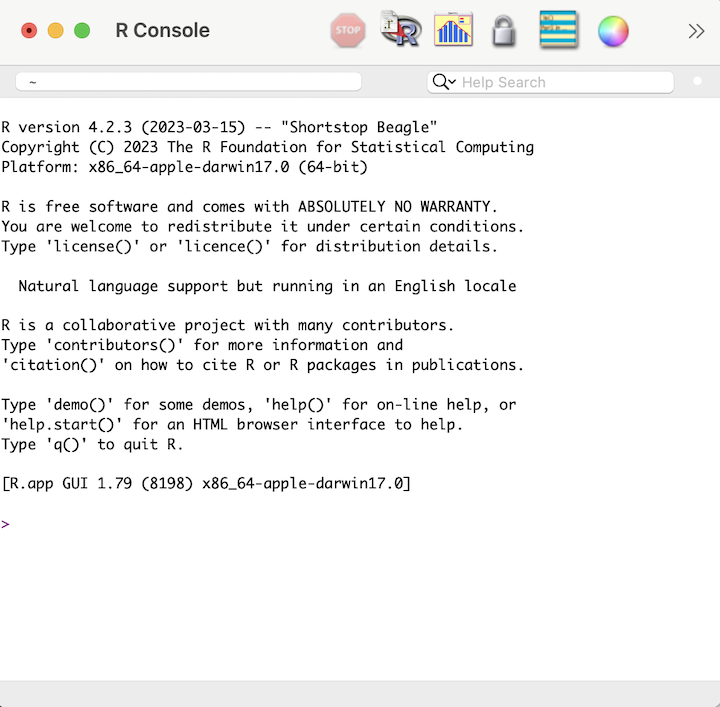
\includegraphics[width=0.4\textwidth,height=\textheight]{book/images/1-r-console.png}

}

\caption{\label{fig-r-console}The R Console.}

\end{figure}

To start, type \texttt{2+3} and press ENTER. You should see that
\texttt{5} is printed below that code and that your cursor is moved to
the next line.

\hypertarget{basic-computations-and-objects}{%
\subsection{Basic Computations and
Objects}\label{basic-computations-and-objects}}

In the example above, we coded a simple addition. Try out some other
basic calculations using the following operators:

\begin{itemize}
\tightlist
\item
  Addition: \texttt{5+6}\\
\item
  Subtraction: \texttt{7-2}\\
\item
  Multiplication: \texttt{2*3}\\
\item
  Division: \texttt{6/3}\\
\item
  Exponentiation: \texttt{4\^{}2}\\
\item
  Modulo: \texttt{100\ \%\%\ 4}
\end{itemize}

For example, use the modulo operator to find what 100 mod 4 is. It
should return 0 since 100 is divisible by 4.

If we want to save the result of any computation, we need to create an
object to store our value of interest. An \textbf{object} is simply a
named data structure that allows us to reference that data structure.
Objects are also commonly called \textbf{variables}. In the code below,
we create an object \texttt{x} which stores the value \texttt{5} using
the assignment operator \texttt{\textless{}-}. The assignment operator
assigns whatever is on the right hand side of the operator to the name
on the left hand side. We can now reference \texttt{x} by calling its
name. Additionally, we can update its value by adding 1. In the second
line of code, the computer first finds the value of the right hand side
by finding the current value of \texttt{x} before adding 1 and assigning
it back to \texttt{x}.

\begin{Shaded}
\begin{Highlighting}[]
\NormalTok{x }\OtherTok{\textless{}{-}} \DecValTok{2}\SpecialCharTok{+}\DecValTok{3}
\NormalTok{x }\OtherTok{\textless{}{-}}\NormalTok{ x}\SpecialCharTok{+}\DecValTok{1}
\NormalTok{x}
\CommentTok{\#\textgreater{} [1] 6}
\end{Highlighting}
\end{Shaded}

We can create and store multiple objects by using different names. The
code below creates a new object \texttt{y} that is one more than the
value of \texttt{x}. We can see that the value of \texttt{x} is still
\texttt{5} after running this code.

\begin{Shaded}
\begin{Highlighting}[]
\NormalTok{x }\OtherTok{\textless{}{-}} \DecValTok{2}\SpecialCharTok{+}\DecValTok{3}
\NormalTok{y }\OtherTok{\textless{}{-}}\NormalTok{ x}
\NormalTok{y }\OtherTok{\textless{}{-}}\NormalTok{ y }\SpecialCharTok{+} \DecValTok{1}
\NormalTok{x}
\CommentTok{\#\textgreater{} [1] 5}
\end{Highlighting}
\end{Shaded}

\hypertarget{naming-conventions}{%
\subsection{Naming Conventions}\label{naming-conventions}}

As we start creating objects, we want to make sure we use good object
names. Here are a few tips for naming objects effectively:

\begin{itemize}
\tightlist
\item
  Stick to a single format. We will use \textbf{snake\_case}, which uses
  underscores between words (e.g.~\texttt{my\_var},
  \texttt{class\_year}).\\
\item
  Make your names useful. Try to avoid using names that are too long\\
  (e.g.~\texttt{which\_day\_of\_the\_week}) or do not contain enough
  information (e.g., \texttt{x1}, \texttt{x2}, \texttt{x3}).\\
\item
  Replace unexplained values with an object. For example, if you need to
  do some calculations using 100 as the number of participants, create
  an object \texttt{n\_part} with value 100 rather than repeatedly using
  the number. This makes the code easy to update and helps the user
  avoid possible errors.
\end{itemize}

\hypertarget{rstudio-and-r-markdown}{%
\section{RStudio and R Markdown}\label{rstudio-and-r-markdown}}

If we made a mistake in the code above, we would have to retype
everything from the beginning. However, when we write code, we often
want to be able to run it multiple times and develop it in stages. R
scripts and R markdown files allow us to save all of our R code in files
that we can update and re-run, which allows us to create reproducible
and shareable analyses. We will now move to RStudio as our development
environment to demonstrate creating an R script. When you open RStudio,
you will see multiple windows. Start by opening a new R file by going to
File -\textgreater{} New File -\textgreater{} R Script. You should now
see several windows as shown in Figure~\ref{fig-rstudio}.

\begin{figure}

{\centering 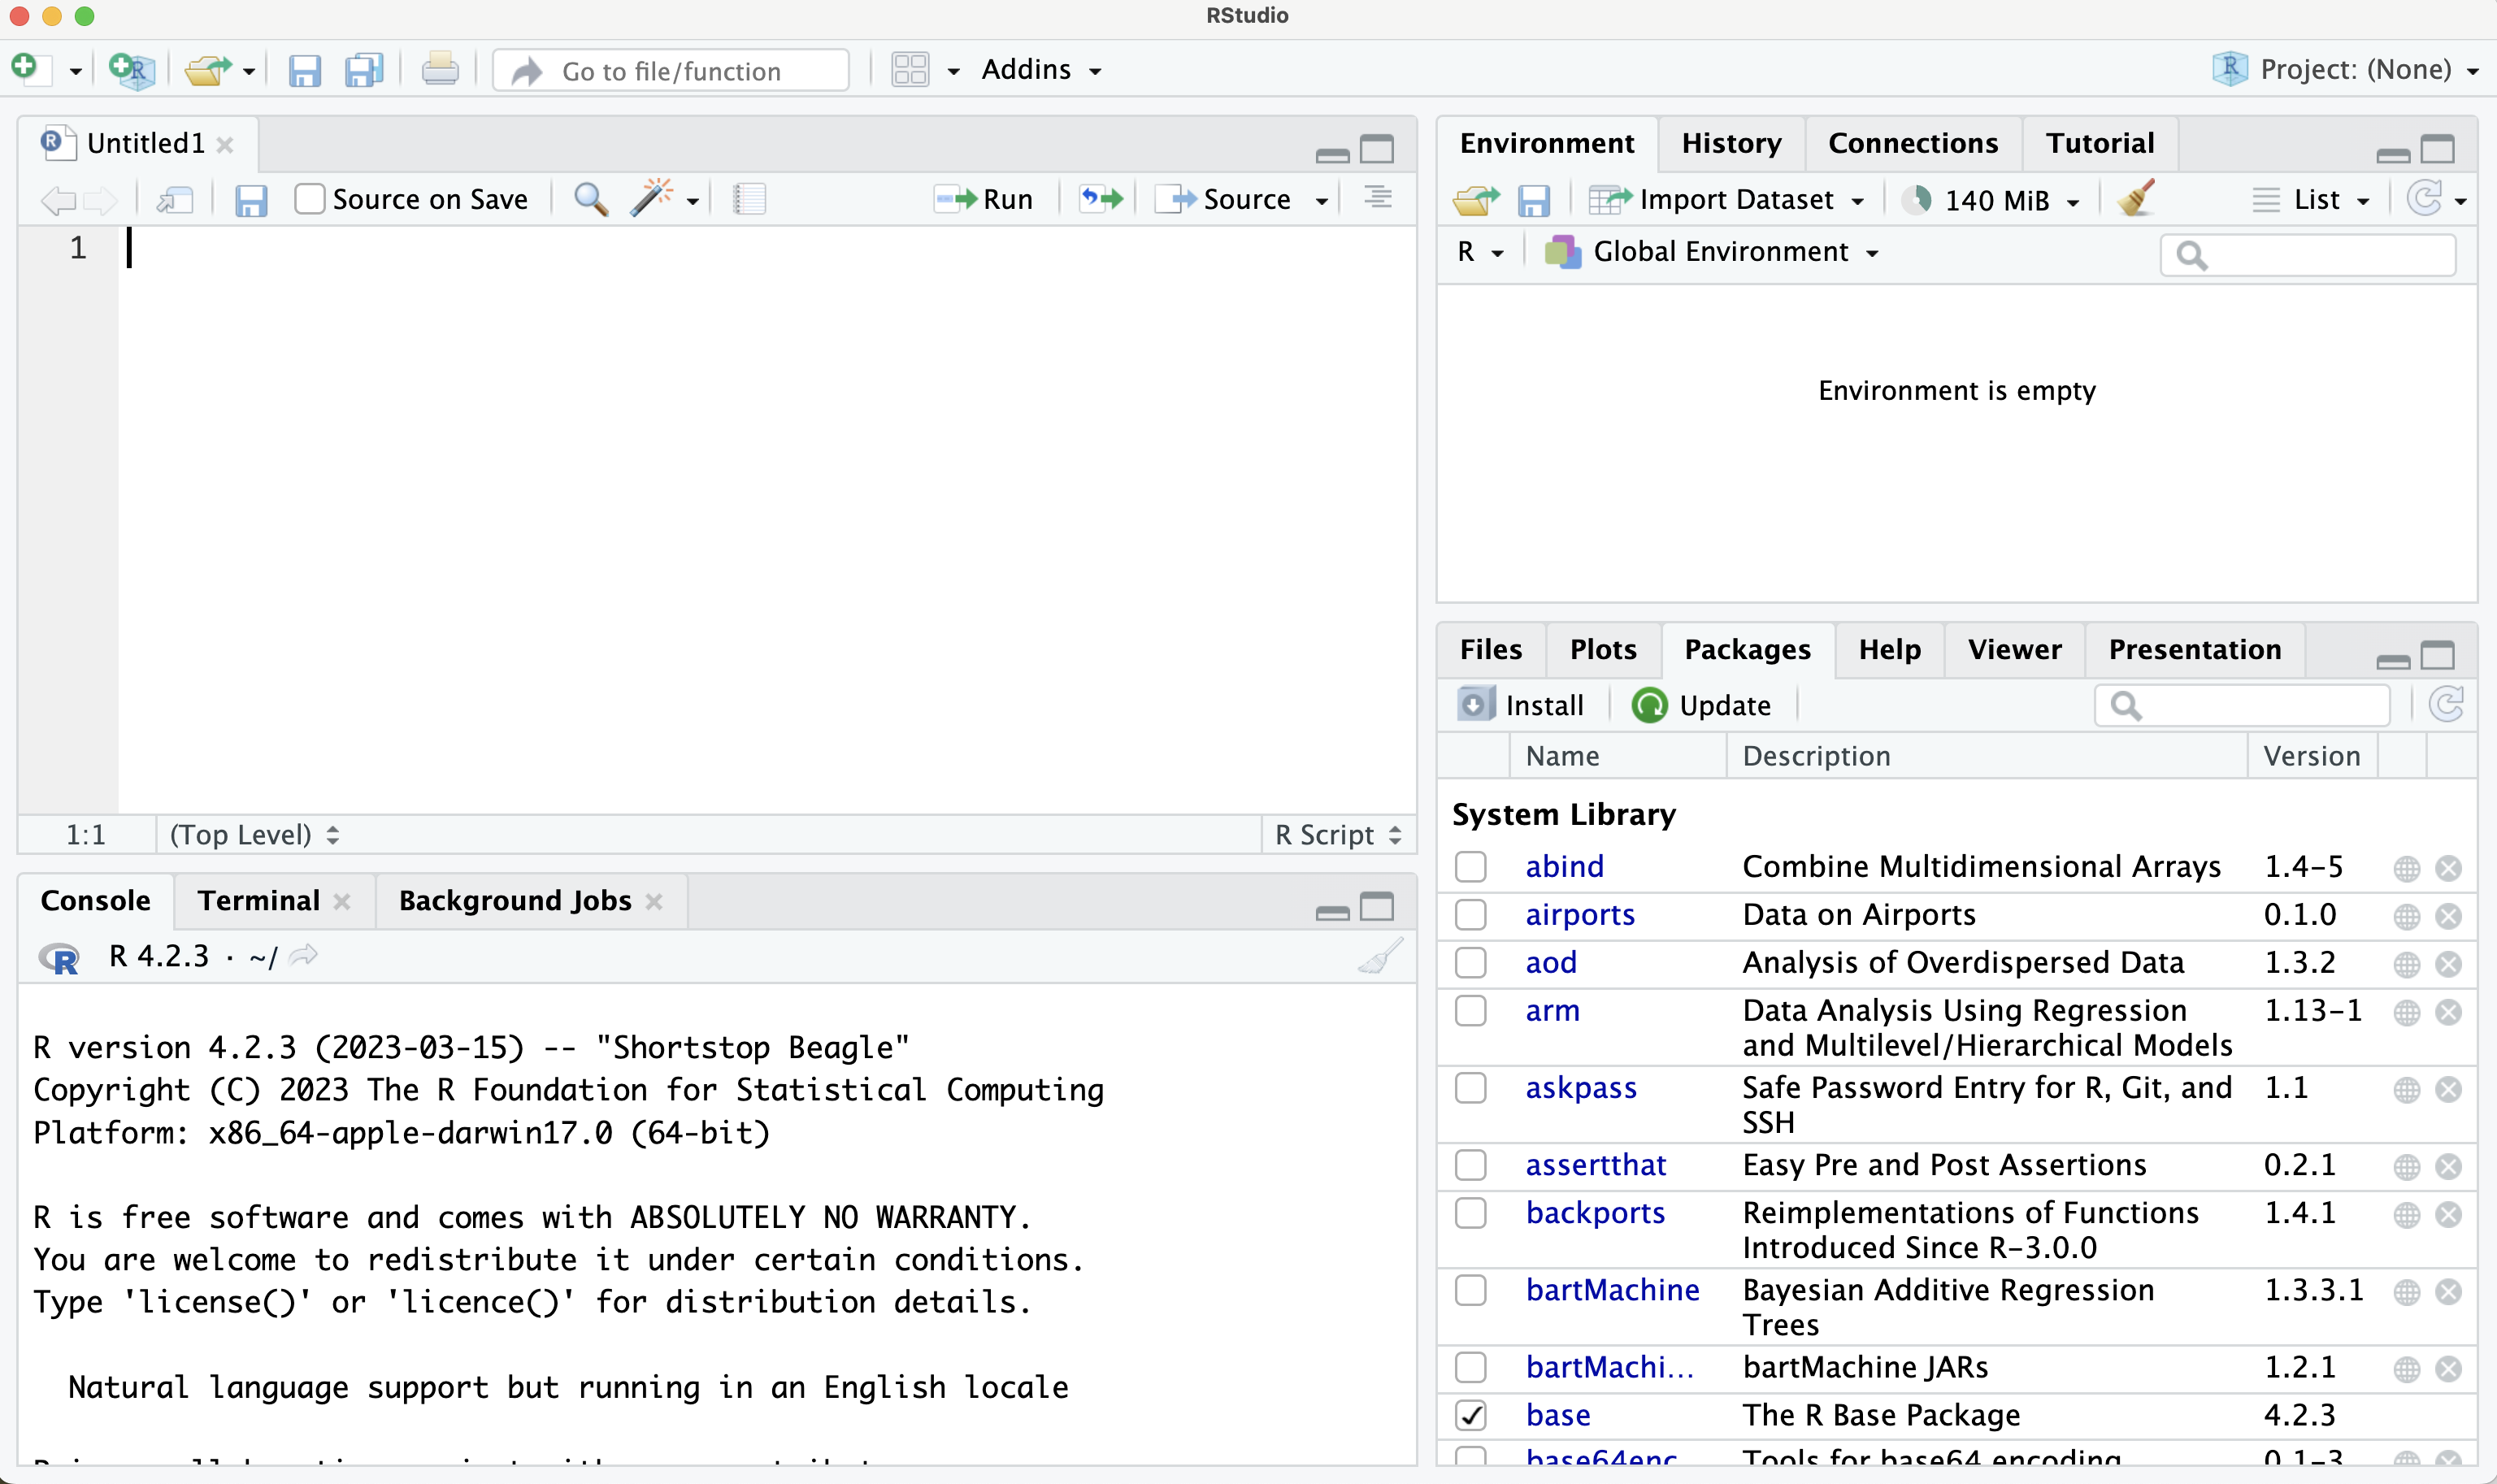
\includegraphics[width=4.16667in,height=\textheight]{book/images/1-rstudio.png}

}

\caption{\label{fig-rstudio}RStudio Layout and Panes.}

\end{figure}

In the code editor window in the top left, add the following code to
your .R file and save the file. Note that here we used snake\_case to
name our objects!

\begin{Shaded}
\begin{Highlighting}[]
\CommentTok{\# Calculate student to faculty ratio, 2023 enrollment}
\NormalTok{num\_students }\OtherTok{\textless{}{-}} \DecValTok{132}
\NormalTok{num\_faculty }\OtherTok{\textless{}{-}} \DecValTok{23}
\NormalTok{student\_fac\_ratio }\OtherTok{\textless{}{-}}\NormalTok{ num\_students}\SpecialCharTok{/}\NormalTok{num\_faculty}
\end{Highlighting}
\end{Shaded}

The first line starts with \texttt{\#} and does not contain any code.
This is a comment line, which allows us to add context, intent, or extra
information to help the reader understand our code. A good rule of thumb
is that we want to write enough comments so that we could open our code
in six months and be able to understand what we were doing. As we
develop longer chunks of code, this will become more important.

\hypertarget{calling-functions}{%
\subsection{Calling Functions}\label{calling-functions}}

When we use R, we have access to all the functions available in base R.
A \textbf{function} takes in one or more inputs and returns a single
output object. Let's first use the simple function \texttt{exp()}. This
exponential function takes in one (or more) numeric values and
exponentiates them. The code below computes \(e^3\).

\begin{Shaded}
\begin{Highlighting}[]
\FunctionTok{exp}\NormalTok{(}\DecValTok{3}\NormalTok{)}
\CommentTok{\#\textgreater{} [1] 20.1}
\end{Highlighting}
\end{Shaded}

Some other simple functions are shown below that all convert a numeric
input to an integer value. The \texttt{ceiling()} and \texttt{floor()}
functions returns the ceiling and floor of your input, and the
\texttt{round()} function will round your input to the closest integer.
Note that the \texttt{round()} function will round a 5 to the closest
even integer.

\begin{Shaded}
\begin{Highlighting}[]
\FunctionTok{ceiling}\NormalTok{(}\FloatTok{3.7}\NormalTok{)}
\CommentTok{\#\textgreater{} [1] 4}
\end{Highlighting}
\end{Shaded}

\begin{Shaded}
\begin{Highlighting}[]
\FunctionTok{floor}\NormalTok{(}\FloatTok{3.7}\NormalTok{)}
\CommentTok{\#\textgreater{} [1] 3}
\end{Highlighting}
\end{Shaded}

\begin{Shaded}
\begin{Highlighting}[]
\FunctionTok{round}\NormalTok{(}\FloatTok{2.5}\NormalTok{)}
\CommentTok{\#\textgreater{} [1] 2}
\FunctionTok{round}\NormalTok{(}\FloatTok{3.5}\NormalTok{)}
\CommentTok{\#\textgreater{} [1] 4}
\end{Highlighting}
\end{Shaded}

If we want to learn about a function, we can use the help operator
\texttt{?} by typing it in front of the function you are interested in:
this will bring up the documentation for that particular function. This
documentation will often tell you the usage of the function, the
\textbf{arguments} (the object inputs), the \textbf{value} (information
about the returned object), and will give some examples of how to use
the function. For example, if we want to understand the difference
between \texttt{floor()} and \texttt{ceiling()}, we can call
\texttt{?floor} and \texttt{?ceiling}. This should bring up the
documentation in your help window. We can then read that the floor
function rounds a numeric input down to the nearest integer whereas the
ceiling function rounds a numeric input up to the nearest integer.

\hypertarget{working-directories-and-paths}{%
\subsection{Working Directories and
Paths}\label{working-directories-and-paths}}

Let's try using another example function: \texttt{read.csv()}. This
function reads in a comma-delimited file and returns the information as
a data frame (try typing \texttt{?read.csv} in the console to read more
about this function). We will learn more about data frames in
Chapter~\ref{sec-data-structures}. The first argument to this function
is a file, which can be expressed as either a filename or a path to a
file. First, download the file \texttt{fake\_names.csv} from this book's
\href{https://github.com/alicepaul/health-data-science-using-r/tree/main/book/data}{github
repository}. By default, R will look for the file in your current
working directory. To find the working directory, you can run
\texttt{getwd()}. You can see below that my current working directory is
where the book content is on my computer.

\begin{Shaded}
\begin{Highlighting}[]
\FunctionTok{getwd}\NormalTok{()}
\CommentTok{\#\textgreater{} [1] "/Users/alice/Dropbox/health{-}data{-}science{-}using{-}r/book"}
\end{Highlighting}
\end{Shaded}

You can either move the .csv file to your current working directory and
load it in, or you can specify the path to the .csv file. Another option
is to update your working directory by using the \texttt{setwd()}
function.

\begin{Shaded}
\begin{Highlighting}[]
\FunctionTok{setwd}\NormalTok{(}\StringTok{\textquotesingle{}/Users/Alice/Dropbox/health{-}data{-}science{-}using{-}r/book/data\textquotesingle{}}\NormalTok{)}
\end{Highlighting}
\end{Shaded}

If you receive an error that a file cannot be found, you most likely
have the wrong path to the file or the wrong file name. Below, I chose
to specify the path to the downloaded .csv file, saved this file to an
object called \texttt{df}, and then printed that \texttt{df} object.

\begin{Shaded}
\begin{Highlighting}[]
\NormalTok{df }\OtherTok{\textless{}{-}} \FunctionTok{read.csv}\NormalTok{(}\StringTok{"data/fake\_names.csv"}\NormalTok{) }\CommentTok{\# update this with the path to your file}
\NormalTok{df}
\CommentTok{\#\textgreater{}                  Name Age     DOB            City State}
\CommentTok{\#\textgreater{} 1           Ken Irwin  37 6/28/85      Providence    RI}
\CommentTok{\#\textgreater{} 2 Delores Whittington  56 4/28/67      Smithfield    RI}
\CommentTok{\#\textgreater{} 3       Daniel Hughes  41 5/22/82      Providence    RI}
\CommentTok{\#\textgreater{} 4         Carlos Fain  83  2/2/40          Warren    RI}
\CommentTok{\#\textgreater{} 5        James Alford  67 2/23/56 East Providence    RI}
\CommentTok{\#\textgreater{} 6        Ruth Alvarez  34 9/22/88      Providence    RI}
\end{Highlighting}
\end{Shaded}

We can see that \texttt{df} contains the information from the .csv file
and that R has printed the first few observations of the data.

\hypertarget{installing-and-loading-packages}{%
\subsection{Installing and Loading
Packages}\label{installing-and-loading-packages}}

When working with data frames, we will often use the \textbf{tidyverse}
package (Wickham 2023), which is actually a collection of R packages for
data science applications. An R package is a collection of functions
and/or sample data that allow us to expand on the functionality of R
beyond the base functions. You can check whether you have the
\textbf{tidyverse} package installed by going to the package pane in
RStudio or by running the command below, which will display all your
installed packages.

\texttt{installed.packages()}

If you don't already have a package installed, you can install it using
the \texttt{install.packages()} function. Note that you have to include
single or double quotes around the package name when using this
function. You only have to install a package one time.

\texttt{install.packages(\textquotesingle{}tidyverse\textquotesingle{})}

The function \texttt{read\_csv()} is another function to read in
comma-delimited files that is part of the \textbf{readr} package in the
tidyverse. However, if we tried to use this function to load in our
data, we would get an error that the function cannot be found. That is
because we haven't loaded in this package. To do so, we use the
\texttt{library()} function. Unlike the \texttt{install.packages()}
function, we do not have to use quotes around the package name when
calling this \texttt{library()} function. When we load in a package, we
will see some messages. For example, below we see that this package
contains the functions \texttt{filter()} and \texttt{lag()} that are
also functions in base R. In future chapters, we will suppress these
messages to make the chapter presentation nicer. After loading the
\textbf{tidyverse} package, we can now use the \texttt{read\_csv()}
function as shown below.

\begin{Shaded}
\begin{Highlighting}[]
\FunctionTok{library}\NormalTok{(tidyverse)}
\end{Highlighting}
\end{Shaded}

\begin{Shaded}
\begin{Highlighting}[]
\NormalTok{df }\OtherTok{\textless{}{-}} \FunctionTok{read\_csv}\NormalTok{(}\StringTok{"data/fake\_names.csv"}\NormalTok{, }\AttributeTok{show\_col\_types=}\ConstantTok{FALSE}\NormalTok{)}
\NormalTok{df}
\CommentTok{\#\textgreater{} \# A tibble: 6 x 5}
\CommentTok{\#\textgreater{}   Name                  Age DOB     City            State}
\CommentTok{\#\textgreater{}   \textless{}chr\textgreater{}               \textless{}dbl\textgreater{} \textless{}chr\textgreater{}   \textless{}chr\textgreater{}           \textless{}chr\textgreater{}}
\CommentTok{\#\textgreater{} 1 Ken Irwin              37 6/28/85 Providence      RI   }
\CommentTok{\#\textgreater{} 2 Delores Whittington    56 4/28/67 Smithfield      RI   }
\CommentTok{\#\textgreater{} 3 Daniel Hughes          41 5/22/82 Providence      RI   }
\CommentTok{\#\textgreater{} 4 Carlos Fain            83 2/2/40  Warren          RI   }
\CommentTok{\#\textgreater{} 5 James Alford           67 2/23/56 East Providence RI   }
\CommentTok{\#\textgreater{} \# i 1 more row}
\end{Highlighting}
\end{Shaded}

Alternatively, we could have told R where to locate the function by
adding \texttt{readr::} before the function. This tells it to find
\texttt{read\_csv()} function in the \textbf{readr} package. This can be
helpful even if we have already loaded in the package, since sometimes
multiple packages have functions with the same name.

\begin{Shaded}
\begin{Highlighting}[]
\NormalTok{df }\OtherTok{\textless{}{-}}\NormalTok{ readr}\SpecialCharTok{::}\FunctionTok{read\_csv}\NormalTok{(}\StringTok{"data/fake\_names.csv"}\NormalTok{, }\AttributeTok{show\_col\_types =} \ConstantTok{FALSE}\NormalTok{)}
\end{Highlighting}
\end{Shaded}

\hypertarget{rstudio-global-options}{%
\subsection{RStudio Global Options}\label{rstudio-global-options}}

You have now had a basic tour of RStudio. We highly recommend that you
update your RStudio options to not save your workspace on exiting or
load it on starting. This will ensure that you create fully reproducible
code and avoid possible errors or confusion.

\begin{figure}

{\centering 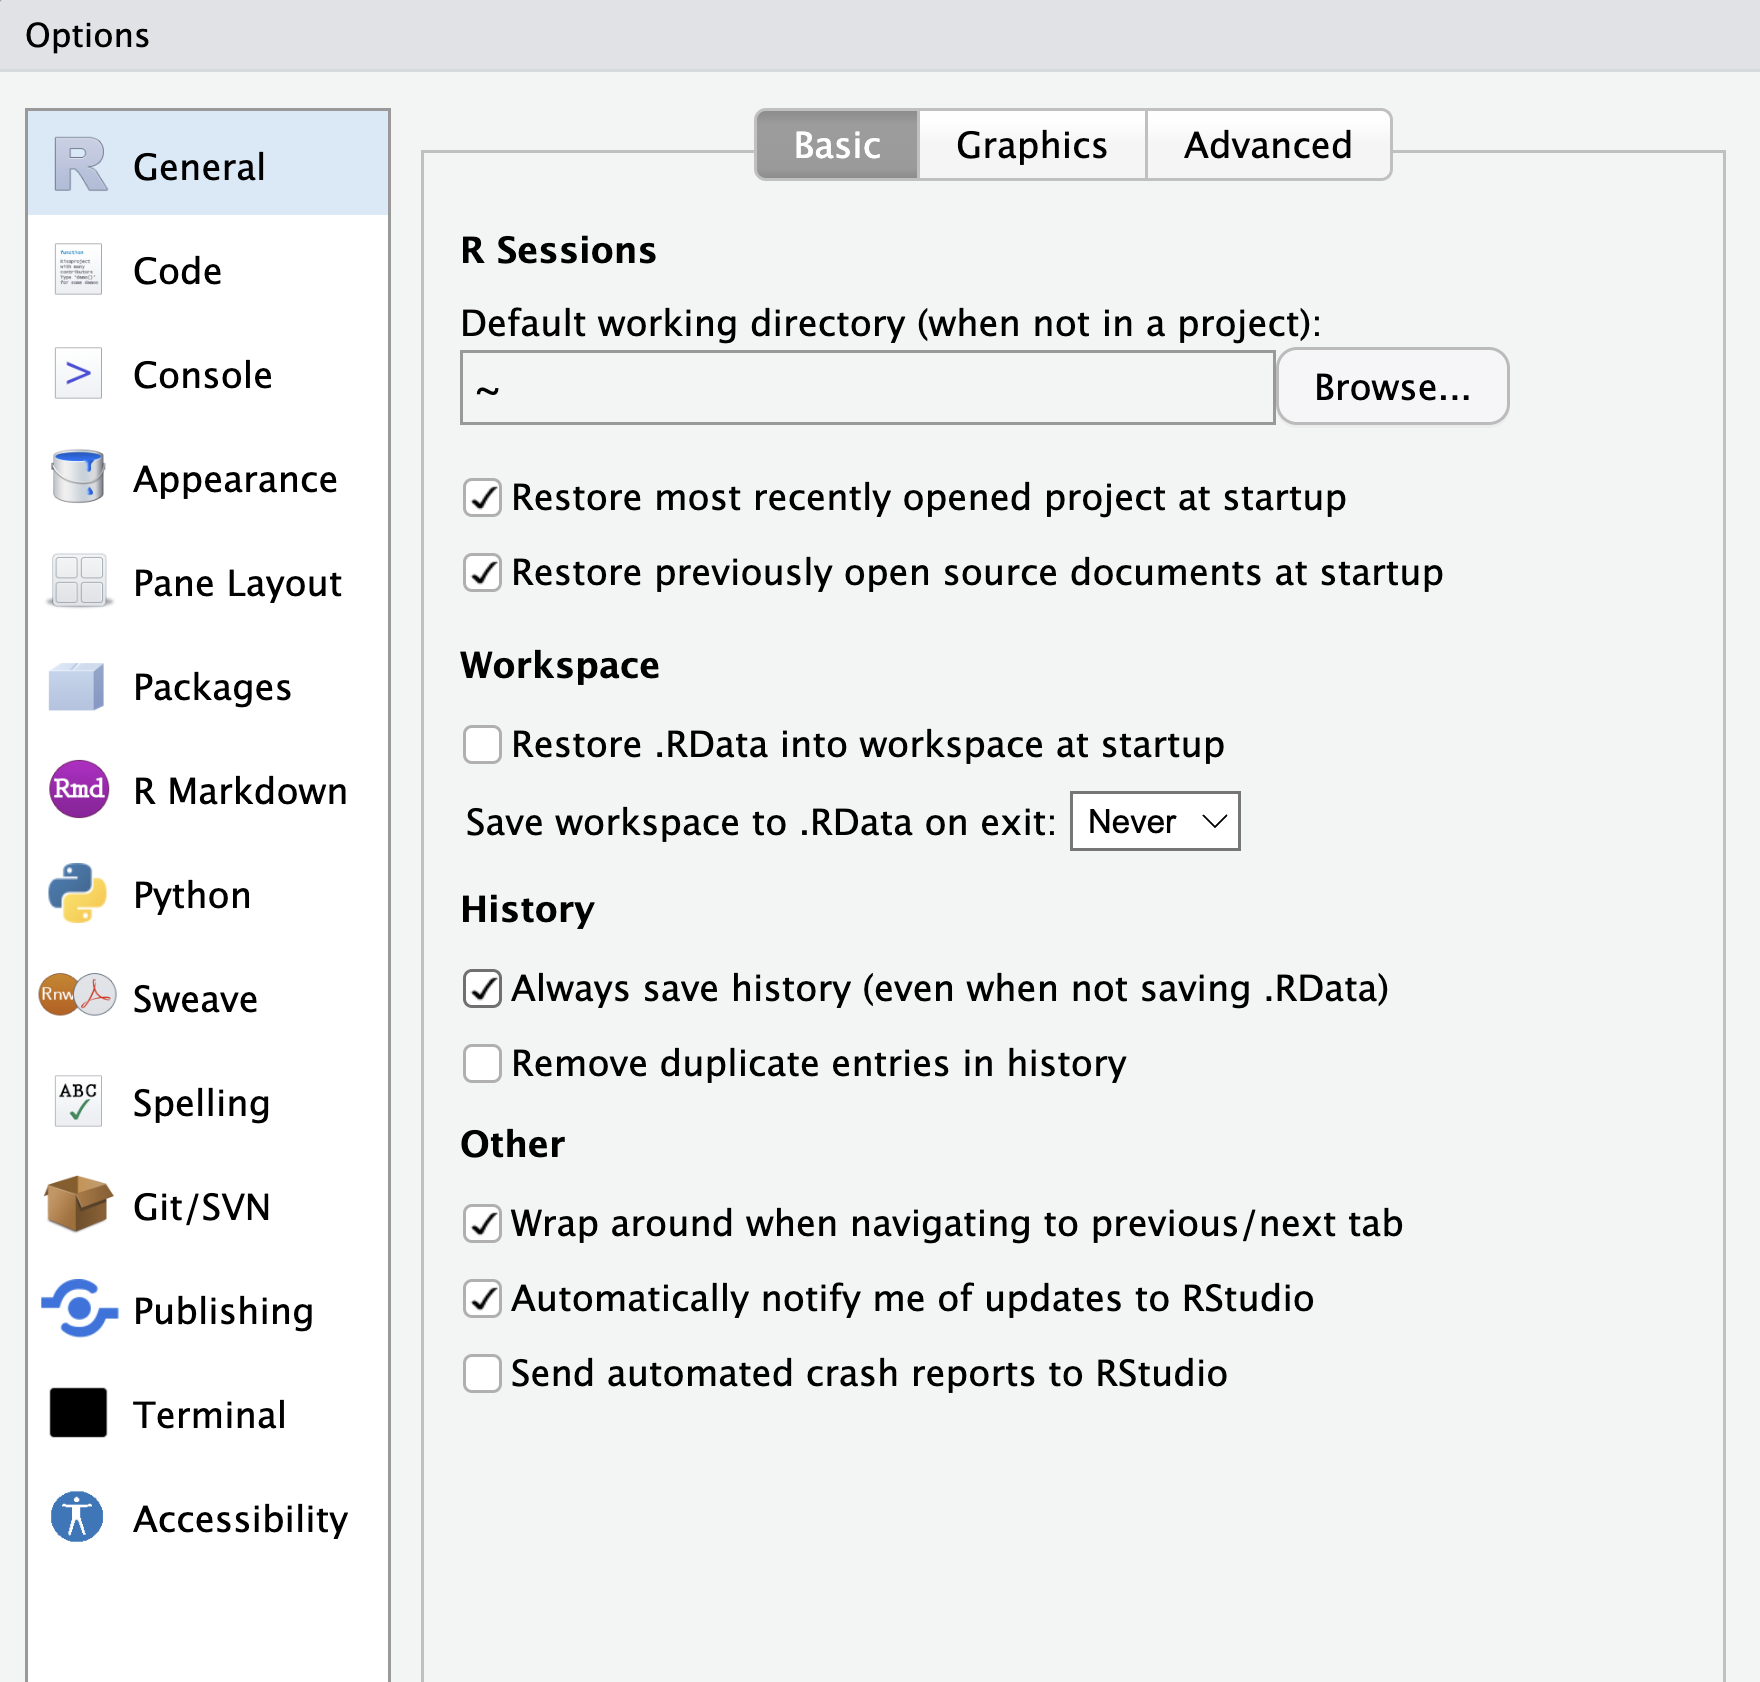
\includegraphics[width=0.4\textwidth,height=\textheight]{book/images/1-rstudio-global-opts.png}

}

\caption{\label{fig-global-options}RStudio Global Options.}

\end{figure}

\hypertarget{tips-and-reminders}{%
\section{Tips and Reminders}\label{tips-and-reminders}}

We end this chapter with some final tips and reminders.

\begin{itemize}
\item
  \textbf{Keyboard Shortcuts}: RStudio has several useful keyboard
  shortcuts that will make your programming experience more streamlined.
  It is worth getting familiar with some of the most common keyboard
  shortcuts using this book's
  \href{https://github.com/alicepaul/health-data-science-using-r/blob/main/book/refs/}{cheatsheet}.
\item
  \textbf{Asking for help}: Within R, you can use the \texttt{?}
  operator or the \texttt{help()} function to pull up documentation on a
  given function. This documentation is also available
  \href{https://rdocumentation.org/}{online}.
\item
  \textbf{Finding all objects}: You can use the Environment panel or
  \texttt{ls()} function to find all current objects. If you have an
  error that an object you are calling does not exist, take a look to
  find where you defined it.
\item
  \textbf{Checking packages}: If you get an error that a function does
  not exist, check to make sure you have loaded that package using the
  \texttt{library()} function. The list of packages used in this book is
  given on the github repository homepage.
\end{itemize}

\bookmarksetup{startatroot}

\hypertarget{sec-data-structures}{%
\chapter{Data Structures in R}\label{sec-data-structures}}

In this chapter, we will demonstrate the key \textbf{data structures} in
R. Data structures are how information is stored in R, and the data
structures that we use inform R how to interpret our code. Any
\textbf{object} is a named instance of a data structure. For example,
the object \texttt{ex\_num} below is a vector of numeric type.

\begin{Shaded}
\begin{Highlighting}[]
\NormalTok{ex\_num }\OtherTok{\textless{}{-}} \DecValTok{4}
\end{Highlighting}
\end{Shaded}

The main data structures in R are \textbf{vectors}, \textbf{factors},
\textbf{matrices}, \textbf{arrays}, \textbf{lists}, and \textbf{data
frames}. These structures are distinguished by their dimensions and by
the type of data they store. For example, we might have a 1-dimensional
vector that contains all numeric values, or we could have a
2-dimensional data frame with rows and columns where we might have one
numeric column and one character column. In the image below, there are
two vectors with different types (character and numeric) on top and then
a matrix and data frame below. In this chapter, we will cover each data
structure except for arrays. Arrays are an extension of matrices that
allow for data that is more than 2-dimensional and are not needed for
the applications covered in this book.

\hypertarget{data-types}{%
\section{Data Types}\label{data-types}}

Each individual value in R has a type: \textbf{logical},
\textbf{integer}, \textbf{double}, or \textbf{character}. We can think
of these as the building blocks of all data structures. Below, we can
use the \texttt{typeof()} function to find the type of our vector from
above, which shows that the value of \texttt{ex\_num} is a
\textbf{double}. A double is a numeric value with a stored decimal.

\begin{Shaded}
\begin{Highlighting}[]
\FunctionTok{typeof}\NormalTok{(ex\_num)}
\CommentTok{\#\textgreater{} [1] "double"}
\end{Highlighting}
\end{Shaded}

On the other hand, an \textbf{integer} is a whole number that does not
contain a decimal. We now create an integer object \texttt{ex\_int}. To
indicate to R that we want to restrict our values to integer values, we
use an \texttt{L} after the number.

\begin{Shaded}
\begin{Highlighting}[]
\NormalTok{ex\_int }\OtherTok{\textless{}{-}}\NormalTok{ 4L}
\FunctionTok{typeof}\NormalTok{(ex\_int)}
\CommentTok{\#\textgreater{} [1] "integer"}
\end{Highlighting}
\end{Shaded}

Both \texttt{ex\_num} and \texttt{ex\_int} are numeric objects, but we
can also work with two other types of objects: \textbf{characters}
(e.g.~``php'', ``stats'') and \textbf{booleans} (e.g.~TRUE, FALSE), also
known as \textbf{logicals}.

\begin{Shaded}
\begin{Highlighting}[]
\NormalTok{ex\_bool }\OtherTok{\textless{}{-}} \ConstantTok{TRUE}
\NormalTok{ex\_char }\OtherTok{\textless{}{-}} \StringTok{"Alice"}

\FunctionTok{typeof}\NormalTok{(ex\_bool)}
\CommentTok{\#\textgreater{} [1] "logical"}
\FunctionTok{typeof}\NormalTok{(ex\_char)}
\CommentTok{\#\textgreater{} [1] "character"}
\end{Highlighting}
\end{Shaded}

One important characteristic of logical objects is that R will also
interpret them as 0/1. This means they can be added as in the example
below: each \texttt{TRUE} has a value of 1 and each \texttt{FALSE} has a
value of 0.

\begin{Shaded}
\begin{Highlighting}[]
\ConstantTok{TRUE}\SpecialCharTok{+}\ConstantTok{FALSE}\SpecialCharTok{+}\ConstantTok{TRUE}
\CommentTok{\#\textgreater{} [1] 2}
\end{Highlighting}
\end{Shaded}

To create all of the above objects, we used the assignment operator
\texttt{\textless{}-}, which we discussed in
Chapter~\ref{sec-intro-to-r}. You may see code elsewhere that uses an
\texttt{=} instead. While \texttt{=} can also be used for assignment, it
is more standard practice to use \texttt{\textless{}-}.

\hypertarget{vectors}{%
\section{Vectors}\label{vectors}}

In the examples above, we created objects with a single value. R
actually uses a vector of length 1 to store this information.
\textbf{Vectors} are 1-dimensional data structures that can store
multiple data values of the same type (e.g.~character, boolean, or
numeric).

\begin{figure}

{\centering 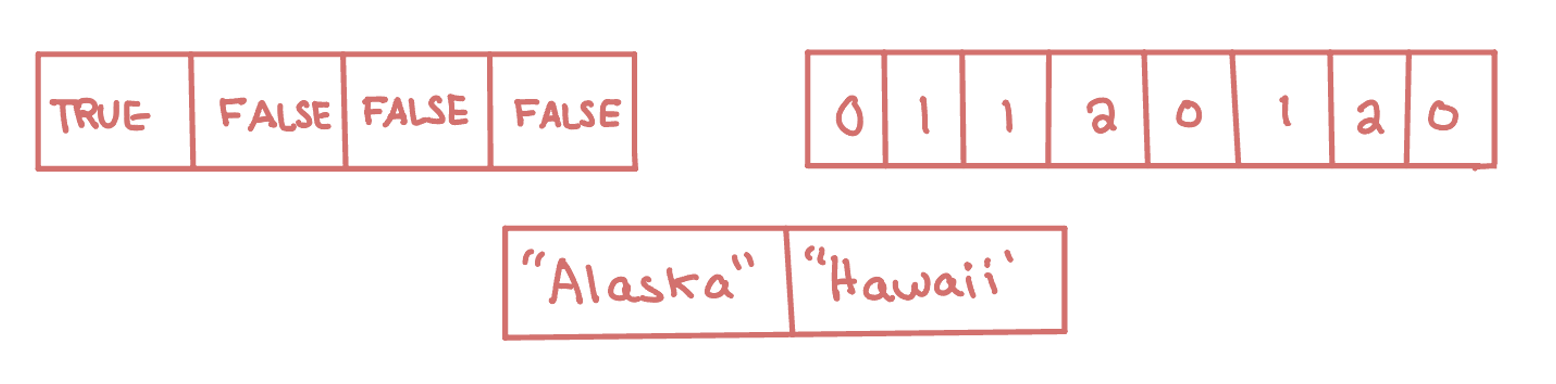
\includegraphics{book/images/2-vectors.png}

}

\caption{\label{fig-vectors}Vector Examples.}

\end{figure}

We can confirm this by using the \texttt{is.vector()} function, which
returns whether or not the inputted argument is a vector.

\begin{Shaded}
\begin{Highlighting}[]
\FunctionTok{is.vector}\NormalTok{(ex\_bool)}
\CommentTok{\#\textgreater{} [1] TRUE}
\end{Highlighting}
\end{Shaded}

One way to create a vector with multiple values is to use the combine
function \texttt{c()}. Below we create two vectors: one with the days of
the week and one with the amount of rain on each day. The first vector
has all character values, and the second one has all numeric values.

\begin{Shaded}
\begin{Highlighting}[]
\NormalTok{days }\OtherTok{\textless{}{-}} \FunctionTok{c}\NormalTok{(}\StringTok{"Monday"}\NormalTok{, }\StringTok{"Tuesday"}\NormalTok{, }\StringTok{"Wednesday"}\NormalTok{, }\StringTok{"Thursday"}\NormalTok{, }\StringTok{"Friday"}\NormalTok{)}
\NormalTok{rain }\OtherTok{\textless{}{-}} \FunctionTok{c}\NormalTok{(}\DecValTok{5}\NormalTok{, }\FloatTok{0.1}\NormalTok{, }\DecValTok{0}\NormalTok{, }\DecValTok{0}\NormalTok{, }\FloatTok{0.4}\NormalTok{)}
\end{Highlighting}
\end{Shaded}

Remember, vectors cannot store objects of different types. Because of
this, in the code below, R automatically converts the numeric value to
be a character in order to store these values in a vector together.

\begin{Shaded}
\begin{Highlighting}[]
\FunctionTok{c}\NormalTok{(}\StringTok{"Monday"}\NormalTok{, }\DecValTok{5}\NormalTok{)}
\CommentTok{\#\textgreater{} [1] "Monday" "5"}
\end{Highlighting}
\end{Shaded}

The \texttt{class()} function returns the data structure of an object.
If we check the classes of these two objects using the \texttt{class()}
function, we will see that R tells us that the first is a character
vector and the second is a numeric vector. This matches the data type in
this case.

\begin{Shaded}
\begin{Highlighting}[]
\FunctionTok{class}\NormalTok{(days)}
\CommentTok{\#\textgreater{} [1] "character"}
\FunctionTok{class}\NormalTok{(rain)}
\CommentTok{\#\textgreater{} [1] "numeric"}
\end{Highlighting}
\end{Shaded}

What happens when we create an empty vector? What is the class?

\begin{Shaded}
\begin{Highlighting}[]
\NormalTok{ex\_empty }\OtherTok{\textless{}{-}} \FunctionTok{c}\NormalTok{()}
\FunctionTok{class}\NormalTok{(ex\_empty)}
\CommentTok{\#\textgreater{} [1] "NULL"}
\end{Highlighting}
\end{Shaded}

In this case, there is no specified type yet. If we wanted to specify
the type, we could make an empty vector using the \texttt{vector()}
function.

\begin{Shaded}
\begin{Highlighting}[]
\NormalTok{ex\_empty }\OtherTok{\textless{}{-}} \FunctionTok{vector}\NormalTok{(}\AttributeTok{mode =} \StringTok{"numeric"}\NormalTok{)}
\FunctionTok{class}\NormalTok{(ex\_empty)}
\CommentTok{\#\textgreater{} [1] "numeric"}
\end{Highlighting}
\end{Shaded}

Another way to create a vector is with the \texttt{rep()} or
\texttt{seq()} functions. The first function \texttt{rep(x,\ times)}
takes in a vector \texttt{x} and a number of times \texttt{times} and
outputs \texttt{x} repeated that many times. Let's try this with a
single value below. The second function \texttt{seq(from,\ to,\ step)}
takes in a numeric starting value \texttt{from}, end value \texttt{to},
and step size \texttt{step} and returns a sequence from \texttt{from} in
increments of \texttt{step} until a maximum value of \texttt{to} is
reached.

\begin{Shaded}
\begin{Highlighting}[]
\FunctionTok{rep}\NormalTok{(}\DecValTok{0}\NormalTok{, }\DecValTok{5}\NormalTok{)}
\CommentTok{\#\textgreater{} [1] 0 0 0 0 0}
\FunctionTok{rep}\NormalTok{(}\StringTok{"Monday"}\NormalTok{, }\DecValTok{4}\NormalTok{)}
\CommentTok{\#\textgreater{} [1] "Monday" "Monday" "Monday" "Monday"}
\FunctionTok{seq}\NormalTok{(}\DecValTok{1}\NormalTok{, }\DecValTok{5}\NormalTok{, }\DecValTok{1}\NormalTok{)}
\CommentTok{\#\textgreater{} [1] 1 2 3 4 5}
\FunctionTok{seq}\NormalTok{(}\DecValTok{0}\NormalTok{, }\SpecialCharTok{{-}}\DecValTok{10}\NormalTok{, }\SpecialCharTok{{-}}\DecValTok{2}\NormalTok{)}
\CommentTok{\#\textgreater{} [1]   0  {-}2  {-}4  {-}6  {-}8 {-}10}
\end{Highlighting}
\end{Shaded}

\hypertarget{indexing-a-vector}{%
\subsection{Indexing a Vector}\label{indexing-a-vector}}

Once we have a vector, we may want to access certain values stored in
that vector. To do so, we index the vector using the position of each
value: the first value in the vector has index 1, the second value has
index 2, etc. When we say a vector is 1-dimensional, we mean that we can
define the position of each value by a single index. To index the
vector, we then use square brackets \texttt{{[}{]}} after the vector
name and provide the position. Below, we use these indices to find the
value at index 1 and the value at index 4.

\begin{Shaded}
\begin{Highlighting}[]
\NormalTok{days[}\DecValTok{1}\NormalTok{]}
\CommentTok{\#\textgreater{} [1] "Monday"}
\NormalTok{days[}\DecValTok{4}\NormalTok{]}
\CommentTok{\#\textgreater{} [1] "Thursday"}
\end{Highlighting}
\end{Shaded}

We can either access a single value or a subset of values using a vector
of indices. Let's see what happens when we use a vector of indices
\texttt{c(1,4)} and then try using \texttt{-c(1,4)} and see what happens
then. In the first case, we get the values at index 1 \emph{and} at
index 4. In the second case, we get all values \emph{except} at those
indices. The \texttt{-} indicates that we want to remove rather than
select these indices.

\begin{Shaded}
\begin{Highlighting}[]
\NormalTok{days[}\FunctionTok{c}\NormalTok{(}\DecValTok{1}\NormalTok{,}\DecValTok{4}\NormalTok{)]}
\CommentTok{\#\textgreater{} [1] "Monday"   "Thursday"}
\NormalTok{days[}\SpecialCharTok{{-}}\FunctionTok{c}\NormalTok{(}\DecValTok{1}\NormalTok{,}\DecValTok{4}\NormalTok{)]}
\CommentTok{\#\textgreater{} [1] "Tuesday"   "Wednesday" "Friday"}
\end{Highlighting}
\end{Shaded}

However, always indexing by the index value can sometimes be difficult
or inefficient. One extra feature of vectors is that we can associate a
name with each value. Below, we update the names of the vector
\texttt{rain} to be the days of the week and then find Friday's rain
count by indexing with the name.

\begin{Shaded}
\begin{Highlighting}[]
\FunctionTok{names}\NormalTok{(rain) }\OtherTok{\textless{}{-}}\NormalTok{ days}
\FunctionTok{print}\NormalTok{(rain)}
\CommentTok{\#\textgreater{}    Monday   Tuesday Wednesday  Thursday    Friday }
\CommentTok{\#\textgreater{}       5.0       0.1       0.0       0.0       0.4}
\NormalTok{rain[}\StringTok{"Friday"}\NormalTok{]}
\CommentTok{\#\textgreater{} Friday }
\CommentTok{\#\textgreater{}    0.4}
\end{Highlighting}
\end{Shaded}

The last way to index a vector is to use TRUE and FALSE values. If we
have a vector of booleans that is the same length as our original
vector, then this will return all the values that correspond to a TRUE
value. For example, indexing the \texttt{days} vector by the logical
vector \texttt{ind\_bools} below will return its first and fourth
values. We will see more about using logic to access certain values
later on.

\begin{Shaded}
\begin{Highlighting}[]
\NormalTok{ind\_bools }\OtherTok{\textless{}{-}} \FunctionTok{c}\NormalTok{(}\ConstantTok{TRUE}\NormalTok{, }\ConstantTok{FALSE}\NormalTok{, }\ConstantTok{FALSE}\NormalTok{, }\ConstantTok{TRUE}\NormalTok{, }\ConstantTok{FALSE}\NormalTok{)}
\NormalTok{days[ind\_bools]}
\CommentTok{\#\textgreater{} [1] "Monday"   "Thursday"}
\end{Highlighting}
\end{Shaded}

\hypertarget{editing-a-vector-and-calculations}{%
\subsection{Editing a Vector and
Calculations}\label{editing-a-vector-and-calculations}}

The mathematical operators we saw in the last chapter (\texttt{+},
\texttt{-}, \texttt{*}, \texttt{/}, \texttt{\^{}}, \texttt{\%\%}) can
all be applied to numeric vectors and will be applied element-wise. That
is, in the code below, the two vectors are added together by index. This
holds true for some of the built-in math functions as well:

\begin{itemize}
\tightlist
\item
  \texttt{exp()} - exponential
\item
  \texttt{log()} - log
\item
  \texttt{sqrt()} - square root
\item
  \texttt{abs()} - absolute value
\item
  \texttt{round()} - round to nearest integer value
\item
  \texttt{ceiling()} - round up to the nearest integer value
\item
  \texttt{floor()} - round down to the nearest integer value
\end{itemize}

\begin{Shaded}
\begin{Highlighting}[]
\FunctionTok{c}\NormalTok{(}\DecValTok{1}\NormalTok{,}\DecValTok{2}\NormalTok{,}\DecValTok{3}\NormalTok{) }\SpecialCharTok{+} \FunctionTok{c}\NormalTok{(}\DecValTok{1}\NormalTok{,}\DecValTok{1}\NormalTok{,}\DecValTok{1}\NormalTok{)}
\CommentTok{\#\textgreater{} [1] 2 3 4}
\FunctionTok{c}\NormalTok{(}\DecValTok{1}\NormalTok{,}\DecValTok{2}\NormalTok{,}\DecValTok{3}\NormalTok{) }\SpecialCharTok{+} \DecValTok{1} \CommentTok{\# equivalent to the code above}
\CommentTok{\#\textgreater{} [1] 2 3 4}
\FunctionTok{sqrt}\NormalTok{(}\FunctionTok{c}\NormalTok{(}\DecValTok{1}\NormalTok{,}\DecValTok{4}\NormalTok{,}\DecValTok{16}\NormalTok{))}
\CommentTok{\#\textgreater{} [1] 1 2 4}
\end{Highlighting}
\end{Shaded}

After we create a vector, we may need to update its values. For example,
we may want to change a specific value. We can do so using indexing.
Below, we update the rain value for Friday using the assignment
operator.

\begin{Shaded}
\begin{Highlighting}[]
\NormalTok{rain[}\StringTok{"Friday"}\NormalTok{] }\OtherTok{\textless{}{-}} \FloatTok{0.5}
\NormalTok{rain}
\CommentTok{\#\textgreater{}    Monday   Tuesday Wednesday  Thursday    Friday }
\CommentTok{\#\textgreater{}       5.0       0.1       0.0       0.0       0.5}
\end{Highlighting}
\end{Shaded}

Further, we may need to add extra entries. We can do so using the
\texttt{c()} function again but this time passing in the vector we want
to add to as our first argument. This will create a single vector with
all previous and new values. Below, we add two days to both vectors and
then check the length of the updated vector \texttt{rain}. The
\texttt{length()} function returns the length of a vector.

\begin{Shaded}
\begin{Highlighting}[]
\FunctionTok{length}\NormalTok{(rain)}
\CommentTok{\#\textgreater{} [1] 5}
\NormalTok{days }\OtherTok{\textless{}{-}} \FunctionTok{c}\NormalTok{(days,}\StringTok{"Saturday"}\NormalTok{,}\StringTok{"Sunday"}\NormalTok{) }\CommentTok{\# add the weekend with no rain}
\NormalTok{rain }\OtherTok{\textless{}{-}} \FunctionTok{c}\NormalTok{(rain,}\DecValTok{0}\NormalTok{,}\DecValTok{0}\NormalTok{)}
\FunctionTok{length}\NormalTok{(rain)}
\CommentTok{\#\textgreater{} [1] 7}
\end{Highlighting}
\end{Shaded}

We can also call some useful functions on vectors. For example, the
\texttt{sum()}, \texttt{max()}, and \texttt{min()} functions will return
the sum, maximum value, and minimum value of a vector, respectively.

\hypertarget{practice-question}{%
\subsection{Practice Question}\label{practice-question}}

Create a vector of the odd numbers from 1 to 11 using the \texttt{seq()}
function. Then, find the third value in the vector using indexing, which
should have value 5.

\begin{Shaded}
\begin{Highlighting}[]
\CommentTok{\# Insert your solution here:}
\end{Highlighting}
\end{Shaded}

\hypertarget{common-vector-functions}{%
\subsection{Common Vector Functions}\label{common-vector-functions}}

Below we list some of the most common vector functions that are
available in base R. All of these functions assume that the vector is
numeric. If we pass the function a logical vector, R will convert the
vector to 0/1 first, and if we pass the function a character vector, R
will give us an error message.

\begin{itemize}
\tightlist
\item
  \texttt{sum()} - summation
\item
  \texttt{median()} - median value
\item
  \texttt{mean()} - mean
\item
  \texttt{sd()} - standard deviation
\item
  \texttt{var()} - variance
\item
  \texttt{max()} - maximum value
\item
  \texttt{which.max()} - index of the first element with the maximum
  value
\item
  \texttt{min()} - minimum value
\item
  \texttt{which.min()} - index of the first element with the minimum
  value
\end{itemize}

Try these out using the vector \texttt{rain}. Note that R is case
sensitive - \texttt{Mean()} is considered different from
\texttt{mean()}, so if we type \texttt{Mean(rain)} R will tell us that
it cannot find this function.

\begin{Shaded}
\begin{Highlighting}[]
\FunctionTok{mean}\NormalTok{(rain)  }
\CommentTok{\#\textgreater{} [1] 0.8}
\FunctionTok{min}\NormalTok{(rain) }
\CommentTok{\#\textgreater{} [1] 0}
\FunctionTok{which.min}\NormalTok{(rain) }
\CommentTok{\#\textgreater{} Wednesday }
\CommentTok{\#\textgreater{}         3}
\end{Highlighting}
\end{Shaded}

We may also be interested in the order of the values. The
\texttt{sort()} function sorts the values of a vector, whereas the
\texttt{order()} function returns the permutation of the elements to be
in sorted order. The last line of code below sorts the days of the week
from smallest to largest rain value.

\begin{Shaded}
\begin{Highlighting}[]
\NormalTok{rain}
\CommentTok{\#\textgreater{}    Monday   Tuesday Wednesday  Thursday    Friday                     }
\CommentTok{\#\textgreater{}       5.0       0.1       0.0       0.0       0.5       0.0       0.0}
\FunctionTok{order}\NormalTok{(rain)}
\CommentTok{\#\textgreater{} [1] 3 4 6 7 2 5 1}
\NormalTok{days[}\FunctionTok{order}\NormalTok{(rain)]}
\CommentTok{\#\textgreater{} [1] "Wednesday" "Thursday"  "Saturday"  "Sunday"    "Tuesday"   "Friday"   }
\CommentTok{\#\textgreater{} [7] "Monday"}
\end{Highlighting}
\end{Shaded}

Both of these functions have an extra possible argument
\texttt{decreasing}, which has a default value of FALSE. We can specify
this to be TRUE to find the days of the week sorted from largest to
smallest rainfall.

\begin{Shaded}
\begin{Highlighting}[]
\NormalTok{days[}\FunctionTok{order}\NormalTok{(rain, }\AttributeTok{decreasing=}\ConstantTok{TRUE}\NormalTok{)]}
\CommentTok{\#\textgreater{} [1] "Monday"    "Friday"    "Tuesday"   "Wednesday" "Thursday"  "Saturday" }
\CommentTok{\#\textgreater{} [7] "Sunday"}
\end{Highlighting}
\end{Shaded}

\hypertarget{factors}{%
\section{Factors}\label{factors}}

A \textbf{factor} is a special kind of vector that behaves exactly like
a regular vector except that it represents values from a category. In
particular, a factor keeps track of all possible values of that
category, which are called the \textbf{levels} of the factor. Factors
will be especially helpful when we start getting into data analysis and
have categorical columns. The \texttt{as.factor()} function will convert
a vector to a factor.

\begin{Shaded}
\begin{Highlighting}[]
\NormalTok{days }\OtherTok{\textless{}{-}} \FunctionTok{c}\NormalTok{(}\StringTok{"Monday"}\NormalTok{, }\StringTok{"Tuesday"}\NormalTok{, }\StringTok{"Wednesday"}\NormalTok{, }\StringTok{"Monday"}\NormalTok{, }
          \StringTok{"Thursday"}\NormalTok{, }\StringTok{"Wednesday"}\NormalTok{)}
\NormalTok{days\_fct }\OtherTok{\textless{}{-}} \FunctionTok{as.factor}\NormalTok{(days)}

\FunctionTok{class}\NormalTok{(days\_fct)}
\CommentTok{\#\textgreater{} [1] "factor"}
\FunctionTok{levels}\NormalTok{(days\_fct)}
\CommentTok{\#\textgreater{} [1] "Monday"    "Thursday"  "Tuesday"   "Wednesday"}
\end{Highlighting}
\end{Shaded}

Above, we did not specify the possible levels for our column. Instead, R
found all values in the vector \texttt{days} and set these equal to the
levels of the factor. Because of this, if we try to change one of the
levels to `Friday', we will get an error. Uncomment the line below to
see the error message.

\begin{Shaded}
\begin{Highlighting}[]
\CommentTok{\#days\_fct[2] \textless{}{-} "Friday"   }
\end{Highlighting}
\end{Shaded}

We can avoid this error by specifying the levels using the
\texttt{factor()} function instead of the \texttt{as.factor()} function.

\begin{Shaded}
\begin{Highlighting}[]
\NormalTok{days }\OtherTok{\textless{}{-}} \FunctionTok{c}\NormalTok{(}\StringTok{"Monday"}\NormalTok{, }\StringTok{"Tuesday"}\NormalTok{, }\StringTok{"Wednesday"}\NormalTok{, }\StringTok{"Monday"}\NormalTok{, }\StringTok{"Thursday"}\NormalTok{, }\StringTok{"Wednesday"}\NormalTok{)}
\NormalTok{days\_fct }\OtherTok{\textless{}{-}} \FunctionTok{factor}\NormalTok{(days, }
               \AttributeTok{levels =} \FunctionTok{c}\NormalTok{(}\StringTok{"Monday"}\NormalTok{, }\StringTok{"Tuesday"}\NormalTok{, }\StringTok{"Wednesday"}\NormalTok{, }\StringTok{"Thursday"}\NormalTok{, }
                          \StringTok{"Friday"}\NormalTok{, }\StringTok{"Saturday"}\NormalTok{, }\StringTok{"Sunday"}\NormalTok{))}

\FunctionTok{class}\NormalTok{(days\_fct)}
\CommentTok{\#\textgreater{} [1] "factor"}
\FunctionTok{levels}\NormalTok{(days\_fct)}
\CommentTok{\#\textgreater{} [1] "Monday"    "Tuesday"   "Wednesday" "Thursday"  "Friday"    "Saturday" }
\CommentTok{\#\textgreater{} [7] "Sunday"}
\NormalTok{days\_fct[}\DecValTok{2}\NormalTok{] }\OtherTok{\textless{}{-}} \StringTok{"Friday"}
\end{Highlighting}
\end{Shaded}

Factors can also be used for numeric vectors. For example, we might have
a vector that is 0/1 that represents whether or not a day is a weekend.
This can also only take on certain values (0 or 1).

\begin{Shaded}
\begin{Highlighting}[]
\NormalTok{weekend }\OtherTok{\textless{}{-}} \FunctionTok{as.factor}\NormalTok{(}\FunctionTok{c}\NormalTok{(}\DecValTok{1}\NormalTok{, }\DecValTok{0}\NormalTok{, }\DecValTok{0}\NormalTok{, }\DecValTok{0}\NormalTok{, }\DecValTok{1}\NormalTok{, }\DecValTok{1}\NormalTok{))}
\FunctionTok{levels}\NormalTok{(weekend)}
\CommentTok{\#\textgreater{} [1] "0" "1"}
\end{Highlighting}
\end{Shaded}

\hypertarget{matrices}{%
\section{Matrices}\label{matrices}}

Matrices are similar to vectors in that they store data of the same
type, but matrices are two-dimensional (as opposed to one-dimensional
vectors), and consist of both rows and columns.

\begin{figure}

{\centering 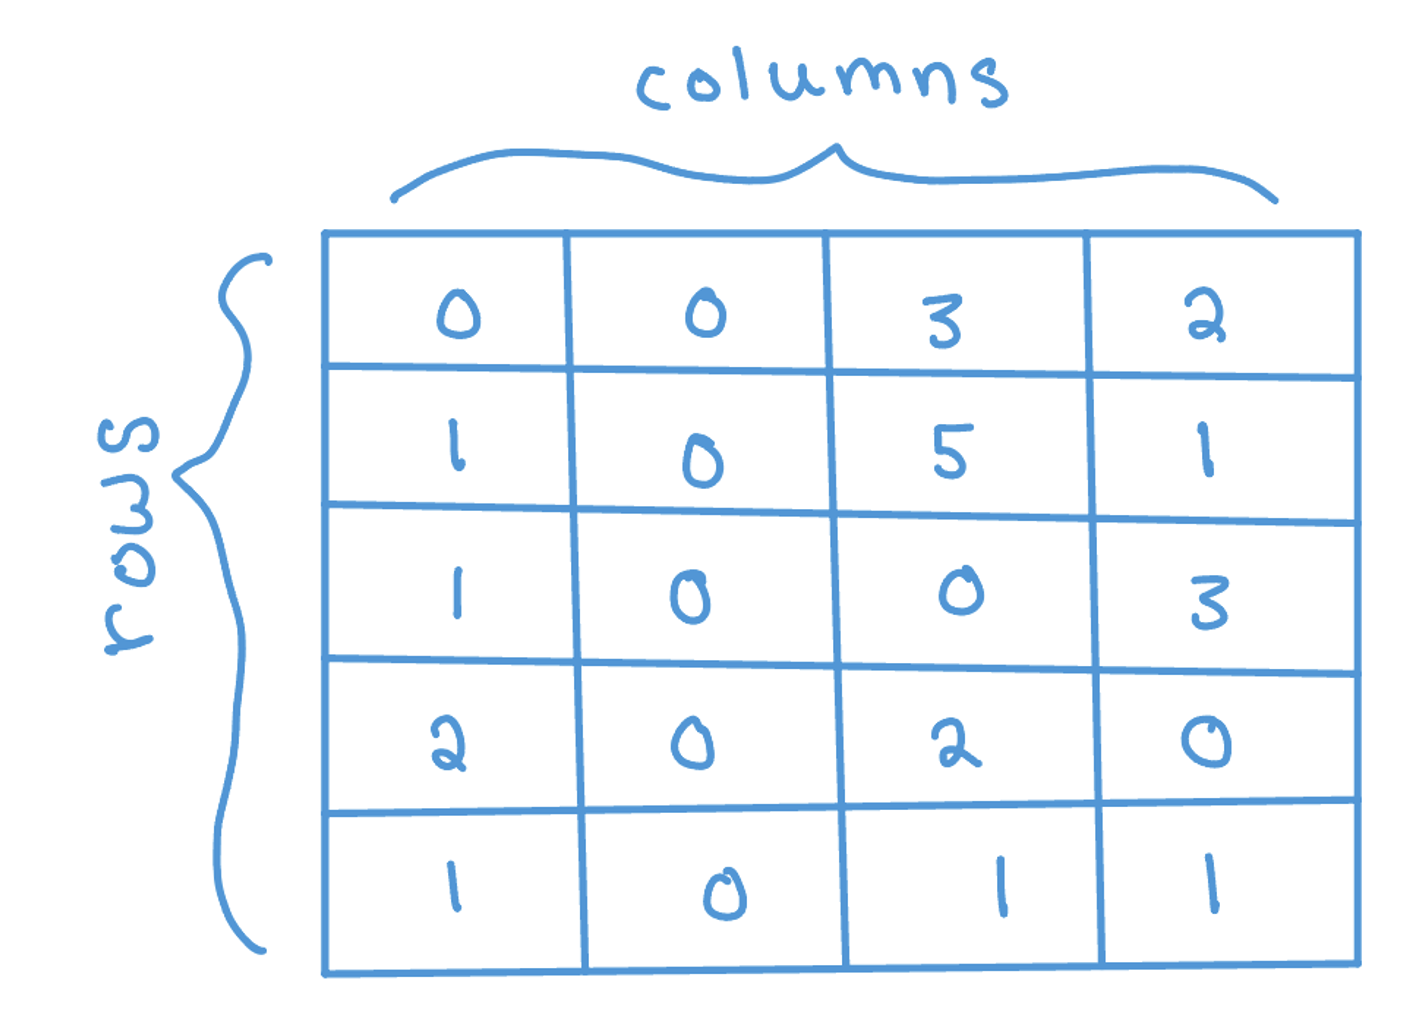
\includegraphics[width=0.4\textwidth,height=\textheight]{book/images/2-matrix.png}

}

\caption{\label{fig-matrix}Matrix Example.}

\end{figure}

Below, we create a matrix reporting the daily rainfall over multiple
weeks. We can create a matrix using the
\texttt{matrix(data,\ nrow,\ ncol,\ byrow)} function. This creates a
\texttt{nrow} by \texttt{ncol} matrix from the vector \texttt{data}
values filling in by row if \texttt{byrow} is TRUE and by column
otherwise. Run the code below. Then, change the last argument to
\texttt{byrow=FALSE} and see what happens to the values.

\begin{Shaded}
\begin{Highlighting}[]
\NormalTok{rainfall }\OtherTok{\textless{}{-}} \FunctionTok{matrix}\NormalTok{(}\FunctionTok{c}\NormalTok{(}\DecValTok{5}\NormalTok{,}\DecValTok{6}\NormalTok{,}\FloatTok{0.1}\NormalTok{,}\DecValTok{3}\NormalTok{,}\DecValTok{0}\NormalTok{,}\DecValTok{1}\NormalTok{,}\DecValTok{0}\NormalTok{,}\DecValTok{1}\NormalTok{,}\FloatTok{0.4}\NormalTok{,}\FloatTok{0.2}\NormalTok{,}\FloatTok{0.5}\NormalTok{,}\FloatTok{0.3}\NormalTok{,}\DecValTok{0}\NormalTok{,}\DecValTok{0}\NormalTok{), }
                   \AttributeTok{ncol=}\DecValTok{7}\NormalTok{, }\AttributeTok{nrow=}\DecValTok{2}\NormalTok{, }\AttributeTok{byrow=}\ConstantTok{TRUE}\NormalTok{)}
\NormalTok{rainfall}
\CommentTok{\#\textgreater{}      [,1] [,2] [,3] [,4] [,5] [,6] [,7]}
\CommentTok{\#\textgreater{} [1,]    5  6.0  0.1  3.0  0.0    1    0}
\CommentTok{\#\textgreater{} [2,]    1  0.4  0.2  0.5  0.3    0    0}
\end{Highlighting}
\end{Shaded}

We can find the dimensions of a matrix using the \texttt{nrow()},
\texttt{ncol()}, or \texttt{dim()} functions, which return the number of
rows, the number of columns, and both the number of rows and columns,
respectively.

\begin{Shaded}
\begin{Highlighting}[]
\FunctionTok{nrow}\NormalTok{(rainfall)}
\CommentTok{\#\textgreater{} [1] 2}
\FunctionTok{ncol}\NormalTok{(rainfall)}
\CommentTok{\#\textgreater{} [1] 7}
\FunctionTok{dim}\NormalTok{(rainfall)}
\CommentTok{\#\textgreater{} [1] 2 7}
\end{Highlighting}
\end{Shaded}

\hypertarget{indexing-a-matrix}{%
\subsection{Indexing a Matrix}\label{indexing-a-matrix}}

Since matrices are two-dimensional, a single value is indexed by both
its row number and its column number. This means that to access a subset
of values in a matrix, we need to provide row and column indices. Below,
we access a single value in the 1st row and the 4th column. The first
value is always the row index and the second value is always the column
index.

\begin{Shaded}
\begin{Highlighting}[]
\NormalTok{rainfall[}\DecValTok{1}\NormalTok{,}\DecValTok{4}\NormalTok{]}
\CommentTok{\#\textgreater{} [1] 3}
\end{Highlighting}
\end{Shaded}

As before, we can also provide multiple indices to get multiple values.
Below, we choose multiple columns but we can also choose multiple rows
(or multiple rows and multiple columns!).

\begin{Shaded}
\begin{Highlighting}[]
\NormalTok{rainfall[}\DecValTok{1}\NormalTok{,}\FunctionTok{c}\NormalTok{(}\DecValTok{4}\NormalTok{,}\DecValTok{5}\NormalTok{,}\DecValTok{7}\NormalTok{)]}
\CommentTok{\#\textgreater{} [1] 3 0 0}
\end{Highlighting}
\end{Shaded}

As with vectors, we can also use booleans to index a matrix by providing
boolean values for the rows and/or columns. Note that below we give a
vector for the row indices and no values for the columns. Since we did
not specify any column indices, this will select all of them.

\begin{Shaded}
\begin{Highlighting}[]
\NormalTok{rainfall[}\FunctionTok{c}\NormalTok{(}\ConstantTok{FALSE}\NormalTok{, }\ConstantTok{TRUE}\NormalTok{), ]}
\CommentTok{\#\textgreater{} [1] 1.0 0.4 0.2 0.5 0.3 0.0 0.0}
\end{Highlighting}
\end{Shaded}

Let's do the opposite and select some columns and all rows.

\begin{Shaded}
\begin{Highlighting}[]
\NormalTok{rainfall[ ,}\FunctionTok{c}\NormalTok{(}\ConstantTok{TRUE}\NormalTok{, }\ConstantTok{TRUE}\NormalTok{, }\ConstantTok{FALSE}\NormalTok{, }\ConstantTok{FALSE}\NormalTok{, }\ConstantTok{FALSE}\NormalTok{, }\ConstantTok{FALSE}\NormalTok{, }\ConstantTok{FALSE}\NormalTok{)]}
\CommentTok{\#\textgreater{}      [,1] [,2]}
\CommentTok{\#\textgreater{} [1,]    5  6.0}
\CommentTok{\#\textgreater{} [2,]    1  0.4}
\end{Highlighting}
\end{Shaded}

As with vectors, we can specify row names and column names to access
entries instead of using indices. The \texttt{colnames()} and
\texttt{rownames()} functions allow us to specify the column and row
names, respectively.

\begin{Shaded}
\begin{Highlighting}[]
\FunctionTok{colnames}\NormalTok{(rainfall) }\OtherTok{\textless{}{-}} \FunctionTok{c}\NormalTok{(}\StringTok{"Monday"}\NormalTok{, }\StringTok{"Tuesday"}\NormalTok{, }\StringTok{"Wednesday"}\NormalTok{, }\StringTok{"Thursday"}\NormalTok{, }
                        \StringTok{"Friday"}\NormalTok{, }\StringTok{"Saturday"}\NormalTok{, }\StringTok{"Sunday"}\NormalTok{)}
\FunctionTok{rownames}\NormalTok{(rainfall) }\OtherTok{\textless{}{-}} \FunctionTok{c}\NormalTok{(}\StringTok{"Week1"}\NormalTok{, }\StringTok{"Week2"}\NormalTok{)}
\NormalTok{rainfall[}\StringTok{"Week1"}\NormalTok{,}\FunctionTok{c}\NormalTok{(}\StringTok{"Friday"}\NormalTok{,}\StringTok{"Saturday"}\NormalTok{)]}
\CommentTok{\#\textgreater{}   Friday Saturday }
\CommentTok{\#\textgreater{}        0        1}
\end{Highlighting}
\end{Shaded}

\hypertarget{editing-a-matrix}{%
\subsection{Editing a Matrix}\label{editing-a-matrix}}

If we want to change the values in a matrix, we need to first index
those values and then assign them the new value(s). Below, we change a
single entry to be 3 and then update several values to all be 0. Note
that we do not provide multiple 0's on the right-hand side, as R will
infer that all values should be set to 0.

\begin{Shaded}
\begin{Highlighting}[]
\NormalTok{rainfall[}\StringTok{"Week1"}\NormalTok{, }\StringTok{"Friday"}\NormalTok{] }\OtherTok{\textless{}{-}} \DecValTok{3}
\end{Highlighting}
\end{Shaded}

\begin{Shaded}
\begin{Highlighting}[]
\NormalTok{rainfall[}\StringTok{"Week1"}\NormalTok{, }\FunctionTok{c}\NormalTok{(}\StringTok{"Monday"}\NormalTok{, }\StringTok{"Tuesday"}\NormalTok{)] }\OtherTok{\textless{}{-}} \DecValTok{0}
\FunctionTok{print}\NormalTok{(rainfall)}
\CommentTok{\#\textgreater{}       Monday Tuesday Wednesday Thursday Friday Saturday Sunday}
\CommentTok{\#\textgreater{} Week1      0     0.0       0.1      3.0    3.0        1      0}
\CommentTok{\#\textgreater{} Week2      1     0.4       0.2      0.5    0.3        0      0}
\end{Highlighting}
\end{Shaded}

Further, we can append values to our matrix by adding rows or columns
through the \texttt{rbind()} and \texttt{cbind()} functions. The first
function appends a row (or multiple rows) to a matrix and the second
appends a column (or multiple columns). Note that below I provide a row
and column name when passing in the additional data. If I hadn't
specified these names, then those rows and columns would not be named.

\begin{Shaded}
\begin{Highlighting}[]
\NormalTok{rainfall }\OtherTok{\textless{}{-}} \FunctionTok{rbind}\NormalTok{(rainfall, }\StringTok{"Week3"} \OtherTok{=} \FunctionTok{c}\NormalTok{(}\FloatTok{0.4}\NormalTok{, }\FloatTok{0.0}\NormalTok{, }\FloatTok{0.0}\NormalTok{, }\FloatTok{0.0}\NormalTok{, }\FloatTok{1.2}\NormalTok{, }\FloatTok{2.2}\NormalTok{, }\FloatTok{0.0}\NormalTok{))}
\NormalTok{rainfall }\OtherTok{\textless{}{-}} \FunctionTok{cbind}\NormalTok{(rainfall, }\StringTok{"Total"} \OtherTok{=} \FunctionTok{c}\NormalTok{(}\FloatTok{7.1}\NormalTok{, }\FloatTok{2.4}\NormalTok{, }\FloatTok{3.8}\NormalTok{))}
\FunctionTok{print}\NormalTok{(rainfall)}
\CommentTok{\#\textgreater{}       Monday Tuesday Wednesday Thursday Friday Saturday Sunday Total}
\CommentTok{\#\textgreater{} Week1    0.0     0.0       0.1      3.0    3.0      1.0      0   7.1}
\CommentTok{\#\textgreater{} Week2    1.0     0.4       0.2      0.5    0.3      0.0      0   2.4}
\CommentTok{\#\textgreater{} Week3    0.4     0.0       0.0      0.0    1.2      2.2      0   3.8}
\end{Highlighting}
\end{Shaded}

Here is an example where we bind two matrices by column. Note that
whenever we bind two matrices together, we have to be sure that their
dimensions are compatible and that they are of the same type.

\begin{Shaded}
\begin{Highlighting}[]
\NormalTok{A }\OtherTok{\textless{}{-}} \FunctionTok{matrix}\NormalTok{(}\FunctionTok{c}\NormalTok{(}\DecValTok{1}\NormalTok{,}\DecValTok{2}\NormalTok{,}\DecValTok{3}\NormalTok{,}\DecValTok{4}\NormalTok{), }\AttributeTok{nrow=}\DecValTok{2}\NormalTok{)}
\NormalTok{B }\OtherTok{\textless{}{-}} \FunctionTok{matrix}\NormalTok{(}\FunctionTok{c}\NormalTok{(}\DecValTok{5}\NormalTok{,}\DecValTok{6}\NormalTok{,}\DecValTok{7}\NormalTok{,}\DecValTok{8}\NormalTok{), }\AttributeTok{nrow=}\DecValTok{2}\NormalTok{)}
\NormalTok{C }\OtherTok{\textless{}{-}} \FunctionTok{cbind}\NormalTok{(A, B)}
\NormalTok{C}
\CommentTok{\#\textgreater{}      [,1] [,2] [,3] [,4]}
\CommentTok{\#\textgreater{} [1,]    1    3    5    7}
\CommentTok{\#\textgreater{} [2,]    2    4    6    8}
\end{Highlighting}
\end{Shaded}

As with vectors, most mathematical operators (\texttt{+}, \texttt{-},
\texttt{*}, \texttt{/} etc.) are applied element-wise in R.

\begin{Shaded}
\begin{Highlighting}[]
\NormalTok{A}\SpecialCharTok{+}\NormalTok{B}
\CommentTok{\#\textgreater{}      [,1] [,2]}
\CommentTok{\#\textgreater{} [1,]    6   10}
\CommentTok{\#\textgreater{} [2,]    8   12}
\end{Highlighting}
\end{Shaded}

\begin{Shaded}
\begin{Highlighting}[]
\FunctionTok{exp}\NormalTok{(C)}
\CommentTok{\#\textgreater{}      [,1] [,2] [,3] [,4]}
\CommentTok{\#\textgreater{} [1,] 2.72 20.1  148 1097}
\CommentTok{\#\textgreater{} [2,] 7.39 54.6  403 2981}
\end{Highlighting}
\end{Shaded}

\hypertarget{practice-question-1}{%
\subsection{Practice Question}\label{practice-question-1}}

Create a 3x4 matrix of all 1's using the \texttt{rep()} and
\texttt{matrix()} functions. Then select the first and third columns
using indexing which will return a 3x2 matrix of all ones.

\begin{Shaded}
\begin{Highlighting}[]
\CommentTok{\# Insert your solution here:}
\end{Highlighting}
\end{Shaded}

\hypertarget{data-frames}{%
\section{Data Frames}\label{data-frames}}

Matrices can store data like the rainfall data, where everything is of
the same type. However, if we want to capture more complex data records,
we also want to allow for different measurement types: this is where
data frames come in. A data frame is like a matrix in that data frames
are two-dimensional, but unlike matrices, data frames allow for each
column to be a different type. In this case, each row corresponds to a
single data entry (or observation) and each column corresponds to a
different variable.

\begin{figure}

{\centering 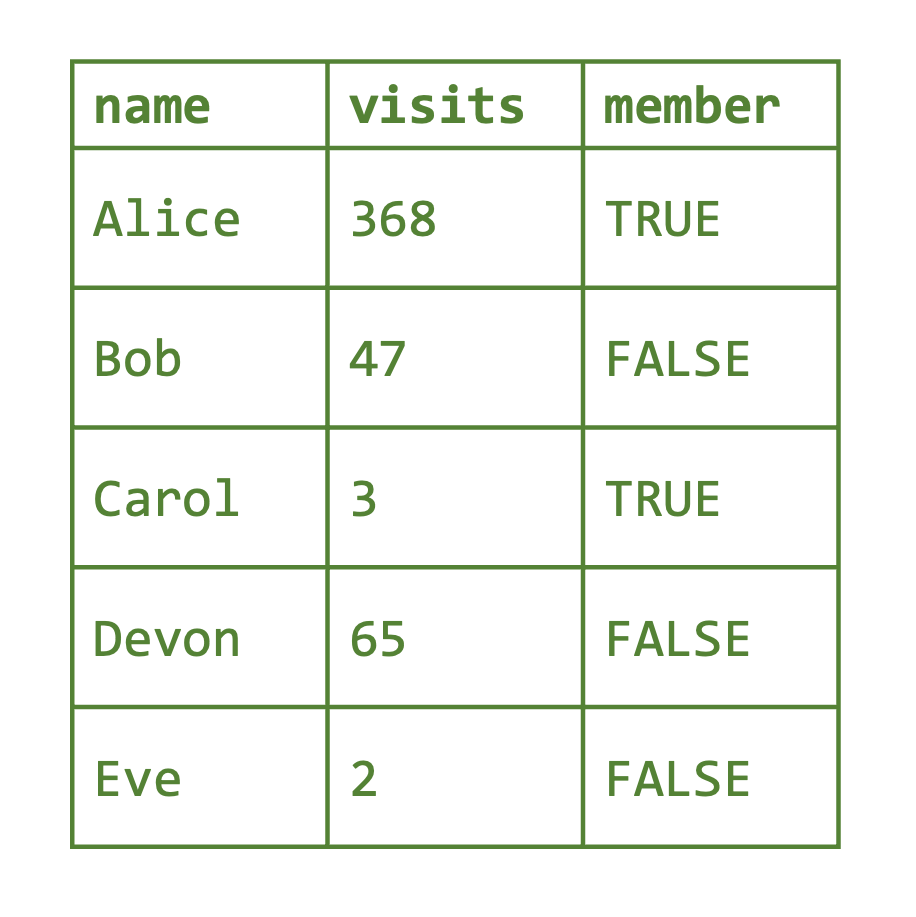
\includegraphics[width=0.3\textwidth,height=\textheight]{book/images/2-dataframe.png}

}

\caption{\label{fig-dataframe}Data Frame Example.}

\end{figure}

For example, suppose that, for every day in a study, we want to record
the temperature, rainfall, and day of the week. Temperature and rainfall
can be numeric values, but day of the week will be character type. We
create a data frame using the \texttt{data.frame()} function. Note that
I am providing column names for each vector (column).

The \texttt{head()} function prints the first six rows of a data frame
(to avoid printing very large datasets). In our case, all the data is
shown because we only created four rows. The column names are displayed
as well as their type. By contrast, the \texttt{tail()} function prints
the last six rows of a data frame.

\begin{Shaded}
\begin{Highlighting}[]
\NormalTok{weather\_data }\OtherTok{\textless{}{-}} \FunctionTok{data.frame}\NormalTok{(}\AttributeTok{day\_of\_week =} \FunctionTok{c}\NormalTok{(}\StringTok{"Monday"}\NormalTok{,}\StringTok{"Tuesday"}\NormalTok{,}\StringTok{"Wednesday"}\NormalTok{,}
                                           \StringTok{"Monday"}\NormalTok{), }
                           \AttributeTok{temp =} \FunctionTok{c}\NormalTok{(}\DecValTok{70}\NormalTok{,}\DecValTok{62}\NormalTok{,}\DecValTok{75}\NormalTok{,}\DecValTok{50}\NormalTok{), }\AttributeTok{rain =} \FunctionTok{c}\NormalTok{(}\DecValTok{5}\NormalTok{,}\FloatTok{0.1}\NormalTok{,}\FloatTok{0.0}\NormalTok{,}\FloatTok{0.5}\NormalTok{))}
\FunctionTok{head}\NormalTok{(weather\_data)}
\CommentTok{\#\textgreater{}   day\_of\_week temp rain}
\CommentTok{\#\textgreater{} 1      Monday   70  5.0}
\CommentTok{\#\textgreater{} 2     Tuesday   62  0.1}
\CommentTok{\#\textgreater{} 3   Wednesday   75  0.0}
\CommentTok{\#\textgreater{} 4      Monday   50  0.5}
\end{Highlighting}
\end{Shaded}

The \texttt{dim()}, \texttt{nrow()}, and \texttt{ncol()} functions
return the dimensions, number of rows, and number of columns of a data
frame, respectively.

\begin{Shaded}
\begin{Highlighting}[]
\FunctionTok{dim}\NormalTok{(weather\_data)}
\CommentTok{\#\textgreater{} [1] 4 3}
\FunctionTok{nrow}\NormalTok{(weather\_data)}
\CommentTok{\#\textgreater{} [1] 4}
\FunctionTok{ncol}\NormalTok{(weather\_data)}
\CommentTok{\#\textgreater{} [1] 3}
\end{Highlighting}
\end{Shaded}

The column names can be found (or assigned) using the
\texttt{colnames()} or \texttt{names()} function. These were specified
when I created the data. On the other hand, the row names are currently
the indices.

\begin{Shaded}
\begin{Highlighting}[]
\FunctionTok{colnames}\NormalTok{(weather\_data)}
\CommentTok{\#\textgreater{} [1] "day\_of\_week" "temp"        "rain"}
\FunctionTok{rownames}\NormalTok{(weather\_data)}
\CommentTok{\#\textgreater{} [1] "1" "2" "3" "4"}
\FunctionTok{names}\NormalTok{(weather\_data)}
\CommentTok{\#\textgreater{} [1] "day\_of\_week" "temp"        "rain"}
\end{Highlighting}
\end{Shaded}

We update the row names to be more informative as with a matrix using
the \texttt{rownames()} function.

\begin{Shaded}
\begin{Highlighting}[]
\FunctionTok{rownames}\NormalTok{(weather\_data) }\OtherTok{\textless{}{-}} \FunctionTok{c}\NormalTok{(}\StringTok{"6/1"}\NormalTok{, }\StringTok{"6/2"}\NormalTok{, }\StringTok{"6/3"}\NormalTok{, }\StringTok{"6/8"}\NormalTok{)}
\FunctionTok{head}\NormalTok{(weather\_data)}
\CommentTok{\#\textgreater{}     day\_of\_week temp rain}
\CommentTok{\#\textgreater{} 6/1      Monday   70  5.0}
\CommentTok{\#\textgreater{} 6/2     Tuesday   62  0.1}
\CommentTok{\#\textgreater{} 6/3   Wednesday   75  0.0}
\CommentTok{\#\textgreater{} 6/8      Monday   50  0.5}
\end{Highlighting}
\end{Shaded}

\hypertarget{indexing-a-data-frame}{%
\subsection{Indexing a Data Frame}\label{indexing-a-data-frame}}

We can select elements of the data frame using its indices in the same
way as we did with matrices. Below, we access a single value and then a
subset of our data frame. The subset returned is itself a data frame.
Note that the second line below returns a data frame.

\begin{Shaded}
\begin{Highlighting}[]
\NormalTok{weather\_data[}\DecValTok{1}\NormalTok{,}\DecValTok{2}\NormalTok{]}
\CommentTok{\#\textgreater{} [1] 70}
\NormalTok{weather\_data[}\DecValTok{1}\NormalTok{,}\FunctionTok{c}\NormalTok{(}\StringTok{"day\_of\_week"}\NormalTok{,}\StringTok{"temp"}\NormalTok{)]}
\CommentTok{\#\textgreater{}     day\_of\_week temp}
\CommentTok{\#\textgreater{} 6/1      Monday   70}
\end{Highlighting}
\end{Shaded}

Another useful way to access the columns of a data frame is by using the
\$ accessor and the column name.

\begin{Shaded}
\begin{Highlighting}[]
\NormalTok{weather\_data}\SpecialCharTok{$}\NormalTok{day\_of\_week}
\CommentTok{\#\textgreater{} [1] "Monday"    "Tuesday"   "Wednesday" "Monday"}
\NormalTok{weather\_data}\SpecialCharTok{$}\NormalTok{temp}
\CommentTok{\#\textgreater{} [1] 70 62 75 50}
\end{Highlighting}
\end{Shaded}

The column \texttt{day\_of\_week} is a categorical column, but it can
only take on a limited number of values. For this kind of column, it is
often useful to convert that column to a factor as we did before.

\begin{Shaded}
\begin{Highlighting}[]
\NormalTok{weather\_data}\SpecialCharTok{$}\NormalTok{day\_of\_week }\OtherTok{\textless{}{-}} \FunctionTok{factor}\NormalTok{(weather\_data}\SpecialCharTok{$}\NormalTok{day\_of\_week)}
\FunctionTok{levels}\NormalTok{(weather\_data}\SpecialCharTok{$}\NormalTok{day\_of\_week)}
\CommentTok{\#\textgreater{} [1] "Monday"    "Tuesday"   "Wednesday"}
\end{Highlighting}
\end{Shaded}

\hypertarget{editing-a-data-frame}{%
\subsection{Editing a Data Frame}\label{editing-a-data-frame}}

As with matrices, we can change values in a data frame by indexing those
entries.

\begin{Shaded}
\begin{Highlighting}[]
\NormalTok{weather\_data[}\DecValTok{1}\NormalTok{, }\StringTok{"rain"}\NormalTok{] }\OtherTok{\textless{}{-}} \FloatTok{2.2}
\NormalTok{weather\_data}
\CommentTok{\#\textgreater{}     day\_of\_week temp rain}
\CommentTok{\#\textgreater{} 6/1      Monday   70  2.2}
\CommentTok{\#\textgreater{} 6/2     Tuesday   62  0.1}
\CommentTok{\#\textgreater{} 6/3   Wednesday   75  0.0}
\CommentTok{\#\textgreater{} 6/8      Monday   50  0.5}
\end{Highlighting}
\end{Shaded}

The \texttt{rbind()} functions and \texttt{cbind()} functions also work
for data frames in the same way as for matrices. However, another way to
add a column is to directly use the \$ accessor. Below, we add a
categorical column called \texttt{aq\_warning}, indicating whether there
was an air quality warning that day.

\begin{Shaded}
\begin{Highlighting}[]
\NormalTok{weather\_data}\SpecialCharTok{$}\NormalTok{aq\_warning }\OtherTok{\textless{}{-}} \FunctionTok{as.factor}\NormalTok{(}\FunctionTok{c}\NormalTok{(}\DecValTok{1}\NormalTok{, }\DecValTok{0}\NormalTok{, }\DecValTok{0}\NormalTok{, }\DecValTok{0}\NormalTok{))}
\NormalTok{weather\_data}
\CommentTok{\#\textgreater{}     day\_of\_week temp rain aq\_warning}
\CommentTok{\#\textgreater{} 6/1      Monday   70  2.2          1}
\CommentTok{\#\textgreater{} 6/2     Tuesday   62  0.1          0}
\CommentTok{\#\textgreater{} 6/3   Wednesday   75  0.0          0}
\CommentTok{\#\textgreater{} 6/8      Monday   50  0.5          0}
\end{Highlighting}
\end{Shaded}

\hypertarget{practice-question-2}{%
\subsection{Practice Question}\label{practice-question-2}}

Add a column to \texttt{weather\_data} called
\texttt{air\_quality\_index} using the \texttt{rep()} function so that
all values are \texttt{NA} (the missing value in R). Then, index the
second value of this column and set the value to be 57. The result
should look like Figure~\ref{fig-practice-question}.

\begin{figure}

{\centering 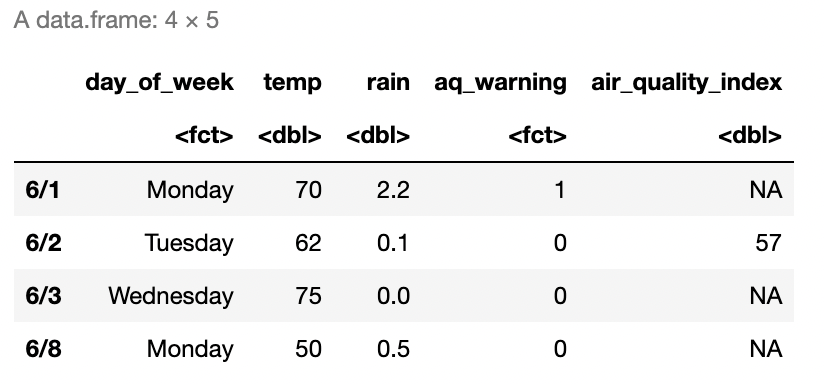
\includegraphics[width=0.7\textwidth,height=\textheight]{book/images/2-practicequestionanswer.png}

}

\caption{\label{fig-practice-question}Air Quality Data.}

\end{figure}

\begin{Shaded}
\begin{Highlighting}[]
\CommentTok{\# Insert your solution here:}
\end{Highlighting}
\end{Shaded}

\hypertarget{lists}{%
\section{Lists}\label{lists}}

A data frame is actually a special kind of another data structure called
a \textbf{list}, which is a collection of objects under the same name.
These objects can be vectors, matrices, data frames, or even other
lists! There does not have to be any relation in size, type, or other
attribute between different members of the list. Below, we create an
example list using the \texttt{list()} function, which takes in a series
of objects. What are the types of each element of the list? We can
access each element using the index, but here we need to use double
brackets.

\begin{Shaded}
\begin{Highlighting}[]
\NormalTok{ex\_list }\OtherTok{\textless{}{-}} \FunctionTok{list}\NormalTok{(}\StringTok{"John"}\NormalTok{, }\FunctionTok{c}\NormalTok{(}\StringTok{"ibuprofen"}\NormalTok{, }\StringTok{"metformin"}\NormalTok{), }\FunctionTok{c}\NormalTok{(}\DecValTok{136}\NormalTok{, }\DecValTok{142}\NormalTok{, }\DecValTok{159}\NormalTok{))}
\FunctionTok{print}\NormalTok{(ex\_list)}
\CommentTok{\#\textgreater{} [[1]]}
\CommentTok{\#\textgreater{} [1] "John"}
\CommentTok{\#\textgreater{} }
\CommentTok{\#\textgreater{} [[2]]}
\CommentTok{\#\textgreater{} [1] "ibuprofen" "metformin"}
\CommentTok{\#\textgreater{} }
\CommentTok{\#\textgreater{} [[3]]}
\CommentTok{\#\textgreater{} [1] 136 142 159}
\NormalTok{ex\_list[[}\DecValTok{2}\NormalTok{]]}
\CommentTok{\#\textgreater{} [1] "ibuprofen" "metformin"}
\end{Highlighting}
\end{Shaded}

More often, however, it is useful to name the elements of the list for
easier access. Let's create this list again but this time give names to
each object.

\begin{Shaded}
\begin{Highlighting}[]
\NormalTok{ex\_list }\OtherTok{\textless{}{-}} \FunctionTok{list}\NormalTok{(}\AttributeTok{name=}\StringTok{"John"}\NormalTok{, }\AttributeTok{medications =} \FunctionTok{c}\NormalTok{(}\StringTok{"ibuprofen"}\NormalTok{, }\StringTok{"metformin"}\NormalTok{), }
                \AttributeTok{past\_weights =} \FunctionTok{c}\NormalTok{(}\DecValTok{136}\NormalTok{, }\DecValTok{142}\NormalTok{, }\DecValTok{159}\NormalTok{))}
\FunctionTok{print}\NormalTok{(ex\_list)}
\CommentTok{\#\textgreater{} $name}
\CommentTok{\#\textgreater{} [1] "John"}
\CommentTok{\#\textgreater{} }
\CommentTok{\#\textgreater{} $medications}
\CommentTok{\#\textgreater{} [1] "ibuprofen" "metformin"}
\CommentTok{\#\textgreater{} }
\CommentTok{\#\textgreater{} $past\_weights}
\CommentTok{\#\textgreater{} [1] 136 142 159}
\NormalTok{ex\_list}\SpecialCharTok{$}\NormalTok{medications}
\CommentTok{\#\textgreater{} [1] "ibuprofen" "metformin"}
\end{Highlighting}
\end{Shaded}

To edit a list, we can use indexing to access different objects in the
list and then assign them to new values. Additionally, we can add
objects to the list using the \$ accessor.

\begin{Shaded}
\begin{Highlighting}[]
\NormalTok{ex\_list}\SpecialCharTok{$}\NormalTok{supplements }\OtherTok{\textless{}{-}} \FunctionTok{c}\NormalTok{(}\StringTok{"vitamin D"}\NormalTok{, }\StringTok{"biotin"}\NormalTok{)}
\NormalTok{ex\_list}\SpecialCharTok{$}\NormalTok{supplements[}\DecValTok{2}\NormalTok{] }\OtherTok{\textless{}{-}} \StringTok{"collagen"}
\NormalTok{ex\_list}
\CommentTok{\#\textgreater{} $name}
\CommentTok{\#\textgreater{} [1] "John"}
\CommentTok{\#\textgreater{} }
\CommentTok{\#\textgreater{} $medications}
\CommentTok{\#\textgreater{} [1] "ibuprofen" "metformin"}
\CommentTok{\#\textgreater{} }
\CommentTok{\#\textgreater{} $past\_weights}
\CommentTok{\#\textgreater{} [1] 136 142 159}
\CommentTok{\#\textgreater{} }
\CommentTok{\#\textgreater{} $supplements}
\CommentTok{\#\textgreater{} [1] "vitamin D" "collagen"}
\end{Highlighting}
\end{Shaded}

\hypertarget{exercises}{%
\section{Exercises}\label{exercises}}

\begin{enumerate}
\def\labelenumi{\arabic{enumi}.}
\tightlist
\item
  Recreate the data frame in Figure~\ref{fig-city-air-quality} in R,
  where \texttt{temperature} and \texttt{co2} represent the average
  temperature in Fahrenheit and the average \(\text{CO}_2\)
  concentrations in \(\text{mg}/\text{m}^3\) for the month of January
  2008, and name it \texttt{city\_air\_quality}.
\end{enumerate}

\begin{figure}

{\centering 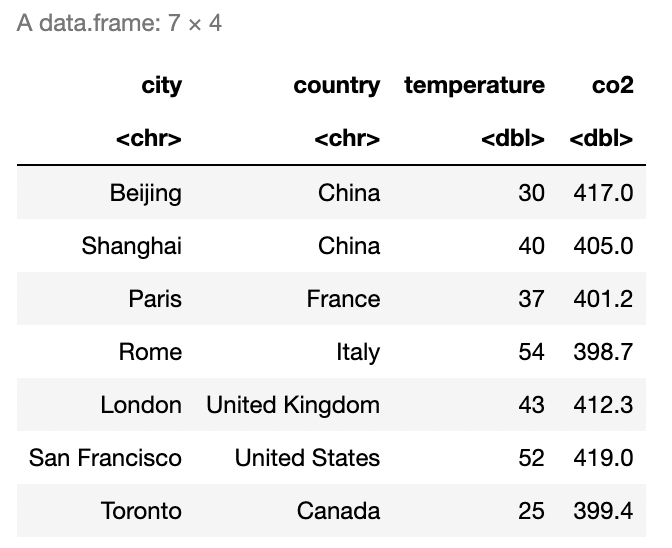
\includegraphics[width=0.7\textwidth,height=\textheight]{book/images/2-exercise1df.png}

}

\caption{\label{fig-city-air-quality}City Air Quality Data.}

\end{figure}

\begin{enumerate}
\def\labelenumi{\arabic{enumi}.}
\setcounter{enumi}{1}
\item
  Create a character vector named \texttt{precipitation} with entries
  \texttt{Yes} or \texttt{No} indicating whether or not there was more
  precipitation than average in January 2008 in these cities (you can
  make this information up yourself). Then, append this vector to the
  \texttt{city\_air\_quality} data frame as a new column.
\item
  Convert the categorical column \texttt{precipitation} to a factor.
  Then, add a row to the data frame \texttt{city\_air\_quality} using
  the \texttt{rbind()} function to match
  Figure~\ref{fig-city-air-quality-2}.
\end{enumerate}

\begin{figure}

{\centering 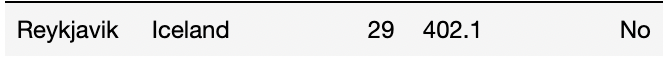
\includegraphics[width=0.5\textwidth,height=\textheight]{book/images/2-exercise3newrow.png}

}

\caption{\label{fig-city-air-quality-2}Updated City Air Quality Data.}

\end{figure}

\begin{enumerate}
\def\labelenumi{\arabic{enumi}.}
\setcounter{enumi}{3}
\tightlist
\item
  Use single square brackets to access the precipitation and
  \(\text{CO}_2\) concentration entries for San Francisco and Paris in
  your data frame. Then, create a list \texttt{city\_list} which
  contains two lists, one for San Francisco and one for Paris, where
  each inner list contains the city name, precipitation, and
  \(\text{CO}_2\) concentration information for that city.
\end{enumerate}

\bookmarksetup{startatroot}

\hypertarget{sec-data-files}{%
\chapter{Working with Data Files in R}\label{sec-data-files}}

In this chapter, we will be working with data in R. To start, we need to
load our data into R: this requires identifying the type of data file we
have (e.g.~.csv, .xlsx, .dta) and finding the appropriate function to
load in the data. This will create a data frame object containing the
information from the file. After demonstrating how to load in such data,
this chapter will show you how to find information about data columns,
including finding missing values, summarizing columns, and subsetting
the data. Additionally, we look at how to create new columns through
some simple transformations.

In this chapter and all future chapters, we will load in the required
libraries at the start of the chapter - for example, in this particular
chapter, we need a single package \textbf{HDSinRdata} that contains the
sample data sets used in this book.

\begin{Shaded}
\begin{Highlighting}[]
\FunctionTok{library}\NormalTok{(HDSinRdata)}
\end{Highlighting}
\end{Shaded}

\hypertarget{importing-and-exporting-data}{%
\section{Importing and Exporting
Data}\label{importing-and-exporting-data}}

The data we will use in this chapter contains information about patients
who visited one of the University of Pittsburgh's seven pain management
clinics. This includes patient-reported pain assessments using the
Collaborative Health Outcomes Information Registry (CHOIR) at baseline
and at a 3-month follow-up (Alter et al. 2021). You can use the help
operator \texttt{?pain} to learn more about the source of this data and
to read its column descriptions. Since this data is available in our R
package, we can use the \texttt{data()} function to load this data into
our environment. Note that this data has 21,659 rows and 92 columns.

\begin{Shaded}
\begin{Highlighting}[]
\FunctionTok{data}\NormalTok{(pain)}
\FunctionTok{dim}\NormalTok{(pain)}
\CommentTok{\#\textgreater{} [1] 21659    92}
\end{Highlighting}
\end{Shaded}

In general, the data you will be using will not be available in R
packages and will instead exist in one or more data files on your
personal computer. In order to load in this data to R, you need to use
the function that corresponds to the file type you have. For example,
you can load a .csv file using the \texttt{read.csv()} function in base
R or using the \texttt{read\_csv()} function from the \texttt{readr}
package (Wickham, Hester, and Bryan 2023), both of which were shown in
Chapter~\ref{sec-intro-to-r}. As an example, we load the
\texttt{fake\_names.csv} dataset below using both of these functions:
looking at the print output below, we can see that there is slight
difference in the data structure and data types storing the data between
these two functions. The function \texttt{read.csv()} loads the data as
a data frame, whereas the function \texttt{read\_csv()} loads the data
as a \texttt{spec\_tbl\_df}, a special type of data frame called a
\textbf{tibble} that is used by the \textbf{tidyverse} packages. We will
cover this data structure in more detail in
Chapter~\ref{sec-transformations-summaries}. For now, note that you can
use either function to read in a .csv file.

\begin{Shaded}
\begin{Highlighting}[]
\FunctionTok{read.csv}\NormalTok{(}\StringTok{"data/fake\_names.csv"}\NormalTok{)}
\CommentTok{\#\textgreater{}                  Name Age     DOB            City State}
\CommentTok{\#\textgreater{} 1           Ken Irwin  37 6/28/85      Providence    RI}
\CommentTok{\#\textgreater{} 2 Delores Whittington  56 4/28/67      Smithfield    RI}
\CommentTok{\#\textgreater{} 3       Daniel Hughes  41 5/22/82      Providence    RI}
\CommentTok{\#\textgreater{} 4         Carlos Fain  83  2/2/40          Warren    RI}
\CommentTok{\#\textgreater{} 5        James Alford  67 2/23/56 East Providence    RI}
\CommentTok{\#\textgreater{} 6        Ruth Alvarez  34 9/22/88      Providence    RI}
\end{Highlighting}
\end{Shaded}

\begin{Shaded}
\begin{Highlighting}[]
\NormalTok{readr}\SpecialCharTok{::}\FunctionTok{read\_csv}\NormalTok{(}\StringTok{"data/fake\_names.csv"}\NormalTok{, }\AttributeTok{show\_col\_types=}\ConstantTok{FALSE}\NormalTok{)}
\CommentTok{\#\textgreater{} \# A tibble: 6 x 5}
\CommentTok{\#\textgreater{}   Name                  Age DOB     City            State}
\CommentTok{\#\textgreater{}   \textless{}chr\textgreater{}               \textless{}dbl\textgreater{} \textless{}chr\textgreater{}   \textless{}chr\textgreater{}           \textless{}chr\textgreater{}}
\CommentTok{\#\textgreater{} 1 Ken Irwin              37 6/28/85 Providence      RI   }
\CommentTok{\#\textgreater{} 2 Delores Whittington    56 4/28/67 Smithfield      RI   }
\CommentTok{\#\textgreater{} 3 Daniel Hughes          41 5/22/82 Providence      RI   }
\CommentTok{\#\textgreater{} 4 Carlos Fain            83 2/2/40  Warren          RI   }
\CommentTok{\#\textgreater{} 5 James Alford           67 2/23/56 East Providence RI   }
\CommentTok{\#\textgreater{} \# i 1 more row}
\end{Highlighting}
\end{Shaded}

In addition to loading data into R, you may also want to save data from
R into a data file you can access later or share with others. To write a
data frame from R to a .csv file, you can use the \texttt{write.csv()}
function. This function has three key arguments: the first argument is
the data frame in R that you want to write to a file, the second
argument is the file name or the full file path where you want to write
the data, and the third argument is whether or not you want to include
the row names as an extra column. In this case, we will not include row
names. If you do not specify a file path, R will save the file in our
current working directory.

\begin{Shaded}
\begin{Highlighting}[]
\NormalTok{df }\OtherTok{\textless{}{-}} \FunctionTok{data.frame}\NormalTok{(}\AttributeTok{x=}\FunctionTok{c}\NormalTok{(}\DecValTok{1}\NormalTok{,}\DecValTok{0}\NormalTok{,}\DecValTok{1}\NormalTok{), }\AttributeTok{y=}\FunctionTok{c}\NormalTok{(}\StringTok{"A"}\NormalTok{, }\StringTok{"B"}\NormalTok{, }\StringTok{"C"}\NormalTok{))}
\FunctionTok{write.csv}\NormalTok{(df, }\StringTok{"data/test.csv"}\NormalTok{, }\AttributeTok{row.names=}\ConstantTok{FALSE}\NormalTok{)}
\end{Highlighting}
\end{Shaded}

If your data is not in a .csv file, you may need to use another package
to read in the file. The two most common packages are the
\textbf{readxl} package (Wickham and Bryan 2023), which makes it easy to
read in Excel files, and the \textbf{haven} package (Wickham, Miller,
and Smith 2023), which can import SAS, SPSS, and Stata files. For each
function, you need to specify the file path to the data file.

\begin{itemize}
\item
  \textbf{Excel Files}: You can read in a .xls or .xlsx file using
  \texttt{readxl::read\_excel()}, which allows you to specify a sheet
  and/or cell range within a file.
  (e.g.~\texttt{read\_excel(\textquotesingle{}test.xlsx\textquotesingle{},\ sheet="Sheet1")})
\item
  \textbf{SAS}: \texttt{haven::read\_sas()} reads in .sas7bdat or
  .sas7bcat files, \texttt{haven::read\_xpt()} reads in SAS transport
  files
\item
  \textbf{Stata}: \texttt{haven::read\_dta()} reads in .dta files
\item
  \textbf{SPSS}: \texttt{haven::read\_spss()} reads in .spss files
\end{itemize}

\hypertarget{summarizing-and-creating-data-columns}{%
\section{Summarizing and Creating Data
Columns}\label{summarizing-and-creating-data-columns}}

We will now look at the data we have loaded into the data frame called
\texttt{pain}. We use the \texttt{head()} function to print the first
six rows. However, note that we have so many columns that all not of the
columns are displayed! For those that are displayed, we can see the data
type for each column under the column name. For example, we can see that
the column \texttt{PATIENT\_NUM} is a numeric column of type
\texttt{dbl}. Because patients identification numbers are technically
nominal in nature, we might consider whether we should make convert this
column to a factor or a character representation later on. We can use
the \texttt{names()} function to print all the column names. Note that
columns \texttt{X101} to \texttt{X238} correspond to numbers on a body
pain map (see the data documentation for the image of this map). Each of
these columns has a 1 if the patient indicated that they have pain in
that corresponding body part and a 0 otherwise.

\begin{Shaded}
\begin{Highlighting}[]
\FunctionTok{head}\NormalTok{(pain)}
\CommentTok{\#\textgreater{} \# A tibble: 6 x 92}
\CommentTok{\#\textgreater{}   PATIENT\_NUM  X101  X102  X103  X104  X105  X106  X107  X108  X109  X110  X111}
\CommentTok{\#\textgreater{}         \textless{}dbl\textgreater{} \textless{}dbl\textgreater{} \textless{}dbl\textgreater{} \textless{}dbl\textgreater{} \textless{}dbl\textgreater{} \textless{}dbl\textgreater{} \textless{}dbl\textgreater{} \textless{}dbl\textgreater{} \textless{}dbl\textgreater{} \textless{}dbl\textgreater{} \textless{}dbl\textgreater{} \textless{}dbl\textgreater{}}
\CommentTok{\#\textgreater{} 1       13118     0     0     0     0     0     0     0     0     0     0     0}
\CommentTok{\#\textgreater{} 2       21384     0     0     0     0     0     0     0     0     0     0     0}
\CommentTok{\#\textgreater{} 3        6240     0     0     0     0     0     0     0     0     0     0     0}
\CommentTok{\#\textgreater{} 4        1827     0     0     0     0     0     0     0     0     0     0     0}
\CommentTok{\#\textgreater{} 5       11309     0     0     0     0     0     0     0     0     0     0     0}
\CommentTok{\#\textgreater{} \# i 1 more row}
\CommentTok{\#\textgreater{} \# i 80 more variables: X112 \textless{}dbl\textgreater{}, X113 \textless{}dbl\textgreater{}, X114 \textless{}dbl\textgreater{}, X115 \textless{}dbl\textgreater{},}
\CommentTok{\#\textgreater{} \#   X116 \textless{}dbl\textgreater{}, X117 \textless{}dbl\textgreater{}, X118 \textless{}dbl\textgreater{}, X119 \textless{}dbl\textgreater{}, X120 \textless{}dbl\textgreater{}, X121 \textless{}dbl\textgreater{},}
\CommentTok{\#\textgreater{} \#   X122 \textless{}dbl\textgreater{}, X123 \textless{}dbl\textgreater{}, X124 \textless{}dbl\textgreater{}, X125 \textless{}dbl\textgreater{}, X126 \textless{}dbl\textgreater{}, X127 \textless{}dbl\textgreater{},}
\CommentTok{\#\textgreater{} \#   X128 \textless{}dbl\textgreater{}, X129 \textless{}dbl\textgreater{}, X130 \textless{}dbl\textgreater{}, X131 \textless{}dbl\textgreater{}, X132 \textless{}dbl\textgreater{}, X133 \textless{}dbl\textgreater{},}
\CommentTok{\#\textgreater{} \#   X134 \textless{}dbl\textgreater{}, X135 \textless{}dbl\textgreater{}, X136 \textless{}dbl\textgreater{}, X201 \textless{}dbl\textgreater{}, X202 \textless{}dbl\textgreater{}, X203 \textless{}dbl\textgreater{},}
\CommentTok{\#\textgreater{} \#   X204 \textless{}dbl\textgreater{}, X205 \textless{}dbl\textgreater{}, X206 \textless{}dbl\textgreater{}, X207 \textless{}dbl\textgreater{}, X208 \textless{}dbl\textgreater{}, X209 \textless{}dbl\textgreater{}, ...}
\FunctionTok{names}\NormalTok{(pain)}
\CommentTok{\#\textgreater{}  [1] "PATIENT\_NUM"                      "X101"                            }
\CommentTok{\#\textgreater{}  [3] "X102"                             "X103"                            }
\CommentTok{\#\textgreater{}  [5] "X104"                             "X105"                            }
\CommentTok{\#\textgreater{}  [7] "X106"                             "X107"                            }
\CommentTok{\#\textgreater{}  [9] "X108"                             "X109"                            }
\CommentTok{\#\textgreater{} [11] "X110"                             "X111"                            }
\CommentTok{\#\textgreater{} [13] "X112"                             "X113"                            }
\CommentTok{\#\textgreater{} [15] "X114"                             "X115"                            }
\CommentTok{\#\textgreater{} [17] "X116"                             "X117"                            }
\CommentTok{\#\textgreater{} [19] "X118"                             "X119"                            }
\CommentTok{\#\textgreater{} [21] "X120"                             "X121"                            }
\CommentTok{\#\textgreater{} [23] "X122"                             "X123"                            }
\CommentTok{\#\textgreater{} [25] "X124"                             "X125"                            }
\CommentTok{\#\textgreater{} [27] "X126"                             "X127"                            }
\CommentTok{\#\textgreater{} [29] "X128"                             "X129"                            }
\CommentTok{\#\textgreater{} [31] "X130"                             "X131"                            }
\CommentTok{\#\textgreater{} [33] "X132"                             "X133"                            }
\CommentTok{\#\textgreater{} [35] "X134"                             "X135"                            }
\CommentTok{\#\textgreater{} [37] "X136"                             "X201"                            }
\CommentTok{\#\textgreater{} [39] "X202"                             "X203"                            }
\CommentTok{\#\textgreater{} [41] "X204"                             "X205"                            }
\CommentTok{\#\textgreater{} [43] "X206"                             "X207"                            }
\CommentTok{\#\textgreater{} [45] "X208"                             "X209"                            }
\CommentTok{\#\textgreater{} [47] "X210"                             "X211"                            }
\CommentTok{\#\textgreater{} [49] "X212"                             "X213"                            }
\CommentTok{\#\textgreater{} [51] "X214"                             "X215"                            }
\CommentTok{\#\textgreater{} [53] "X216"                             "X217"                            }
\CommentTok{\#\textgreater{} [55] "X218"                             "X219"                            }
\CommentTok{\#\textgreater{} [57] "X220"                             "X221"                            }
\CommentTok{\#\textgreater{} [59] "X222"                             "X223"                            }
\CommentTok{\#\textgreater{} [61] "X224"                             "X225"                            }
\CommentTok{\#\textgreater{} [63] "X226"                             "X227"                            }
\CommentTok{\#\textgreater{} [65] "X228"                             "X229"                            }
\CommentTok{\#\textgreater{} [67] "X230"                             "X231"                            }
\CommentTok{\#\textgreater{} [69] "X232"                             "X233"                            }
\CommentTok{\#\textgreater{} [71] "X234"                             "X235"                            }
\CommentTok{\#\textgreater{} [73] "X236"                             "X237"                            }
\CommentTok{\#\textgreater{} [75] "X238"                             "PAIN\_INTENSITY\_AVERAGE"          }
\CommentTok{\#\textgreater{} [77] "PROMIS\_PHYSICAL\_FUNCTION"         "PROMIS\_PAIN\_BEHAVIOR"            }
\CommentTok{\#\textgreater{} [79] "PROMIS\_DEPRESSION"                "PROMIS\_ANXIETY"                  }
\CommentTok{\#\textgreater{} [81] "PROMIS\_SLEEP\_DISTURB\_V1\_0"        "PROMIS\_PAIN\_INTERFERENCE"        }
\CommentTok{\#\textgreater{} [83] "GH\_MENTAL\_SCORE"                  "GH\_PHYSICAL\_SCORE"               }
\CommentTok{\#\textgreater{} [85] "AGE\_AT\_CONTACT"                   "BMI"                             }
\CommentTok{\#\textgreater{} [87] "CCI\_TOTAL\_SCORE"                  "PAIN\_INTENSITY\_AVERAGE.FOLLOW\_UP"}
\CommentTok{\#\textgreater{} [89] "PAT\_SEX"                          "PAT\_RACE"                        }
\CommentTok{\#\textgreater{} [91] "CCI\_BIN"                          "MEDICAID\_BIN"}
\end{Highlighting}
\end{Shaded}

Recall that the \texttt{\$} operator can be used to access a single
column. Alternatively, we can use double brackets \texttt{{[}{[}{]}{]}}
to select a column. Below, we demonstrate both ways to print the first
five values in the column with the patient's average pain intensity.

\begin{Shaded}
\begin{Highlighting}[]
\NormalTok{pain}\SpecialCharTok{$}\NormalTok{PAIN\_INTENSITY\_AVERAGE[}\DecValTok{1}\SpecialCharTok{:}\DecValTok{5}\NormalTok{]}
\CommentTok{\#\textgreater{} [1] 7 5 4 7 8}
\NormalTok{pain[[}\StringTok{"PAIN\_INTENSITY\_AVERAGE"}\NormalTok{]][}\DecValTok{1}\SpecialCharTok{:}\DecValTok{5}\NormalTok{]}
\CommentTok{\#\textgreater{} [1] 7 5 4 7 8}
\end{Highlighting}
\end{Shaded}

\hypertarget{column-summaries}{%
\subsection{Column Summaries}\label{column-summaries}}

To explore the range and distribution of a column's values, we can use
some of the base R functions. For example, the \texttt{summary()}
function is a useful way to summarize a numeric column's values. Below,
we can see that the pain intensity values range from 0 to 10 with a
median value of 7 and that there is 1 NA value.

\begin{Shaded}
\begin{Highlighting}[]
\FunctionTok{summary}\NormalTok{(pain}\SpecialCharTok{$}\NormalTok{PAIN\_INTENSITY\_AVERAGE)}
\CommentTok{\#\textgreater{}    Min. 1st Qu.  Median    Mean 3rd Qu.    Max.    NA\textquotesingle{}s }
\CommentTok{\#\textgreater{}    0.00    5.00    7.00    6.49    8.00   10.00       1}
\end{Highlighting}
\end{Shaded}

We have already seen the \texttt{max()}, \texttt{min()},
\texttt{mean()}, and \texttt{median()} functions that could have
computed some of these values for us separately. Since we do have an NA
value, we add the \texttt{na.rm=TRUE} argument to these functions.
Without this argument, the returned value for all of the functions will
be NA.

\begin{Shaded}
\begin{Highlighting}[]
\FunctionTok{min}\NormalTok{(pain}\SpecialCharTok{$}\NormalTok{PAIN\_INTENSITY\_AVERAGE, }\AttributeTok{na.rm=}\ConstantTok{TRUE}\NormalTok{)}
\CommentTok{\#\textgreater{} [1] 0}
\FunctionTok{max}\NormalTok{(pain}\SpecialCharTok{$}\NormalTok{PAIN\_INTENSITY\_AVERAGE, }\AttributeTok{na.rm=}\ConstantTok{TRUE}\NormalTok{)}
\CommentTok{\#\textgreater{} [1] 10}
\FunctionTok{mean}\NormalTok{(pain}\SpecialCharTok{$}\NormalTok{PAIN\_INTENSITY\_AVERAGE, }\AttributeTok{na.rm=}\ConstantTok{TRUE}\NormalTok{)}
\CommentTok{\#\textgreater{} [1] 6.49}
\FunctionTok{median}\NormalTok{(pain}\SpecialCharTok{$}\NormalTok{PAIN\_INTENSITY\_AVERAGE, }\AttributeTok{na.rm=}\ConstantTok{TRUE}\NormalTok{)}
\CommentTok{\#\textgreater{} [1] 7}
\end{Highlighting}
\end{Shaded}

Additionally, the functions below are helpful for summarizing
quantitative columns.

\begin{itemize}
\tightlist
\item
  \texttt{range()} - returns the minimum and maximum values for a
  numeric vector x
\item
  \texttt{quantile()} - returns the sample quantiles for a numeric
  vector
\item
  \texttt{IQR()} - returns the interquartile range for a numeric vector
\end{itemize}

By default, the \texttt{quantile()} function returns the sample
quantiles.

\begin{Shaded}
\begin{Highlighting}[]
\FunctionTok{quantile}\NormalTok{(pain}\SpecialCharTok{$}\NormalTok{PAIN\_INTENSITY\_AVERAGE, }\AttributeTok{na.rm =} \ConstantTok{TRUE}\NormalTok{)}
\CommentTok{\#\textgreater{}   0\%  25\%  50\%  75\% 100\% }
\CommentTok{\#\textgreater{}    0    5    7    8   10}
\end{Highlighting}
\end{Shaded}

However, we can pass in a list of probabilities to use instead. For
example, below we find the 0.1 and 0.9 quantiles. Again, we add the
\texttt{na.rm=TRUE} argument.

\begin{Shaded}
\begin{Highlighting}[]
\FunctionTok{quantile}\NormalTok{(pain}\SpecialCharTok{$}\NormalTok{PAIN\_INTENSITY\_AVERAGE, }\AttributeTok{probs =} \FunctionTok{c}\NormalTok{(}\FloatTok{0.1}\NormalTok{, }\FloatTok{0.9}\NormalTok{), }\AttributeTok{na.rm=}\ConstantTok{TRUE}\NormalTok{)}
\CommentTok{\#\textgreater{} 10\% 90\% }
\CommentTok{\#\textgreater{}   4   9}
\end{Highlighting}
\end{Shaded}

We can also plot a histogram of the sample distribution using the
\texttt{hist()} function. We will look more in depth at how to change
aspects of this histogram in Chapter~\ref{sec-exploratory}.

\begin{Shaded}
\begin{Highlighting}[]
\FunctionTok{hist}\NormalTok{(pain}\SpecialCharTok{$}\NormalTok{PAIN\_INTENSITY\_AVERAGE)}
\end{Highlighting}
\end{Shaded}

\begin{figure}[H]

{\centering 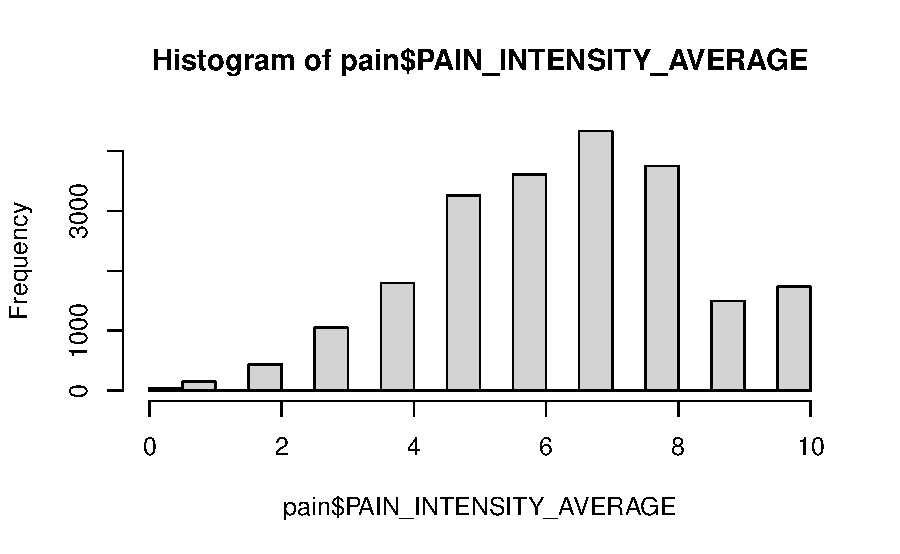
\includegraphics[width=1\textwidth,height=\textheight]{book/3_data_files_files/figure-pdf/unnamed-chunk-12-1.pdf}

}

\end{figure}

\hypertarget{practice-question-3}{%
\subsection{Practice Question}\label{practice-question-3}}

Summarize the \texttt{PROMIS\_SLEEP\_DISTURB\_V1\_0} column both
numerically and visually. Your results should look like the results in
Figure~\ref{fig-pq1}.

\begin{figure}

{\centering 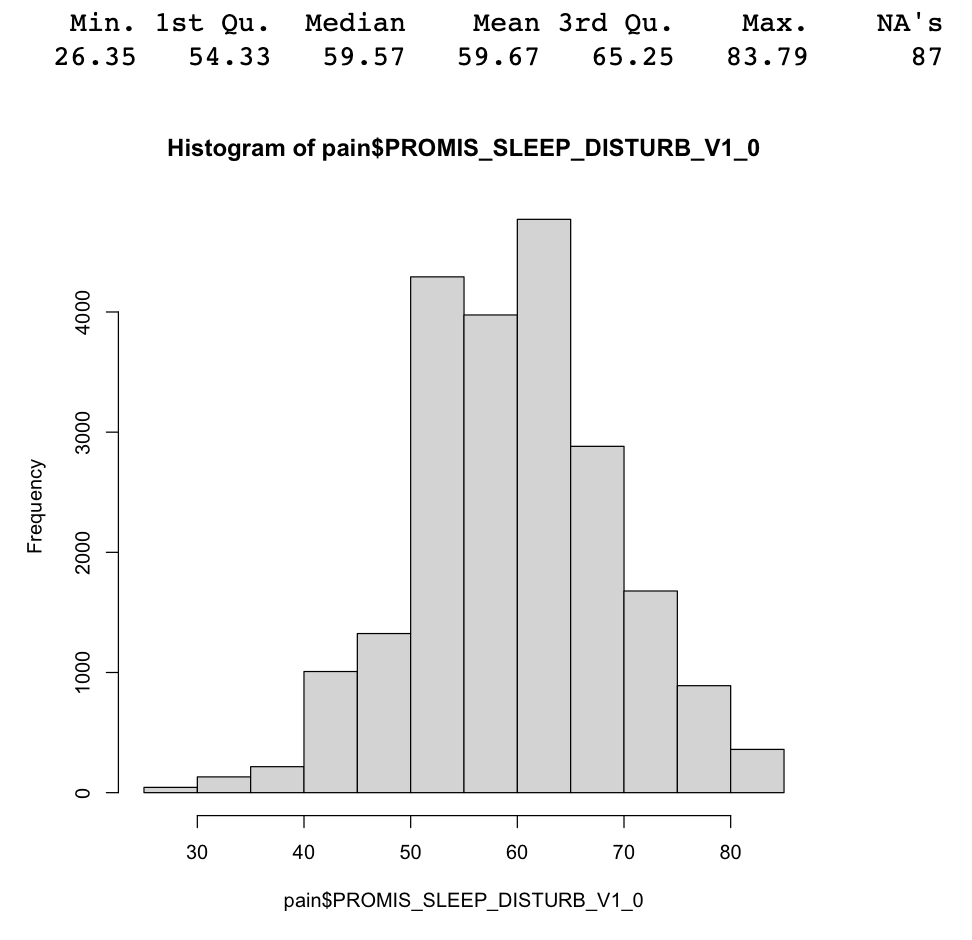
\includegraphics[width=4.16667in,height=\textheight]{book/images/3-practicequestion1answer.png}

}

\caption{\label{fig-pq1}Summarizing a Column.}

\end{figure}

\begin{Shaded}
\begin{Highlighting}[]
\CommentTok{\# Insert your solution here:}
\end{Highlighting}
\end{Shaded}

We can also use the \texttt{summary()} function for categorical
variables. In this case, R will find the counts for each level.

\begin{Shaded}
\begin{Highlighting}[]
\FunctionTok{summary}\NormalTok{(pain}\SpecialCharTok{$}\NormalTok{PAT\_SEX)}
\CommentTok{\#\textgreater{}    Length     Class      Mode }
\CommentTok{\#\textgreater{}     21659 character character}
\end{Highlighting}
\end{Shaded}

For categorical columns, it is also useful to use the \texttt{table()}
function, which returns the counts for each possible value, instead of
the \texttt{summary()} function. By default, \texttt{table()} ignores NA
values. However, we can set \texttt{useNA="always"} if we also want to
display the number of NA values in the table output. Additionally, we
can use the \texttt{prop.table()} function to convert the counts to
proportions. Below, we can see that the column \texttt{PAT\_SEX} column,
which corresponds to the reported patient sex, has a single missing
value, and we can also see that around 60\% of patients are female.

\begin{Shaded}
\begin{Highlighting}[]
\FunctionTok{table}\NormalTok{(pain}\SpecialCharTok{$}\NormalTok{PAT\_SEX, }\AttributeTok{useNA=}\StringTok{"always"}\NormalTok{)}
\CommentTok{\#\textgreater{} }
\CommentTok{\#\textgreater{} female   male   \textless{}NA\textgreater{} }
\CommentTok{\#\textgreater{}  13102   8556      1}
\end{Highlighting}
\end{Shaded}

\begin{Shaded}
\begin{Highlighting}[]
\FunctionTok{prop.table}\NormalTok{(}\FunctionTok{table}\NormalTok{(pain}\SpecialCharTok{$}\NormalTok{PAT\_SEX))}
\CommentTok{\#\textgreater{} }
\CommentTok{\#\textgreater{} female   male }
\CommentTok{\#\textgreater{}  0.605  0.395}
\end{Highlighting}
\end{Shaded}

Note that this column is not actually a factor column yet, which we can
check using the \texttt{is.factor()} function. We can convert it to one
using \texttt{as.factor()}.

\begin{Shaded}
\begin{Highlighting}[]
\FunctionTok{is.factor}\NormalTok{(pain}\SpecialCharTok{$}\NormalTok{PAT\_SEX)}
\CommentTok{\#\textgreater{} [1] FALSE}
\end{Highlighting}
\end{Shaded}

\begin{Shaded}
\begin{Highlighting}[]
\NormalTok{pain}\SpecialCharTok{$}\NormalTok{PAT\_SEX }\OtherTok{\textless{}{-}} \FunctionTok{as.factor}\NormalTok{(pain}\SpecialCharTok{$}\NormalTok{PAT\_SEX)}
\FunctionTok{is.factor}\NormalTok{(pain}\SpecialCharTok{$}\NormalTok{PAT\_SEX)}
\CommentTok{\#\textgreater{} [1] TRUE}
\end{Highlighting}
\end{Shaded}

\hypertarget{other-summary-functions}{%
\subsection{Other Summary Functions}\label{other-summary-functions}}

Sometimes we want to summarize information across multiple columns or
rows. We can use the \texttt{rowSums()} and \texttt{colSums()} functions
to sum over the rows or columns of a matrix or data frame. We first
subset the data to the body pain map regions. In the first line of code,
I select the column names pertaining to these columns. This allows me to
select those columns in the second line of code and store this subset of
the data as a new data frame called \texttt{pain\_body\_map}.

\begin{Shaded}
\begin{Highlighting}[]
\NormalTok{body\_map\_cols }\OtherTok{\textless{}{-}} \FunctionTok{names}\NormalTok{(pain)[}\DecValTok{2}\SpecialCharTok{:}\DecValTok{75}\NormalTok{]}
\NormalTok{pain\_body\_map }\OtherTok{\textless{}{-}}\NormalTok{ pain[, body\_map\_cols]}
\FunctionTok{head}\NormalTok{(pain\_body\_map)}
\CommentTok{\#\textgreater{} \# A tibble: 6 x 74}
\CommentTok{\#\textgreater{}    X101  X102  X103  X104  X105  X106  X107  X108  X109  X110  X111  X112  X113}
\CommentTok{\#\textgreater{}   \textless{}dbl\textgreater{} \textless{}dbl\textgreater{} \textless{}dbl\textgreater{} \textless{}dbl\textgreater{} \textless{}dbl\textgreater{} \textless{}dbl\textgreater{} \textless{}dbl\textgreater{} \textless{}dbl\textgreater{} \textless{}dbl\textgreater{} \textless{}dbl\textgreater{} \textless{}dbl\textgreater{} \textless{}dbl\textgreater{} \textless{}dbl\textgreater{}}
\CommentTok{\#\textgreater{} 1     0     0     0     0     0     0     0     0     0     0     0     0     0}
\CommentTok{\#\textgreater{} 2     0     0     0     0     0     0     0     0     0     0     0     0     0}
\CommentTok{\#\textgreater{} 3     0     0     0     0     0     0     0     0     0     0     0     0     0}
\CommentTok{\#\textgreater{} 4     0     0     0     0     0     0     0     0     0     0     0     0     0}
\CommentTok{\#\textgreater{} 5     0     0     0     0     0     0     0     0     0     0     0     0     0}
\CommentTok{\#\textgreater{} \# i 1 more row}
\CommentTok{\#\textgreater{} \# i 61 more variables: X114 \textless{}dbl\textgreater{}, X115 \textless{}dbl\textgreater{}, X116 \textless{}dbl\textgreater{}, X117 \textless{}dbl\textgreater{},}
\CommentTok{\#\textgreater{} \#   X118 \textless{}dbl\textgreater{}, X119 \textless{}dbl\textgreater{}, X120 \textless{}dbl\textgreater{}, X121 \textless{}dbl\textgreater{}, X122 \textless{}dbl\textgreater{}, X123 \textless{}dbl\textgreater{},}
\CommentTok{\#\textgreater{} \#   X124 \textless{}dbl\textgreater{}, X125 \textless{}dbl\textgreater{}, X126 \textless{}dbl\textgreater{}, X127 \textless{}dbl\textgreater{}, X128 \textless{}dbl\textgreater{}, X129 \textless{}dbl\textgreater{},}
\CommentTok{\#\textgreater{} \#   X130 \textless{}dbl\textgreater{}, X131 \textless{}dbl\textgreater{}, X132 \textless{}dbl\textgreater{}, X133 \textless{}dbl\textgreater{}, X134 \textless{}dbl\textgreater{}, X135 \textless{}dbl\textgreater{},}
\CommentTok{\#\textgreater{} \#   X136 \textless{}dbl\textgreater{}, X201 \textless{}dbl\textgreater{}, X202 \textless{}dbl\textgreater{}, X203 \textless{}dbl\textgreater{}, X204 \textless{}dbl\textgreater{}, X205 \textless{}dbl\textgreater{},}
\CommentTok{\#\textgreater{} \#   X206 \textless{}dbl\textgreater{}, X207 \textless{}dbl\textgreater{}, X208 \textless{}dbl\textgreater{}, X209 \textless{}dbl\textgreater{}, X210 \textless{}dbl\textgreater{}, X211 \textless{}dbl\textgreater{}, ...}
\end{Highlighting}
\end{Shaded}

I now compute the row sums and column sums on this subset of data. The
row sum for each patient is the total number of body parts in which they
experience pain, whereas the column sum for each pain region is the
total number of patients who experience pain in that area. The histogram
below shows that most people select a low number of total regions.

\begin{Shaded}
\begin{Highlighting}[]
\FunctionTok{hist}\NormalTok{(}\FunctionTok{rowSums}\NormalTok{(pain\_body\_map))}
\end{Highlighting}
\end{Shaded}

\begin{figure}[H]

{\centering 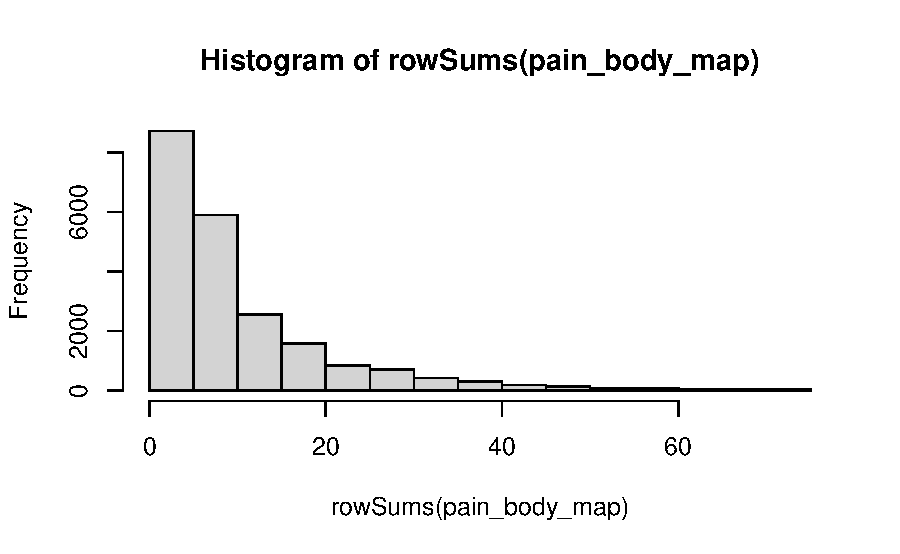
\includegraphics[width=1\textwidth,height=\textheight]{book/3_data_files_files/figure-pdf/unnamed-chunk-20-1.pdf}

}

\end{figure}

We can also see that some body parts are more often selected than
others. We create a vector called \texttt{perc\_patients} below by
finding the number of patients who selected each region divided by the
total number of patients. The histogram shows that some body regions are
selected by over 50\% of patients!

\begin{Shaded}
\begin{Highlighting}[]
\NormalTok{perc\_patients }\OtherTok{\textless{}{-}} \FunctionTok{colSums}\NormalTok{(pain\_body\_map, }\AttributeTok{na.rm=}\ConstantTok{TRUE}\NormalTok{)}\SpecialCharTok{/}\FunctionTok{nrow}\NormalTok{(pain\_body\_map)}
\FunctionTok{hist}\NormalTok{(perc\_patients)}
\end{Highlighting}
\end{Shaded}

\begin{figure}[H]

{\centering 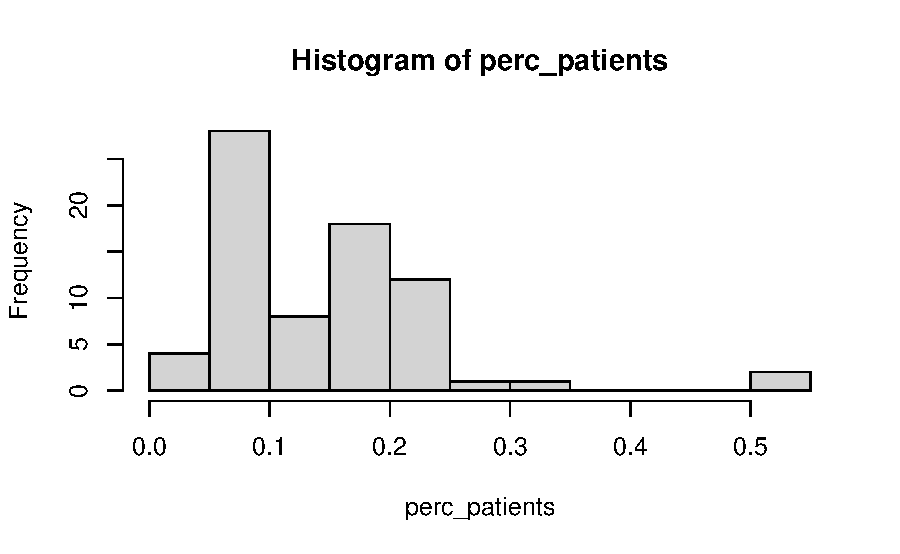
\includegraphics[width=1\textwidth,height=\textheight]{book/3_data_files_files/figure-pdf/unnamed-chunk-21-1.pdf}

}

\end{figure}

We use the \texttt{which.max()} function to see that the 55th region
\texttt{X219} is selected the most number of times. This corresponds to
lower back pain.

\begin{Shaded}
\begin{Highlighting}[]
\FunctionTok{which.max}\NormalTok{(perc\_patients)}
\CommentTok{\#\textgreater{} X219 }
\CommentTok{\#\textgreater{}   55}
\end{Highlighting}
\end{Shaded}

Another pair of useful functions are \texttt{pmin()} and
\texttt{pmax()}. These functions take at least two vectors and find the
pairwise minimum of maximum across those vectors, as shown below. For
example, suppose you had two vectors,

\begin{Shaded}
\begin{Highlighting}[]
\NormalTok{v1 }\OtherTok{=} \FunctionTok{c}\NormalTok{(}\DecValTok{5}\NormalTok{, }\DecValTok{9}\NormalTok{, }\DecValTok{12}\NormalTok{)}
\NormalTok{v2 }\OtherTok{=} \FunctionTok{c}\NormalTok{(}\DecValTok{2}\NormalTok{, }\DecValTok{18}\NormalTok{, }\DecValTok{4}\NormalTok{)}
\FunctionTok{pmax}\NormalTok{(v1, v2)  }
\CommentTok{\#\textgreater{} [1]  5 18 12}
\end{Highlighting}
\end{Shaded}

Looking back at the \texttt{pain} data, if we want to create a new
column \texttt{lower\_back\_pain} that corresponds to whether someone
selects \emph{either} X218 or X219 we can use the \texttt{pmax()}
function to find the maximum value between columns \texttt{X218} and
\texttt{X219}. We can see that almost 60\% of patients select at least
one of these regions.

\begin{Shaded}
\begin{Highlighting}[]
\NormalTok{lower\_back }\OtherTok{\textless{}{-}} \FunctionTok{pmax}\NormalTok{(pain\_body\_map}\SpecialCharTok{$}\NormalTok{X218, pain\_body\_map}\SpecialCharTok{$}\NormalTok{X219)}
\FunctionTok{prop.table}\NormalTok{(}\FunctionTok{table}\NormalTok{(lower\_back))}
\CommentTok{\#\textgreater{} lower\_back}
\CommentTok{\#\textgreater{}     0     1 }
\CommentTok{\#\textgreater{} 0.405 0.595}
\end{Highlighting}
\end{Shaded}

We might want to store the total number of pain regions and our
indicator of whether or not a patient has lower back pain as new
columns. We use our code above to create new columns in the pain data
using the \texttt{\$} operator. To be consistent with the column naming
in the data, we use all upper case for our column names. The
\texttt{dim()} function shows that our data has grown by two columns, as
expected.

\begin{Shaded}
\begin{Highlighting}[]
\NormalTok{pain}\SpecialCharTok{$}\NormalTok{NUM\_REGIONS }\OtherTok{\textless{}{-}} \FunctionTok{rowSums}\NormalTok{(pain\_body\_map)}
\NormalTok{pain}\SpecialCharTok{$}\NormalTok{LOWER\_BACK }\OtherTok{\textless{}{-}}\NormalTok{ lower\_back}
\FunctionTok{dim}\NormalTok{(pain)}
\CommentTok{\#\textgreater{} [1] 21659    94}
\end{Highlighting}
\end{Shaded}

Another useful function that allows us to perform computations over the
rows or columns of a matrix or data frame is the
\texttt{apply(X,\ MARGIN,\ FUN)} function, which takes in three
arguments. The first argument is a data frame or matrix \texttt{X}, the
second argument \texttt{MARGIN} indicates whether to compute over the
rows (\texttt{1}) or columns (\texttt{2}), and the last argument is the
function \texttt{FUN} to apply across that margin. The first example
below finds the maximum value for each row in the data frame
\texttt{pain\_body\_map}. Taking the minimum value of the row maximum
values shows that every patient selected at least one body map region.
In the second example, we find the sum of the body pain regions over the
columns, which is equivalent to the example using \texttt{colSums()}
above. In this case, we added the \texttt{na.rm=TRUE} argument. The
\texttt{apply()} function will pass additional arguments to the function
\texttt{FUN}.

\begin{Shaded}
\begin{Highlighting}[]
\NormalTok{any\_selected }\OtherTok{\textless{}{-}} \FunctionTok{apply}\NormalTok{(pain\_body\_map, }\DecValTok{1}\NormalTok{, max)}
\FunctionTok{min}\NormalTok{(any\_selected, }\AttributeTok{na.rm=}\ConstantTok{TRUE}\NormalTok{)}
\CommentTok{\#\textgreater{} [1] 1}
\end{Highlighting}
\end{Shaded}

\begin{Shaded}
\begin{Highlighting}[]
\NormalTok{perc\_patients }\OtherTok{\textless{}{-}} \FunctionTok{apply}\NormalTok{(pain\_body\_map, }\DecValTok{2}\NormalTok{, sum, }\AttributeTok{na.rm=}\ConstantTok{TRUE}\NormalTok{)}\SpecialCharTok{/}\FunctionTok{nrow}\NormalTok{(pain\_body\_map)}
\FunctionTok{summary}\NormalTok{(perc\_patients)}
\CommentTok{\#\textgreater{}    Min. 1st Qu.  Median    Mean 3rd Qu.    Max. }
\CommentTok{\#\textgreater{}   0.032   0.070   0.136   0.144   0.181   0.542}
\end{Highlighting}
\end{Shaded}

\hypertarget{practice-question-4}{%
\subsection{Practice Question}\label{practice-question-4}}

Find the sum of each of the PROMIS measures across all patients using
\texttt{apply()} and then using \texttt{colSums()}. Verify that these
two methods return the same result, which is given in
Figure~\ref{fig-pq2}.

\begin{figure}

{\centering 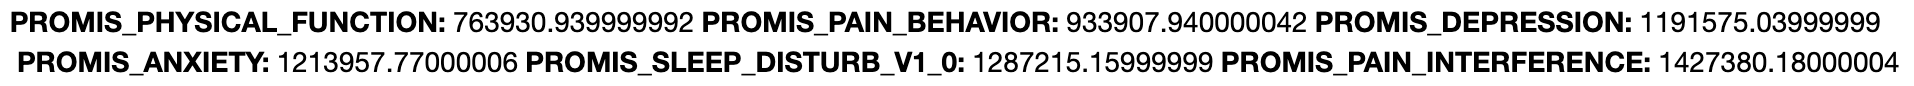
\includegraphics[width=4.16667in,height=\textheight]{book/images/3-practicequestion2answer.png}

}

\caption{\label{fig-pq2}Summing Across Columns.}

\end{figure}

\begin{Shaded}
\begin{Highlighting}[]
\CommentTok{\# Insert your solution here:}
\end{Highlighting}
\end{Shaded}

\hypertarget{missing-infinite-and-nan-values}{%
\subsection{Missing, Infinite, and NaN
Values}\label{missing-infinite-and-nan-values}}

As we saw above, this data contains some missing values, which are
represented as \texttt{NA} in R. R treats these values as if they were
unknown, which is why we have to add the \texttt{na.rm=TRUE} argument to
functions like \texttt{sum()} and \texttt{max()}. In the example below,
we can see that R figures out that 1 plus an unknown number is also
unknown!

\begin{Shaded}
\begin{Highlighting}[]
\ConstantTok{NA}\SpecialCharTok{+}\DecValTok{1}
\CommentTok{\#\textgreater{} [1] NA}
\end{Highlighting}
\end{Shaded}

We can determine whether a value is missing using the function
\texttt{is.na()}. This function returns \texttt{TRUE} if the value is NA
and \texttt{FALSE} otherwise. We can then sum up these values for a
single column, since each \texttt{TRUE} value corresponds to a value of
1 and each \texttt{FALSE} corresponds to a value of 0. Below we can see
that there is a single NA value for the column \texttt{PATIENT\_NUM},
which is the patient ID number.

\begin{Shaded}
\begin{Highlighting}[]
\FunctionTok{sum}\NormalTok{(}\FunctionTok{is.na}\NormalTok{(pain}\SpecialCharTok{$}\NormalTok{PATIENT\_NUM))}
\CommentTok{\#\textgreater{} [1] 1}
\end{Highlighting}
\end{Shaded}

If we want to calculate the sum of NA values for each column instead of
just a single column, we can use the \texttt{apply} function. Since we
want to apply this computation over the columns, the second argument has
value 2. Recall that the last argument is the function we want to call
for each column. In this case, we want to apply the combination of the
\texttt{sum()} and \texttt{is.na()} function. To do so, we have to
specify this function ourselves. This is called an \textbf{anonymous
function} since it doesn't have a name.

\begin{Shaded}
\begin{Highlighting}[]
\NormalTok{num\_missing\_col }\OtherTok{\textless{}{-}} \FunctionTok{apply}\NormalTok{(pain, }\DecValTok{2}\NormalTok{, }\ControlFlowTok{function}\NormalTok{(x) }\FunctionTok{sum}\NormalTok{(}\FunctionTok{is.na}\NormalTok{(x)))}
\FunctionTok{min}\NormalTok{(num\_missing\_col)}
\CommentTok{\#\textgreater{} [1] 1}
\end{Highlighting}
\end{Shaded}

Interestingly, we can see that there is at least one missing value in
each column. It might be the case that there is a row with all NA
values. Let's apply the same function by row. Taking the maximum, we can
see that row 11749 has all NA values.

\begin{Shaded}
\begin{Highlighting}[]
\NormalTok{num\_missing\_row }\OtherTok{\textless{}{-}} \FunctionTok{apply}\NormalTok{(pain, }\DecValTok{1}\NormalTok{, }\ControlFlowTok{function}\NormalTok{(x) }\FunctionTok{sum}\NormalTok{(}\FunctionTok{is.na}\NormalTok{(x)))}
\FunctionTok{max}\NormalTok{(num\_missing\_row)}
\CommentTok{\#\textgreater{} [1] 94}
\FunctionTok{which.max}\NormalTok{(num\_missing\_row)}
\CommentTok{\#\textgreater{} [1] 11749}
\end{Highlighting}
\end{Shaded}

We remove that row and then find the percentage of missing values by
column. We can see that the column with the highest percentage of
missing values is the pain intensity at follow-up. In fact, only 33\% of
patients have a recorded follow-up visit.

\begin{Shaded}
\begin{Highlighting}[]
\NormalTok{pain }\OtherTok{\textless{}{-}}\NormalTok{ pain[}\SpecialCharTok{{-}}\DecValTok{11749}\NormalTok{,]}
\NormalTok{num\_missing\_col }\OtherTok{\textless{}{-}} \FunctionTok{apply}\NormalTok{(pain, }\DecValTok{2}\NormalTok{, }\ControlFlowTok{function}\NormalTok{(x) }\FunctionTok{sum}\NormalTok{(}\FunctionTok{is.na}\NormalTok{(x))}\SpecialCharTok{/}\FunctionTok{nrow}\NormalTok{(pain))}
\NormalTok{num\_missing\_col}
\CommentTok{\#\textgreater{}                      PATIENT\_NUM                             X101 }
\CommentTok{\#\textgreater{}                          0.00000                          0.00000 }
\CommentTok{\#\textgreater{}                             X102                             X103 }
\CommentTok{\#\textgreater{}                          0.00000                          0.00000 }
\CommentTok{\#\textgreater{}                             X104                             X105 }
\CommentTok{\#\textgreater{}                          0.00000                          0.00000 }
\CommentTok{\#\textgreater{}                             X106                             X107 }
\CommentTok{\#\textgreater{}                          0.00000                          0.00000 }
\CommentTok{\#\textgreater{}                             X108                             X109 }
\CommentTok{\#\textgreater{}                          0.00000                          0.00000 }
\CommentTok{\#\textgreater{}                             X110                             X111 }
\CommentTok{\#\textgreater{}                          0.00000                          0.00000 }
\CommentTok{\#\textgreater{}                             X112                             X113 }
\CommentTok{\#\textgreater{}                          0.00000                          0.00000 }
\CommentTok{\#\textgreater{}                             X114                             X115 }
\CommentTok{\#\textgreater{}                          0.00000                          0.00000 }
\CommentTok{\#\textgreater{}                             X116                             X117 }
\CommentTok{\#\textgreater{}                          0.00000                          0.00000 }
\CommentTok{\#\textgreater{}                             X118                             X119 }
\CommentTok{\#\textgreater{}                          0.00000                          0.00000 }
\CommentTok{\#\textgreater{}                             X120                             X121 }
\CommentTok{\#\textgreater{}                          0.00000                          0.00000 }
\CommentTok{\#\textgreater{}                             X122                             X123 }
\CommentTok{\#\textgreater{}                          0.00000                          0.00000 }
\CommentTok{\#\textgreater{}                             X124                             X125 }
\CommentTok{\#\textgreater{}                          0.00000                          0.00000 }
\CommentTok{\#\textgreater{}                             X126                             X127 }
\CommentTok{\#\textgreater{}                          0.00000                          0.00000 }
\CommentTok{\#\textgreater{}                             X128                             X129 }
\CommentTok{\#\textgreater{}                          0.00000                          0.00000 }
\CommentTok{\#\textgreater{}                             X130                             X131 }
\CommentTok{\#\textgreater{}                          0.00000                          0.00000 }
\CommentTok{\#\textgreater{}                             X132                             X133 }
\CommentTok{\#\textgreater{}                          0.00000                          0.00000 }
\CommentTok{\#\textgreater{}                             X134                             X135 }
\CommentTok{\#\textgreater{}                          0.00000                          0.00000 }
\CommentTok{\#\textgreater{}                             X136                             X201 }
\CommentTok{\#\textgreater{}                          0.00000                          0.00000 }
\CommentTok{\#\textgreater{}                             X202                             X203 }
\CommentTok{\#\textgreater{}                          0.00000                          0.00000 }
\CommentTok{\#\textgreater{}                             X204                             X205 }
\CommentTok{\#\textgreater{}                          0.00000                          0.00000 }
\CommentTok{\#\textgreater{}                             X206                             X207 }
\CommentTok{\#\textgreater{}                          0.00000                          0.00000 }
\CommentTok{\#\textgreater{}                             X208                             X209 }
\CommentTok{\#\textgreater{}                          0.00000                          0.00000 }
\CommentTok{\#\textgreater{}                             X210                             X211 }
\CommentTok{\#\textgreater{}                          0.00000                          0.00000 }
\CommentTok{\#\textgreater{}                             X212                             X213 }
\CommentTok{\#\textgreater{}                          0.00000                          0.00000 }
\CommentTok{\#\textgreater{}                             X214                             X215 }
\CommentTok{\#\textgreater{}                          0.00000                          0.00000 }
\CommentTok{\#\textgreater{}                             X216                             X217 }
\CommentTok{\#\textgreater{}                          0.00000                          0.00000 }
\CommentTok{\#\textgreater{}                             X218                             X219 }
\CommentTok{\#\textgreater{}                          0.00000                          0.00000 }
\CommentTok{\#\textgreater{}                             X220                             X221 }
\CommentTok{\#\textgreater{}                          0.00000                          0.00000 }
\CommentTok{\#\textgreater{}                             X222                             X223 }
\CommentTok{\#\textgreater{}                          0.00000                          0.00000 }
\CommentTok{\#\textgreater{}                             X224                             X225 }
\CommentTok{\#\textgreater{}                          0.00000                          0.00000 }
\CommentTok{\#\textgreater{}                             X226                             X227 }
\CommentTok{\#\textgreater{}                          0.00000                          0.00000 }
\CommentTok{\#\textgreater{}                             X228                             X229 }
\CommentTok{\#\textgreater{}                          0.00000                          0.00000 }
\CommentTok{\#\textgreater{}                             X230                             X231 }
\CommentTok{\#\textgreater{}                          0.00000                          0.00000 }
\CommentTok{\#\textgreater{}                             X232                             X233 }
\CommentTok{\#\textgreater{}                          0.00000                          0.00000 }
\CommentTok{\#\textgreater{}                             X234                             X235 }
\CommentTok{\#\textgreater{}                          0.00000                          0.00000 }
\CommentTok{\#\textgreater{}                             X236                             X237 }
\CommentTok{\#\textgreater{}                          0.00000                          0.00000 }
\CommentTok{\#\textgreater{}                             X238           PAIN\_INTENSITY\_AVERAGE }
\CommentTok{\#\textgreater{}                          0.00000                          0.00000 }
\CommentTok{\#\textgreater{}         PROMIS\_PHYSICAL\_FUNCTION             PROMIS\_PAIN\_BEHAVIOR }
\CommentTok{\#\textgreater{}                          0.00000                          0.29412 }
\CommentTok{\#\textgreater{}                PROMIS\_DEPRESSION                   PROMIS\_ANXIETY }
\CommentTok{\#\textgreater{}                          0.00402                          0.00402 }
\CommentTok{\#\textgreater{}        PROMIS\_SLEEP\_DISTURB\_V1\_0         PROMIS\_PAIN\_INTERFERENCE }
\CommentTok{\#\textgreater{}                          0.00402                          0.00697 }
\CommentTok{\#\textgreater{}                  GH\_MENTAL\_SCORE                GH\_PHYSICAL\_SCORE }
\CommentTok{\#\textgreater{}                          0.13602                          0.13602 }
\CommentTok{\#\textgreater{}                   AGE\_AT\_CONTACT                              BMI }
\CommentTok{\#\textgreater{}                          0.00000                          0.26004 }
\CommentTok{\#\textgreater{}                  CCI\_TOTAL\_SCORE PAIN\_INTENSITY\_AVERAGE.FOLLOW\_UP }
\CommentTok{\#\textgreater{}                          0.00000                          0.67042 }
\CommentTok{\#\textgreater{}                          PAT\_SEX                         PAT\_RACE }
\CommentTok{\#\textgreater{}                          0.00000                          0.00651 }
\CommentTok{\#\textgreater{}                          CCI\_BIN                     MEDICAID\_BIN }
\CommentTok{\#\textgreater{}                          0.00000                          0.01385 }
\CommentTok{\#\textgreater{}                      NUM\_REGIONS                       LOWER\_BACK }
\CommentTok{\#\textgreater{}                          0.00000                          0.00000}
\end{Highlighting}
\end{Shaded}

We will create two new columns: first, we create a column for the change
in pain at follow-up, and second, we create a column which is the
percent change in pain at follow-up.

\begin{Shaded}
\begin{Highlighting}[]
\NormalTok{pain}\SpecialCharTok{$}\NormalTok{PAIN\_CHANGE }\OtherTok{\textless{}{-}}\NormalTok{ pain}\SpecialCharTok{$}\NormalTok{PAIN\_INTENSITY\_AVERAGE.FOLLOW\_UP }\SpecialCharTok{{-}} 
\NormalTok{  pain}\SpecialCharTok{$}\NormalTok{PAIN\_INTENSITY\_AVERAGE}
\FunctionTok{hist}\NormalTok{(pain}\SpecialCharTok{$}\NormalTok{PAIN\_CHANGE)}
\end{Highlighting}
\end{Shaded}

\begin{figure}[H]

{\centering 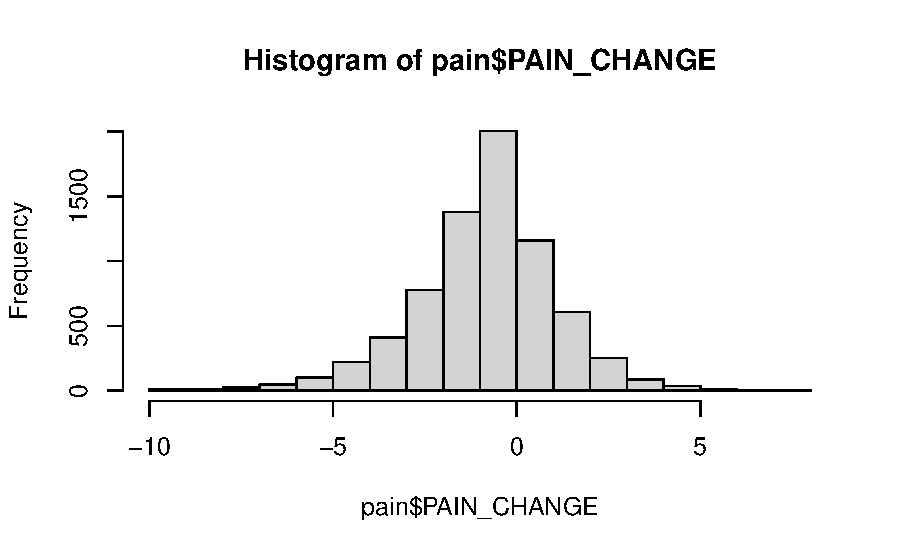
\includegraphics[width=1\textwidth,height=\textheight]{book/3_data_files_files/figure-pdf/unnamed-chunk-34-1.pdf}

}

\end{figure}

\begin{Shaded}
\begin{Highlighting}[]
\NormalTok{pain}\SpecialCharTok{$}\NormalTok{PERC\_PAIN\_CHANGE }\OtherTok{\textless{}{-}}\NormalTok{ pain}\SpecialCharTok{$}\NormalTok{PAIN\_CHANGE}\SpecialCharTok{/}\NormalTok{pain}\SpecialCharTok{$}\NormalTok{PAIN\_INTENSITY\_AVERAGE}
\FunctionTok{summary}\NormalTok{(pain}\SpecialCharTok{$}\NormalTok{PERC\_PAIN\_CHANGE)}
\CommentTok{\#\textgreater{}    Min. 1st Qu.  Median    Mean 3rd Qu.    Max.    NA\textquotesingle{}s }
\CommentTok{\#\textgreater{}      {-}1       0       0     Inf       0     Inf   14520}
\end{Highlighting}
\end{Shaded}

In the summary of the percent change, we can see that the maximum value
is \texttt{Inf}. This is R's representation of infinity. This occurred
because some patients have an initial pain score of 0, which creates
infinite values when we divide through by this value to find the percent
change. We can test whether something is infinite using the
\texttt{is.infinite()} or \texttt{is.finite()} functions. This shows
that there were three patients with infinite values. The value
\texttt{-Inf} is used to represent negative infinity.

\begin{Shaded}
\begin{Highlighting}[]
\FunctionTok{sum}\NormalTok{(}\FunctionTok{is.infinite}\NormalTok{(pain}\SpecialCharTok{$}\NormalTok{PERC\_PAIN\_CHANGE))}
\CommentTok{\#\textgreater{} [1] 3}
\end{Highlighting}
\end{Shaded}

Another special value in R is \texttt{NaN}, which stands for ``Not a
Number''. For example, \texttt{0/0} will result in a NaN value. We can
test for \texttt{NaN} values using the \texttt{is.nan()} function.

\begin{Shaded}
\begin{Highlighting}[]
\DecValTok{0}\SpecialCharTok{/}\DecValTok{0}
\CommentTok{\#\textgreater{} [1] NaN}
\end{Highlighting}
\end{Shaded}

Looking back at the missing values, there are two useful functions for
selecting the complete cases in a data frame. The \texttt{na.omit()}
function returns the data frame with incomplete cases removed, whereas
\texttt{complete.cases()} returns TRUE/FALSE values for each row
indicating whether each row is complete, which we can then use to select
the rows with TRUE values. Below, we see both approaches select the same
number of rows.

\begin{Shaded}
\begin{Highlighting}[]
\NormalTok{pain\_sub1 }\OtherTok{\textless{}{-}} \FunctionTok{na.omit}\NormalTok{(pain)}
\NormalTok{pain\_sub2 }\OtherTok{\textless{}{-}}\NormalTok{ pain[}\FunctionTok{complete.cases}\NormalTok{(pain),]}
\FunctionTok{dim}\NormalTok{(pain\_sub1)}
\CommentTok{\#\textgreater{} [1] 2413   96}
\FunctionTok{dim}\NormalTok{(pain\_sub2)}
\CommentTok{\#\textgreater{} [1] 2413   96}
\end{Highlighting}
\end{Shaded}

\hypertarget{using-logic-to-subset-summarize-and-transform}{%
\section{Using Logic to Subset, Summarize, and
Transform}\label{using-logic-to-subset-summarize-and-transform}}

Above, we used TRUE/FALSE values to select rows in a data frame. The
logic operators in R allow us to expand on this capability to write more
complex logic. The operators are given below.

\begin{itemize}
\tightlist
\item
  \texttt{\textless{}} less than
\item
  \texttt{\textless{}=} less than or equal to
\item
  \texttt{\textgreater{}} greater than
\item
  \texttt{\textgreater{}=} greater than or equal to
\item
  \texttt{==} equal to
\item
  \texttt{!=} not equal to
\item
  \texttt{a\ \%in\%\ b} a's value is in a vector of values b
\end{itemize}

The first six operators are a direct comparison between two values and
are demonstrated below.

\begin{Shaded}
\begin{Highlighting}[]
\DecValTok{2} \SpecialCharTok{\textless{}} \DecValTok{2}
\CommentTok{\#\textgreater{} [1] FALSE}
\DecValTok{2} \SpecialCharTok{\textless{}=} \DecValTok{2}
\CommentTok{\#\textgreater{} [1] TRUE}
\DecValTok{3} \SpecialCharTok{\textgreater{}} \DecValTok{2}
\CommentTok{\#\textgreater{} [1] TRUE}
\DecValTok{3} \SpecialCharTok{\textgreater{}=} \DecValTok{2}
\CommentTok{\#\textgreater{} [1] TRUE}
\StringTok{"A"} \SpecialCharTok{==} \StringTok{"B"}
\CommentTok{\#\textgreater{} [1] FALSE}
\StringTok{"A"} \SpecialCharTok{!=} \StringTok{"B"}
\CommentTok{\#\textgreater{} [1] TRUE}
\end{Highlighting}
\end{Shaded}

The operators assume there is a natural ordering or comparison between
values. For example, for strings the ordering is alphabetical and for
logical operators we use their numeric interpretation (TRUE = 1, FALSE =
0).

\begin{Shaded}
\begin{Highlighting}[]
\StringTok{"A"} \SpecialCharTok{\textless{}} \StringTok{"B"}
\CommentTok{\#\textgreater{} [1] TRUE}
\ConstantTok{TRUE} \SpecialCharTok{\textless{}} \ConstantTok{FALSE}
\CommentTok{\#\textgreater{} [1] FALSE}
\end{Highlighting}
\end{Shaded}

The \texttt{\%in\%} operator is slightly different. This operator checks
whether a value is in a set of possible values. Below, we can check
whether values are in the set \texttt{c(4,1,2)}.

\begin{Shaded}
\begin{Highlighting}[]
\DecValTok{1} \SpecialCharTok{\%in\%} \FunctionTok{c}\NormalTok{(}\DecValTok{4}\NormalTok{,}\DecValTok{1}\NormalTok{,}\DecValTok{2}\NormalTok{)}
\CommentTok{\#\textgreater{} [1] TRUE}
\FunctionTok{c}\NormalTok{(}\DecValTok{0}\NormalTok{,}\DecValTok{1}\NormalTok{,}\DecValTok{5}\NormalTok{) }\SpecialCharTok{\%in\%} \FunctionTok{c}\NormalTok{(}\DecValTok{4}\NormalTok{,}\DecValTok{1}\NormalTok{,}\DecValTok{2}\NormalTok{)}
\CommentTok{\#\textgreater{} [1] FALSE  TRUE FALSE}
\end{Highlighting}
\end{Shaded}

Additionally, we can use the following operators, which allow us to
negate or combine logical operators.

\begin{itemize}
\tightlist
\item
  \texttt{!x} - the \textbf{NOT} operator \texttt{!} reverses TRUE/FALSE
  values
\item
  \texttt{x\ \textbar{}\ y} - the \textbf{OR} operator
  \texttt{\textbar{}} checks whether \emph{either} x or y is equal to
  TRUE
\item
  \texttt{x\ \&\ y} - the \textbf{AND} operator \texttt{\&} checks
  whether \emph{both} x and y are equal to TRUE
\item
  \texttt{xor(x,y)} - the \textbf{xor} function checks whether exactly
  one of x or y is equal to TRUE (called exclusive or)
\item
  \texttt{any(x)} - the \textbf{any} function checks whether any value
  in x is TRUE (equivalent to using an OR operator \texttt{\textbar{}}
  between all values)
\item
  \texttt{all(x)} - the \textbf{all} function checks whether all values
  in x are TRUE (equivalent to using an AND operator \texttt{\&} between
  all values)
\end{itemize}

Some simple examples for each are given below.

\begin{Shaded}
\begin{Highlighting}[]
\SpecialCharTok{!}\NormalTok{(}\DecValTok{2} \SpecialCharTok{\textless{}} \DecValTok{3}\NormalTok{)}
\CommentTok{\#\textgreater{} [1] FALSE}
\NormalTok{(}\StringTok{"Alice"} \SpecialCharTok{\textless{}} \StringTok{"Bob"}\NormalTok{) }\SpecialCharTok{|}\NormalTok{ (}\StringTok{"Alice"} \SpecialCharTok{\textless{}} \StringTok{"Aaron"}\NormalTok{)}
\CommentTok{\#\textgreater{} [1] TRUE}
\NormalTok{(}\StringTok{"Alice"} \SpecialCharTok{\textless{}} \StringTok{"Bob"}\NormalTok{) }\SpecialCharTok{\&}\NormalTok{ (}\StringTok{"Alice"} \SpecialCharTok{\textless{}} \StringTok{"Aaron"}\NormalTok{)}
\CommentTok{\#\textgreater{} [1] FALSE}
\FunctionTok{xor}\NormalTok{(}\ConstantTok{TRUE}\NormalTok{, }\ConstantTok{FALSE}\NormalTok{)}
\CommentTok{\#\textgreater{} [1] TRUE}
\FunctionTok{any}\NormalTok{(}\FunctionTok{c}\NormalTok{(}\ConstantTok{FALSE}\NormalTok{, }\ConstantTok{TRUE}\NormalTok{, }\ConstantTok{TRUE}\NormalTok{))}
\CommentTok{\#\textgreater{} [1] TRUE}
\FunctionTok{all}\NormalTok{(}\FunctionTok{c}\NormalTok{(}\ConstantTok{FALSE}\NormalTok{, }\ConstantTok{TRUE}\NormalTok{, }\ConstantTok{TRUE}\NormalTok{))}
\CommentTok{\#\textgreater{} [1] FALSE}
\end{Highlighting}
\end{Shaded}

Let's demonstrate these operators on the pain data. We first update the
Medicaid column by making the character values more informative. The
logic on the left hand side selects those that do or do not have
Medicaid and then assigns those values to the new ones.

\begin{Shaded}
\begin{Highlighting}[]
\NormalTok{pain}\SpecialCharTok{$}\NormalTok{MEDICAID\_BIN[pain}\SpecialCharTok{$}\NormalTok{MEDICAID\_BIN }\SpecialCharTok{==} \StringTok{"no"}\NormalTok{] }\OtherTok{\textless{}{-}} \StringTok{"No Medicaid"}
\NormalTok{pain}\SpecialCharTok{$}\NormalTok{MEDICAID\_BIN[pain}\SpecialCharTok{$}\NormalTok{MEDICAID\_BIN }\SpecialCharTok{==} \StringTok{"yes"}\NormalTok{] }\OtherTok{\textless{}{-}} \StringTok{"Medicaid"}
\FunctionTok{table}\NormalTok{(pain}\SpecialCharTok{$}\NormalTok{MEDICAID\_BIN)}
\CommentTok{\#\textgreater{} }
\CommentTok{\#\textgreater{}    Medicaid No Medicaid }
\CommentTok{\#\textgreater{}        4601       16757}
\end{Highlighting}
\end{Shaded}

Additionally, we could subset the data to only those who have follow-up.
The not operator \texttt{!} will reverse the TRUE/FALSE values returned
from the \texttt{is.na()} function. Therefore, the new value will be
TRUE if the follow-up value is \emph{not} NA.

\begin{Shaded}
\begin{Highlighting}[]
\NormalTok{pain\_follow\_up }\OtherTok{\textless{}{-}}\NormalTok{ pain[}\SpecialCharTok{!}\FunctionTok{is.na}\NormalTok{(pain}\SpecialCharTok{$}\NormalTok{PAIN\_INTENSITY\_AVERAGE.FOLLOW\_UP),]}
\end{Highlighting}
\end{Shaded}

Earlier, we created a column indicating whether or not a patient has
lower back pain. We now use the \texttt{any()} function to check whether
a patient has general back pain. If at least one of these values is
equal to 1, then the function will return TRUE. If we had used the
\texttt{all()} function instead, this would check whether all values are
equal to 1, indicating that a patient has pain on their whole back.

\begin{Shaded}
\begin{Highlighting}[]
\NormalTok{pain}\SpecialCharTok{$}\NormalTok{BACK }\OtherTok{\textless{}{-}} \FunctionTok{any}\NormalTok{(pain}\SpecialCharTok{$}\NormalTok{X208}\SpecialCharTok{==}\DecValTok{1}\NormalTok{, pain}\SpecialCharTok{$}\NormalTok{X209}\SpecialCharTok{==}\DecValTok{1}\NormalTok{, pain}\SpecialCharTok{$}\NormalTok{X212}\SpecialCharTok{==}\DecValTok{1}\NormalTok{, pain}\SpecialCharTok{$}\NormalTok{X213}\SpecialCharTok{==}\DecValTok{1}\NormalTok{, }
\NormalTok{                 pain}\SpecialCharTok{$}\NormalTok{X218}\SpecialCharTok{==}\DecValTok{1}\NormalTok{, pain}\SpecialCharTok{$}\NormalTok{X219}\SpecialCharTok{==}\DecValTok{1}\NormalTok{)}
\end{Highlighting}
\end{Shaded}

\hypertarget{practice-question-5}{%
\subsection{Practice Question}\label{practice-question-5}}

Subset the \texttt{pain} data to those who have follow-up and have an
initial average pain intensity of 5 or above. Name this subset of the
data \texttt{pain\_subset}. Print the head of this data. The first 6
patient IDs in this new dataset should be 13118, 21384, 1827, 11309,
11093, and 14667.

\begin{Shaded}
\begin{Highlighting}[]
\CommentTok{\# Insert your solution here:}
\end{Highlighting}
\end{Shaded}

Lastly, we look at the column for patient race \texttt{PAT\_RACE}. The
\texttt{table()} function shows that most patients are \texttt{WHITE} or
\texttt{BLACK}. Given how few observations are in the other categories,
we may want to combine some of these levels into one.

\begin{Shaded}
\begin{Highlighting}[]
\FunctionTok{table}\NormalTok{(pain}\SpecialCharTok{$}\NormalTok{PAT\_RACE)}
\CommentTok{\#\textgreater{} }
\CommentTok{\#\textgreater{}          ALASKA NATIVE        AMERICAN INDIAN                  BLACK }
\CommentTok{\#\textgreater{}                      2                     58                   3229 }
\CommentTok{\#\textgreater{}                CHINESE               DECLINED               FILIPINO }
\CommentTok{\#\textgreater{}                     21                    121                      6 }
\CommentTok{\#\textgreater{}          GUAM/CHAMORRO               HAWAIIAN         INDIAN (ASIAN) }
\CommentTok{\#\textgreater{}                      1                      1                     49 }
\CommentTok{\#\textgreater{}               JAPANESE                 KOREAN          NOT SPECIFIED }
\CommentTok{\#\textgreater{}                      9                     10                      4 }
\CommentTok{\#\textgreater{}                  OTHER            OTHER ASIAN OTHER PACIFIC ISLANDER }
\CommentTok{\#\textgreater{}                      1                     47                     12 }
\CommentTok{\#\textgreater{}             VIETNAMESE                  WHITE }
\CommentTok{\#\textgreater{}                      6                  17940}
\end{Highlighting}
\end{Shaded}

Another way we could have found all possible values for this column is
to use the \texttt{unique()} function. This function takes in a data
frame or vector \texttt{x} and returns \texttt{x} with all duplicate
rows or values removed.

\begin{Shaded}
\begin{Highlighting}[]
\FunctionTok{unique}\NormalTok{(pain}\SpecialCharTok{$}\NormalTok{PAT\_RACE)}
\CommentTok{\#\textgreater{}  [1] "WHITE"                  "BLACK"                  "DECLINED"              }
\CommentTok{\#\textgreater{}  [4] "AMERICAN INDIAN"        "INDIAN (ASIAN)"         "ALASKA NATIVE"         }
\CommentTok{\#\textgreater{}  [7] NA                       "FILIPINO"               "JAPANESE"              }
\CommentTok{\#\textgreater{} [10] "VIETNAMESE"             "KOREAN"                 "CHINESE"               }
\CommentTok{\#\textgreater{} [13] "OTHER ASIAN"            "NOT SPECIFIED"          "HAWAIIAN"              }
\CommentTok{\#\textgreater{} [16] "OTHER PACIFIC ISLANDER" "OTHER"                  "GUAM/CHAMORRO"}
\end{Highlighting}
\end{Shaded}

To combine some of these levels, we can use the \texttt{\%in\%}
operator. We first create an Asian, Asian American, or Pacific Islander
race category and then create an American Indian or Alaska Native
category.

\begin{Shaded}
\begin{Highlighting}[]
\NormalTok{aapi\_values }\OtherTok{\textless{}{-}} \FunctionTok{c}\NormalTok{(}\StringTok{"CHINESE"}\NormalTok{, }\StringTok{"HAWAIIAN"}\NormalTok{, }\StringTok{"INDIAN (ASIAN)"}\NormalTok{, }\StringTok{"FILIPINO"}\NormalTok{, }
                 \StringTok{"VIETNAMESE"}\NormalTok{, }\StringTok{"JAPANESE"}\NormalTok{, }\StringTok{"KOREAN"}\NormalTok{, }\StringTok{"GUAM/CHAMORRO"}\NormalTok{, }
                 \StringTok{"OTHER ASIAN"}\NormalTok{, }\StringTok{"OTHER PACIFIC ISLANDER"}\NormalTok{)}
\NormalTok{pain}\SpecialCharTok{$}\NormalTok{PAT\_RACE[pain}\SpecialCharTok{$}\NormalTok{PAT\_RACE }\SpecialCharTok{\%in\%}\NormalTok{ aapi\_values] }\OtherTok{\textless{}{-}} \StringTok{"AAPI"}
\NormalTok{pain}\SpecialCharTok{$}\NormalTok{PAT\_RACE[pain}\SpecialCharTok{$}\NormalTok{PAT\_RACE }\SpecialCharTok{\%in\%} \FunctionTok{c}\NormalTok{(}\StringTok{"ALASKA NATIVE"}\NormalTok{, }\StringTok{"AMERICAN INDIAN"}\NormalTok{)] }\OtherTok{\textless{}{-}} 
  \StringTok{"AI/AN"}
\FunctionTok{table}\NormalTok{(pain}\SpecialCharTok{$}\NormalTok{PAT\_RACE)}
\CommentTok{\#\textgreater{} }
\CommentTok{\#\textgreater{}          AAPI         AI/AN         BLACK      DECLINED NOT SPECIFIED }
\CommentTok{\#\textgreater{}           162            60          3229           121             4 }
\CommentTok{\#\textgreater{}         OTHER         WHITE }
\CommentTok{\#\textgreater{}             1         17940}
\end{Highlighting}
\end{Shaded}

\hypertarget{other-selection-functions}{%
\subsection{Other Selection Functions}\label{other-selection-functions}}

Above, we selected rows using TRUE/FALSE boolean values. Instead, we
could have also used the \texttt{which()} function. This function takes
TRUE/FALSE values and returns the index values for all the TRUE values.
We use this to treat those with race given as \texttt{DECLINED} as not
specified.

\begin{Shaded}
\begin{Highlighting}[]
\NormalTok{pain}\SpecialCharTok{$}\NormalTok{PAT\_RACE[}\FunctionTok{which}\NormalTok{(pain}\SpecialCharTok{$}\NormalTok{PAT\_RACE }\SpecialCharTok{==} \StringTok{"DECLINED"}\NormalTok{)] }\OtherTok{\textless{}{-}} \StringTok{"NOT SPECIFIED"}
\end{Highlighting}
\end{Shaded}

Another selection function is the \texttt{subset()} function. This
function takes in two arguments. The first is the vector, matrix, or
data frame to select from and the second is a vector of TRUE/FALSE
values to use for row selection. We use this to find the observation
with race marked as \texttt{OTHER}. We then update this race to also be
marked as not specified.

\begin{Shaded}
\begin{Highlighting}[]
\FunctionTok{subset}\NormalTok{(pain, pain}\SpecialCharTok{$}\NormalTok{PAT\_RACE }\SpecialCharTok{==} \StringTok{"OTHER"}\NormalTok{)}
\CommentTok{\#\textgreater{} \# A tibble: 1 x 97}
\CommentTok{\#\textgreater{}   PATIENT\_NUM  X101  X102  X103  X104  X105  X106  X107  X108  X109  X110  X111}
\CommentTok{\#\textgreater{}         \textless{}dbl\textgreater{} \textless{}dbl\textgreater{} \textless{}dbl\textgreater{} \textless{}dbl\textgreater{} \textless{}dbl\textgreater{} \textless{}dbl\textgreater{} \textless{}dbl\textgreater{} \textless{}dbl\textgreater{} \textless{}dbl\textgreater{} \textless{}dbl\textgreater{} \textless{}dbl\textgreater{} \textless{}dbl\textgreater{}}
\CommentTok{\#\textgreater{} 1        3588     1     1     1     0     1     1     1     0     0     0     0}
\CommentTok{\#\textgreater{} \# i 85 more variables: X112 \textless{}dbl\textgreater{}, X113 \textless{}dbl\textgreater{}, X114 \textless{}dbl\textgreater{}, X115 \textless{}dbl\textgreater{},}
\CommentTok{\#\textgreater{} \#   X116 \textless{}dbl\textgreater{}, X117 \textless{}dbl\textgreater{}, X118 \textless{}dbl\textgreater{}, X119 \textless{}dbl\textgreater{}, X120 \textless{}dbl\textgreater{}, X121 \textless{}dbl\textgreater{},}
\CommentTok{\#\textgreater{} \#   X122 \textless{}dbl\textgreater{}, X123 \textless{}dbl\textgreater{}, X124 \textless{}dbl\textgreater{}, X125 \textless{}dbl\textgreater{}, X126 \textless{}dbl\textgreater{}, X127 \textless{}dbl\textgreater{},}
\CommentTok{\#\textgreater{} \#   X128 \textless{}dbl\textgreater{}, X129 \textless{}dbl\textgreater{}, X130 \textless{}dbl\textgreater{}, X131 \textless{}dbl\textgreater{}, X132 \textless{}dbl\textgreater{}, X133 \textless{}dbl\textgreater{},}
\CommentTok{\#\textgreater{} \#   X134 \textless{}dbl\textgreater{}, X135 \textless{}dbl\textgreater{}, X136 \textless{}dbl\textgreater{}, X201 \textless{}dbl\textgreater{}, X202 \textless{}dbl\textgreater{}, X203 \textless{}dbl\textgreater{},}
\CommentTok{\#\textgreater{} \#   X204 \textless{}dbl\textgreater{}, X205 \textless{}dbl\textgreater{}, X206 \textless{}dbl\textgreater{}, X207 \textless{}dbl\textgreater{}, X208 \textless{}dbl\textgreater{}, X209 \textless{}dbl\textgreater{},}
\CommentTok{\#\textgreater{} \#   X210 \textless{}dbl\textgreater{}, X211 \textless{}dbl\textgreater{}, X212 \textless{}dbl\textgreater{}, X213 \textless{}dbl\textgreater{}, X214 \textless{}dbl\textgreater{}, X215 \textless{}dbl\textgreater{}, ...}
\end{Highlighting}
\end{Shaded}

\begin{Shaded}
\begin{Highlighting}[]
\NormalTok{pain}\SpecialCharTok{$}\NormalTok{PAT\_RACE[pain}\SpecialCharTok{$}\NormalTok{PATIENT\_NUM}\SpecialCharTok{==}\DecValTok{3588}\NormalTok{] }\OtherTok{\textless{}{-}} \StringTok{"NOT SPECIFIED"}
\FunctionTok{table}\NormalTok{(pain}\SpecialCharTok{$}\NormalTok{PAT\_RACE)}
\CommentTok{\#\textgreater{} }
\CommentTok{\#\textgreater{}          AAPI         AI/AN         BLACK NOT SPECIFIED         WHITE }
\CommentTok{\#\textgreater{}           162            60          3229           126         17940}
\end{Highlighting}
\end{Shaded}

\hypertarget{exercises-1}{%
\section{Exercises}\label{exercises-1}}

For these exercises, we will again be using the \texttt{pain} data from
the \textbf{HDSinRdata} package.

\begin{enumerate}
\def\labelenumi{\arabic{enumi}.}
\item
  Print summary statistics for the \texttt{PROMIS\_PHYSICAL\_FUNTION}
  and \texttt{PROMIS\_ANXIETY} columns in this dataset. Read the data
  documentation for these two columns, which both have range 0 to 100,
  and then comment on the distributions of these columns.
\item
  Create frequency tables for the values of \texttt{PAT\_SEX} and
  \texttt{PAT\_RACE} and summarize what these tables tell you about the
  distributions of these demographic characteristics.
\item
  Create a new data frame called \texttt{pain.new} that doesn't contain
  patients with NA values for both \texttt{GH\_MENTAL\_SCORE} and
  \texttt{GH\_PHYSICAL\_SCORE}, which are the PROMIS global mental and
  physical scores, respectively.
\item
  Create a vector of the proportion of patients who reported pain in
  each of the pain regions. Then, find the minimum, median, mean,
  maximum, standard deviation, and variance of this vector.
\item
  Calculate the median and interquartile range of the distribution of
  the total number of painful \textbf{leg} regions selected for each
  patient. Then, write a few sentences explaining anything interesting
  you observe about this distribution in the context of this dataset.
\item
  Look at the distribution of average pain intensity between patients
  with only one pain region selected vs.~those with more than one region
  selected. What do you notice?
\item
  Create a histogram to plot the distribution of the
  \texttt{PAIN\_INTENSITY\_AVERAGE.FOLLOW\_UP} column. Then, create a
  table summarizing how many patients had missing values in this column.
  Finally, choose two columns to compare the distribution between those
  with and without missing follow up. What do you notice?
\end{enumerate}

\bookmarksetup{startatroot}

\hypertarget{sec-exploratory}{%
\chapter{Intro to Exploratory Data Analysis}\label{sec-exploratory}}

In the last chapter, we learned about loading data into R and practiced
selecting and summarizing columns and rows of the data. In this chapter,
we will learn how to conduct more exploratory analysis, focusing on the
univariate and bivariate sample distributions of the data. The first
half focuses on using base R to create basic plots and summaries. In the
second half, we show how to create summary plots using the
\textbf{GGally} package (Schloerke et al. 2021) and tables using the
\textbf{gt} (Iannone et al. 2023) and \textbf{gtsummary} (Sjoberg et al.
2023) packages.

\begin{Shaded}
\begin{Highlighting}[]
\FunctionTok{library}\NormalTok{(HDSinRdata)}
\FunctionTok{library}\NormalTok{(GGally) }
\FunctionTok{library}\NormalTok{(gt)}
\FunctionTok{library}\NormalTok{(gtsummary)}
\end{Highlighting}
\end{Shaded}

\hypertarget{univariate-distributions}{%
\section{Univariate Distributions}\label{univariate-distributions}}

In this chapter, we will use a sample of the National Health and
Nutrition Examination Survey (Disease Control and (CDC) 1999-2018)
containing lead, blood pressure, BMI, smoking status, alcohol use, and
demographic variables from NHANES 1999-2018. Variable selection and
feature engineering followed the analysis in Huang (2022). There are
31,625 observations in this sample. Use the help operator
\texttt{?NHANESsample} to read the column descriptions.

\begin{Shaded}
\begin{Highlighting}[]
\FunctionTok{data}\NormalTok{(NHANESsample)}
\FunctionTok{dim}\NormalTok{(NHANESsample)}
\CommentTok{\#\textgreater{} [1] 31265    21}
\FunctionTok{names}\NormalTok{(NHANESsample)}
\CommentTok{\#\textgreater{}  [1] "ID"            "AGE"           "SEX"           "RACE"         }
\CommentTok{\#\textgreater{}  [5] "EDUCATION"     "INCOME"        "SMOKE"         "YEAR"         }
\CommentTok{\#\textgreater{}  [9] "LEAD"          "BMI\_CAT"       "LEAD\_QUANTILE" "HYP"          }
\CommentTok{\#\textgreater{} [13] "ALC"           "DBP1"          "DBP2"          "DBP3"         }
\CommentTok{\#\textgreater{} [17] "DBP4"          "SBP1"          "SBP2"          "SBP3"         }
\CommentTok{\#\textgreater{} [21] "SBP4"}
\end{Highlighting}
\end{Shaded}

To start our exploration, we will look at whether there are any missing
values. We use the \texttt{complete.cases()} function to observe that
there are no complete cases. We also see that the subsequent blood
pressure measurements and alcohol use have the highest percentage of
missing values. For demonstration, we choose to only keep the first
systolic an diastolic blood pressure measurements and do a complete case
analysis using the \texttt{na.omit()} function to define our complete
data frame \texttt{nhanes\_df}.

\begin{Shaded}
\begin{Highlighting}[]
\FunctionTok{sum}\NormalTok{(}\FunctionTok{complete.cases}\NormalTok{(NHANESsample))}
\CommentTok{\#\textgreater{} [1] 0}
\FunctionTok{apply}\NormalTok{(NHANESsample, }\DecValTok{2}\NormalTok{, }\ControlFlowTok{function}\NormalTok{(x) }\FunctionTok{sum}\NormalTok{(}\FunctionTok{is.na}\NormalTok{(x)))}\SpecialCharTok{/}\FunctionTok{nrow}\NormalTok{(NHANESsample)}
\CommentTok{\#\textgreater{}            ID           AGE           SEX          RACE     EDUCATION }
\CommentTok{\#\textgreater{}      0.000000      0.000000      0.000000      0.000000      0.000672 }
\CommentTok{\#\textgreater{}        INCOME         SMOKE          YEAR          LEAD       BMI\_CAT }
\CommentTok{\#\textgreater{}      0.000000      0.000000      0.000000      0.000000      0.000000 }
\CommentTok{\#\textgreater{} LEAD\_QUANTILE           HYP           ALC          DBP1          DBP2 }
\CommentTok{\#\textgreater{}      0.000000      0.000000      0.026867      0.060035      0.063905 }
\CommentTok{\#\textgreater{}          DBP3          DBP4          SBP1          SBP2          SBP3 }
\CommentTok{\#\textgreater{}      0.070974      0.891124      0.060035      0.063905      0.070942 }
\CommentTok{\#\textgreater{}          SBP4 }
\CommentTok{\#\textgreater{}      0.891124}
\end{Highlighting}
\end{Shaded}

\begin{Shaded}
\begin{Highlighting}[]
\NormalTok{nhanes\_df }\OtherTok{\textless{}{-}} \FunctionTok{na.omit}\NormalTok{(}\FunctionTok{subset}\NormalTok{(NHANESsample, }
                            \AttributeTok{select=} \SpecialCharTok{{-}}\FunctionTok{c}\NormalTok{(SBP2, SBP3, SBP4, DBP2, DBP3, DBP4)))}
\end{Highlighting}
\end{Shaded}

In the last chapter, we introduced the \texttt{table()} and
\texttt{summary()} functions to quickly summarize categorical and
quantitative vectors. We can observe that over half of the observations
never smoked and that the most recent NHANES cycle in the data is
2017-2018.

\begin{Shaded}
\begin{Highlighting}[]
\FunctionTok{table}\NormalTok{(nhanes\_df}\SpecialCharTok{$}\NormalTok{SMOKE)}
\CommentTok{\#\textgreater{} }
\CommentTok{\#\textgreater{} NeverSmoke  QuitSmoke StillSmoke }
\CommentTok{\#\textgreater{}      13774       8019       6799}
\FunctionTok{summary}\NormalTok{(nhanes\_df}\SpecialCharTok{$}\NormalTok{YEAR)}
\CommentTok{\#\textgreater{}    Min. 1st Qu.  Median    Mean 3rd Qu.    Max. }
\CommentTok{\#\textgreater{}    1999    2003    2007    2008    2011    2017}
\end{Highlighting}
\end{Shaded}

We decide to select the most recent observations from NHANES 2017-2018
for our analysis in this chapter. We use the \texttt{subset()} function
to select these rows.

\begin{Shaded}
\begin{Highlighting}[]
\NormalTok{nhanes\_df }\OtherTok{\textless{}{-}} \FunctionTok{subset}\NormalTok{(nhanes\_df, nhanes\_df}\SpecialCharTok{$}\NormalTok{YEAR}\SpecialCharTok{==}\DecValTok{2017}\NormalTok{)}
\end{Highlighting}
\end{Shaded}

As shown above, smoking status has been coded into three categories:
``NeverSmoke'', ``QuitSmoke'', and ``StillSmoke''. We want to create a
new column to represent whether someone has ever smoked. To do so, we
use the \texttt{ifelse()} function, which allows us to create a new
vector using logic. The logic captured by this function is that we will
take one value if we meet some condition(s) and we will take a second
value otherwise. The first argument is a vector of TRUE/FALSE values
representing the conditions, the next argument is the value to use if we
meet the condition(s), and the last argument is the value to use
otherwise. We use this function to create a new vector
\texttt{EVER\_SMOKE} that is equal to ``Yes'' for those who are either
still smoking or quit smoking and equal to ``No'' otherwise.

\begin{Shaded}
\begin{Highlighting}[]
\NormalTok{nhanes\_df}\SpecialCharTok{$}\NormalTok{EVER\_SMOKE }\OtherTok{\textless{}{-}} \FunctionTok{ifelse}\NormalTok{(nhanes\_df}\SpecialCharTok{$}\NormalTok{SMOKE }\SpecialCharTok{\%in\%} \FunctionTok{c}\NormalTok{(}\StringTok{"QuitSmoke"}\NormalTok{, }
                                                      \StringTok{"StillSmoke"}\NormalTok{), }
                               \StringTok{"Yes"}\NormalTok{, }\StringTok{"No"}\NormalTok{)}
\FunctionTok{table}\NormalTok{(nhanes\_df}\SpecialCharTok{$}\NormalTok{EVER\_SMOKE)}
\CommentTok{\#\textgreater{} }
\CommentTok{\#\textgreater{}   No  Yes }
\CommentTok{\#\textgreater{} 1411 1173}
\end{Highlighting}
\end{Shaded}

The \texttt{summary()} and \texttt{table()} functions allow us to
summarize the univariate sample distributions of columns. We may also
want to plot these distributions. We saw in Chapter~\ref{sec-data-files}
that the \texttt{hist()} function creates a histogram plot. Below we use
this function to plot a histogram of the log transformation of the lead
column.

\begin{Shaded}
\begin{Highlighting}[]
\FunctionTok{hist}\NormalTok{(}\FunctionTok{log}\NormalTok{(nhanes\_df}\SpecialCharTok{$}\NormalTok{LEAD))}
\end{Highlighting}
\end{Shaded}

\begin{figure}[H]

{\centering 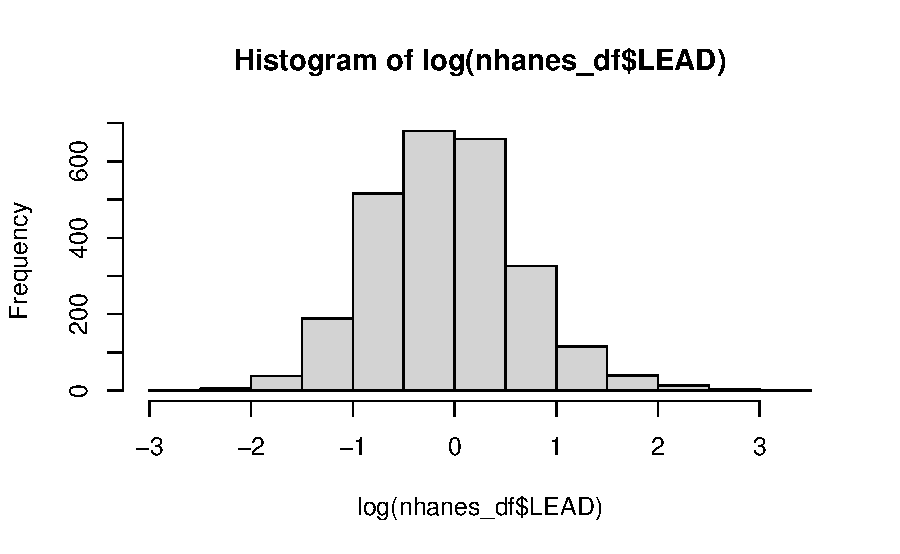
\includegraphics[width=1\textwidth,height=\textheight]{book/4_exploratory_analysis_files/figure-pdf/unnamed-chunk-8-1.pdf}

}

\end{figure}

If we want to polish this figure, we can use some of the other optional
arguments to the \texttt{hist()} function. For example, we may want to
update the text \texttt{log(nhanes\_df\$lead)} in the title and x-axis.
Below, we update the color, labels, and number of bins for the plot. The
function \texttt{colors()} returns all recognized colors in R. The
argument \texttt{breaks} specifies the number of bins to use to create
the histogram, \texttt{col} specifies the color, \texttt{main} specifies
the title of the plot, and \texttt{xlab} specifies the x-axis label
(using \texttt{ylab} would specify the y-axis label). Read the
documentation \texttt{?hist} for the full list of arguments available.

\begin{Shaded}
\begin{Highlighting}[]
\FunctionTok{hist}\NormalTok{(}\FunctionTok{log}\NormalTok{(nhanes\_df}\SpecialCharTok{$}\NormalTok{LEAD), }\AttributeTok{breaks =} \DecValTok{30}\NormalTok{, }\AttributeTok{col=}\StringTok{"blue"}\NormalTok{, }
     \AttributeTok{main=}\StringTok{"Histogram of Log Blood Lead Level"}\NormalTok{,}
     \AttributeTok{xlab=}\StringTok{"Log Blood Lead Level"}\NormalTok{)}
\end{Highlighting}
\end{Shaded}

\begin{figure}[H]

{\centering 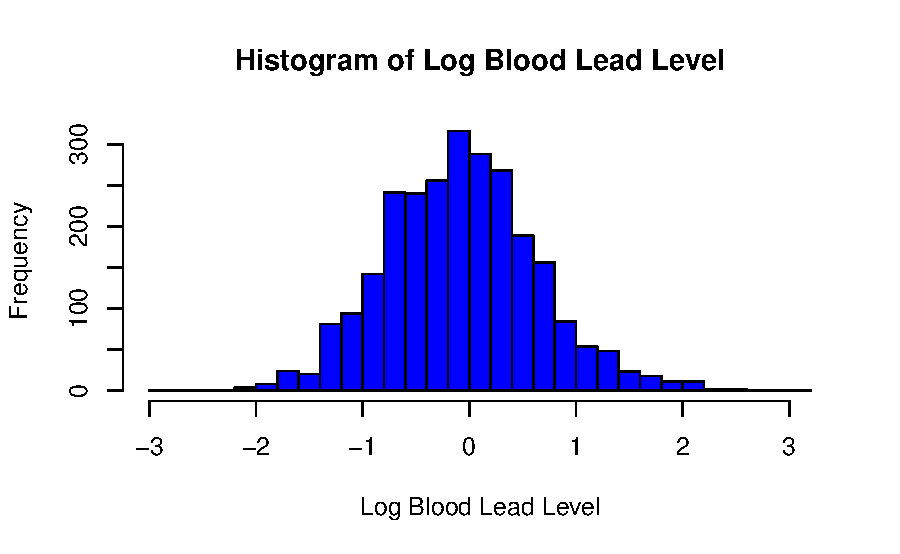
\includegraphics[width=1\textwidth,height=\textheight]{book/4_exploratory_analysis_files/figure-pdf/unnamed-chunk-9-1.pdf}

}

\end{figure}

For categorical columns, we may want to plot the counts in each category
using a bar plot. The function \texttt{barplot()} asks us to specify the
\texttt{names} and \texttt{heights} of the bars. To do so, we will need
to store the counts for each category. Again, we update the color and
labels.

\begin{Shaded}
\begin{Highlighting}[]
\NormalTok{smoke\_counts }\OtherTok{\textless{}{-}} \FunctionTok{table}\NormalTok{(nhanes\_df}\SpecialCharTok{$}\NormalTok{SMOKE)}
\FunctionTok{barplot}\NormalTok{(}\AttributeTok{height=}\NormalTok{smoke\_counts, }\AttributeTok{names=}\FunctionTok{names}\NormalTok{(smoke\_counts), }\AttributeTok{col=}\StringTok{"violetred"}\NormalTok{,}
       \AttributeTok{xlab=}\StringTok{"Smoking Status"}\NormalTok{, }\AttributeTok{ylab=}\StringTok{"Frequency"}\NormalTok{)}
\end{Highlighting}
\end{Shaded}

\begin{figure}[H]

{\centering 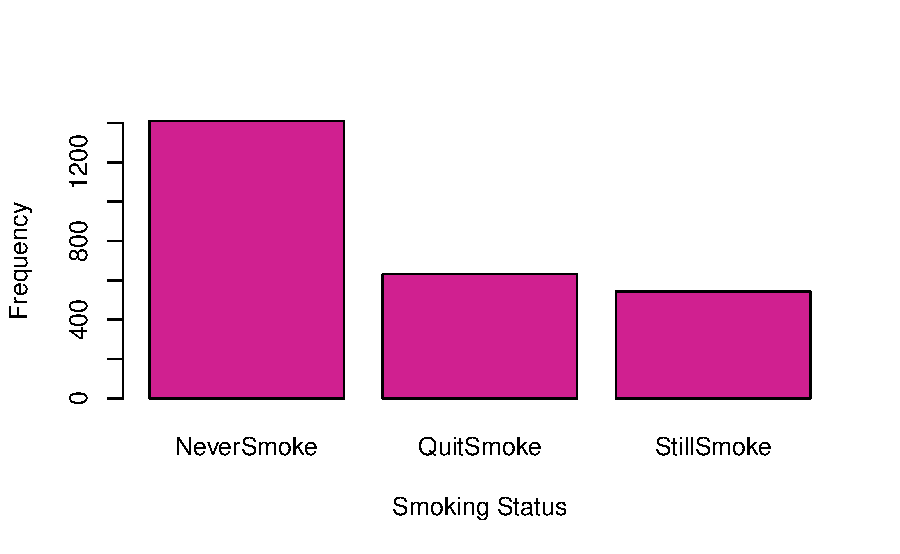
\includegraphics[width=1\textwidth,height=\textheight]{book/4_exploratory_analysis_files/figure-pdf/unnamed-chunk-10-1.pdf}

}

\end{figure}

With a bar plot, we can even specify a different color for each bar. To
do so, \texttt{col} must be a vector of specified colors with the same
length as the number of categories.

\begin{Shaded}
\begin{Highlighting}[]
\FunctionTok{barplot}\NormalTok{(}\AttributeTok{height=}\NormalTok{smoke\_counts, }\AttributeTok{names=}\FunctionTok{names}\NormalTok{(smoke\_counts), }
        \AttributeTok{col=}\FunctionTok{c}\NormalTok{(}\StringTok{"orange"}\NormalTok{,}\StringTok{"violetred"}\NormalTok{,}\StringTok{"blue"}\NormalTok{),}
        \AttributeTok{xlab=}\StringTok{"Smoking Status"}\NormalTok{, }\AttributeTok{ylab=}\StringTok{"Frequency"}\NormalTok{)}
\end{Highlighting}
\end{Shaded}

\begin{figure}[H]

{\centering 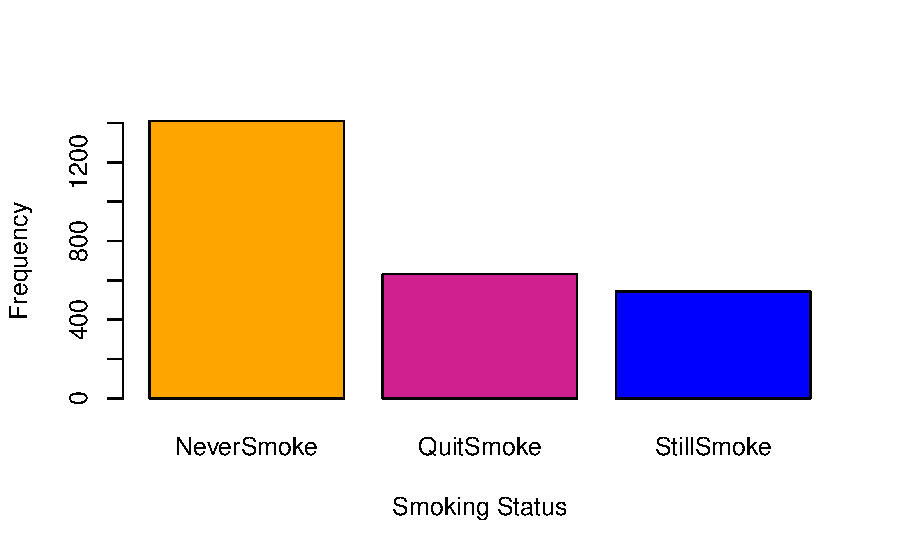
\includegraphics[width=1\textwidth,height=\textheight]{book/4_exploratory_analysis_files/figure-pdf/unnamed-chunk-11-1.pdf}

}

\end{figure}

\hypertarget{practice-question-6}{%
\subsection{Practice Question}\label{practice-question-6}}

Recreate the barplot in Figure~\ref{fig-pq1} showing the proportion of
values in each \texttt{LEAD\_QUANTILE} category.

\begin{figure}

{\centering 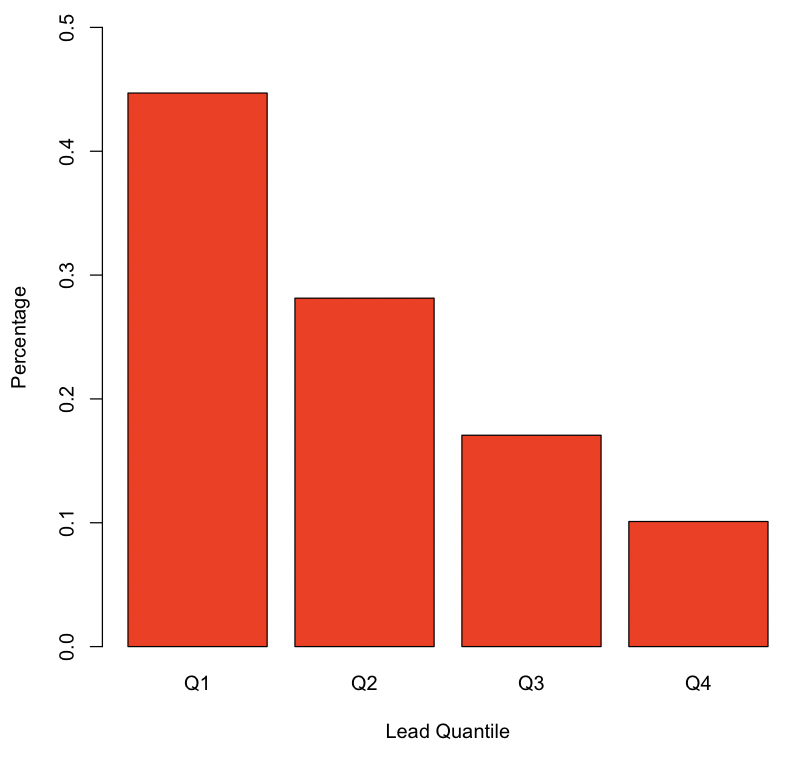
\includegraphics[width=2.77778in,height=\textheight]{book/images/4-practicequestion1answer.png}

}

\caption{\label{fig-pq1}Lead Quantile Bar Plot.}

\end{figure}

\begin{Shaded}
\begin{Highlighting}[]
\CommentTok{\# Insert your solution here:}
\end{Highlighting}
\end{Shaded}

\hypertarget{bivariate-distributions}{%
\section{Bivariate Distributions}\label{bivariate-distributions}}

We now turn our attention to relationships among multiple columns. When
we have two categorical columns, we can use the \texttt{table()}
function to find the counts across all combinations. For example, below
we look at the distribution of smoking status levels by sex. We observe
that a higher percentage of female participants have never smoked.

\begin{Shaded}
\begin{Highlighting}[]
\FunctionTok{table}\NormalTok{(nhanes\_df}\SpecialCharTok{$}\NormalTok{SMOKE, nhanes\_df}\SpecialCharTok{$}\NormalTok{SEX)}
\CommentTok{\#\textgreater{}             }
\CommentTok{\#\textgreater{}              Male Female}
\CommentTok{\#\textgreater{}   NeverSmoke  596    815}
\CommentTok{\#\textgreater{}   QuitSmoke   390    241}
\CommentTok{\#\textgreater{}   StillSmoke  324    218}
\end{Highlighting}
\end{Shaded}

To look at the sample distribution of a continuous column stratified by
a cateogrical column, we could call the \texttt{summary()} function for
each subset of the data. Below we look at the distribution of blood lead
level by sex and observe higher blood lead levels in male observations.

\begin{Shaded}
\begin{Highlighting}[]
\FunctionTok{summary}\NormalTok{(nhanes\_df}\SpecialCharTok{$}\NormalTok{LEAD[nhanes\_df}\SpecialCharTok{$}\NormalTok{SEX}\SpecialCharTok{==}\StringTok{"Female"}\NormalTok{])}
\CommentTok{\#\textgreater{}    Min. 1st Qu.  Median    Mean 3rd Qu.    Max. }
\CommentTok{\#\textgreater{}    0.10    0.47    0.77    0.98    1.21    8.67}
\FunctionTok{summary}\NormalTok{(nhanes\_df}\SpecialCharTok{$}\NormalTok{LEAD[nhanes\_df}\SpecialCharTok{$}\NormalTok{SEX}\SpecialCharTok{==}\StringTok{"Male"}\NormalTok{])}
\CommentTok{\#\textgreater{}    Min. 1st Qu.  Median    Mean 3rd Qu.    Max. }
\CommentTok{\#\textgreater{}    0.05    0.70    1.09    1.46    1.66   22.01}
\end{Highlighting}
\end{Shaded}

We could also observe this visually through a box plot. When given one
categorical column and one continuous column, the \texttt{plot()}
function creates a box plot. By default, the first argument is the
x-axis and second argument is the y-axis.

\begin{Shaded}
\begin{Highlighting}[]
\FunctionTok{plot}\NormalTok{(nhanes\_df}\SpecialCharTok{$}\NormalTok{SEX, }\FunctionTok{log}\NormalTok{(nhanes\_df}\SpecialCharTok{$}\NormalTok{LEAD), }\AttributeTok{ylab=}\StringTok{"Log Blood Lead Level"}\NormalTok{, }
     \AttributeTok{xlab=}\StringTok{"Sex"}\NormalTok{)}
\end{Highlighting}
\end{Shaded}

\begin{figure}[H]

{\centering 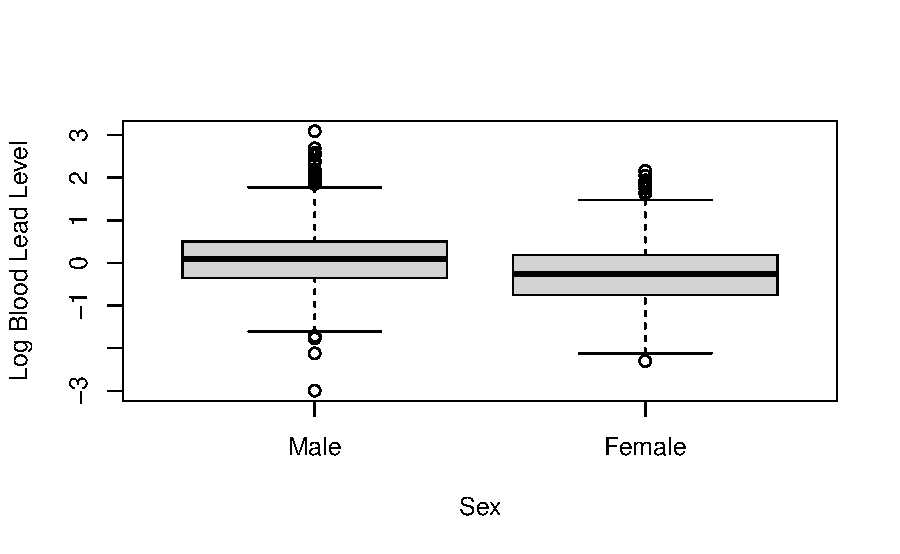
\includegraphics[width=1\textwidth,height=\textheight]{book/4_exploratory_analysis_files/figure-pdf/unnamed-chunk-15-1.pdf}

}

\end{figure}

Alternatively, we could use the \texttt{boxplot()} function, which can
be passed a formula. A formula is a string representation of how to
group the data, where the left hand side is the continuous column and
the right hand side is one or more categorical columns to group by. In
the case below, we group by multiple columns, \texttt{SEX} and
\texttt{EVER\_SMOKE}, so our formula is
\texttt{log(LEAD)\textasciitilde{}SEX+EVER\_SMOKE}. The second argument
to the function specifies the data. We specify the column colors to show
the link between the box plots shown.

\begin{Shaded}
\begin{Highlighting}[]
\FunctionTok{boxplot}\NormalTok{(}\FunctionTok{log}\NormalTok{(LEAD)}\SpecialCharTok{\textasciitilde{}}\NormalTok{SEX}\SpecialCharTok{+}\NormalTok{EVER\_SMOKE, }\AttributeTok{data=}\NormalTok{nhanes\_df, }
        \AttributeTok{col=}\FunctionTok{c}\NormalTok{(}\StringTok{"orange"}\NormalTok{, }\StringTok{"blue"}\NormalTok{, }\StringTok{"orange"}\NormalTok{, }\StringTok{"blue"}\NormalTok{),}
        \AttributeTok{xlab=}\StringTok{"Sex : Ever Smoked"}\NormalTok{, }\AttributeTok{ylab =} \StringTok{"Log Blood Lead Level"}\NormalTok{)}
\end{Highlighting}
\end{Shaded}

\begin{figure}[H]

{\centering 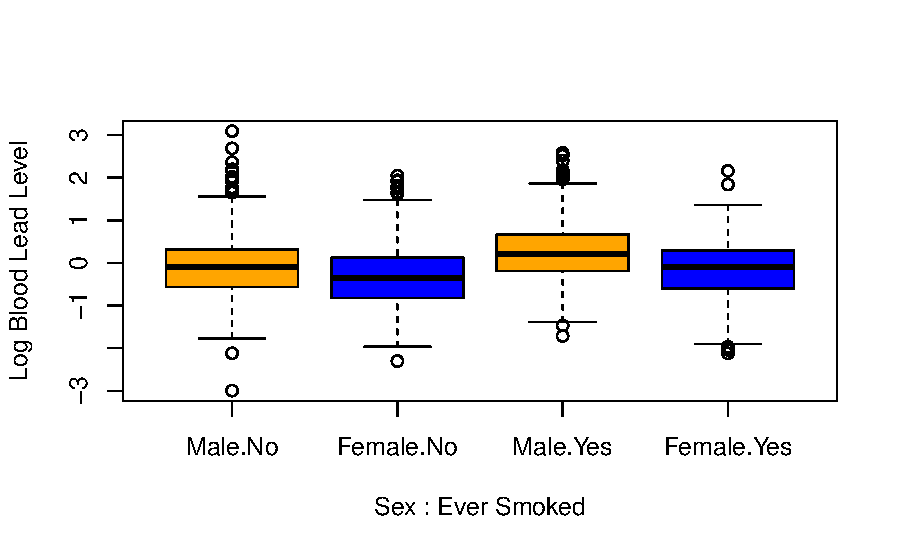
\includegraphics[width=1\textwidth,height=\textheight]{book/4_exploratory_analysis_files/figure-pdf/unnamed-chunk-16-1.pdf}

}

\end{figure}

To visualize the bivariate distributions between two continuous columns,
we can use scatter plots. To create a scatter plot, we use the
\texttt{plot()} function again. Below, we use this function to show the
relationship between systolic and diastolic blood pressure.

\begin{Shaded}
\begin{Highlighting}[]
\FunctionTok{plot}\NormalTok{(nhanes\_df}\SpecialCharTok{$}\NormalTok{SBP1, nhanes\_df}\SpecialCharTok{$}\NormalTok{DBP1, }\AttributeTok{col=}\StringTok{"blue"}\NormalTok{, }
     \AttributeTok{xlab=}\StringTok{"Systolic Blood Pressure"}\NormalTok{,}
    \AttributeTok{ylab=}\StringTok{"Diastolic Blood Pressure"}\NormalTok{)}
\end{Highlighting}
\end{Shaded}

\begin{figure}[H]

{\centering 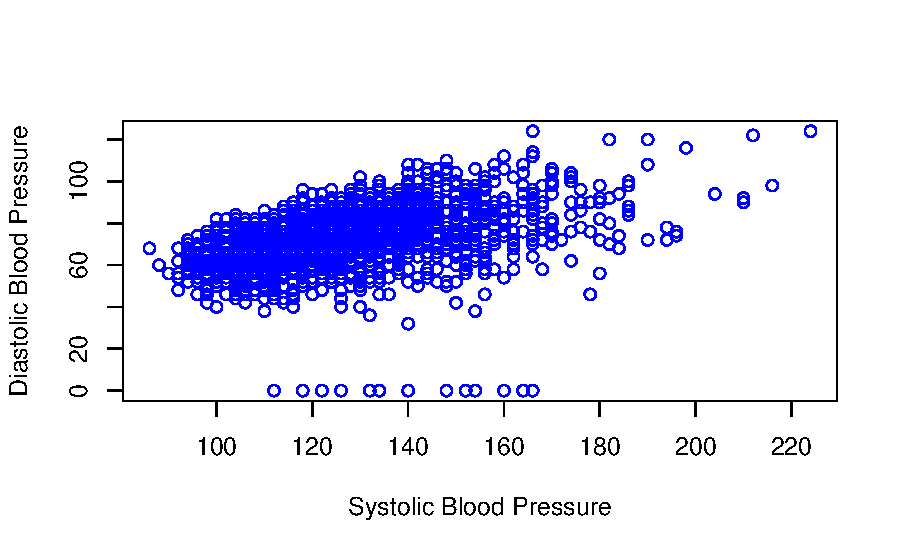
\includegraphics[width=1\textwidth,height=\textheight]{book/4_exploratory_analysis_files/figure-pdf/unnamed-chunk-17-1.pdf}

}

\end{figure}

The two measures of blood pressure look highly correlated. We can
calculate their Pearson and Spearman correlation using the
\texttt{cor()} function. The default method is the Pearson correlation,
but we can also calculate the Kendall or Spearman correlation by
specifying the method.

\begin{Shaded}
\begin{Highlighting}[]
\FunctionTok{cor}\NormalTok{(nhanes\_df}\SpecialCharTok{$}\NormalTok{SBP1, nhanes\_df}\SpecialCharTok{$}\NormalTok{DBP1)}
\CommentTok{\#\textgreater{} [1] 0.417}
\FunctionTok{cor}\NormalTok{(nhanes\_df}\SpecialCharTok{$}\NormalTok{SBP1, nhanes\_df}\SpecialCharTok{$}\NormalTok{DBP1, }\AttributeTok{method=}\StringTok{"spearman"}\NormalTok{)}
\CommentTok{\#\textgreater{} [1] 0.471}
\end{Highlighting}
\end{Shaded}

We may also want to add some extra information to our plot above. This
time, instead of specifying the color manually, we use the column
\texttt{hyp}, an indicator for hypertension, to specify the color. We
have to make sure this vector is a factor for R to color by group.
Additionally, we add a blue vertical and horizontal line using the
\texttt{abline()} function to mark cutoffs for hypertension. Even though
this function is called after \texttt{plot()}, the lines are
automatically added to the current plot. We can see that most of those
with hypertension have systolic or diastolic blood pressure measurements
above this threshold.

\begin{Shaded}
\begin{Highlighting}[]
\FunctionTok{plot}\NormalTok{(nhanes\_df}\SpecialCharTok{$}\NormalTok{SBP1, nhanes\_df}\SpecialCharTok{$}\NormalTok{DBP1, }\AttributeTok{col=}\FunctionTok{as.factor}\NormalTok{(nhanes\_df}\SpecialCharTok{$}\NormalTok{HYP), }
     \AttributeTok{xlab=}\StringTok{"Systolic Blood Pressure"}\NormalTok{,}
     \AttributeTok{ylab=}\StringTok{"Diastolic Blood Pressure"}\NormalTok{)}
\FunctionTok{abline}\NormalTok{(}\AttributeTok{v=}\DecValTok{130}\NormalTok{, }\AttributeTok{col=}\StringTok{"blue"}\NormalTok{)}
\FunctionTok{abline}\NormalTok{(}\AttributeTok{h=}\DecValTok{80}\NormalTok{, }\AttributeTok{col=}\StringTok{"blue"}\NormalTok{)}
\end{Highlighting}
\end{Shaded}

\begin{figure}[H]

{\centering 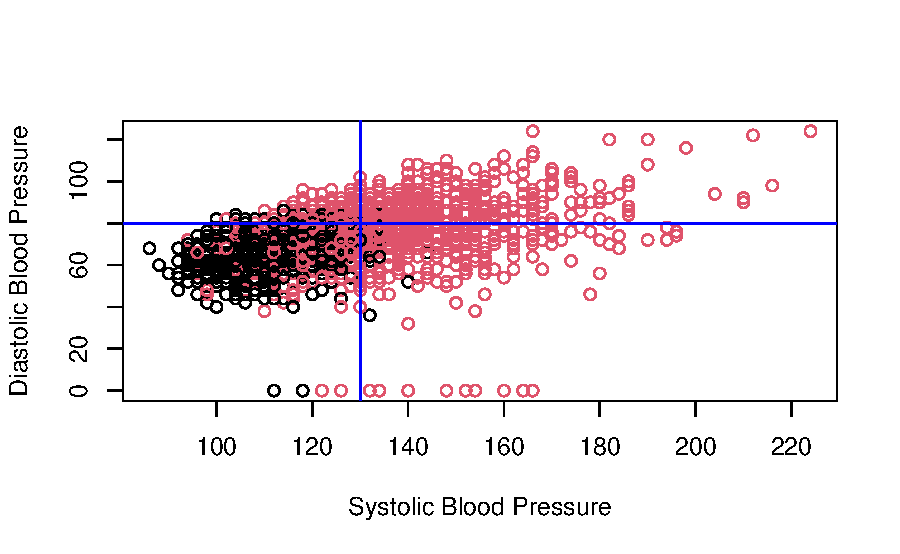
\includegraphics[width=1\textwidth,height=\textheight]{book/4_exploratory_analysis_files/figure-pdf/unnamed-chunk-19-1.pdf}

}

\end{figure}

The plots above are all displayed as a single figure. If we want to
display multiple plots next to each other, we can specify the graphical
parameters using the \texttt{par()} function by updating the argument
\texttt{mfrow=c(nrow,\ ncol)} with the number of columns and rows we
would like to use for our figures. Below, we use this to display the
distribution of log blood lead level between those with and without
hypertension next to the plot from above.

\begin{Shaded}
\begin{Highlighting}[]
\FunctionTok{par}\NormalTok{(}\AttributeTok{mfrow=}\FunctionTok{c}\NormalTok{(}\DecValTok{1}\NormalTok{,}\DecValTok{2}\NormalTok{))}

\CommentTok{\# boxplot}
\FunctionTok{boxplot}\NormalTok{(}\FunctionTok{log}\NormalTok{(LEAD)}\SpecialCharTok{\textasciitilde{}}\NormalTok{HYP, }\AttributeTok{data=}\NormalTok{nhanes\_df, }\AttributeTok{xlab=}\StringTok{"Hypertension"}\NormalTok{, }
        \AttributeTok{ylab=}\StringTok{"Log Blood Lead Level"}\NormalTok{)}

\CommentTok{\# scatterplot}
\FunctionTok{plot}\NormalTok{(nhanes\_df}\SpecialCharTok{$}\NormalTok{SBP1, nhanes\_df}\SpecialCharTok{$}\NormalTok{DBP1, }\AttributeTok{col=}\FunctionTok{as.factor}\NormalTok{(nhanes\_df}\SpecialCharTok{$}\NormalTok{HYP), }
     \AttributeTok{xlab=}\StringTok{"Systolic Blood Pressure"}\NormalTok{,}
     \AttributeTok{ylab=}\StringTok{"Diastolic Blood Pressure"}\NormalTok{)}
\FunctionTok{abline}\NormalTok{(}\AttributeTok{v=}\DecValTok{130}\NormalTok{, }\AttributeTok{col=}\StringTok{"blue"}\NormalTok{)}
\FunctionTok{abline}\NormalTok{(}\AttributeTok{h=}\DecValTok{80}\NormalTok{, }\AttributeTok{col=}\StringTok{"blue"}\NormalTok{)}
\end{Highlighting}
\end{Shaded}

\begin{figure}[H]

{\centering 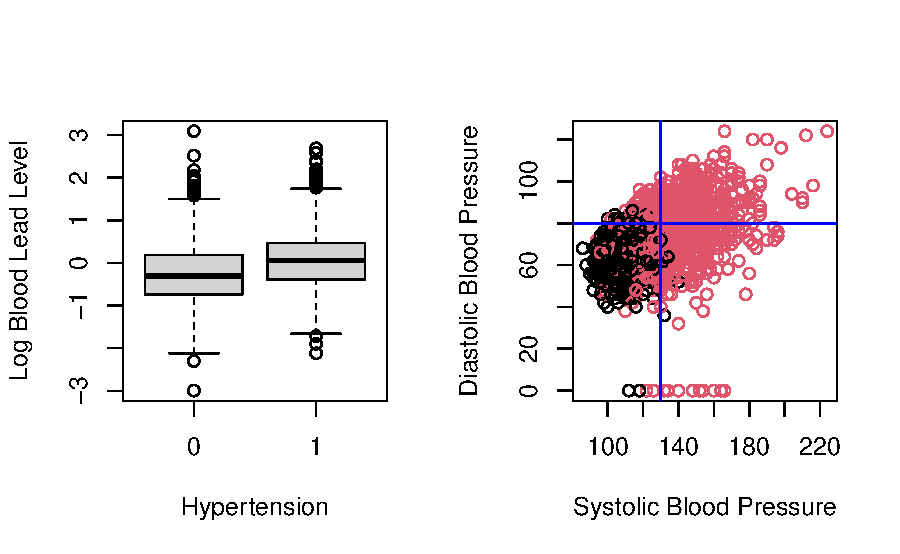
\includegraphics[width=1\textwidth,height=\textheight]{book/4_exploratory_analysis_files/figure-pdf/unnamed-chunk-20-1.pdf}

}

\end{figure}

We then reset to only display a single plot for future images using the
\texttt{par()} function again.

\begin{Shaded}
\begin{Highlighting}[]
\FunctionTok{par}\NormalTok{(}\AttributeTok{mfrow=}\FunctionTok{c}\NormalTok{(}\DecValTok{1}\NormalTok{,}\DecValTok{1}\NormalTok{))}
\end{Highlighting}
\end{Shaded}

\hypertarget{practice-question-7}{%
\subsection{Practice Question}\label{practice-question-7}}

Recreate the three boxplots in Figure~\ref{fig-pq2} (one for each
education level) of income by BMI category and arrange them next to each
other using the par() function.

\begin{figure}

{\centering 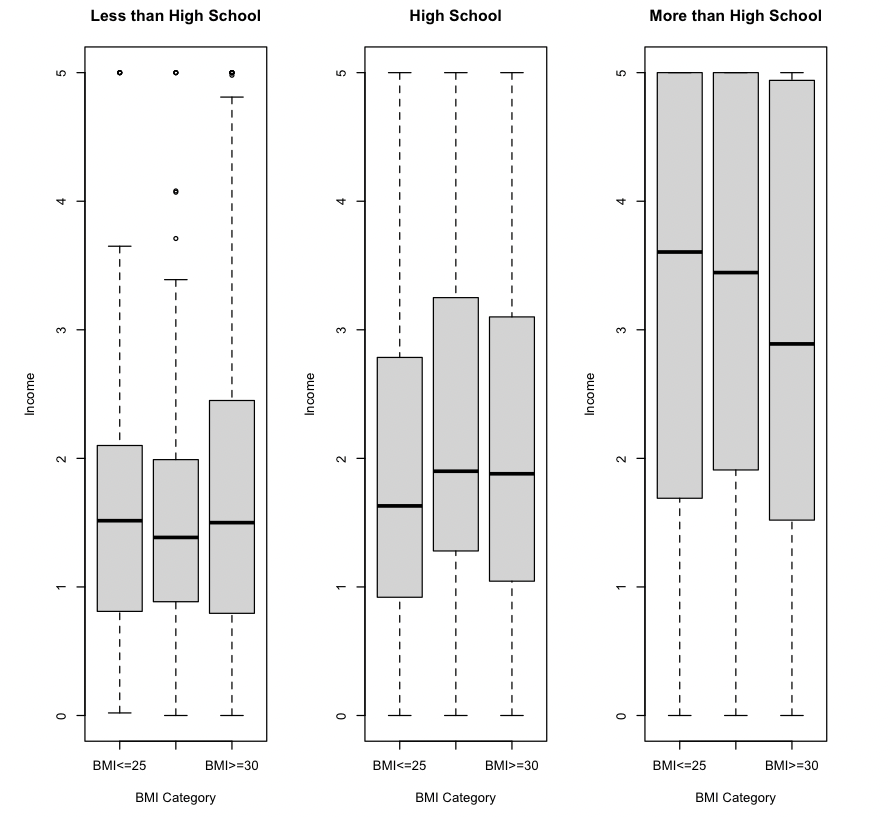
\includegraphics[width=4.16667in,height=\textheight]{book/images/4-practicequestion2answer.png}

}

\caption{\label{fig-pq2}Box Plot Example.}

\end{figure}

\begin{Shaded}
\begin{Highlighting}[]
\CommentTok{\# Insert your solution here:}
\end{Highlighting}
\end{Shaded}

\hypertarget{autogenerated-plots}{%
\section{Autogenerated Plots}\label{autogenerated-plots}}

Above, we learned some new functions for visualizing the relationship
between columns. The \textbf{GGally} package (Schloerke et al. 2021)
contains some useful functions for looking at multiple univariate and
bivariate relationships at the same time, such as the \texttt{ggpairs()}
function. \texttt{ggpairs()} takes the data as its first argument. By
default, it will plot the pairwise distributions for all columns, but we
can also specify to only select a subset of columns using the
\texttt{columns} argument. You can see below that it plots bar plots and
density plots for each univariate sample distribution. It then plots the
bivariate distributions and calculates the Pearson correlation for all
pairs of continuous columns. That's a lot of information!

\begin{Shaded}
\begin{Highlighting}[]
\FunctionTok{ggpairs}\NormalTok{(nhanes\_df, }\AttributeTok{columns =} \FunctionTok{c}\NormalTok{(}\StringTok{"SEX"}\NormalTok{, }\StringTok{"AGE"}\NormalTok{, }\StringTok{"LEAD"}\NormalTok{, }\StringTok{"SBP1"}\NormalTok{, }\StringTok{"DBP1"}\NormalTok{))}
\end{Highlighting}
\end{Shaded}

\begin{figure}[H]

{\centering 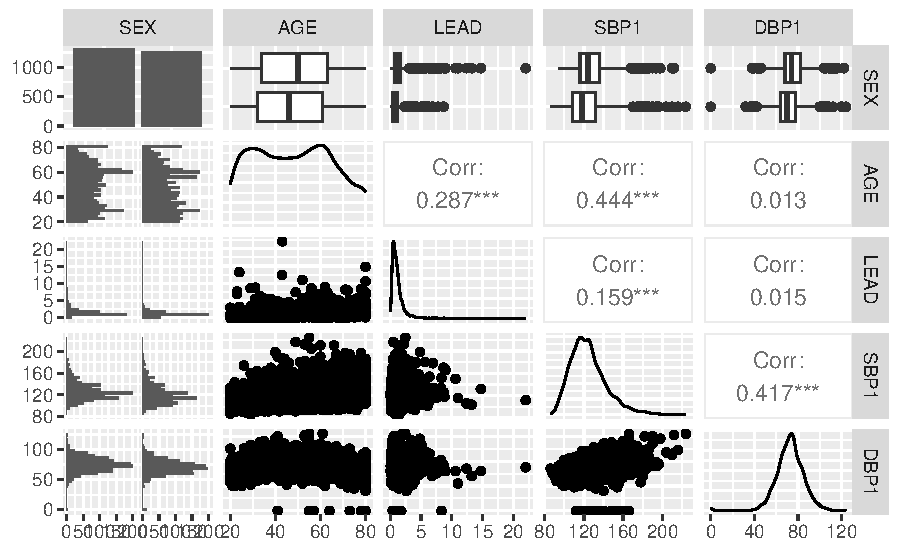
\includegraphics[width=1\textwidth,height=\textheight]{book/4_exploratory_analysis_files/figure-pdf/unnamed-chunk-23-1.pdf}

}

\end{figure}

Another useful function in this package is the \texttt{ggcorr()}
function: this function takes in a data frame with only numeric columns
and displays the correlation between all pairs of columns, where the
color of each grid cell indicates the strength of the correlation. The
additional argument \texttt{label=TRUE} prints the actual correlation
value on each grid cell. This is a useful way to identify pairs of
strongly correlated columns.

\begin{Shaded}
\begin{Highlighting}[]
\NormalTok{nhanes\_cont }\OtherTok{\textless{}{-}}\NormalTok{ nhanes\_df[,}\FunctionTok{c}\NormalTok{(}\StringTok{"AGE"}\NormalTok{, }\StringTok{"LEAD"}\NormalTok{, }\StringTok{"SBP1"}\NormalTok{, }\StringTok{"DBP1"}\NormalTok{)]}
\FunctionTok{ggcorr}\NormalTok{(nhanes\_cont, }\AttributeTok{label=}\ConstantTok{TRUE}\NormalTok{)}
\end{Highlighting}
\end{Shaded}

\begin{figure}[H]

{\centering 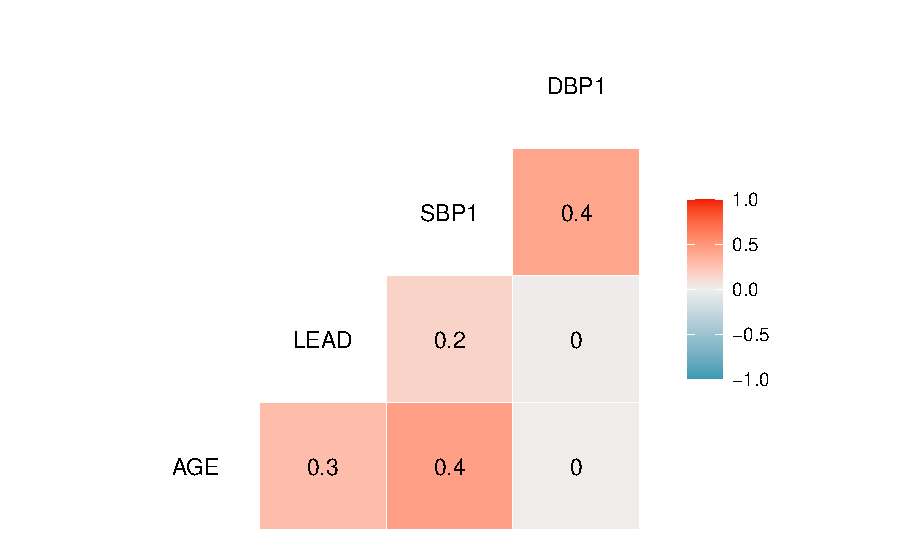
\includegraphics[width=1\textwidth,height=\textheight]{book/4_exploratory_analysis_files/figure-pdf/unnamed-chunk-24-1.pdf}

}

\end{figure}

\hypertarget{tables}{%
\section{Tables}\label{tables}}

Another useful way to display information about your data is through
tables. For example, it is standard practice in articles to have the
first table in the paper give information about the study sample, such
as the mean and standard deviation for all continuous columns and the
proportions for categorical columns. The \textbf{gt} package (Iannone et
al. 2023) is designed to create polished tables that can include
footnotes, titles, column labels, etc. The \textbf{gtsummary} package
(Sjoberg et al. 2023) is an extension of this package that can create
summary tables. We will focus on the latter but come back to creating
nice tables in Chapter~\ref{sec-rmarkdown}.

To start, we create a gt object (a special type of table) of the first
six rows of our data using the \texttt{gt()} function. You can see the
difference in the formatting as opposed to printing the data.

\begin{Shaded}
\begin{Highlighting}[]
\FunctionTok{gt}\NormalTok{(}\FunctionTok{head}\NormalTok{(nhanes\_df[, }\FunctionTok{c}\NormalTok{(}\StringTok{"ID"}\NormalTok{, }\StringTok{"AGE"}\NormalTok{, }\StringTok{"SEX"}\NormalTok{, }\StringTok{"RACE"}\NormalTok{)])) }
\end{Highlighting}
\end{Shaded}

\begin{longtable*}{rrcc}
\toprule
ID & AGE & SEX & RACE \\ 
\midrule
93711 & 56 & Male & Other Race \\ 
93713 & 67 & Male & Non-Hispanic White \\ 
93716 & 61 & Male & Other Race \\ 
93717 & 22 & Male & Non-Hispanic White \\ 
93721 & 60 & Female & Mexican American \\ 
93722 & 60 & Female & Non-Hispanic White \\ 
\bottomrule
\end{longtable*}

We will now show you how to use the \texttt{tbl\_summary()} function in
the \textbf{gtsummary} package. The first argument to this function is
again the data frame. By default, this function will summarize all the
columns in the data. Instead, we use the \texttt{include} argument to
specify a list of columns to include. We then pipe this result to
\texttt{as\_gt()} which creates a gt table from the summary output.
Again, we then need to pass this to \texttt{gt:::as.tags.gt\_tbl()} to
display this table as HTML within a Jupyter notebook. Note that the
table computes the total number of observations and the proportions for
categorical columns and the median and interquartile range for
continuous columns.

\begin{Shaded}
\begin{Highlighting}[]
\FunctionTok{tbl\_summary}\NormalTok{(nhanes\_df, }\AttributeTok{include=} \FunctionTok{c}\NormalTok{(}\StringTok{"SEX"}\NormalTok{, }\StringTok{"RACE"}\NormalTok{, }\StringTok{"AGE"}\NormalTok{, }\StringTok{"EDUCATION"}\NormalTok{, }\StringTok{"SMOKE"}\NormalTok{,}
                                  \StringTok{"BMI\_CAT"}\NormalTok{, }\StringTok{"LEAD"}\NormalTok{, }\StringTok{"SBP1"}\NormalTok{, }\StringTok{"DBP1"}\NormalTok{, }\StringTok{"HYP"}\NormalTok{)) }\SpecialCharTok{\%\textgreater{}\%} 
  \FunctionTok{as\_gt}\NormalTok{() }
\end{Highlighting}
\end{Shaded}

\setlength{\LTpost}{0mm}
\begin{longtable*}{lc}
\toprule
\textbf{Characteristic} & \textbf{N = 2,584}\textsuperscript{\textit{1}} \\ 
\midrule
SEX &  \\ 
    Male & 1,310 (51\%) \\ 
    Female & 1,274 (49\%) \\ 
RACE &  \\ 
    Mexican American & 358 (14\%) \\ 
    Other Hispanic & 225 (8.7\%) \\ 
    Non-Hispanic White & 992 (38\%) \\ 
    Non-Hispanic Black & 568 (22\%) \\ 
    Other Race & 441 (17\%) \\ 
AGE & 48 (33, 62) \\ 
EDUCATION &  \\ 
    LessThanHS & 373 (14\%) \\ 
    HS & 593 (23\%) \\ 
    MoreThanHS & 1,618 (63\%) \\ 
SMOKE &  \\ 
    NeverSmoke & 1,411 (55\%) \\ 
    QuitSmoke & 631 (24\%) \\ 
    StillSmoke & 542 (21\%) \\ 
BMI\_CAT &  \\ 
    BMI<=25 & 663 (26\%) \\ 
    25<BMI<30 & 808 (31\%) \\ 
    BMI>=30 & 1,113 (43\%) \\ 
LEAD & 0.93 (0.56, 1.44) \\ 
SBP1 & 122 (112, 134) \\ 
DBP1 & 72 (66, 80) \\ 
HYP & 1,451 (56\%) \\ 
\bottomrule
\end{longtable*}
\begin{minipage}{\linewidth}
\textsuperscript{\textit{1}}n (\%); Median (IQR)\\
\end{minipage}

We can update our table by changing some of its arguments. This time, we
specify that we want to stratify our table by hypertension status so
that the table summarizes the data by this grouping. Additionally, we
change how continuous columns are summarized by specifying that we want
to report the mean and standard deviation instead of the median and
interquartile range. We do this using the \texttt{statistic} argument.
The documentation for the \texttt{tbl\_summary()} function can help you
format this argument depending on which statistics you would like to
display.

\begin{Shaded}
\begin{Highlighting}[]
\FunctionTok{tbl\_summary}\NormalTok{(nhanes\_df, }\AttributeTok{include=} \FunctionTok{c}\NormalTok{(}\StringTok{"SEX"}\NormalTok{, }\StringTok{"RACE"}\NormalTok{, }\StringTok{"AGE"}\NormalTok{, }\StringTok{"EDUCATION"}\NormalTok{, }\StringTok{"SMOKE"}\NormalTok{,}
                                  \StringTok{"BMI\_CAT"}\NormalTok{, }\StringTok{"LEAD"}\NormalTok{, }\StringTok{"SBP1"}\NormalTok{, }\StringTok{"DBP1"}\NormalTok{, }\StringTok{"HYP"}\NormalTok{),}
           \AttributeTok{by =} \StringTok{"HYP"}\NormalTok{, }\AttributeTok{statistic =} \FunctionTok{list}\NormalTok{(}\FunctionTok{all\_continuous}\NormalTok{() }\SpecialCharTok{\textasciitilde{}} \StringTok{"\{mean\} (\{sd\})"}\NormalTok{)) }\SpecialCharTok{\%\textgreater{}\%} 
  \FunctionTok{as\_gt}\NormalTok{() }
\end{Highlighting}
\end{Shaded}

\setlength{\LTpost}{0mm}
\begin{longtable*}{lcc}
\toprule
\textbf{Characteristic} & \textbf{0}, N = 1,133\textsuperscript{\textit{1}} & \textbf{1}, N = 1,451\textsuperscript{\textit{1}} \\ 
\midrule
SEX &  &  \\ 
    Male & 472 (42\%) & 838 (58\%) \\ 
    Female & 661 (58\%) & 613 (42\%) \\ 
RACE &  &  \\ 
    Mexican American & 186 (16\%) & 172 (12\%) \\ 
    Other Hispanic & 104 (9.2\%) & 121 (8.3\%) \\ 
    Non-Hispanic White & 429 (38\%) & 563 (39\%) \\ 
    Non-Hispanic Black & 203 (18\%) & 365 (25\%) \\ 
    Other Race & 211 (19\%) & 230 (16\%) \\ 
AGE & 40 (15) & 55 (16) \\ 
EDUCATION &  &  \\ 
    LessThanHS & 151 (13\%) & 222 (15\%) \\ 
    HS & 250 (22\%) & 343 (24\%) \\ 
    MoreThanHS & 732 (65\%) & 886 (61\%) \\ 
SMOKE &  &  \\ 
    NeverSmoke & 678 (60\%) & 733 (51\%) \\ 
    QuitSmoke & 220 (19\%) & 411 (28\%) \\ 
    StillSmoke & 235 (21\%) & 307 (21\%) \\ 
BMI\_CAT &  &  \\ 
    BMI<=25 & 392 (35\%) & 271 (19\%) \\ 
    25<BMI<30 & 351 (31\%) & 457 (31\%) \\ 
    BMI>=30 & 390 (34\%) & 723 (50\%) \\ 
LEAD & 1.03 (1.15) & 1.37 (1.25) \\ 
SBP1 & 112 (10) & 134 (18) \\ 
DBP1 & 67 (9) & 77 (14) \\ 
\bottomrule
\end{longtable*}
\begin{minipage}{\linewidth}
\textsuperscript{\textit{1}}n (\%); Mean (SD)\\
\end{minipage}

Outside of the \textbf{gt} and \textbf{gtsummary} packages, another
common package used to create summary tables is the \textbf{tableone}
package (Yoshida and Bartel 2022), which is not covered in this book.

\hypertarget{exercises-2}{%
\section{Exercises}\label{exercises-2}}

For these exercises, we will continue using the \texttt{nhanes\_df}
data.

\begin{enumerate}
\def\labelenumi{\arabic{enumi}.}
\item
  Using both numerical and graphical summaries, describe the
  distribution of the first diastolic blood pressure reading
  \texttt{DBP1}among study participants. Then, create a column called
  \texttt{INCOME\_CAT} with two categories: ``low'' for those whose
  income is at most 2 and ``not low'' otherwise and examine the
  bivariate distribution of \texttt{DBP1} and \texttt{INCOME\_CAT}.
  Arrange the two plots next to each other. What do you notice?
\item
  Subset the data to adults between the ages of 20 and 55. Then, explore
  how blood pressure varies by age and gender among this age group. Is
  there a visible trend in blood pressure with increasing age among
  either sex?
\item
  For males between the ages of 50-59, compare blood pressure across
  race as reported in the race column. Then, create a summary table
  stratified by the race column and report the mean, standard deviation,
  minimum and maximum values for all continuous columns.
\item
  Recreate the the plots in Figure~\ref{fig-q41} and
  Figure~\ref{fig-q42}. Based on what you see, how do you expect blood
  lead levels to change by year? Check your answer to the previous
  question by plotting these two columns against each other.
\end{enumerate}

\begin{figure}

{\centering 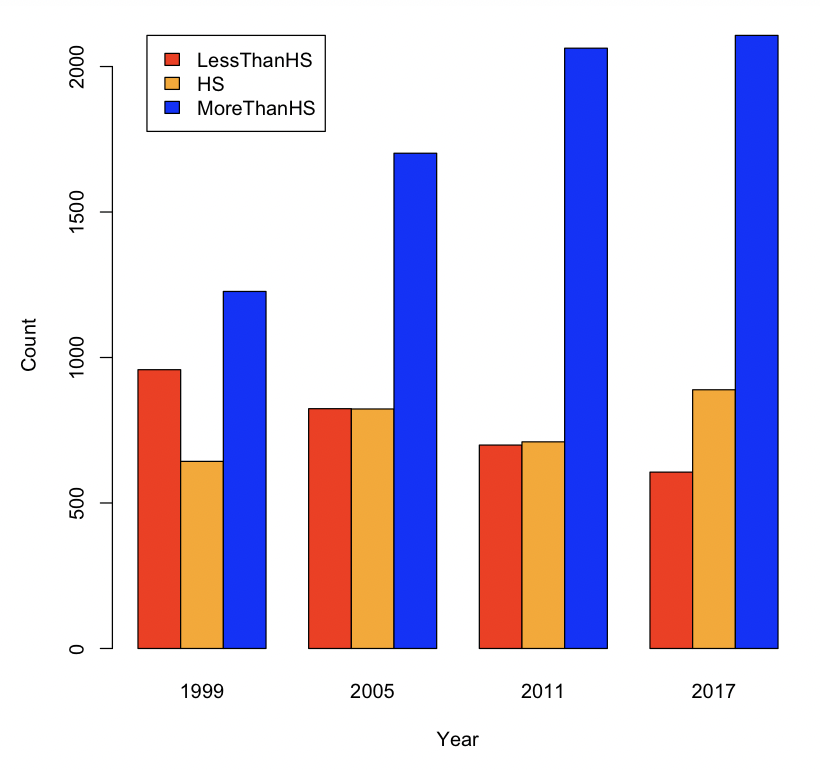
\includegraphics[width=2.08333in,height=\textheight]{book/images/4-exercise4plot1.png}

}

\caption{\label{fig-q41}Education Levels Over Time.}

\end{figure}

\begin{figure}

{\centering 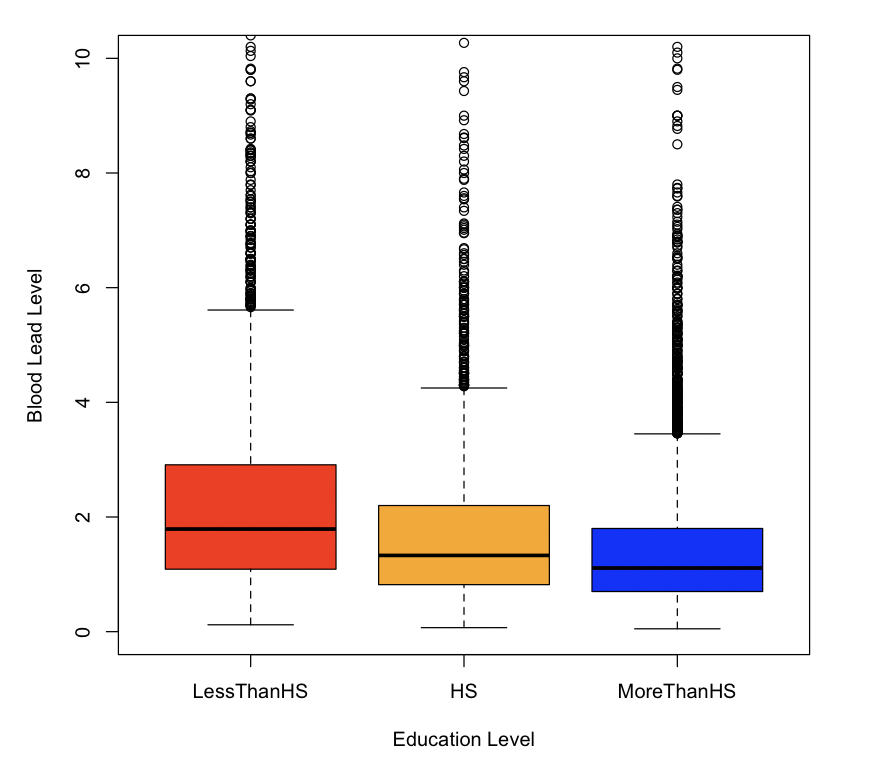
\includegraphics[width=2.08333in,height=\textheight]{book/images/4-exercise4plot2.png}

}

\caption{\label{fig-q42}Blood Lead Level by Education Level.}

\end{figure}

\bookmarksetup{startatroot}

\hypertarget{sec-transformations-summaries}{%
\chapter{Data Transformations and
Summaries}\label{sec-transformations-summaries}}

In this chapter, we will introduce the \textbf{dyplr} package (Wickham
et al. 2023), which is part of the \textbf{tidyverse} group of packages,
to expand our tools in exploring and transforming our data. We will
learn how to do some basic manipulations of data (e.g.~adding or
removing columns, filtering data, arranging by one or multiple columns)
as well as how to summarize data (e.g.~grouping by values, calculating
summary statistics). We will also practice combining these operations
using the pipe operator \texttt{\%\textgreater{}\%}. We will use the
same sample of the National Health and Nutrition Examination Survey
(Disease Control and (CDC) 1999-2018) as in
Chapter~\ref{sec-exploratory}.

\begin{Shaded}
\begin{Highlighting}[]
\FunctionTok{library}\NormalTok{(HDSinRdata)}
\FunctionTok{library}\NormalTok{(tidyverse)}
\FunctionTok{data}\NormalTok{(NHANESsample)}
\end{Highlighting}
\end{Shaded}

\hypertarget{tibbles-and-data-frames}{%
\section{Tibbles and Data Frames}\label{tibbles-and-data-frames}}

Take a look at the class of \texttt{NHANESsample}. As we might expect,
the data is stored as a data frame.

\begin{Shaded}
\begin{Highlighting}[]
\FunctionTok{class}\NormalTok{(NHANESsample)}
\CommentTok{\#\textgreater{} [1] "data.frame"}
\end{Highlighting}
\end{Shaded}

However, the tidyverse also works with another data structure called a
\textbf{tibble}. A \textbf{tibble} has all the properties of data frames
that we have learned so far, but they are a more modern version of a
data frame. To convert our data to this data structure we use the
\texttt{as\_tibble()} function. In practice, there are only very slight
difference between the two data structures, and you generally do not
need to convert data frames to tibbles. Below we convert our data from a
data frame to a tibble and print the head of the data before converting
it back to a data frame and repeating. You can see the two structures
have a slightly different print statement but are otherwise very
similar.

\begin{Shaded}
\begin{Highlighting}[]
\NormalTok{nhanes\_df }\OtherTok{\textless{}{-}} \FunctionTok{as\_tibble}\NormalTok{(NHANESsample)}
\FunctionTok{print}\NormalTok{(}\FunctionTok{head}\NormalTok{(nhanes\_df))}
\CommentTok{\#\textgreater{} \# A tibble: 6 x 21}
\CommentTok{\#\textgreater{}      ID   AGE SEX   RACE              EDUCATION INCOME SMOKE  YEAR  LEAD BMI\_CAT}
\CommentTok{\#\textgreater{}   \textless{}dbl\textgreater{} \textless{}dbl\textgreater{} \textless{}fct\textgreater{} \textless{}fct\textgreater{}             \textless{}fct\textgreater{}      \textless{}dbl\textgreater{} \textless{}fct\textgreater{} \textless{}dbl\textgreater{} \textless{}dbl\textgreater{} \textless{}fct\textgreater{}  }
\CommentTok{\#\textgreater{} 1     2    77 Male  Non{-}Hispanic Whi\textasciitilde{} MoreThan\textasciitilde{}   5    Neve\textasciitilde{}  1999   5   BMI\textless{}=25}
\CommentTok{\#\textgreater{} 2     5    49 Male  Non{-}Hispanic Whi\textasciitilde{} MoreThan\textasciitilde{}   5    Quit\textasciitilde{}  1999   1.6 25\textless{}BMI\textasciitilde{}}
\CommentTok{\#\textgreater{} 3    12    37 Male  Non{-}Hispanic Whi\textasciitilde{} MoreThan\textasciitilde{}   4.93 Neve\textasciitilde{}  1999   2.4 BMI\textgreater{}=30}
\CommentTok{\#\textgreater{} 4    13    70 Male  Mexican American  LessThan\textasciitilde{}   1.07 Quit\textasciitilde{}  1999   1.6 25\textless{}BMI\textasciitilde{}}
\CommentTok{\#\textgreater{} 5    14    81 Male  Non{-}Hispanic Whi\textasciitilde{} LessThan\textasciitilde{}   2.67 Stil\textasciitilde{}  1999   5.5 25\textless{}BMI\textasciitilde{}}
\CommentTok{\#\textgreater{} \# i 1 more row}
\CommentTok{\#\textgreater{} \# i 11 more variables: LEAD\_QUANTILE \textless{}fct\textgreater{}, HYP \textless{}dbl\textgreater{}, ALC \textless{}chr\textgreater{}, DBP1 \textless{}dbl\textgreater{},}
\CommentTok{\#\textgreater{} \#   DBP2 \textless{}dbl\textgreater{}, DBP3 \textless{}dbl\textgreater{}, DBP4 \textless{}dbl\textgreater{}, SBP1 \textless{}dbl\textgreater{}, SBP2 \textless{}dbl\textgreater{}, SBP3 \textless{}dbl\textgreater{},}
\CommentTok{\#\textgreater{} \#   SBP4 \textless{}dbl\textgreater{}}
\end{Highlighting}
\end{Shaded}

\begin{Shaded}
\begin{Highlighting}[]
\NormalTok{nhanes\_df }\OtherTok{\textless{}{-}} \FunctionTok{as.data.frame}\NormalTok{(nhanes\_df)}
\FunctionTok{print}\NormalTok{(}\FunctionTok{head}\NormalTok{(nhanes\_df))}
\CommentTok{\#\textgreater{}   ID AGE    SEX               RACE  EDUCATION INCOME      SMOKE YEAR LEAD}
\CommentTok{\#\textgreater{} 1  2  77   Male Non{-}Hispanic White MoreThanHS   5.00 NeverSmoke 1999  5.0}
\CommentTok{\#\textgreater{} 2  5  49   Male Non{-}Hispanic White MoreThanHS   5.00  QuitSmoke 1999  1.6}
\CommentTok{\#\textgreater{} 3 12  37   Male Non{-}Hispanic White MoreThanHS   4.93 NeverSmoke 1999  2.4}
\CommentTok{\#\textgreater{} 4 13  70   Male   Mexican American LessThanHS   1.07  QuitSmoke 1999  1.6}
\CommentTok{\#\textgreater{} 5 14  81   Male Non{-}Hispanic White LessThanHS   2.67 StillSmoke 1999  5.5}
\CommentTok{\#\textgreater{} 6 15  38 Female Non{-}Hispanic White MoreThanHS   4.52 StillSmoke 1999  1.5}
\CommentTok{\#\textgreater{}     BMI\_CAT LEAD\_QUANTILE HYP ALC DBP1 DBP2 DBP3 DBP4 SBP1 SBP2 SBP3 SBP4}
\CommentTok{\#\textgreater{} 1   BMI\textless{}=25            Q4   0 Yes   58   56   56   NA  106   98   98   NA}
\CommentTok{\#\textgreater{} 2 25\textless{}BMI\textless{}30            Q3   1 Yes   82   84   82   NA  122  122  122   NA}
\CommentTok{\#\textgreater{} 3   BMI\textgreater{}=30            Q4   1 Yes  108   98  100   NA  182  172  176   NA}
\CommentTok{\#\textgreater{} 4 25\textless{}BMI\textless{}30            Q3   1 Yes   78   62   70   NA  140  130  130   NA}
\CommentTok{\#\textgreater{} 5 25\textless{}BMI\textless{}30            Q4   1 Yes   56   NA   58   64  142   NA  134  138}
\CommentTok{\#\textgreater{} 6 25\textless{}BMI\textless{}30            Q3   0 Yes   68   68   70   NA  106  112  106   NA}
\end{Highlighting}
\end{Shaded}

We mention tibbles here since some functions in the \textbf{tidyverse}
package convert data frames to tibbles in their output. In particular,
when we summarize over groups below we can expect a tibble to be
returned. It is useful to be aware that our data may change data
structure with such functions and to know that we can always convert
back if needed.

\hypertarget{subsetting-data}{%
\section{Subsetting Data}\label{subsetting-data}}

In earlier chapters, we have seen how to select and filter data using
row and column indices as well as using the \texttt{subset()} function.
The \textbf{dplyr} package has its own functions that are useful to
subset the data. The \texttt{select()} function allows us to select a
subset of columns: this function takes in the data frame (or tibble) and
the names or indices of the columns we want to select. For example, if
we only wanted to select the variables for race and blood lead level, we
could specify these two columns. To display the result of this
selection, we use the pipe operator \texttt{\%\textgreater{}\%}. Recall
that this takes the result on the left hand side and passes it as the
first argument to the function on the right hand side. The output below
shows that there are only two columns in the filtered data.

\begin{Shaded}
\begin{Highlighting}[]
\FunctionTok{select}\NormalTok{(nhanes\_df, }\FunctionTok{c}\NormalTok{(RACE, LEAD)) }\SpecialCharTok{\%\textgreater{}\%} \FunctionTok{head}\NormalTok{()}
\CommentTok{\#\textgreater{}                 RACE LEAD}
\CommentTok{\#\textgreater{} 1 Non{-}Hispanic White  5.0}
\CommentTok{\#\textgreater{} 2 Non{-}Hispanic White  1.6}
\CommentTok{\#\textgreater{} 3 Non{-}Hispanic White  2.4}
\CommentTok{\#\textgreater{} 4   Mexican American  1.6}
\CommentTok{\#\textgreater{} 5 Non{-}Hispanic White  5.5}
\CommentTok{\#\textgreater{} 6 Non{-}Hispanic White  1.5}
\end{Highlighting}
\end{Shaded}

The \texttt{select()} function can also be used to \emph{remove} columns
by adding a negative sign in front of the vector of column names in its
arguments. For example, below we keep all columns except \texttt{ID} and
\texttt{LEAD\_QUANTILE}. Note that in this case we have saved the
selected data back to our data frame \texttt{nhanes\_df}. Additionally,
this time we used a pipe operator to pipe the data to the select
function itself.

\begin{Shaded}
\begin{Highlighting}[]
\NormalTok{nhanes\_df }\OtherTok{\textless{}{-}}\NormalTok{ nhanes\_df }\SpecialCharTok{\%\textgreater{}\%} \FunctionTok{select}\NormalTok{(}\SpecialCharTok{{-}}\FunctionTok{c}\NormalTok{(ID, LEAD\_QUANTILE))}
\FunctionTok{names}\NormalTok{(nhanes\_df)}
\CommentTok{\#\textgreater{}  [1] "AGE"       "SEX"       "RACE"      "EDUCATION" "INCOME"    "SMOKE"    }
\CommentTok{\#\textgreater{}  [7] "YEAR"      "LEAD"      "BMI\_CAT"   "HYP"       "ALC"       "DBP1"     }
\CommentTok{\#\textgreater{} [13] "DBP2"      "DBP3"      "DBP4"      "SBP1"      "SBP2"      "SBP3"     }
\CommentTok{\#\textgreater{} [19] "SBP4"}
\end{Highlighting}
\end{Shaded}

While \texttt{select()} allows us to choose a subset of columns, the
\texttt{filter()} function allows us to choose a subset of rows. The
\texttt{filter()} function takes a data frame as the first argument and
a vector of booleans as the second argument. This vector of booleans can
be generated using conditional statements as we used in
Chapter~\ref{sec-exploratory}. Below, we choose to filter the data to
only observations after 2008.

\begin{Shaded}
\begin{Highlighting}[]
\NormalTok{nhanes\_df\_recent }\OtherTok{\textless{}{-}}\NormalTok{ nhanes\_df }\SpecialCharTok{\%\textgreater{}\%} \FunctionTok{filter}\NormalTok{(YEAR }\SpecialCharTok{\textgreater{}=} \DecValTok{2008}\NormalTok{)}
\end{Highlighting}
\end{Shaded}

We can combine conditions by using multiple \texttt{filter} calls, by
creating a more complicated conditional statement using the \texttt{\&}
(and), \texttt{\textbar{}} (or), and \texttt{\%in\%} (in) operators, or
by separating the conditions with commas within filter. Below, we
demonstrate these three ways to filter the data to males between 2008
and 2012. Note that the \texttt{between()} function allows us to capture
the logic
\texttt{YEAR\ \textgreater{}=\ 2008\ \&\ YEAR\ \textless{}=\ 2012}.

\begin{Shaded}
\begin{Highlighting}[]
\CommentTok{\# Example 1: multiple filter calls}
\NormalTok{nhanes\_df\_males1 }\OtherTok{\textless{}{-}}\NormalTok{ nhanes\_df }\SpecialCharTok{\%\textgreater{}\%}
  \FunctionTok{filter}\NormalTok{(YEAR }\SpecialCharTok{\textless{}=} \DecValTok{2012}\NormalTok{) }\SpecialCharTok{\%\textgreater{}\%}
  \FunctionTok{filter}\NormalTok{(YEAR }\SpecialCharTok{\textgreater{}=} \DecValTok{2008}\NormalTok{) }\SpecialCharTok{\%\textgreater{}\%}
  \FunctionTok{filter}\NormalTok{(SEX }\SpecialCharTok{==} \StringTok{"Male"}\NormalTok{)}

\CommentTok{\# Example 2: combine with \& operator}
\NormalTok{nhanes\_df\_males2 }\OtherTok{\textless{}{-}}\NormalTok{ nhanes\_df }\SpecialCharTok{\%\textgreater{}\%}
  \FunctionTok{filter}\NormalTok{((YEAR }\SpecialCharTok{\textless{}=} \DecValTok{2012}\NormalTok{) }\SpecialCharTok{\&}\NormalTok{ (YEAR }\SpecialCharTok{\textgreater{}=} \DecValTok{2008}\NormalTok{) }\SpecialCharTok{\&}\NormalTok{ (SEX }\SpecialCharTok{==} \StringTok{"Male"}\NormalTok{))}

\CommentTok{\# Example 3: combine into one filter call with commas}
\NormalTok{nhanes\_df\_males3 }\OtherTok{\textless{}{-}}\NormalTok{ nhanes\_df }\SpecialCharTok{\%\textgreater{}\%}
  \FunctionTok{filter}\NormalTok{(}\FunctionTok{between}\NormalTok{(YEAR, }\DecValTok{2008}\NormalTok{, }\DecValTok{2012}\NormalTok{), SEX }\SpecialCharTok{==} \StringTok{"Male"}\NormalTok{)}
\end{Highlighting}
\end{Shaded}

The use of parentheses in the code above is especially important in
order to capture our desired logic. In all these examples, we broke our
code up into multiple lines, which makes it easier to read. A good rule
of thumb is to not go past 80 characters in a line, and R Studio
conveniently has a vertical gray line at this limit. To create a new
line, you can hit enter either after an operator
(e.g.~\texttt{\%\textgreater{}\%}, \texttt{+}, \texttt{\textbar{}}) or
within a set of unfinished brackets or parentheses. Either of these
breaks lets R know that your code is not finished yet.

Lastly, we can subset the data using the \texttt{slice()} function to
select a slice of rows by their index. The function takes in the data
set and a vector of indices. Below, we find the first and last rows of
the data.

\begin{Shaded}
\begin{Highlighting}[]
\FunctionTok{slice}\NormalTok{(nhanes\_df, }\FunctionTok{c}\NormalTok{(}\DecValTok{1}\NormalTok{, }\FunctionTok{nrow}\NormalTok{(nhanes\_df)))}
\CommentTok{\#\textgreater{}   AGE  SEX               RACE  EDUCATION INCOME      SMOKE YEAR LEAD BMI\_CAT}
\CommentTok{\#\textgreater{} 1  77 Male Non{-}Hispanic White MoreThanHS   5.00 NeverSmoke 1999  5.0 BMI\textless{}=25}
\CommentTok{\#\textgreater{} 2  38 Male Non{-}Hispanic White MoreThanHS   1.56 StillSmoke 2017  0.9 BMI\textgreater{}=30}
\CommentTok{\#\textgreater{}   HYP ALC DBP1 DBP2 DBP3 DBP4 SBP1 SBP2 SBP3 SBP4}
\CommentTok{\#\textgreater{} 1   0 Yes   58   56   56   NA  106   98   98   NA}
\CommentTok{\#\textgreater{} 2   1 Yes   98   92   98   NA  150  146  148   NA}
\end{Highlighting}
\end{Shaded}

A few other useful slice functions are \texttt{slice\_sample()},
\texttt{slice\_max()}, and \texttt{slice\_min()}. The first takes in an
argument \texttt{n} which specifies the number of \emph{random} rows to
sample from the data. For example, we could randomly sample 100 rows
from our data. The latter two allow us to specify a column through the
argument \texttt{order\_by} and return the \texttt{n} rows with either
the highest or lowest values in that column. Below we find the three
male observations from 2007 with the highest and lowest blood lead
levels and select a subset of columns to display.

\begin{Shaded}
\begin{Highlighting}[]
\CommentTok{\# three male observations with highest blood lead level in 2007}
\NormalTok{nhanes\_df }\SpecialCharTok{\%\textgreater{}\%}
  \FunctionTok{filter}\NormalTok{(YEAR }\SpecialCharTok{==} \DecValTok{2007}\NormalTok{, SEX }\SpecialCharTok{==} \StringTok{"Male"}\NormalTok{) }\SpecialCharTok{\%\textgreater{}\%}
  \FunctionTok{select}\NormalTok{(}\FunctionTok{c}\NormalTok{(RACE, EDUCATION, SMOKE, LEAD, SBP1, DBP1)) }\SpecialCharTok{\%\textgreater{}\%}
  \FunctionTok{slice\_max}\NormalTok{(}\AttributeTok{order\_by =}\NormalTok{ LEAD, }\AttributeTok{n=}\DecValTok{3}\NormalTok{)}
\CommentTok{\#\textgreater{}                 RACE  EDUCATION      SMOKE LEAD SBP1 DBP1}
\CommentTok{\#\textgreater{} 1 Non{-}Hispanic Black LessThanHS NeverSmoke 33.1  106   66}
\CommentTok{\#\textgreater{} 2     Other Hispanic LessThanHS StillSmoke 26.8  106   72}
\CommentTok{\#\textgreater{} 3     Other Hispanic LessThanHS StillSmoke 25.7  112   60}

\CommentTok{\# three male observations with lowest blood lead level in 2007}
\NormalTok{nhanes\_df }\SpecialCharTok{\%\textgreater{}\%}
  \FunctionTok{filter}\NormalTok{(YEAR }\SpecialCharTok{==} \DecValTok{2007}\NormalTok{, SEX }\SpecialCharTok{==} \StringTok{"Male"}\NormalTok{) }\SpecialCharTok{\%\textgreater{}\%}
  \FunctionTok{select}\NormalTok{(}\FunctionTok{c}\NormalTok{(RACE, EDUCATION, SMOKE, LEAD, SBP1, DBP1)) }\SpecialCharTok{\%\textgreater{}\%}
  \FunctionTok{slice\_min}\NormalTok{(}\AttributeTok{order\_by =}\NormalTok{ LEAD, }\AttributeTok{n=}\DecValTok{3}\NormalTok{)}
\CommentTok{\#\textgreater{}                 RACE  EDUCATION      SMOKE  LEAD SBP1 DBP1}
\CommentTok{\#\textgreater{} 1 Non{-}Hispanic White LessThanHS NeverSmoke 0.177  114   80}
\CommentTok{\#\textgreater{} 2     Other Hispanic LessThanHS  QuitSmoke 0.280  122   62}
\CommentTok{\#\textgreater{} 3   Mexican American MoreThanHS  QuitSmoke 0.320  112   66}
\end{Highlighting}
\end{Shaded}

\hypertarget{practice-question-8}{%
\subsection{Practice Question}\label{practice-question-8}}

Filter the data to only those with an education level of more than HS
who report alcohol use. Then, select only the diastolic blood pressure
variables and display the 4th and 10th rows. Your result should match
the result in Figure~\ref{fig-pq1}.

\begin{figure}

{\centering 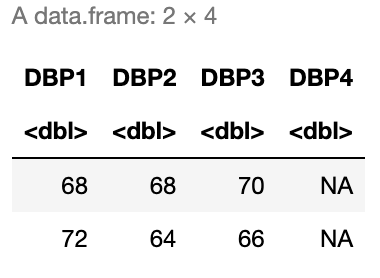
\includegraphics[width=2.08333in,height=\textheight]{book/images/5-practicequestion1answer.png}

}

\caption{\label{fig-pq1}Filtering and Selecting Data.}

\end{figure}

\begin{Shaded}
\begin{Highlighting}[]
\CommentTok{\# Insert your solution here:}
\end{Highlighting}
\end{Shaded}

\hypertarget{updating-rows-and-columns}{%
\section{Updating Rows and Columns}\label{updating-rows-and-columns}}

The next few functions we will look at will allow us to update the rows
and columns in our data. For example, the \texttt{rename()} function
allows us to change the names of columns. Below, we change the name of
\texttt{INCOME} to \texttt{PIR} since this variable is the poverty
income ratio and also update the name of \texttt{SMOKE} to be
\texttt{SMOKE\_STATUS}. When specifying these names, the new name is on
the left of the \texttt{=} and the old name is on the right.

\begin{Shaded}
\begin{Highlighting}[]
\NormalTok{nhanes\_df }\OtherTok{\textless{}{-}}\NormalTok{ nhanes\_df }\SpecialCharTok{\%\textgreater{}\%} \FunctionTok{rename}\NormalTok{(}\AttributeTok{PIR =}\NormalTok{ INCOME, }\AttributeTok{SMOKE\_STATUS =}\NormalTok{ SMOKE)}
\FunctionTok{names}\NormalTok{(nhanes\_df)}
\CommentTok{\#\textgreater{}  [1] "AGE"          "SEX"          "RACE"         "EDUCATION"    "PIR"         }
\CommentTok{\#\textgreater{}  [6] "SMOKE\_STATUS" "YEAR"         "LEAD"         "BMI\_CAT"      "HYP"         }
\CommentTok{\#\textgreater{} [11] "ALC"          "DBP1"         "DBP2"         "DBP3"         "DBP4"        }
\CommentTok{\#\textgreater{} [16] "SBP1"         "SBP2"         "SBP3"         "SBP4"}
\end{Highlighting}
\end{Shaded}

In the last chapter, we created a new variable called
\texttt{EVER\_SMOKE} based on the smoking status variable using the
\texttt{ifelse()} function. Recall that this function allows us to
specify a condition and then two alternative values based on whether we
meet or do not meet this condition. We see that there are about 15,000
subjects in our data who never smoked.

\begin{Shaded}
\begin{Highlighting}[]
\FunctionTok{ifelse}\NormalTok{(nhanes\_df}\SpecialCharTok{$}\NormalTok{SMOKE\_STATUS }\SpecialCharTok{==} \StringTok{"NeverSmoke"}\NormalTok{, }\StringTok{"No"}\NormalTok{, }\StringTok{"Yes"}\NormalTok{) }\SpecialCharTok{\%\textgreater{}\%} \FunctionTok{table}\NormalTok{()}
\CommentTok{\#\textgreater{} .}
\CommentTok{\#\textgreater{}    No   Yes }
\CommentTok{\#\textgreater{} 15087 16178}
\end{Highlighting}
\end{Shaded}

Another useful function from the tidyverse is the \texttt{case\_when()}
function, which is an extension of the \texttt{ifelse()} function but
allows to specify more than two cases. We demonstrate this function
below to show how we could relabel the levels of the
\texttt{SMOKE\_STATUS} column. For each condition, we use the right side
of the \texttt{\textasciitilde{}} to specify the value associated with a
TRUE for that condition.

\begin{Shaded}
\begin{Highlighting}[]
\FunctionTok{case\_when}\NormalTok{(nhanes\_df}\SpecialCharTok{$}\NormalTok{SMOKE\_STATUS }\SpecialCharTok{==} \StringTok{"NeverSmoke"} \SpecialCharTok{\textasciitilde{}} \StringTok{"Never Smoked"}\NormalTok{,}
\NormalTok{          nhanes\_df}\SpecialCharTok{$}\NormalTok{SMOKE\_STATUS }\SpecialCharTok{==} \StringTok{"QuitSmoke"} \SpecialCharTok{\textasciitilde{}} \StringTok{"Quit Smoking"}\NormalTok{,}
\NormalTok{          nhanes\_df}\SpecialCharTok{$}\NormalTok{SMOKE\_STATUS }\SpecialCharTok{==} \StringTok{"StillSmoke"} \SpecialCharTok{\textasciitilde{}} \StringTok{"Current Smoker"}\NormalTok{) }\SpecialCharTok{\%\textgreater{}\%} 
  \FunctionTok{table}\NormalTok{()}
\CommentTok{\#\textgreater{} .}
\CommentTok{\#\textgreater{} Current Smoker   Never Smoked   Quit Smoking }
\CommentTok{\#\textgreater{}           7317          15087           8861}
\end{Highlighting}
\end{Shaded}

Above, we did not store the columns we created. To do so, we could use
the \texttt{\$} operator or the \texttt{cbind()} function. The tidyverse
also includes an alternative function to add columns called
\texttt{mutate()}. This function takes in a data frame and a set of
columns with associated names to add to the data or update. In the
example below, we create the column \texttt{EVER\_SMOKE} and update the
column \texttt{SMOKE\_STATUS}. Within the \texttt{mutate()} function, we
do not have to use the \texttt{\$} operator to reference the column
\texttt{SMOKE\_STATUS}. Instead, we can specify just the column name and
it will interpret it as that column.

\begin{Shaded}
\begin{Highlighting}[]
\NormalTok{nhanes\_df }\OtherTok{\textless{}{-}}\NormalTok{ nhanes\_df }\SpecialCharTok{\%\textgreater{}\%} 
  \FunctionTok{mutate}\NormalTok{(}\AttributeTok{EVER\_SMOKE =} \FunctionTok{ifelse}\NormalTok{(SMOKE\_STATUS }\SpecialCharTok{==} \StringTok{"NeverSmoke"}\NormalTok{, }\StringTok{"No"}\NormalTok{, }\StringTok{"Yes"}\NormalTok{), }
         \AttributeTok{SMOKE\_STATUS =} \FunctionTok{case\_when}\NormalTok{(SMOKE\_STATUS }\SpecialCharTok{==} \StringTok{"NeverSmoke"} \SpecialCharTok{\textasciitilde{}} \StringTok{"Never Smoked"}\NormalTok{,}
\NormalTok{                                  SMOKE\_STATUS }\SpecialCharTok{==} \StringTok{"QuitSmoke"} \SpecialCharTok{\textasciitilde{}} \StringTok{"Quit Smoking"}\NormalTok{,}
\NormalTok{                                  SMOKE\_STATUS }\SpecialCharTok{==} \StringTok{"StillSmoke"} \SpecialCharTok{\textasciitilde{}} 
                                    \StringTok{"Current Smoker"}\NormalTok{)) }
\end{Highlighting}
\end{Shaded}

The last function we will demonstrate in this section is the
\texttt{arrange()} function, which takes in a data frame and a vector of
columns used to sort the data (data is sorted by the first column with
ties being sorted by the second column, etc.). By default, the
\texttt{arrange()} function sorts the data in increasing order, but we
can use the \texttt{desc()} function to instead sort in descending
order. For example, the code below filters the data to male smokers
before sorting by decreasing systolic and diastolic blood pressure in
descending order.

\begin{Shaded}
\begin{Highlighting}[]
\NormalTok{nhanes\_df }\SpecialCharTok{\%\textgreater{}\%} 
  \FunctionTok{select}\NormalTok{(}\FunctionTok{c}\NormalTok{(YEAR, SEX, SMOKE\_STATUS, SBP1, DBP1, LEAD)) }\SpecialCharTok{\%\textgreater{}\%}
  \FunctionTok{filter}\NormalTok{(SEX }\SpecialCharTok{==} \StringTok{"Male"}\NormalTok{, SMOKE\_STATUS }\SpecialCharTok{==} \StringTok{"Current Smoker"}\NormalTok{) }\SpecialCharTok{\%\textgreater{}\%}
  \FunctionTok{arrange}\NormalTok{(}\FunctionTok{desc}\NormalTok{(SBP1), }\FunctionTok{desc}\NormalTok{(DBP1)) }\SpecialCharTok{\%\textgreater{}\%}
  \FunctionTok{head}\NormalTok{(}\DecValTok{10}\NormalTok{)}
\CommentTok{\#\textgreater{}    YEAR  SEX   SMOKE\_STATUS SBP1 DBP1 LEAD}
\CommentTok{\#\textgreater{} 1  2011 Male Current Smoker  230  120 5.84}
\CommentTok{\#\textgreater{} 2  2015 Male Current Smoker  230   98 1.56}
\CommentTok{\#\textgreater{} 3  2009 Male Current Smoker  220   80 4.84}
\CommentTok{\#\textgreater{} 4  2001 Male Current Smoker  218  118 3.70}
\CommentTok{\#\textgreater{} 5  2017 Male Current Smoker  212  122 2.20}
\CommentTok{\#\textgreater{} 6  2003 Male Current Smoker  212   54 4.00}
\CommentTok{\#\textgreater{} 7  2011 Male Current Smoker  210   92 5.37}
\CommentTok{\#\textgreater{} 8  2007 Male Current Smoker  210   80 2.18}
\CommentTok{\#\textgreater{} 9  2015 Male Current Smoker  206  108 1.44}
\CommentTok{\#\textgreater{} 10 2003 Male Current Smoker  206   68 1.80}
\end{Highlighting}
\end{Shaded}

\hypertarget{practice-question-9}{%
\subsection{Practice Question}\label{practice-question-9}}

Create a new column called \texttt{DBP\_CHANGE} that is equal to the
difference between a patient's first and fourth diastolic blood pressure
readings. Then, sort the data frame by this new column in increasing
order and print the first four rows. The first four \texttt{DBP\_CHANGE}
values in the head of the resulting data frame should be -66, -64, -64,
and -62.

\begin{Shaded}
\begin{Highlighting}[]
\CommentTok{\# Insert your solution here:                    }
\end{Highlighting}
\end{Shaded}

\hypertarget{summarizing-and-grouping}{%
\section{Summarizing and Grouping}\label{summarizing-and-grouping}}

If we wanted to understand how many observations there are for each
given race category, we could use the \texttt{table()} function as we
described in earlier chapters. Another similar function is the
\texttt{count()} function. This function takes in a data frame and one
or more columns and counts the number of rows for each combination of
unique values in these columns. If no columns are specified, it counts
the total number of rows in the data frame. Below, we find the total
number of rows (31,265) and the number of observations by race and year.
We can see that the number in each group fluctuates quite a bit!

\begin{Shaded}
\begin{Highlighting}[]
\FunctionTok{count}\NormalTok{(nhanes\_df)}
\CommentTok{\#\textgreater{}       n}
\CommentTok{\#\textgreater{} 1 31265}
\FunctionTok{count}\NormalTok{(nhanes\_df, RACE, YEAR)}
\CommentTok{\#\textgreater{}                  RACE YEAR    n}
\CommentTok{\#\textgreater{} 1    Mexican American 1999  713}
\CommentTok{\#\textgreater{} 2    Mexican American 2001  674}
\CommentTok{\#\textgreater{} 3    Mexican American 2003  627}
\CommentTok{\#\textgreater{} 4    Mexican American 2005  634}
\CommentTok{\#\textgreater{} 5    Mexican American 2007  639}
\CommentTok{\#\textgreater{} 6    Mexican American 2009  672}
\CommentTok{\#\textgreater{} 7    Mexican American 2011  322}
\CommentTok{\#\textgreater{} 8    Mexican American 2013  234}
\CommentTok{\#\textgreater{} 9    Mexican American 2015  287}
\CommentTok{\#\textgreater{} 10   Mexican American 2017  475}
\CommentTok{\#\textgreater{} 11     Other Hispanic 1999  181}
\CommentTok{\#\textgreater{} 12     Other Hispanic 2001  129}
\CommentTok{\#\textgreater{} 13     Other Hispanic 2003   80}
\CommentTok{\#\textgreater{} 14     Other Hispanic 2005   96}
\CommentTok{\#\textgreater{} 15     Other Hispanic 2007  395}
\CommentTok{\#\textgreater{} 16     Other Hispanic 2009  367}
\CommentTok{\#\textgreater{} 17     Other Hispanic 2011  337}
\CommentTok{\#\textgreater{} 18     Other Hispanic 2013  167}
\CommentTok{\#\textgreater{} 19     Other Hispanic 2015  214}
\CommentTok{\#\textgreater{} 20     Other Hispanic 2017  313}
\CommentTok{\#\textgreater{} 21 Non{-}Hispanic White 1999 1401}
\CommentTok{\#\textgreater{} 22 Non{-}Hispanic White 2001 1882}
\CommentTok{\#\textgreater{} 23 Non{-}Hispanic White 2003 1785}
\CommentTok{\#\textgreater{} 24 Non{-}Hispanic White 2005 1818}
\CommentTok{\#\textgreater{} 25 Non{-}Hispanic White 2007 1940}
\CommentTok{\#\textgreater{} 26 Non{-}Hispanic White 2009 2169}
\CommentTok{\#\textgreater{} 27 Non{-}Hispanic White 2011 1463}
\CommentTok{\#\textgreater{} 28 Non{-}Hispanic White 2013  917}
\CommentTok{\#\textgreater{} 29 Non{-}Hispanic White 2015  685}
\CommentTok{\#\textgreater{} 30 Non{-}Hispanic White 2017 1413}
\CommentTok{\#\textgreater{} 31 Non{-}Hispanic Black 1999  463}
\CommentTok{\#\textgreater{} 32 Non{-}Hispanic Black 2001  542}
\CommentTok{\#\textgreater{} 33 Non{-}Hispanic Black 2003  576}
\CommentTok{\#\textgreater{} 34 Non{-}Hispanic Black 2005  679}
\CommentTok{\#\textgreater{} 35 Non{-}Hispanic Black 2007  728}
\CommentTok{\#\textgreater{} 36 Non{-}Hispanic Black 2009  661}
\CommentTok{\#\textgreater{} 37 Non{-}Hispanic Black 2011  876}
\CommentTok{\#\textgreater{} 38 Non{-}Hispanic Black 2013  357}
\CommentTok{\#\textgreater{} 39 Non{-}Hispanic Black 2015  351}
\CommentTok{\#\textgreater{} 40 Non{-}Hispanic Black 2017  808}
\CommentTok{\#\textgreater{} 41         Other Race 1999   76}
\CommentTok{\#\textgreater{} 42         Other Race 2001   88}
\CommentTok{\#\textgreater{} 43         Other Race 2003  109}
\CommentTok{\#\textgreater{} 44         Other Race 2005  122}
\CommentTok{\#\textgreater{} 45         Other Race 2007  123}
\CommentTok{\#\textgreater{} 46         Other Race 2009  175}
\CommentTok{\#\textgreater{} 47         Other Race 2011  475}
\CommentTok{\#\textgreater{} 48         Other Race 2013  223}
\CommentTok{\#\textgreater{} 49         Other Race 2015  209}
\CommentTok{\#\textgreater{} 50         Other Race 2017  595}
\end{Highlighting}
\end{Shaded}

Finding the counts like we did above is a form of a summary statistic
for our data. The \texttt{summarize()} function in the tidyverse is used
to compute summary statistics of the data and allows us to compute
multiple statistics: this function takes in a data frame and one or more
summary functions based on the given column names. In the example below,
we find the total number of observations as well as the mean and median
systolic blood pressure for Non-Hispanic Blacks. Note that the
\texttt{n()} function is the function within \texttt{summarize()} that
finds the number of observations. In the \texttt{mean()} and
\texttt{median()} functions we set \texttt{na.rm=TRUE} to remove NAs
before computing these values (otherwise we could get NA as our output).

\begin{Shaded}
\begin{Highlighting}[]
\NormalTok{nhanes\_df }\SpecialCharTok{\%\textgreater{}\%}
  \FunctionTok{filter}\NormalTok{(RACE }\SpecialCharTok{==} \StringTok{"Non{-}Hispanic Black"}\NormalTok{) }\SpecialCharTok{\%\textgreater{}\%}
  \FunctionTok{summarize}\NormalTok{(}\AttributeTok{TOT =} \FunctionTok{n}\NormalTok{(), }\AttributeTok{MEAN\_SBP =} \FunctionTok{mean}\NormalTok{(SBP1, }\AttributeTok{na.rm=}\ConstantTok{TRUE}\NormalTok{), }
            \AttributeTok{MEAN\_DBP =} \FunctionTok{mean}\NormalTok{(DBP1, }\AttributeTok{na.rm=}\ConstantTok{TRUE}\NormalTok{))}
\CommentTok{\#\textgreater{}    TOT MEAN\_SBP MEAN\_DBP}
\CommentTok{\#\textgreater{} 1 6041      129     72.6}
\end{Highlighting}
\end{Shaded}

If we wanted to repeat this for the other race groups, we would have to
change the arguments to the \texttt{filter()} function each time. To
avoid having to repeat our code and/or do this multiple times, we can
use the \texttt{group\_by()} function, which takes a data frame and one
or more columns with which to group the data by. Below, we group using
the \texttt{RACE} variable. When we look at printed output it looks
almost the same as it did before except we can see that its class is now
a grouped data frame, which is printed at the top. In fact, a grouped
data frame (or grouped tibble) acts like a set of data frames: one for
each group. If we use the \texttt{slice()} function with index 1, it
will return the first row for each group.

\begin{Shaded}
\begin{Highlighting}[]
\NormalTok{nhanes\_df }\SpecialCharTok{\%\textgreater{}\%} 
  \FunctionTok{group\_by}\NormalTok{(RACE) }\SpecialCharTok{\%\textgreater{}\%}
  \FunctionTok{slice}\NormalTok{(}\DecValTok{1}\NormalTok{)}
\CommentTok{\#\textgreater{} \# A tibble: 5 x 20}
\CommentTok{\#\textgreater{} \# Groups:   RACE [5]}
\CommentTok{\#\textgreater{}     AGE SEX   RACE  EDUCATION   PIR SMOKE\_STATUS  YEAR  LEAD BMI\_CAT   HYP ALC  }
\CommentTok{\#\textgreater{}   \textless{}dbl\textgreater{} \textless{}fct\textgreater{} \textless{}fct\textgreater{} \textless{}fct\textgreater{}     \textless{}dbl\textgreater{} \textless{}chr\textgreater{}        \textless{}dbl\textgreater{} \textless{}dbl\textgreater{} \textless{}fct\textgreater{}   \textless{}dbl\textgreater{} \textless{}chr\textgreater{}}
\CommentTok{\#\textgreater{} 1    70 Male  Mexi\textasciitilde{} LessThan\textasciitilde{}  1.07 Quit Smoking  1999   1.6 25\textless{}BMI\textasciitilde{}     1 Yes  }
\CommentTok{\#\textgreater{} 2    61 Fema\textasciitilde{} Othe\textasciitilde{} MoreThan\textasciitilde{}  3.33 Current Smo\textasciitilde{}  1999   2.2 BMI\textless{}=25     0 Yes  }
\CommentTok{\#\textgreater{} 3    77 Male  Non{-}\textasciitilde{} MoreThan\textasciitilde{}  5    Never Smoked  1999   5   BMI\textless{}=25     0 Yes  }
\CommentTok{\#\textgreater{} 4    38 Fema\textasciitilde{} Non{-}\textasciitilde{} HS         0.92 Current Smo\textasciitilde{}  1999   1.8 25\textless{}BMI\textasciitilde{}     0 Yes  }
\CommentTok{\#\textgreater{} 5    63 Fema\textasciitilde{} Othe\textasciitilde{} MoreThan\textasciitilde{}  5    Never Smoked  1999   1.2 BMI\textless{}=25     1 Yes  }
\CommentTok{\#\textgreater{} \# i 9 more variables: DBP1 \textless{}dbl\textgreater{}, DBP2 \textless{}dbl\textgreater{}, DBP3 \textless{}dbl\textgreater{}, DBP4 \textless{}dbl\textgreater{},}
\CommentTok{\#\textgreater{} \#   SBP1 \textless{}dbl\textgreater{}, SBP2 \textless{}dbl\textgreater{}, SBP3 \textless{}dbl\textgreater{}, SBP4 \textless{}dbl\textgreater{}, EVER\_SMOKE \textless{}chr\textgreater{}}
\end{Highlighting}
\end{Shaded}

Grouping data is very helpful in combination with the
\texttt{summarize()} function. Like with the \texttt{slice()} function,
\texttt{summarize()} will calculate the summary values for each group.
We can now find the total number of observations as well as the mean
systolic and diastolic blood pressure values for each racial group. Note
that the returned summarized data is in a tibble.

\begin{Shaded}
\begin{Highlighting}[]
\NormalTok{nhanes\_df }\SpecialCharTok{\%\textgreater{}\%} 
  \FunctionTok{group\_by}\NormalTok{(RACE) }\SpecialCharTok{\%\textgreater{}\%}
  \FunctionTok{summarize}\NormalTok{(}\AttributeTok{TOT =} \FunctionTok{n}\NormalTok{(), }\AttributeTok{MEAN\_SBP =} \FunctionTok{mean}\NormalTok{(SBP1, }\AttributeTok{na.rm=}\ConstantTok{TRUE}\NormalTok{), }
            \AttributeTok{MEAN\_DBP =} \FunctionTok{mean}\NormalTok{(DBP1, }\AttributeTok{na.rm=}\ConstantTok{TRUE}\NormalTok{))}
\CommentTok{\#\textgreater{} \# A tibble: 5 x 4}
\CommentTok{\#\textgreater{}   RACE                 TOT MEAN\_SBP MEAN\_DBP}
\CommentTok{\#\textgreater{}   \textless{}fct\textgreater{}              \textless{}int\textgreater{}    \textless{}dbl\textgreater{}    \textless{}dbl\textgreater{}}
\CommentTok{\#\textgreater{} 1 Mexican American    5277     124.     70.4}
\CommentTok{\#\textgreater{} 2 Other Hispanic      2279     123.     70.1}
\CommentTok{\#\textgreater{} 3 Non{-}Hispanic White 15473     125.     70.4}
\CommentTok{\#\textgreater{} 4 Non{-}Hispanic Black  6041     129.     72.6}
\CommentTok{\#\textgreater{} 5 Other Race          2195     122.     72.6}
\end{Highlighting}
\end{Shaded}

After summarizing, the data is no longer grouped by race. If we ever
want to remove the group structure from our data, we can use the
\texttt{ungroup()} function, which restores the data to a single data
frame. After ungrouping by race below, we can see that we get a single
observation returned by the \texttt{slice()} function.

\begin{Shaded}
\begin{Highlighting}[]
\NormalTok{nhanes\_df }\SpecialCharTok{\%\textgreater{}\%} 
  \FunctionTok{select}\NormalTok{(SEX, RACE, SBP1, DBP1) }\SpecialCharTok{\%\textgreater{}\%}
  \FunctionTok{group\_by}\NormalTok{(RACE) }\SpecialCharTok{\%\textgreater{}\%}
  \FunctionTok{ungroup}\NormalTok{() }\SpecialCharTok{\%\textgreater{}\%}
  \FunctionTok{arrange}\NormalTok{(}\FunctionTok{desc}\NormalTok{(SBP1)) }\SpecialCharTok{\%\textgreater{}\%}
  \FunctionTok{slice}\NormalTok{(}\DecValTok{1}\NormalTok{)}
\CommentTok{\#\textgreater{} \# A tibble: 1 x 4}
\CommentTok{\#\textgreater{}   SEX    RACE                SBP1  DBP1}
\CommentTok{\#\textgreater{}   \textless{}fct\textgreater{}  \textless{}fct\textgreater{}              \textless{}dbl\textgreater{} \textless{}dbl\textgreater{}}
\CommentTok{\#\textgreater{} 1 Female Non{-}Hispanic White   270   124}
\end{Highlighting}
\end{Shaded}

\hypertarget{practice-question-10}{%
\subsection{Practice Question}\label{practice-question-10}}

Create a data frame summarizing the percent of patients with
hypertension by smoking status. The result should look like
Figure~\ref{fig-pq3}.

\begin{figure}

{\centering 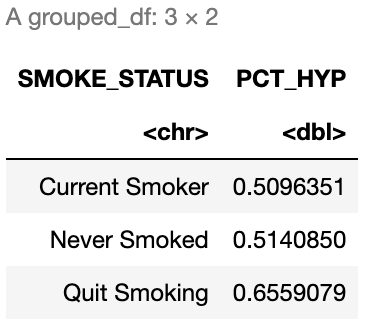
\includegraphics[width=2.08333in,height=\textheight]{book/images/5-practicequestion3answer.png}

}

\caption{\label{fig-pq3}Grouping and Summarizing Data.}

\end{figure}

\begin{Shaded}
\begin{Highlighting}[]
\CommentTok{\# Insert your solution here:}
\end{Highlighting}
\end{Shaded}

\hypertarget{exercises-3}{%
\section{Exercises}\label{exercises-3}}

The following exercises use the \texttt{covidcases} dataset from the
\textbf{HDSinRdata} package. Before completing the exercises, be sure to
read the documentation for this data (\texttt{?covidcases}).

\begin{Shaded}
\begin{Highlighting}[]
\FunctionTok{data}\NormalTok{(covidcases)}
\end{Highlighting}
\end{Shaded}

\begin{enumerate}
\def\labelenumi{\arabic{enumi}.}
\item
  Suppose we are interested in the distribution of weekly cases by
  state. First, create a new column in \texttt{covidcases} called
  \texttt{region} specifying whether each state is in the Northeast,
  Midwest, South, or West (you can either do this by hand using
  \href{https://en.wikipedia.org/wiki/List_of_regions_of_the_United_States}{this
  list} of which states are in which region or you can use
  \texttt{state.region} from the \textbf{datasets} package in R). Then,
  create a data frame summarizing the average and standard deviation of
  the weekly cases for the Northeast.
\item
  Now, create a data frame with the average and standard deviation
  summarized for each region rather than for just one selected region as
  in Question 1. Sort this data frame from highest to lowest average
  weekly cases. What other information would you need in order to more
  accurately compare these regions in terms of their average cases?
\item
  Find the ten counties in the Midwest with the lowest weekly deaths in
  week 15 of this data ignoring ties (use \texttt{slice\_min()} to find
  the argument needed for this). What do you notice about the minimum
  values? See the data documentation for why we observe these values.
\item
  Filter the data to between weeks 9 and 20 (around the start of the
  pandemic), get the total cases per county during that time frame, and
  then find the county in each state that had the highest number of
  total cases.
\end{enumerate}

\bookmarksetup{startatroot}

\hypertarget{sec-merging-reshaping}{%
\chapter{Merging and Reshaping Data}\label{sec-merging-reshaping}}

In this chapter, we continue to look at some of the ways to manipulate
data using the tidyverse packages. In particular, we will look at
reshaping and merging data frames in order to get the data in the format
we want. When reshaping data, we can convert between \emph{wide form}
(more columns, fewer rows) and \emph{long form} (fewer columns, more
rows). We can also use data pivots to put our data into what is called
\emph{tidy form}. Additionally, we will look at combining information
from multiple data frames into a single data frame. The key ideas when
merging data are to think about what the common information is between
the data frames and to consider which values we want to keep.

For this chapter, we will use three data sets. The first data set is
\texttt{covidcases}, which contains the weekly case and death counts by
county in the United States for 2020 (Guidotti and Ardia 2020; Guidotti
2022); the second data set is \texttt{mobility}, which contains daily
mobility estimates by state in 2020 (Warren and Skillman 2020); and the
third data set is \texttt{lockdowndates}, which contains the start and
end dates for statewide stay at home orders (Raifman et al. 2022). Take
a look at the first few rows of each data frame below and read the
documentation for the column descriptions.

\begin{Shaded}
\begin{Highlighting}[]
\FunctionTok{library}\NormalTok{(tidyverse)}
\FunctionTok{library}\NormalTok{(HDSinRdata)}
\FunctionTok{data}\NormalTok{(covidcases)}
\FunctionTok{data}\NormalTok{(lockdowndates)}
\FunctionTok{data}\NormalTok{(mobility)}
\end{Highlighting}
\end{Shaded}

\begin{Shaded}
\begin{Highlighting}[]
\FunctionTok{head}\NormalTok{(covidcases)}
\CommentTok{\#\textgreater{} \# A tibble: 6 x 5}
\CommentTok{\#\textgreater{} \# Groups:   state, county, week [6]}
\CommentTok{\#\textgreater{}   state   county   week weekly\_cases weekly\_deaths}
\CommentTok{\#\textgreater{}   \textless{}chr\textgreater{}   \textless{}chr\textgreater{}   \textless{}dbl\textgreater{}        \textless{}int\textgreater{}         \textless{}int\textgreater{}}
\CommentTok{\#\textgreater{} 1 Alabama Autauga    12            3             0}
\CommentTok{\#\textgreater{} 2 Alabama Autauga    13            3             0}
\CommentTok{\#\textgreater{} 3 Alabama Autauga    14            2             1}
\CommentTok{\#\textgreater{} 4 Alabama Autauga    15           11             1}
\CommentTok{\#\textgreater{} 5 Alabama Autauga    16            5             1}
\CommentTok{\#\textgreater{} \# i 1 more row}
\end{Highlighting}
\end{Shaded}

\begin{Shaded}
\begin{Highlighting}[]
\FunctionTok{head}\NormalTok{(mobility)}
\CommentTok{\#\textgreater{} \# A tibble: 6 x 5}
\CommentTok{\#\textgreater{} \# Groups:   state [1]}
\CommentTok{\#\textgreater{}   state   date       samples   m50 m50\_index}
\CommentTok{\#\textgreater{}   \textless{}chr\textgreater{}   \textless{}chr\textgreater{}        \textless{}int\textgreater{} \textless{}dbl\textgreater{}     \textless{}dbl\textgreater{}}
\CommentTok{\#\textgreater{} 1 Alabama 2020{-}03{-}01  267652  10.9      76.9}
\CommentTok{\#\textgreater{} 2 Alabama 2020{-}03{-}02  287264  14.3      98.6}
\CommentTok{\#\textgreater{} 3 Alabama 2020{-}03{-}03  292018  14.2      98.2}
\CommentTok{\#\textgreater{} 4 Alabama 2020{-}03{-}04  298704  13.1      89.7}
\CommentTok{\#\textgreater{} 5 Alabama 2020{-}03{-}05  288218  14.8     102. }
\CommentTok{\#\textgreater{} \# i 1 more row}
\end{Highlighting}
\end{Shaded}

\begin{Shaded}
\begin{Highlighting}[]
\FunctionTok{head}\NormalTok{(lockdowndates)}
\CommentTok{\#\textgreater{} \# A tibble: 6 x 3}
\CommentTok{\#\textgreater{}   State      Lockdown\_Start Lockdown\_End}
\CommentTok{\#\textgreater{}   \textless{}chr\textgreater{}      \textless{}chr\textgreater{}          \textless{}chr\textgreater{}       }
\CommentTok{\#\textgreater{} 1 Alabama    2020{-}04{-}04     2020{-}04{-}30  }
\CommentTok{\#\textgreater{} 2 Alaska     2020{-}03{-}28     2020{-}04{-}24  }
\CommentTok{\#\textgreater{} 3 Arizona    2020{-}03{-}31     2020{-}05{-}15  }
\CommentTok{\#\textgreater{} 4 Arkansas   None           None        }
\CommentTok{\#\textgreater{} 5 California 2020{-}03{-}19     2020{-}08{-}28  }
\CommentTok{\#\textgreater{} \# i 1 more row}
\end{Highlighting}
\end{Shaded}

Both the mobility and lockdown data frames contain date columns. Right
now, these columns in both data sets are of the class character, which
we can see in the printed output above. We can use the
\texttt{as.Date()} function to tell R to treat these columns as dates
instead of characters. When using this function, we need to specify the
date format as an argument so that R knows how to parse this text to a
date. Our format is given as \texttt{\%Y-\%M-\%D}, where the
\texttt{\%Y} stands for the full four-digit year, \texttt{\%M} is a
two-digit month (e.g.~January is coded ``01'' vs ``1''), and
\texttt{\%D} stands for the two-digit day (e.g.~the third day is coded
``03'' vs ``3''). Below, we convert the classes of these columns to
`Date'.

\begin{Shaded}
\begin{Highlighting}[]
\NormalTok{mobility}\SpecialCharTok{$}\NormalTok{date }\OtherTok{\textless{}{-}} \FunctionTok{as.Date}\NormalTok{(mobility}\SpecialCharTok{$}\NormalTok{date, }\AttributeTok{formula=}\StringTok{"\%Y{-}\%M{-}\%D"}\NormalTok{)}
\NormalTok{lockdowndates}\SpecialCharTok{$}\NormalTok{Lockdown\_Start }\OtherTok{\textless{}{-}} \FunctionTok{as.Date}\NormalTok{(lockdowndates}\SpecialCharTok{$}\NormalTok{Lockdown\_Start, }
                                        \AttributeTok{formula=}\StringTok{"\%Y{-}\%M{-}\%D"}\NormalTok{)}
\NormalTok{lockdowndates}\SpecialCharTok{$}\NormalTok{Lockdown\_End }\OtherTok{\textless{}{-}} \FunctionTok{as.Date}\NormalTok{(lockdowndates}\SpecialCharTok{$}\NormalTok{Lockdown\_End, }
                                      \AttributeTok{formula=}\StringTok{"\%Y{-}\%M{-}\%D"}\NormalTok{)}
\FunctionTok{class}\NormalTok{(mobility}\SpecialCharTok{$}\NormalTok{date)}
\CommentTok{\#\textgreater{} [1] "Date"}
\FunctionTok{class}\NormalTok{(lockdowndates}\SpecialCharTok{$}\NormalTok{Lockdown\_Start)}
\CommentTok{\#\textgreater{} [1] "Date"}
\FunctionTok{class}\NormalTok{(lockdowndates}\SpecialCharTok{$}\NormalTok{Lockdown\_End)}
\CommentTok{\#\textgreater{} [1] "Date"}
\end{Highlighting}
\end{Shaded}

After coding these columns as dates, we can access information such as
the day, month, year, or week from them. These functions are all
available in the \textbf{lubridate} package (Spinu, Grolemund, and
Wickham 2023), which is a package in the tidyverse that allows us to
manipulate dates.

\begin{Shaded}
\begin{Highlighting}[]
\FunctionTok{month}\NormalTok{(mobility}\SpecialCharTok{$}\NormalTok{date[}\DecValTok{1}\NormalTok{])}
\CommentTok{\#\textgreater{} [1] 3}
\FunctionTok{week}\NormalTok{(mobility}\SpecialCharTok{$}\NormalTok{date[}\DecValTok{1}\NormalTok{])}
\CommentTok{\#\textgreater{} [1] 9}
\end{Highlighting}
\end{Shaded}

Next, we add a date column to \texttt{covidcases}. In this case, we need
to use the week number to find the date. Luckily, we can add days,
months, weeks, or years to dates using the \textbf{lubridate} package.
January 1, 2020 was a Wednesday and is counted as the first week, so to
find the corresponding Sunday for each week, we add the recorded week
number minus one to December 29, 2019 (the last Sunday before 2020). We
show a simple example of adding one week to this date below before doing
this conversion for the entire column.

\begin{Shaded}
\begin{Highlighting}[]
\FunctionTok{as.Date}\NormalTok{(}\StringTok{"2019{-}12{-}29"}\NormalTok{)}\SpecialCharTok{+}\FunctionTok{weeks}\NormalTok{(}\DecValTok{1}\NormalTok{)}
\CommentTok{\#\textgreater{} [1] "2020{-}01{-}05"}
\end{Highlighting}
\end{Shaded}

\begin{Shaded}
\begin{Highlighting}[]
\NormalTok{covidcases}\SpecialCharTok{$}\NormalTok{date }\OtherTok{\textless{}{-}} \FunctionTok{as.Date}\NormalTok{(}\StringTok{"2019{-}12{-}29"}\NormalTok{)}\SpecialCharTok{+}\FunctionTok{weeks}\NormalTok{(covidcases}\SpecialCharTok{$}\NormalTok{week}\DecValTok{{-}1}\NormalTok{)}
\FunctionTok{head}\NormalTok{(covidcases)}
\CommentTok{\#\textgreater{} \# A tibble: 6 x 6}
\CommentTok{\#\textgreater{} \# Groups:   state, county, week [6]}
\CommentTok{\#\textgreater{}   state   county   week weekly\_cases weekly\_deaths date      }
\CommentTok{\#\textgreater{}   \textless{}chr\textgreater{}   \textless{}chr\textgreater{}   \textless{}dbl\textgreater{}        \textless{}int\textgreater{}         \textless{}int\textgreater{} \textless{}date\textgreater{}    }
\CommentTok{\#\textgreater{} 1 Alabama Autauga    12            3             0 2020{-}03{-}15}
\CommentTok{\#\textgreater{} 2 Alabama Autauga    13            3             0 2020{-}03{-}22}
\CommentTok{\#\textgreater{} 3 Alabama Autauga    14            2             1 2020{-}03{-}29}
\CommentTok{\#\textgreater{} 4 Alabama Autauga    15           11             1 2020{-}04{-}05}
\CommentTok{\#\textgreater{} 5 Alabama Autauga    16            5             1 2020{-}04{-}12}
\CommentTok{\#\textgreater{} \# i 1 more row}
\end{Highlighting}
\end{Shaded}

\hypertarget{tidy-data}{%
\section{Tidy Data}\label{tidy-data}}

The tidyverse is designed around interacting with \textbf{tidy data}
with the premise that using data in a tidy format can streamline our
analysis. Data is considered \textbf{tidy} if

\begin{itemize}
\item
  Each variable is associated with a single column.
\item
  Each observation is associated with a single row.
\item
  Each value has its own cell.
\end{itemize}

Take a look at the sample data below which stores information about the
maternal mortality rate for five countries over time (Roser and Ritchie,
n.d.). This data is \emph{not} tidy because the variable for maternity
mortality rate is associated with multiple columns. Every row should
correspond to one class observation.

\begin{Shaded}
\begin{Highlighting}[]
\NormalTok{mat\_mort1 }\OtherTok{\textless{}{-}} \FunctionTok{data.frame}\NormalTok{(}\AttributeTok{country =} \FunctionTok{c}\NormalTok{(}\StringTok{"Turkey"}\NormalTok{, }\StringTok{"United States"}\NormalTok{, }\StringTok{"Sweden"}\NormalTok{, }
                                    \StringTok{"Japan"}\NormalTok{),}
                       \AttributeTok{y2002 =} \FunctionTok{c}\NormalTok{(}\DecValTok{64}\NormalTok{, }\FloatTok{9.9}\NormalTok{, }\FloatTok{4.17}\NormalTok{, }\FloatTok{7.8}\NormalTok{),}
                       \AttributeTok{y2007 =} \FunctionTok{c}\NormalTok{(}\FloatTok{21.9}\NormalTok{, }\FloatTok{12.7}\NormalTok{, }\FloatTok{1.86}\NormalTok{, }\FloatTok{3.6}\NormalTok{),}
                       \AttributeTok{y2012 =} \FunctionTok{c}\NormalTok{(}\FloatTok{15.2}\NormalTok{, }\DecValTok{16}\NormalTok{, }\FloatTok{5.4}\NormalTok{, }\FloatTok{4.8}\NormalTok{))}
\FunctionTok{head}\NormalTok{(mat\_mort1)}
\CommentTok{\#\textgreater{}         country y2002 y2007 y2012}
\CommentTok{\#\textgreater{} 1        Turkey 64.00 21.90  15.2}
\CommentTok{\#\textgreater{} 2 United States  9.90 12.70  16.0}
\CommentTok{\#\textgreater{} 3        Sweden  4.17  1.86   5.4}
\CommentTok{\#\textgreater{} 4         Japan  7.80  3.60   4.8}
\end{Highlighting}
\end{Shaded}

However, we can make this data tidy by creating separate columns for
country, year, and maternity mortality rate as we demonstrate below. Now
every observation is associated with an individual row.

\begin{Shaded}
\begin{Highlighting}[]
\NormalTok{mat\_mort2 }\OtherTok{\textless{}{-}} \FunctionTok{data.frame}\NormalTok{(}
    \AttributeTok{country =} \FunctionTok{rep}\NormalTok{(}\FunctionTok{c}\NormalTok{(}\StringTok{"Turkey"}\NormalTok{, }\StringTok{"United States"}\NormalTok{, }\StringTok{"Sweden"}\NormalTok{, }\StringTok{"Japan"}\NormalTok{), }\DecValTok{3}\NormalTok{),}
    \AttributeTok{year =} \FunctionTok{c}\NormalTok{(}\FunctionTok{rep}\NormalTok{(}\DecValTok{2002}\NormalTok{, }\DecValTok{4}\NormalTok{), }\FunctionTok{rep}\NormalTok{(}\DecValTok{2007}\NormalTok{, }\DecValTok{4}\NormalTok{), }\FunctionTok{rep}\NormalTok{(}\DecValTok{2012}\NormalTok{, }\DecValTok{4}\NormalTok{)),}
    \AttributeTok{mat\_mort\_rate =} \FunctionTok{c}\NormalTok{(}\FloatTok{64.0}\NormalTok{, }\FloatTok{9.9}\NormalTok{, }\FloatTok{4.17}\NormalTok{, }\FloatTok{7.8}\NormalTok{, }\FloatTok{21.9}\NormalTok{, }\FloatTok{12.7}\NormalTok{, }\FloatTok{1.86}\NormalTok{, }\FloatTok{3.6}\NormalTok{, }
                      \FloatTok{15.2}\NormalTok{, }\DecValTok{16}\NormalTok{, }\FloatTok{5.4}\NormalTok{, }\FloatTok{4.8}\NormalTok{))}
\FunctionTok{head}\NormalTok{(mat\_mort2)}
\CommentTok{\#\textgreater{}         country year mat\_mort\_rate}
\CommentTok{\#\textgreater{} 1        Turkey 2002         64.00}
\CommentTok{\#\textgreater{} 2 United States 2002          9.90}
\CommentTok{\#\textgreater{} 3        Sweden 2002          4.17}
\CommentTok{\#\textgreater{} 4         Japan 2002          7.80}
\CommentTok{\#\textgreater{} 5        Turkey 2007         21.90}
\CommentTok{\#\textgreater{} 6 United States 2007         12.70}
\end{Highlighting}
\end{Shaded}

\hypertarget{reshaping-data}{%
\section{Reshaping Data}\label{reshaping-data}}

The mobility and covid case data are both already in tidy form - each
observation corresponds to a single row and every column is a single
variable. We might consider whether the lockdown dates should be
reformatted to be tidy. Another way to represent this data would be to
have each observation be the start or end of a stay at home order.

To reshape our data, we use the \texttt{pivot\_longer()} function to
change the data from what is called \textbf{wide form} to what is called
\textbf{long form}. This kind of pivot involves taking a subset of
columns that we will \emph{gather} into a single column while increasing
the number of rows in the data set. Before pivoting, we have to think
about which columns we are transforming. The image in
Figure~\ref{fig-pivot-long} shows a picture of some data on whether
students have completed a physical, hearing, or eye exam. The data is
presented in wide form on the left and long form on the right. To
transform wide data to long data, we have identified a subset of columns
\texttt{cols} that we want to transform (these \texttt{cols} are shown
in light purple on the left). The long form contains a new column
\texttt{names\_to} that contains the exam type and \texttt{values\_to}
that contains a binary variable indicating whether or not each exam was
completed.

\begin{figure}

{\centering 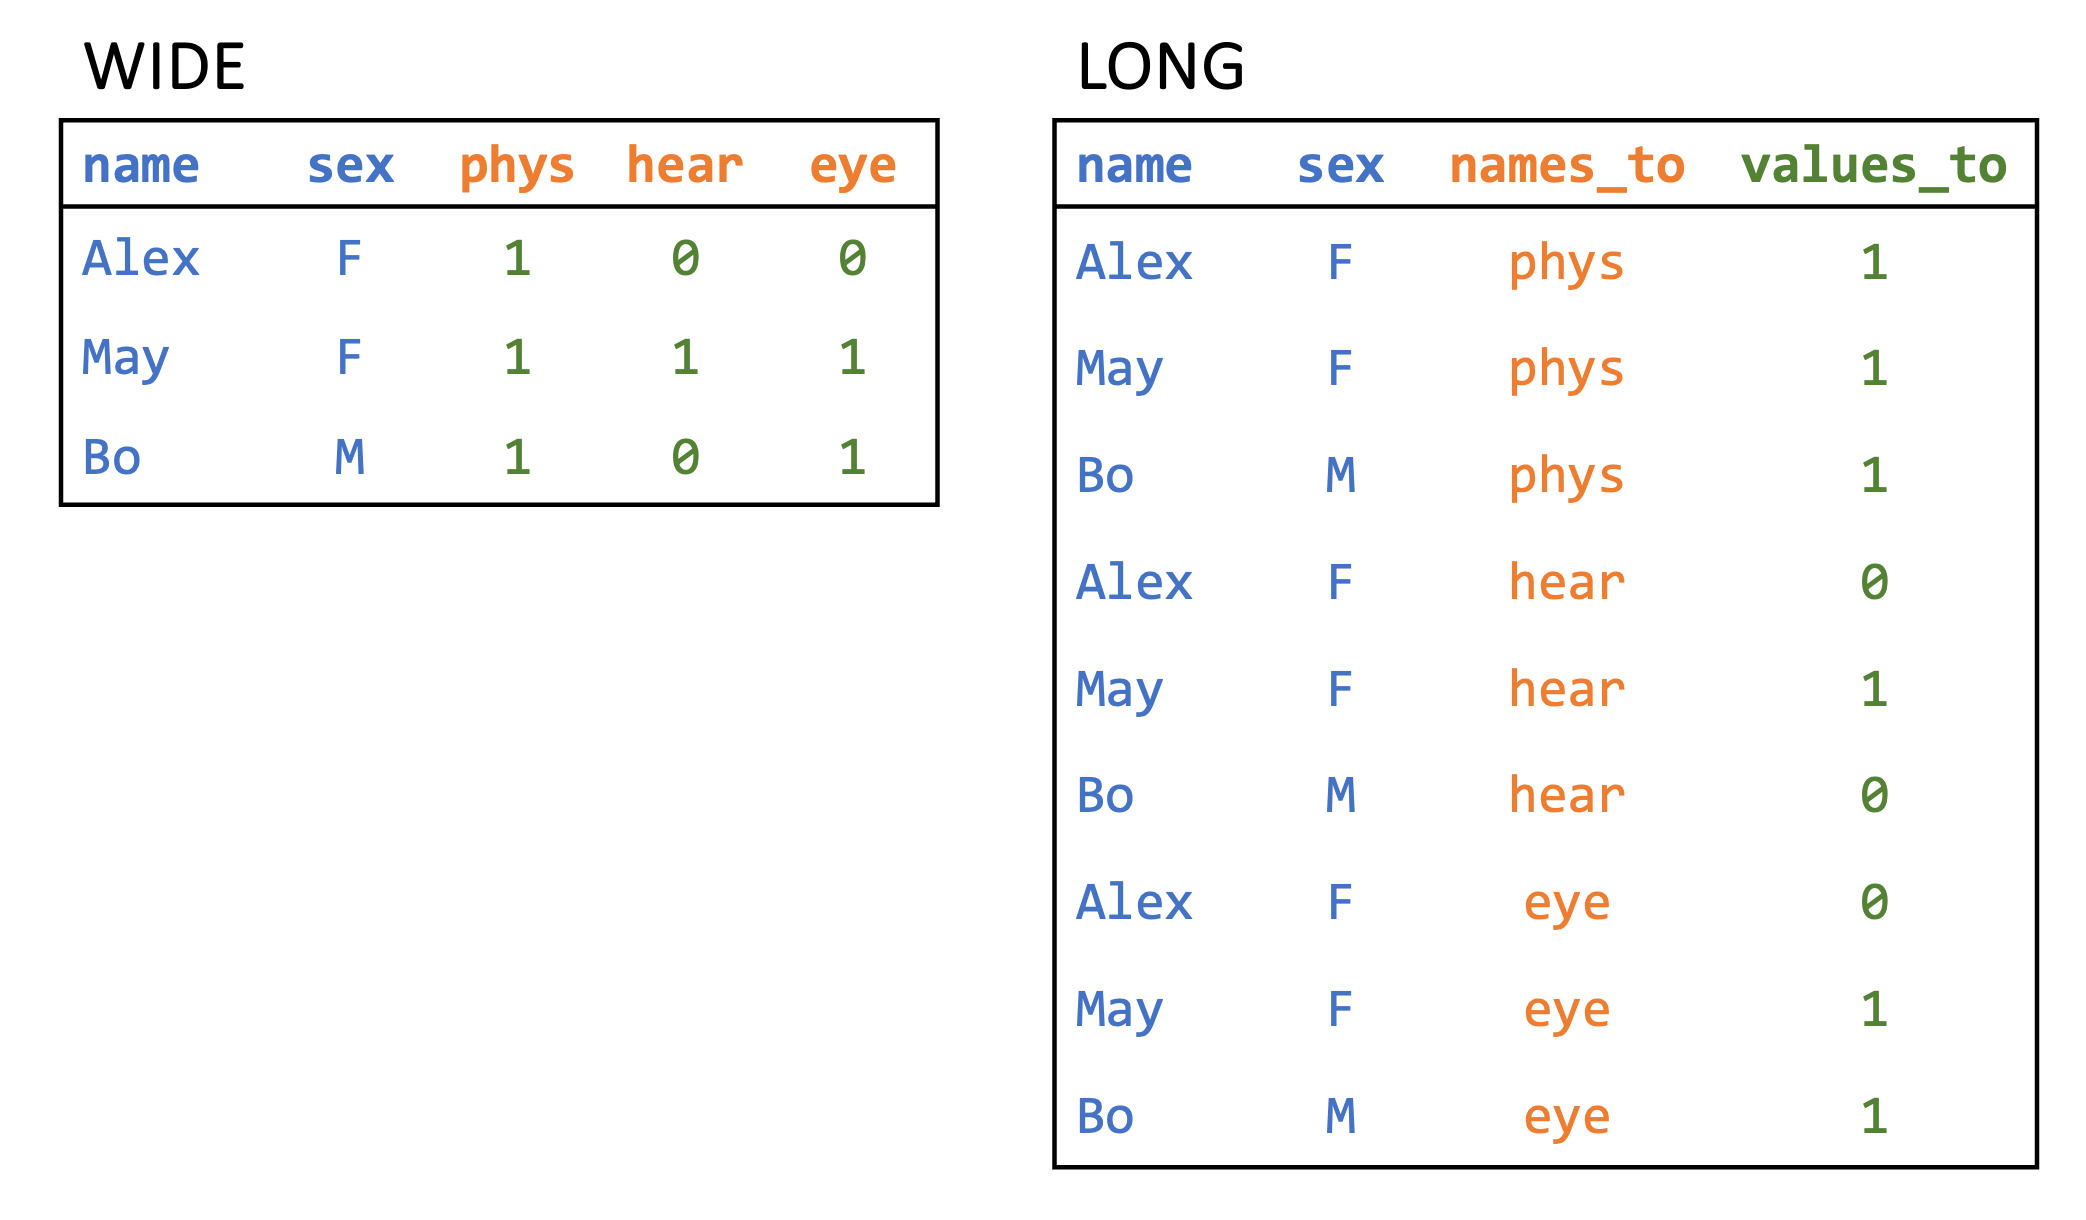
\includegraphics[width=4.16667in,height=\textheight]{book/images/6-pivot-long.png}

}

\caption{\label{fig-pivot-long}Pivoting Longer.}

\end{figure}

In our case, we want to take the lockdown start and end columns and
create two new columns: one column will indicate whether or not a date
represents the start or end of a lockdown, and the other will contain
the date itself. These are called the \emph{key} and \emph{value}
columns, respectively. The key column will get its values from the names
of the columns we are transforming (or the keys) whereas the value
column will get its values from the entries in those columns (or the
values).

The \texttt{pivot\_longer()} function takes in a data table, the columns
\texttt{cols} that we are pivoting to longer form, the column name
\texttt{names\_to} that will store the data from the previous column
names, and the column name \texttt{values\_to} for the column that will
store the information from the columns gathered. In our case, we will
name the first column \texttt{Lockdown\_Event} since it will contain
whether each date is the start or end of a lockdown, and we will name
the second column \texttt{Date}. Take a look at the result below.

\begin{Shaded}
\begin{Highlighting}[]
\NormalTok{lockdown\_long }\OtherTok{\textless{}{-}}\NormalTok{ lockdowndates }\SpecialCharTok{\%\textgreater{}\%}
  \FunctionTok{pivot\_longer}\NormalTok{(}\AttributeTok{cols=}\FunctionTok{c}\NormalTok{(}\StringTok{"Lockdown\_Start"}\NormalTok{, }\StringTok{"Lockdown\_End"}\NormalTok{), }
               \AttributeTok{names\_to=}\StringTok{"Lockdown\_Event"}\NormalTok{, }\AttributeTok{values\_to=}\StringTok{"Date"}\NormalTok{) }\SpecialCharTok{\%\textgreater{}\%}
  \FunctionTok{mutate}\NormalTok{(}\AttributeTok{Date =} \FunctionTok{as.Date}\NormalTok{(Date, }\AttributeTok{formula =}\StringTok{"\%Y{-}\%M{-}\%D"}\NormalTok{), }
         \AttributeTok{Lockdown\_Event =} \FunctionTok{ifelse}\NormalTok{(Lockdown\_Event}\SpecialCharTok{==}\StringTok{"Lockdown\_Start"}\NormalTok{, }
                                 \StringTok{"Start"}\NormalTok{, }\StringTok{"End"}\NormalTok{)) }\SpecialCharTok{\%\textgreater{}\%}
  \FunctionTok{na.omit}\NormalTok{()}
\FunctionTok{head}\NormalTok{(lockdown\_long)}
\CommentTok{\#\textgreater{} \# A tibble: 6 x 3}
\CommentTok{\#\textgreater{}   State   Lockdown\_Event Date      }
\CommentTok{\#\textgreater{}   \textless{}chr\textgreater{}   \textless{}chr\textgreater{}          \textless{}date\textgreater{}    }
\CommentTok{\#\textgreater{} 1 Alabama Start          2020{-}04{-}04}
\CommentTok{\#\textgreater{} 2 Alabama End            2020{-}04{-}30}
\CommentTok{\#\textgreater{} 3 Alaska  Start          2020{-}03{-}28}
\CommentTok{\#\textgreater{} 4 Alaska  End            2020{-}04{-}24}
\CommentTok{\#\textgreater{} 5 Arizona Start          2020{-}03{-}31}
\CommentTok{\#\textgreater{} \# i 1 more row}
\end{Highlighting}
\end{Shaded}

In R, we can also transform our data in the opposite direction (from
long form to wide form instead of from wide form to long form) using the
function \texttt{pivot\_wider()}. This function again first takes in a
data table but now we specify the arguments \texttt{names\_from} and
\texttt{values\_from}. The former indicates the column that R should get
the new column names from, and the latter indicates where the row values
should be taken from. For example, in order to pivot our lockdown data
back to wide form below, we specify that \texttt{names\_from} is the
lockdown event and \texttt{values\_from} is the date itself. Now we are
back to the same form as before!

\begin{Shaded}
\begin{Highlighting}[]
\NormalTok{lockdown\_wide }\OtherTok{\textless{}{-}} \FunctionTok{pivot\_wider}\NormalTok{(lockdown\_long, }\AttributeTok{names\_from=}\NormalTok{Lockdown\_Event, }
                             \AttributeTok{values\_from=}\NormalTok{Date)}
\FunctionTok{head}\NormalTok{(lockdown\_wide)}
\CommentTok{\#\textgreater{} \# A tibble: 6 x 3}
\CommentTok{\#\textgreater{}   State      Start      End       }
\CommentTok{\#\textgreater{}   \textless{}chr\textgreater{}      \textless{}date\textgreater{}     \textless{}date\textgreater{}    }
\CommentTok{\#\textgreater{} 1 Alabama    2020{-}04{-}04 2020{-}04{-}30}
\CommentTok{\#\textgreater{} 2 Alaska     2020{-}03{-}28 2020{-}04{-}24}
\CommentTok{\#\textgreater{} 3 Arizona    2020{-}03{-}31 2020{-}05{-}15}
\CommentTok{\#\textgreater{} 4 California 2020{-}03{-}19 2020{-}08{-}28}
\CommentTok{\#\textgreater{} 5 Colorado   2020{-}03{-}26 2020{-}04{-}26}
\CommentTok{\#\textgreater{} \# i 1 more row}
\end{Highlighting}
\end{Shaded}

Here's another example: suppose that I want to create a data frame where
the columns correspond to the number of cases for each state in New
England and the rows correspond to the numbered months. First, I need to
filter my data to New England and then summarize my data to find the
number of cases per month. I use the \texttt{month()} function to be
able to group by month and state. Additionally, you can see that I add
an \texttt{ungroup()} at the end. When we summarize on data grouped by
more than one variable, the summarized output will still be grouped. In
this case, the warning message states that the data is still grouped by
state.

\begin{Shaded}
\begin{Highlighting}[]
\NormalTok{ne\_cases }\OtherTok{\textless{}{-}}\NormalTok{ covidcases }\SpecialCharTok{\%\textgreater{}\%} 
  \FunctionTok{filter}\NormalTok{(state }\SpecialCharTok{\%in\%} \FunctionTok{c}\NormalTok{(}\StringTok{"Maine"}\NormalTok{, }\StringTok{"Vermont"}\NormalTok{, }\StringTok{"New Hampshire"}\NormalTok{, }\StringTok{"Connecticut"}\NormalTok{, }
                      \StringTok{"Rhode Island"}\NormalTok{, }\StringTok{"Massachusetts"}\NormalTok{)) }\SpecialCharTok{\%\textgreater{}\%}
  \FunctionTok{mutate}\NormalTok{(}\AttributeTok{month =} \FunctionTok{month}\NormalTok{(date)) }\SpecialCharTok{\%\textgreater{}\%}
  \FunctionTok{group\_by}\NormalTok{(state, month) }\SpecialCharTok{\%\textgreater{}\%}
  \FunctionTok{summarize}\NormalTok{(}\AttributeTok{total\_cases =} \FunctionTok{sum}\NormalTok{(weekly\_cases)) }\SpecialCharTok{\%\textgreater{}\%}
  \FunctionTok{ungroup}\NormalTok{()}
\FunctionTok{head}\NormalTok{(ne\_cases)}
\CommentTok{\#\textgreater{} \# A tibble: 6 x 3}
\CommentTok{\#\textgreater{}   state       month total\_cases}
\CommentTok{\#\textgreater{}   \textless{}chr\textgreater{}       \textless{}dbl\textgreater{}       \textless{}int\textgreater{}}
\CommentTok{\#\textgreater{} 1 Connecticut     3        6872}
\CommentTok{\#\textgreater{} 2 Connecticut     4       18575}
\CommentTok{\#\textgreater{} 3 Connecticut     5       11936}
\CommentTok{\#\textgreater{} 4 Connecticut     6        2619}
\CommentTok{\#\textgreater{} 5 Connecticut     7        2290}
\CommentTok{\#\textgreater{} \# i 1 more row}
\end{Highlighting}
\end{Shaded}

Now, I need to convert this data to wide format with a column for each
state, so my \texttt{names\_from} argument will be \texttt{state}.
Further, I want each row to have the case values for each state, so my
\texttt{values\_from} argument will be \texttt{total\_cases}. The format
of this data may not be tidy, but it allows me to quickly compare cases
across states.

\begin{Shaded}
\begin{Highlighting}[]
\FunctionTok{pivot\_wider}\NormalTok{(ne\_cases, }\AttributeTok{names\_from=}\NormalTok{state, }\AttributeTok{values\_from=}\NormalTok{total\_cases)}
\CommentTok{\#\textgreater{} \# A tibble: 7 x 7}
\CommentTok{\#\textgreater{}   month Connecticut Maine Massachusetts \textasciigrave{}New Hampshire\textasciigrave{} \textasciigrave{}Rhode Island\textasciigrave{} Vermont}
\CommentTok{\#\textgreater{}   \textless{}dbl\textgreater{}       \textless{}int\textgreater{} \textless{}int\textgreater{}         \textless{}int\textgreater{}           \textless{}int\textgreater{}          \textless{}int\textgreater{}   \textless{}int\textgreater{}}
\CommentTok{\#\textgreater{} 1     3        6872   434         13118             651            827     508}
\CommentTok{\#\textgreater{} 2     4       18575   725         47499            1649           6843     531}
\CommentTok{\#\textgreater{} 3     5       11936  1575         28798            2179          14653    1201}
\CommentTok{\#\textgreater{} 4     6        2619  1185          5545             751           1426     815}
\CommentTok{\#\textgreater{} 5     7        2290  1046          7621             827          65562     731}
\CommentTok{\#\textgreater{} \# i 2 more rows}
\end{Highlighting}
\end{Shaded}

\hypertarget{practice-question-11}{%
\subsection{Practice Question}\label{practice-question-11}}

Create a similar data frame as we did above but this time using the
\texttt{mobility} dataset. In other words, create a data frame where the
columns correspond to the average mobility for each state in New England
and the rows correspond to the numbered months. You should get a result
that looks like in Figure~\ref{fig-pq1}.

\begin{figure}

{\centering 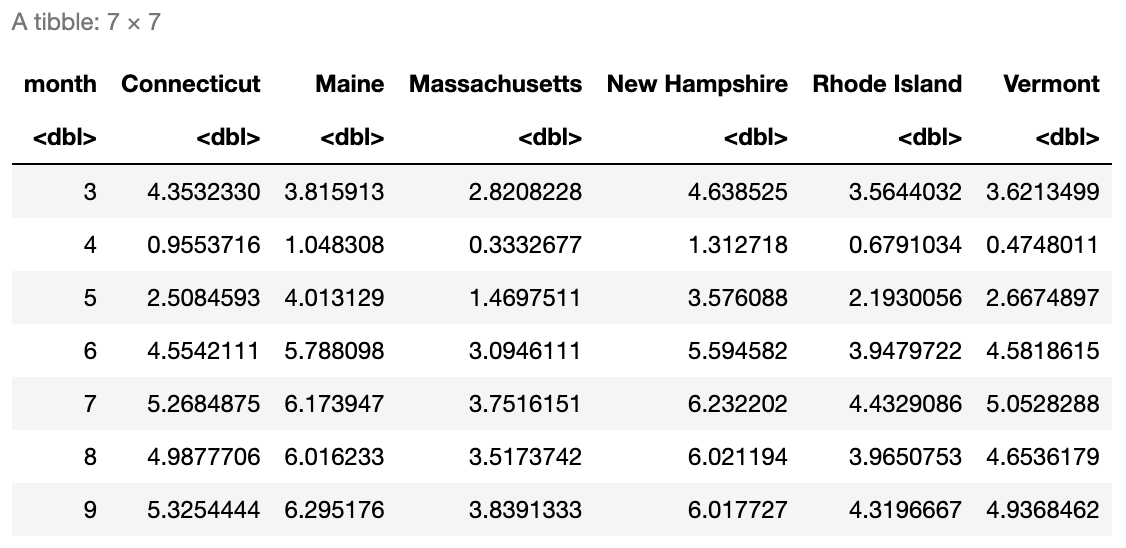
\includegraphics[width=3.47222in,height=\textheight]{book/images/6-practicequestion1answer.png}

}

\caption{\label{fig-pq1}Pivoting Mobility Data.}

\end{figure}

\begin{Shaded}
\begin{Highlighting}[]
\CommentTok{\# Insert your solution here:}
\end{Highlighting}
\end{Shaded}

The pivots above were relatively simple in that there was only one set
of values we were pivoting on (e.g.~the lockdown date, covid cases). The
\href{https://tidyr.tidyverse.org/articles/pivot.html}{\textbf{tidyr}
package} provides examples of more complex pivots that you might want to
apply to your data. In the video below, we demonstrate a pivot longer
when there is information in the column names, a pivot wider with
multiple value columns, and a pivot longer with many variables in the
columns.

\hypertarget{merging-data-with-joins}{%
\section{Merging Data with Joins}\label{merging-data-with-joins}}

Above, we saw how to manipulate our current data into new formats. Now,
we will see how we can combine multiple data sources. Merging two data
frames is called \emph{joining}, and the functions we will use to
perform this joining depends on how we want to match values between the
data frames. For example, below we join information about age and statin
use from \texttt{table1} and \texttt{table2} matching by name.

\begin{Shaded}
\begin{Highlighting}[]
\NormalTok{table1 }\OtherTok{\textless{}{-}} \FunctionTok{data.frame}\NormalTok{(}\AttributeTok{age =} \FunctionTok{c}\NormalTok{(}\DecValTok{14}\NormalTok{, }\DecValTok{26}\NormalTok{, }\DecValTok{32}\NormalTok{), }\AttributeTok{name =} \FunctionTok{c}\NormalTok{(}\StringTok{"Alice"}\NormalTok{, }\StringTok{"Bob"}\NormalTok{, }\StringTok{"Alice"}\NormalTok{))}
\NormalTok{table2 }\OtherTok{\textless{}{-}} \FunctionTok{data.frame}\NormalTok{(}\AttributeTok{name =} \FunctionTok{c}\NormalTok{(}\StringTok{"Carol"}\NormalTok{, }\StringTok{"Bob"}\NormalTok{), }\AttributeTok{statins =} \FunctionTok{c}\NormalTok{(}\ConstantTok{TRUE}\NormalTok{, }\ConstantTok{FALSE}\NormalTok{))}
\FunctionTok{full\_join}\NormalTok{(table1, table2, }\AttributeTok{by =} \StringTok{"name"}\NormalTok{)}
\CommentTok{\#\textgreater{}   age  name statins}
\CommentTok{\#\textgreater{} 1  14 Alice      NA}
\CommentTok{\#\textgreater{} 2  26   Bob   FALSE}
\CommentTok{\#\textgreater{} 3  32 Alice      NA}
\CommentTok{\#\textgreater{} 4  NA Carol    TRUE}
\end{Highlighting}
\end{Shaded}

The list below shows an overview of the different possible joins, and
the video talks through each join type. For each join type, we specify
two tables, \texttt{table1} and \texttt{table2}, and the \texttt{by}
argument, which specifies the columns used to match rows between tables.

\textbf{Types of Joins}:

\begin{itemize}
\tightlist
\item
  \texttt{left\_join(table1,\ table2,\ by)}: Joins each row of table1
  with all matches in table2.\\
\item
  \texttt{right\_join(table1,\ table2,\ by)}: Joins each row of table2
  with all matches in table1 (the opposite of a left join)\\
\item
  \texttt{inner\_join(table1,\ table2,\ by)}: Looks for all matches
  between rows in table1 and table2. Rows that do not find a match are
  dropped.\\
\item
  \texttt{full\_join(table1,\ table2,\ by)}: Keeps all rows from both
  tables and joins those that match. Rows that do not find a match will
  have NA values filled in.\\
\item
  \texttt{semi\_join(table1,\ table2,\ by)}: Keeps all rows in table1
  that have a match in table2 but does not join to any information from
  table2.\\
\item
  \texttt{anti\_join(table1,\ table2,\ by)}: Keeps all rows in table1
  that \emph{do not} have a match in table 2 but does not join to any
  information from table2. The opposite of a semi join.
\end{itemize}

We will first demonstrate a left join using the \texttt{left\_join()}
function. This function takes in two data tables (table1 and table 2)
and the columns to match rows by. In a left join, for every row of
table1, we look for all matching rows in table2 and add any columns not
used to do the matching. Thus, every row in table1 corresponds to at
least one entry in the resulting table but possibly more if there are
multiple matches. Below, we use a left join to add the lockdown
information to our \texttt{covidcases} data. In this case, the first
table will be \texttt{covidcases} and we will match by \texttt{state}.
Since the state column has a slightly different name in the two data
frames (``state'' in \texttt{covidcases} and ``State'' in
\texttt{lockdowndates}), we specify that \texttt{state} is equivalent to
\texttt{State} in the \texttt{by} argument.

\begin{Shaded}
\begin{Highlighting}[]
\NormalTok{covidcases\_full }\OtherTok{\textless{}{-}} \FunctionTok{left\_join}\NormalTok{(covidcases, lockdowndates, }\AttributeTok{by=}\FunctionTok{c}\NormalTok{(}\StringTok{"state"}\OtherTok{=}\StringTok{"State"}\NormalTok{))}
\FunctionTok{head}\NormalTok{(covidcases\_full)}
\CommentTok{\#\textgreater{} \# A tibble: 6 x 8}
\CommentTok{\#\textgreater{} \# Groups:   state, county, week [6]}
\CommentTok{\#\textgreater{}   state   county   week weekly\_cases weekly\_deaths date       Lockdown\_Start}
\CommentTok{\#\textgreater{}   \textless{}chr\textgreater{}   \textless{}chr\textgreater{}   \textless{}dbl\textgreater{}        \textless{}int\textgreater{}         \textless{}int\textgreater{} \textless{}date\textgreater{}     \textless{}date\textgreater{}        }
\CommentTok{\#\textgreater{} 1 Alabama Autauga    12            3             0 2020{-}03{-}15 2020{-}04{-}04    }
\CommentTok{\#\textgreater{} 2 Alabama Autauga    13            3             0 2020{-}03{-}22 2020{-}04{-}04    }
\CommentTok{\#\textgreater{} 3 Alabama Autauga    14            2             1 2020{-}03{-}29 2020{-}04{-}04    }
\CommentTok{\#\textgreater{} 4 Alabama Autauga    15           11             1 2020{-}04{-}05 2020{-}04{-}04    }
\CommentTok{\#\textgreater{} 5 Alabama Autauga    16            5             1 2020{-}04{-}12 2020{-}04{-}04    }
\CommentTok{\#\textgreater{} \# i 1 more row}
\CommentTok{\#\textgreater{} \# i 1 more variable: Lockdown\_End \textless{}date\textgreater{}}
\end{Highlighting}
\end{Shaded}

These two new columns will allow us to determine whether the start of
each recorded week was during a lockdown. We use the \texttt{between}
function to create a new column \texttt{lockdown} before dropping the
two date columns. We can check that this column worked as expected by
choosing a single county to look at.

\begin{Shaded}
\begin{Highlighting}[]
\NormalTok{covidcases\_full }\OtherTok{\textless{}{-}}\NormalTok{ covidcases\_full }\SpecialCharTok{\%\textgreater{}\%}
  \FunctionTok{mutate}\NormalTok{(}\AttributeTok{lockdown =} \FunctionTok{between}\NormalTok{(date, Lockdown\_Start, Lockdown\_End)) }\SpecialCharTok{\%\textgreater{}\%}
  \FunctionTok{select}\NormalTok{(}\SpecialCharTok{{-}}\FunctionTok{c}\NormalTok{(Lockdown\_Start, Lockdown\_End)) }
\NormalTok{covidcases\_full }\SpecialCharTok{\%\textgreater{}\%}
  \FunctionTok{filter}\NormalTok{(state }\SpecialCharTok{==} \StringTok{"Alabama"}\NormalTok{, county }\SpecialCharTok{==} \StringTok{"Jefferson"}\NormalTok{, }
\NormalTok{         date }\SpecialCharTok{\textless{}=} \FunctionTok{as.Date}\NormalTok{(}\StringTok{"2020{-}05{-}10"}\NormalTok{))}
\CommentTok{\#\textgreater{} \# A tibble: 10 x 7}
\CommentTok{\#\textgreater{} \# Groups:   state, county, week [10]}
\CommentTok{\#\textgreater{}   state   county     week weekly\_cases weekly\_deaths date       lockdown}
\CommentTok{\#\textgreater{}   \textless{}chr\textgreater{}   \textless{}chr\textgreater{}     \textless{}dbl\textgreater{}        \textless{}int\textgreater{}         \textless{}int\textgreater{} \textless{}date\textgreater{}     \textless{}lgl\textgreater{}   }
\CommentTok{\#\textgreater{} 1 Alabama Jefferson    11           19             0 2020{-}03{-}08 FALSE   }
\CommentTok{\#\textgreater{} 2 Alabama Jefferson    12           66             0 2020{-}03{-}15 FALSE   }
\CommentTok{\#\textgreater{} 3 Alabama Jefferson    13          153             0 2020{-}03{-}22 FALSE   }
\CommentTok{\#\textgreater{} 4 Alabama Jefferson    14          156             8 2020{-}03{-}29 FALSE   }
\CommentTok{\#\textgreater{} 5 Alabama Jefferson    15          128             2 2020{-}04{-}05 TRUE    }
\CommentTok{\#\textgreater{} \# i 5 more rows}
\end{Highlighting}
\end{Shaded}

We now want to add in the mobility data. In the join above, we wanted to
keep any observation in \texttt{covidcases} regardless if it was in the
\texttt{lockdowndates} data frame. Therefore, we used a left join. In
this case, we will only want to keep observations that have mobility
date for that state on each date. This indicates that we want to use an
\emph{inner join}. The function \texttt{inner\_join()} takes in two data
tables (table1 and table2) and the columns to match rows by. The
function only keeps rows in table1 that match to a row in table2. Again,
those columns in table2 not used to match with table1 are added to the
resulting outcome. In this case, we match by both state and date.

\begin{Shaded}
\begin{Highlighting}[]
\NormalTok{covidcases\_full }\OtherTok{\textless{}{-}} \FunctionTok{inner\_join}\NormalTok{(covidcases\_full, mobility, }
                              \AttributeTok{by =} \FunctionTok{c}\NormalTok{(}\StringTok{"state"}\NormalTok{, }\StringTok{"date"}\NormalTok{)) }\SpecialCharTok{\%\textgreater{}\%}
  \FunctionTok{select}\NormalTok{(}\SpecialCharTok{{-}}\FunctionTok{c}\NormalTok{(samples, m50\_index))}
\FunctionTok{head}\NormalTok{(covidcases\_full)}
\CommentTok{\#\textgreater{} \# A tibble: 6 x 8}
\CommentTok{\#\textgreater{} \# Groups:   state, county, week [6]}
\CommentTok{\#\textgreater{}   state   county   week weekly\_cases weekly\_deaths date       lockdown   m50}
\CommentTok{\#\textgreater{}   \textless{}chr\textgreater{}   \textless{}chr\textgreater{}   \textless{}dbl\textgreater{}        \textless{}int\textgreater{}         \textless{}int\textgreater{} \textless{}date\textgreater{}     \textless{}lgl\textgreater{}    \textless{}dbl\textgreater{}}
\CommentTok{\#\textgreater{} 1 Alabama Autauga    12            3             0 2020{-}03{-}15 FALSE    8.77 }
\CommentTok{\#\textgreater{} 2 Alabama Autauga    13            3             0 2020{-}03{-}22 FALSE    4.73 }
\CommentTok{\#\textgreater{} 3 Alabama Autauga    14            2             1 2020{-}03{-}29 FALSE    4.43 }
\CommentTok{\#\textgreater{} 4 Alabama Autauga    15           11             1 2020{-}04{-}05 TRUE     2.27 }
\CommentTok{\#\textgreater{} 5 Alabama Autauga    16            5             1 2020{-}04{-}12 TRUE     0.759}
\CommentTok{\#\textgreater{} \# i 1 more row}
\end{Highlighting}
\end{Shaded}

\hypertarget{practice-question-12}{%
\subsection{Practice Question}\label{practice-question-12}}

Look at the two data frames, \texttt{df\_A} and \texttt{df\_B}, created
in the below code. What kind of join would produce the data frame in
Figure~\ref{fig-pq2}? Perform this join yourself.

\begin{figure}

{\centering 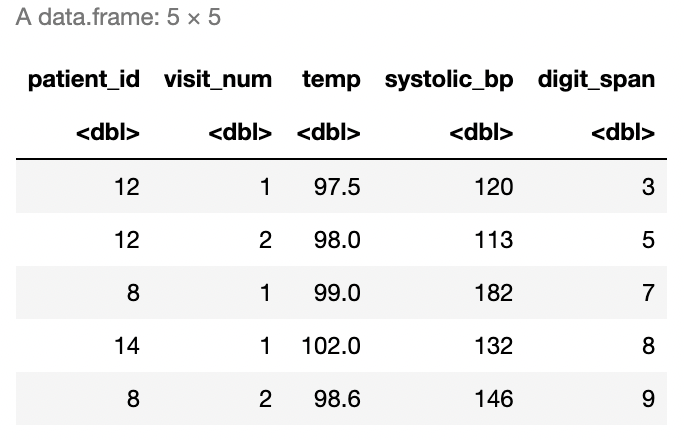
\includegraphics[width=2.08333in,height=\textheight]{book/images/6-practicequestion2answer.png}

}

\caption{\label{fig-pq2}Joining Data.}

\end{figure}

\begin{Shaded}
\begin{Highlighting}[]
\NormalTok{df\_A }\OtherTok{\textless{}{-}} \FunctionTok{data.frame}\NormalTok{(}\AttributeTok{patient\_id =} \FunctionTok{c}\NormalTok{(}\DecValTok{12}\NormalTok{, }\DecValTok{9}\NormalTok{, }\DecValTok{12}\NormalTok{, }\DecValTok{8}\NormalTok{, }\DecValTok{14}\NormalTok{, }\DecValTok{8}\NormalTok{), }
                  \AttributeTok{visit\_num =} \FunctionTok{c}\NormalTok{(}\DecValTok{1}\NormalTok{, }\DecValTok{1}\NormalTok{, }\DecValTok{2}\NormalTok{, }\DecValTok{1}\NormalTok{, }\DecValTok{1}\NormalTok{, }\DecValTok{2}\NormalTok{), }
                  \AttributeTok{temp =} \FunctionTok{c}\NormalTok{(}\FloatTok{97.5}\NormalTok{, }\DecValTok{96}\NormalTok{, }\DecValTok{98}\NormalTok{, }\DecValTok{99}\NormalTok{, }\DecValTok{102}\NormalTok{, }\FloatTok{98.6}\NormalTok{), }
                  \AttributeTok{systolic\_bp =} \FunctionTok{c}\NormalTok{(}\DecValTok{120}\NormalTok{, }\DecValTok{138}\NormalTok{, }\DecValTok{113}\NormalTok{, }\DecValTok{182}\NormalTok{, }\DecValTok{132}\NormalTok{, }\DecValTok{146}\NormalTok{))}
\NormalTok{df\_A}
\CommentTok{\#\textgreater{}   patient\_id visit\_num  temp systolic\_bp}
\CommentTok{\#\textgreater{} 1         12         1  97.5         120}
\CommentTok{\#\textgreater{} 2          9         1  96.0         138}
\CommentTok{\#\textgreater{} 3         12         2  98.0         113}
\CommentTok{\#\textgreater{} 4          8         1  99.0         182}
\CommentTok{\#\textgreater{} 5         14         1 102.0         132}
\CommentTok{\#\textgreater{} 6          8         2  98.6         146}
\NormalTok{df\_B }\OtherTok{\textless{}{-}} \FunctionTok{data.frame}\NormalTok{(}\AttributeTok{patient\_id =} \FunctionTok{c}\NormalTok{(}\DecValTok{12}\NormalTok{, }\DecValTok{12}\NormalTok{, }\DecValTok{12}\NormalTok{, }\DecValTok{8}\NormalTok{, }\DecValTok{8}\NormalTok{, }\DecValTok{8}\NormalTok{, }\DecValTok{14}\NormalTok{, }\DecValTok{14}\NormalTok{), }
                   \AttributeTok{visit\_num =} \FunctionTok{c}\NormalTok{(}\DecValTok{1}\NormalTok{, }\DecValTok{2}\NormalTok{, }\DecValTok{3}\NormalTok{, }\DecValTok{1}\NormalTok{, }\DecValTok{2}\NormalTok{, }\DecValTok{3}\NormalTok{, }\DecValTok{1}\NormalTok{, }\DecValTok{2}\NormalTok{),}
                   \AttributeTok{digit\_span =} \FunctionTok{c}\NormalTok{(}\DecValTok{3}\NormalTok{, }\DecValTok{5}\NormalTok{, }\DecValTok{7}\NormalTok{, }\DecValTok{7}\NormalTok{, }\DecValTok{9}\NormalTok{, }\DecValTok{5}\NormalTok{, }\DecValTok{8}\NormalTok{, }\DecValTok{7}\NormalTok{))}
\NormalTok{df\_B}
\CommentTok{\#\textgreater{}   patient\_id visit\_num digit\_span}
\CommentTok{\#\textgreater{} 1         12         1          3}
\CommentTok{\#\textgreater{} 2         12         2          5}
\CommentTok{\#\textgreater{} 3         12         3          7}
\CommentTok{\#\textgreater{} 4          8         1          7}
\CommentTok{\#\textgreater{} 5          8         2          9}
\CommentTok{\#\textgreater{} 6          8         3          5}
\CommentTok{\#\textgreater{} 7         14         1          8}
\CommentTok{\#\textgreater{} 8         14         2          7}
\end{Highlighting}
\end{Shaded}

\begin{Shaded}
\begin{Highlighting}[]
\CommentTok{\# Insert your solution here:}
\end{Highlighting}
\end{Shaded}

\hypertarget{exercises-4}{%
\section{Exercises}\label{exercises-4}}

\begin{enumerate}
\def\labelenumi{\arabic{enumi}.}
\item
  Take a look at the code below - what is wrong with it? Hint: think
  about what causes the warning message.

\begin{Shaded}
\begin{Highlighting}[]
\NormalTok{visit\_info }\OtherTok{\textless{}{-}} \FunctionTok{data.frame}\NormalTok{(}
  \AttributeTok{name.f =} \FunctionTok{c}\NormalTok{(}\StringTok{"Phillip"}\NormalTok{, }\StringTok{"Phillip"}\NormalTok{, }\StringTok{"Phillip"}\NormalTok{, }\StringTok{"Jessica"}\NormalTok{, }\StringTok{"Jessica"}\NormalTok{),}
  \AttributeTok{name.l =} \FunctionTok{c}\NormalTok{(}\StringTok{"Johnson"}\NormalTok{, }\StringTok{"Johnson"}\NormalTok{, }\StringTok{"Richards"}\NormalTok{, }\StringTok{"Smith"}\NormalTok{, }\StringTok{"Abrams"}\NormalTok{),}
  \AttributeTok{measure =} \FunctionTok{c}\NormalTok{(}\StringTok{"height"}\NormalTok{, }\StringTok{"age"}\NormalTok{, }\StringTok{"age"}\NormalTok{, }\StringTok{"age"}\NormalTok{, }\StringTok{"height"}\NormalTok{),}
  \AttributeTok{measurement =} \FunctionTok{c}\NormalTok{(}\DecValTok{45}\NormalTok{, }\DecValTok{186}\NormalTok{, }\DecValTok{50}\NormalTok{, }\DecValTok{37}\NormalTok{, }\DecValTok{156}\NormalTok{)}
\NormalTok{)}

\NormalTok{contact\_info }\OtherTok{\textless{}{-}} \FunctionTok{data.frame}\NormalTok{(}
\AttributeTok{first\_name =} \FunctionTok{c}\NormalTok{(}\StringTok{"Phillip"}\NormalTok{, }\StringTok{"Phillip"}\NormalTok{, }\StringTok{"Jessica"}\NormalTok{, }\StringTok{"Margaret"}\NormalTok{),}
\AttributeTok{last\_name =} \FunctionTok{c}\NormalTok{(}\StringTok{"Richards"}\NormalTok{, }\StringTok{"Johnson"}\NormalTok{, }\StringTok{"Smith"}\NormalTok{, }\StringTok{"Reynolds"}\NormalTok{),}
\AttributeTok{email =} \FunctionTok{c}\NormalTok{(}\StringTok{"pr@aol.com"}\NormalTok{, }\StringTok{"phillipj@gmail.com"}\NormalTok{, }\StringTok{"jesssmith@brown.edu"}\NormalTok{, }
      \StringTok{"marg@hotmail.com"}\NormalTok{)}
\NormalTok{)}

\FunctionTok{left\_join}\NormalTok{(visit\_info, contact\_info, }\AttributeTok{by =} \FunctionTok{c}\NormalTok{(}\StringTok{"name.f"} \OtherTok{=} \StringTok{"first\_name"}\NormalTok{))}
\CommentTok{\#\textgreater{} Warning in left\_join(visit\_info, contact\_info, by = c(name.f = "first\_name")): Detected an unexpected many{-}to{-}many relationship between \textasciigrave{}x\textasciigrave{} and \textasciigrave{}y\textasciigrave{}.}
\CommentTok{\#\textgreater{} i Row 1 of \textasciigrave{}x\textasciigrave{} matches multiple rows in \textasciigrave{}y\textasciigrave{}.}
\CommentTok{\#\textgreater{} i Row 1 of \textasciigrave{}y\textasciigrave{} matches multiple rows in \textasciigrave{}x\textasciigrave{}.}
\CommentTok{\#\textgreater{} i If a many{-}to{-}many relationship is expected, set \textasciigrave{}relationship =}
\CommentTok{\#\textgreater{}   "many{-}to{-}many"\textasciigrave{} to silence this warning.}
\CommentTok{\#\textgreater{}    name.f   name.l measure measurement last\_name               email}
\CommentTok{\#\textgreater{} 1 Phillip  Johnson  height          45  Richards          pr@aol.com}
\CommentTok{\#\textgreater{} 2 Phillip  Johnson  height          45   Johnson  phillipj@gmail.com}
\CommentTok{\#\textgreater{} 3 Phillip  Johnson     age         186  Richards          pr@aol.com}
\CommentTok{\#\textgreater{} 4 Phillip  Johnson     age         186   Johnson  phillipj@gmail.com}
\CommentTok{\#\textgreater{} 5 Phillip Richards     age          50  Richards          pr@aol.com}
\CommentTok{\#\textgreater{} 6 Phillip Richards     age          50   Johnson  phillipj@gmail.com}
\CommentTok{\#\textgreater{} 7 Jessica    Smith     age          37     Smith jesssmith@brown.edu}
\CommentTok{\#\textgreater{} 8 Jessica   Abrams  height         156     Smith jesssmith@brown.edu}
\end{Highlighting}
\end{Shaded}
\item
  First, use the \texttt{covidcases} data to create a new data frame
  called \texttt{sub\_cases} containing the total number of cases by
  month for the states of California, Michigan, Connecticut, Rhode
  Island, Ohio, New York, and Massachusetts. Then, manipulate the
  \texttt{mobility} data to calculate the average \texttt{m50} mobility
  measure for each month. Finally, merge these two data sets using an
  appropriate joining function.
\item
  Convert the \texttt{sub\_cases} data frame from the previous exercise
  to wide format so that each row displays the cases in each state for a
  single month. Then, add on the average m50 overall for each month as
  an additional column using a join function.
\end{enumerate}

\bookmarksetup{startatroot}

\hypertarget{sec-ggplot2}{%
\chapter{Visualization with ggplot2}\label{sec-ggplot2}}

The package \textbf{ggplot2} is another useful package in the tidyverse
that allows statisticians to use visualizations to communicate key
findings and results in a compelling format. We will first learn about
the three main components in a ggplot object and then expand on that
format by learning more about the different layers we can use to create
various plots. As with the tidyverse functions, there are quite a few
functions to cover, and the functions build on each other.

The three packages we will use in this chapter are \textbf{tidyverse},
\textbf{HDSinRdata}, and \textbf{patchwork} (Pedersen 2022), the last of
which is a nice package for combining multiple plots together into a
single figure. We will use the data from the Pittsburgh pain clinic
(Alter et al. 2021) introduced in Chapter~\ref{sec-data-files} to create
our visuals. You can refresh your memory about this data by reading the
data documentation. For the purposes of this chapter, we take a sample
of 5,000 patients that are complete cases at baseline to reduce the
computation time to display each plot. You can ignore how the code used
to find this sample works.

\begin{Shaded}
\begin{Highlighting}[]
\FunctionTok{library}\NormalTok{(tidyverse)}
\FunctionTok{library}\NormalTok{(HDSinRdata)}
\FunctionTok{library}\NormalTok{(patchwork)}
\FunctionTok{data}\NormalTok{(pain)}

\CommentTok{\# sampling data}
\FunctionTok{set.seed}\NormalTok{(}\DecValTok{5}\NormalTok{)}
\NormalTok{pain\_df\_sub }\OtherTok{\textless{}{-}} \FunctionTok{subset}\NormalTok{(pain, }\AttributeTok{select=}\SpecialCharTok{{-}}\FunctionTok{c}\NormalTok{(PAIN\_INTENSITY\_AVERAGE.FOLLOW\_UP))}
\NormalTok{pain\_df }\OtherTok{\textless{}{-}}\NormalTok{ pain[}\FunctionTok{complete.cases}\NormalTok{(pain\_df\_sub),]}
\NormalTok{pain\_df }\OtherTok{\textless{}{-}}\NormalTok{ pain\_df[}\FunctionTok{sample}\NormalTok{(}\DecValTok{1}\SpecialCharTok{:}\FunctionTok{nrow}\NormalTok{(pain\_df), }\DecValTok{5000}\NormalTok{, }\AttributeTok{replace=}\ConstantTok{FALSE}\NormalTok{),] }
\end{Highlighting}
\end{Shaded}

\hypertarget{intro-to-ggplot}{%
\section{Intro to ggplot}\label{intro-to-ggplot}}

We'll begin by demonstrating how to create a scatter plot in
\texttt{ggplot2} to introduce the three key elements of a
\texttt{ggplot2} object. Specifically, we will create a scatter plot of
a patient's depression vs.~anxiety score. To start a graph, we can use
the \texttt{ggplot()} function to create a \texttt{ggplot} object as
below. Note that this brings up a gray box - this will be the base that
we will build up from.

\begin{Shaded}
\begin{Highlighting}[]
\FunctionTok{ggplot}\NormalTok{()}
\end{Highlighting}
\end{Shaded}

\begin{figure}[H]

{\centering 
\includegraphics[width=1\textwidth,height=\textheight]{book/7_visualization_ggplot_files/figure-pdf/unnamed-chunk-2-1.pdf}

}

\end{figure}

Now we can start adding layers to our \texttt{ggplot} object. One type
of layer is a \textbf{geom}, which creates a geometric object. Below, we
use the \texttt{geom\_point()} function to add a scatter plot layer. For
this function, we first need to specify which data we want to use, and
then we need to tell R how to use that data to create the scatter plot
using the \texttt{aes()} function, which creates an \textbf{aesthetic}.
For a scatter plot, we need to at least specify the x-axis and y-axis in
the aesthetic. Both the data and the aesthetic can either be specified
in our initial \texttt{ggplot()} function, which will pass this
information to all future layers, or in the \texttt{geom\_point()}
function itself. Below, we specify the aesthetic in the geom function
but also include two alternative ways to code the same image that are
commented out. The resulting plot shows a fairly linear relationship
between anxiety and depression.

\begin{Shaded}
\begin{Highlighting}[]
\FunctionTok{ggplot}\NormalTok{(pain\_df) }\SpecialCharTok{+} \FunctionTok{geom\_point}\NormalTok{(}\FunctionTok{aes}\NormalTok{(}\AttributeTok{x=}\NormalTok{PROMIS\_ANXIETY, }\AttributeTok{y =}\NormalTok{ PROMIS\_DEPRESSION))}
\end{Highlighting}
\end{Shaded}

\begin{figure}[H]

{\centering 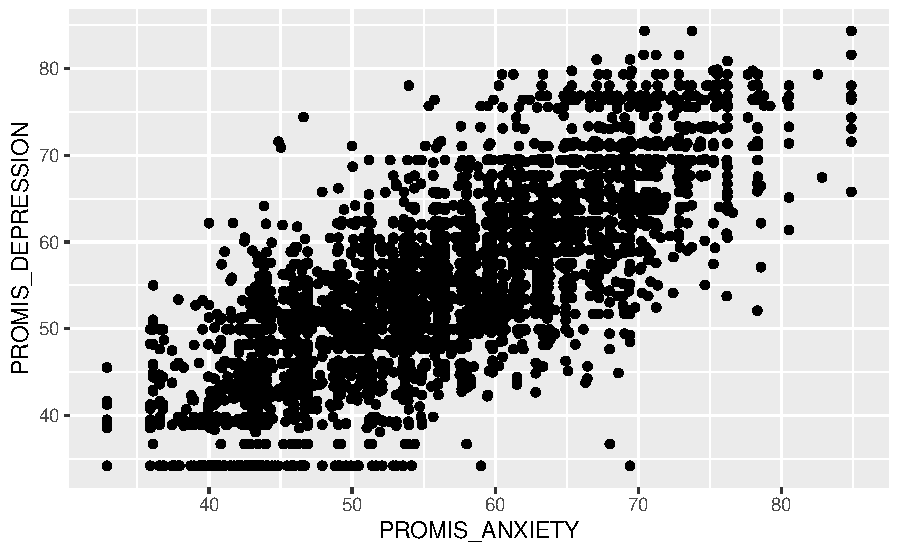
\includegraphics[width=1\textwidth,height=\textheight]{book/7_visualization_ggplot_files/figure-pdf/unnamed-chunk-3-1.pdf}

}

\end{figure}

\begin{Shaded}
\begin{Highlighting}[]
\CommentTok{\# Alternative 1:}
\FunctionTok{ggplot}\NormalTok{(pain\_df, }\FunctionTok{aes}\NormalTok{(}\AttributeTok{x=}\NormalTok{PROMIS\_ANXIETY, }\AttributeTok{y =}\NormalTok{ PROMIS\_DEPRESSION)) }\SpecialCharTok{+} \FunctionTok{geom\_point}\NormalTok{()}
\CommentTok{\# Alternative 2:}
\FunctionTok{ggplot}\NormalTok{() }\SpecialCharTok{+} \FunctionTok{geom\_point}\NormalTok{(}\AttributeTok{data =}\NormalTok{ pain\_df, }\FunctionTok{aes}\NormalTok{(}\AttributeTok{x=}\NormalTok{PROMIS\_ANXIETY, }
                                          \AttributeTok{y =}\NormalTok{ PROMIS\_DEPRESSION))}
\end{Highlighting}
\end{Shaded}

If we want to improve our plot, we may want to add different labels and
a title. To do so, we use the \texttt{labs()} function to add a layer in
which we can specify all labels. Additionally, I have passed more
information to the geometry layer by changing the color, size, and shape
of the points. These things are specified outside of the \texttt{aes()}
function since they do not come from the data - every point has the same
color, size, and shape in this example.

\begin{Shaded}
\begin{Highlighting}[]
\FunctionTok{ggplot}\NormalTok{(pain\_df)}\SpecialCharTok{+}
  \FunctionTok{geom\_point}\NormalTok{(}\FunctionTok{aes}\NormalTok{(}\AttributeTok{x=}\NormalTok{PROMIS\_ANXIETY, }\AttributeTok{y =}\NormalTok{ PROMIS\_DEPRESSION), }
             \AttributeTok{color=}\StringTok{"blue"}\NormalTok{, }\AttributeTok{size=}\DecValTok{2}\NormalTok{, }\AttributeTok{shape=}\DecValTok{5}\NormalTok{) }\SpecialCharTok{+} 
  \FunctionTok{labs}\NormalTok{(}\AttributeTok{x=}\StringTok{"PROMIS Anxiety Score"}\NormalTok{, }\AttributeTok{ylab=}\StringTok{"PROMIS Depression Score"}\NormalTok{, }
       \AttributeTok{title =} \StringTok{"Depression vs Anxiety Scores"}\NormalTok{)}
\end{Highlighting}
\end{Shaded}

\begin{figure}[H]

{\centering 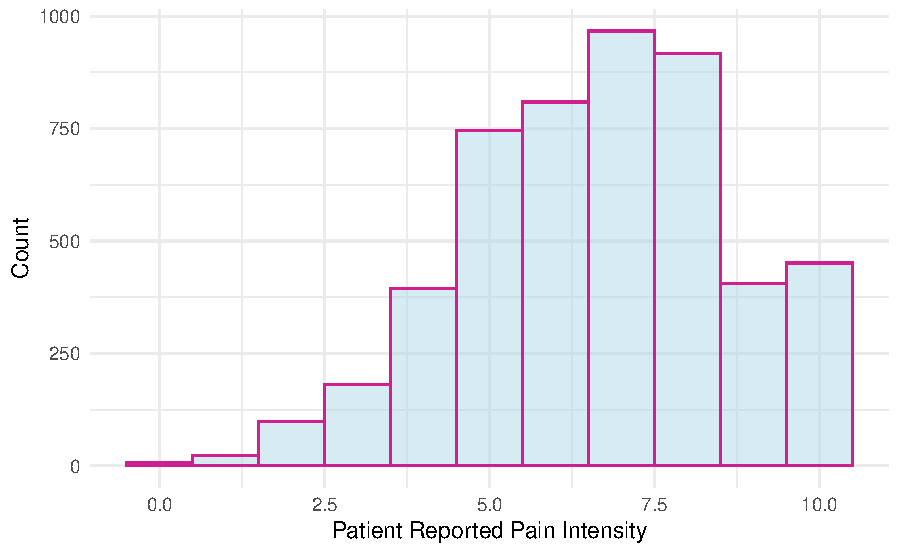
\includegraphics[width=1\textwidth,height=\textheight]{book/7_visualization_ggplot_files/figure-pdf/unnamed-chunk-5-1.pdf}

}

\end{figure}

Let's create another example. This time, I will create a histogram for
initial recorded pain level. To find the corresponding geom for the type
of plot we'd like to make, we can use the
\href{https://posit.co/wp-content/uploads/2022/10/data-visualization-1.pdf}{data
visualization cheat sheet from Posit}. The first page lists all the geom
options available along with what aesthetics we can set for each option.
For example, here we are interested in plotting the distribution of one
continuous variable, and under the \texttt{geom\_histogram()} function
we can see that we can specify \texttt{x} (the variable whose
distribution we want to plot) as well as \texttt{binwidth}, \texttt{y},
\texttt{alpha}, \texttt{color}, \texttt{fill}, \texttt{linetype},
\texttt{size}, and \texttt{weight}. By default, the \texttt{y} value in
a histogram is the count for each bin.

In the code below, you can see that we updated the color
(\texttt{color}), fill (\texttt{fill}), and opacity (\texttt{alpha}) of
our histogram bars and updated the number of bins to be 11 (to account
for the possible values 0-10). Additionally, we used the
\texttt{theme\_minimal()} function to change the background colors used.
You can find the available themes on the second page of the cheat sheet.
Try changing the theme of the above plot to \texttt{theme\_bw()}.

\begin{Shaded}
\begin{Highlighting}[]
\FunctionTok{ggplot}\NormalTok{(pain\_df)}\SpecialCharTok{+}
  \FunctionTok{geom\_histogram}\NormalTok{(}\FunctionTok{aes}\NormalTok{(}\AttributeTok{x=}\NormalTok{PAIN\_INTENSITY\_AVERAGE), }\AttributeTok{color=}\StringTok{"violetred"}\NormalTok{, }
                 \AttributeTok{fill=}\StringTok{"lightblue"}\NormalTok{, }\AttributeTok{alpha=}\FloatTok{0.5}\NormalTok{, }\AttributeTok{bins =} \DecValTok{11}\NormalTok{) }\SpecialCharTok{+}
  \FunctionTok{labs}\NormalTok{(}\AttributeTok{x=}\StringTok{"Patient Reported Pain Intensity"}\NormalTok{, }\AttributeTok{y=}\StringTok{"Count"}\NormalTok{)}\SpecialCharTok{+}
  \FunctionTok{theme\_minimal}\NormalTok{()}
\end{Highlighting}
\end{Shaded}

\begin{figure}[H]

{\centering 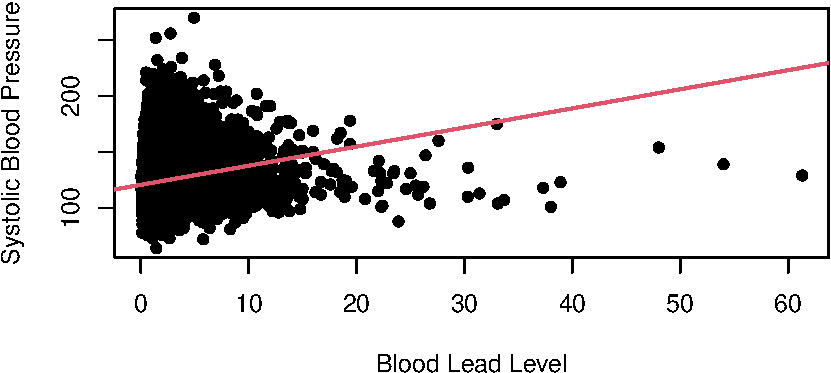
\includegraphics[width=1\textwidth,height=\textheight]{book/7_visualization_ggplot_files/figure-pdf/unnamed-chunk-6-1.pdf}

}

\end{figure}

\hypertarget{practice-question-13}{%
\subsection{Practice Question}\label{practice-question-13}}

Recreate the following plot.

\begin{Shaded}
\begin{Highlighting}[]
\CommentTok{\# Insert your solution here: }
\end{Highlighting}
\end{Shaded}

\hypertarget{adjusting-the-axes-and-aesthetics}{%
\section{Adjusting the Axes and
Aesthetics}\label{adjusting-the-axes-and-aesthetics}}

We can further control how each part specified in the aesthetic is
displayed using \textbf{scale} functions. For example, suppose that I
wanted to update the plot above. In particular, I first want to update
the x-axis to display all of the values 0 to 10 instead of 0, 2.5, 5,
etc.. To update the x-axis, I need to find the corresponding scale
function for x with continuous values. This function is
\texttt{scale\_x\_continuous()}, which allows me to specify limits
(\texttt{limits}), breaks (\texttt{breaks}), and labels
(\texttt{labels}). The scale functions can be found on the second sheet
of the cheat sheet. In this case, I just want to update the breaks to be
all integer values from 0 to 10.

\begin{Shaded}
\begin{Highlighting}[]
\FunctionTok{ggplot}\NormalTok{(pain\_df)}\SpecialCharTok{+}
  \FunctionTok{geom\_histogram}\NormalTok{(}\FunctionTok{aes}\NormalTok{(}\AttributeTok{x=}\NormalTok{PAIN\_INTENSITY\_AVERAGE), }\AttributeTok{color=}\StringTok{"violetred"}\NormalTok{, }
                 \AttributeTok{fill=}\StringTok{"lightblue"}\NormalTok{, }\AttributeTok{alpha=}\FloatTok{0.5}\NormalTok{, }\AttributeTok{bins =} \DecValTok{11}\NormalTok{) }\SpecialCharTok{+}
  \FunctionTok{labs}\NormalTok{(}\AttributeTok{x=}\StringTok{"Patient Reported Pain Intensity"}\NormalTok{, }\AttributeTok{y=}\StringTok{"Count"}\NormalTok{)}\SpecialCharTok{+}
  \FunctionTok{scale\_x\_continuous}\NormalTok{(}\AttributeTok{breaks=}\DecValTok{0}\SpecialCharTok{:}\DecValTok{10}\NormalTok{)}\SpecialCharTok{+}
  \FunctionTok{theme\_minimal}\NormalTok{()}
\end{Highlighting}
\end{Shaded}

\begin{figure}[H]

{\centering 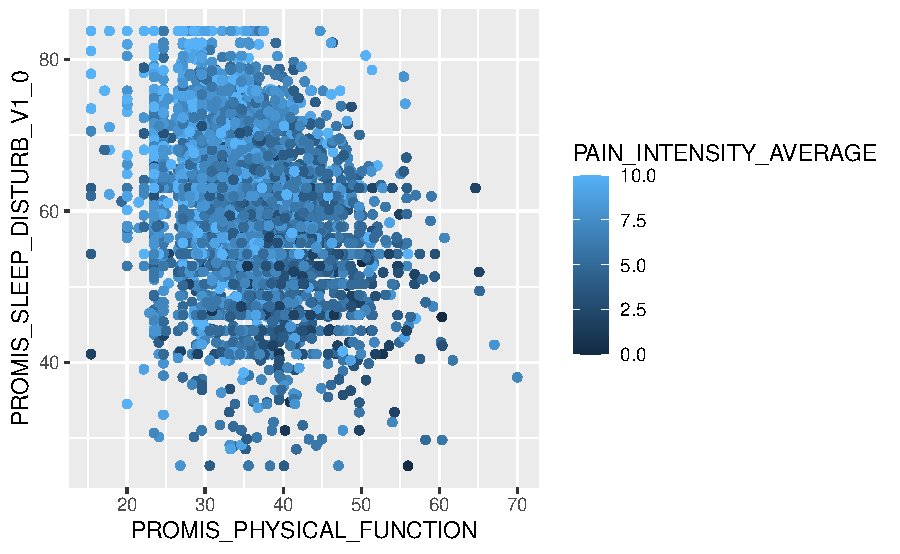
\includegraphics[width=1\textwidth,height=\textheight]{book/7_visualization_ggplot_files/figure-pdf/unnamed-chunk-8-1.pdf}

}

\end{figure}

Now, let's take a more complex example. The plot below shows each
patient's reported sleep disturbance vs.~physical function and colors
each point by their reported pain intensity. Since some points might
overlap in values, we added \texttt{position="jitter"} to the
\texttt{geom\_point()} function to jitter the points, which corresponds
to adding some random noise to each point's position. As it stands, this
plot is difficult to read. For example, the color of pain intensity
makes it hard to see how pain changes, and the legend title needs to be
simpler.

\begin{Shaded}
\begin{Highlighting}[]
\FunctionTok{ggplot}\NormalTok{(pain\_df)}\SpecialCharTok{+}
  \FunctionTok{geom\_point}\NormalTok{(}\FunctionTok{aes}\NormalTok{(}\AttributeTok{x=}\NormalTok{PROMIS\_PHYSICAL\_FUNCTION, }\AttributeTok{y=}\NormalTok{PROMIS\_SLEEP\_DISTURB\_V1\_0, }
                 \AttributeTok{color=}\NormalTok{PAIN\_INTENSITY\_AVERAGE), }\AttributeTok{position=}\StringTok{"jitter"}\NormalTok{)}
\end{Highlighting}
\end{Shaded}

\begin{figure}[H]

{\centering 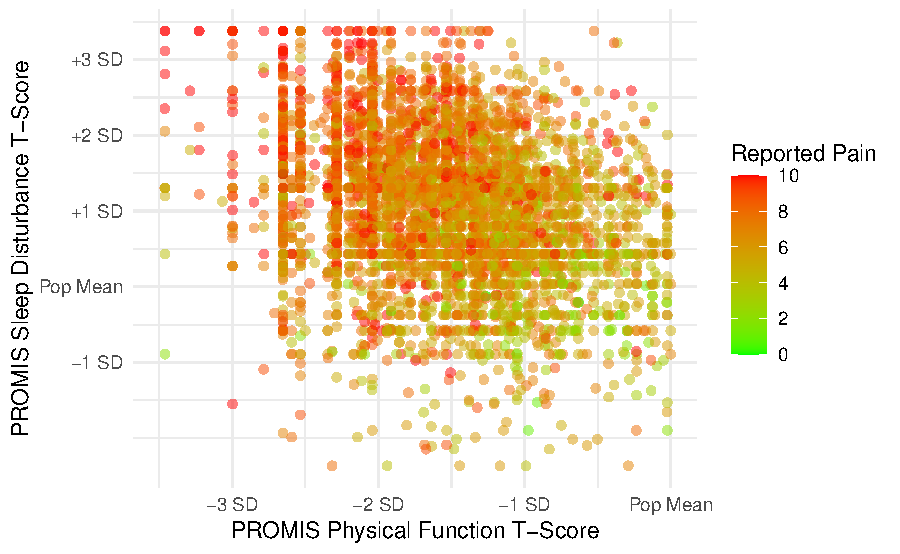
\includegraphics[width=1\textwidth,height=\textheight]{book/7_visualization_ggplot_files/figure-pdf/unnamed-chunk-9-1.pdf}

}

\end{figure}

Suppose that we wanted to visualize the pain intensity and sleep
disturbance for patients with below-average physical function. Note that
both sleep disturbance and physical function are reported as T-Scores,
meaning that the raw scores have been converted to a standardized score
with mean 50 and standard deviation 10 within the population. We can use
the scale functions to update our axes and labels to reflect this
information. As before, we need to use the
\texttt{scale\_x\_continuous()} function to update the x-axis for a
continuous variable. In this case, we update the limits (to restrict to
below average physical function), breaks, and labels. We similarly
update the y-axis.

Lastly, suppose we want to update the color aesthetic. As before, this
aesthetic corresponds to a continuous variable. The cheat sheet provides
several possible scale functions depending on how we want to specify the
color gradient. We choose the \texttt{scale\_color\_gradient()}
function, since this allows us to specify the low and high end colors.
We can also specify the breaks for the legend values similar to how we
specified the breaks for the x and y axes. The argument \texttt{name}
also allows us to rename this legend. The palette then converts this to
a continuous color gradient. Note that in contrast to the
\texttt{scale\_color\_gradient()} function that we chose to use for this
example, the functions \texttt{scale\_color\_gradient2()} and
\texttt{scale\_color\_gradientn()} allow you to specify more color
points in the gradient rather than just the two extreme colors.

We can observe that decreased physical function is associated with
higher sleep disturbance and that those with worse physical function and
worse sleep disturbance tend to have higher reported pain. Note that
this time we receive a warning message, which is because our axis limits
have cut off some points. To avoid this message, we could use the
function \texttt{coord\_cartesian()} to specify our limits which clips
the values rather than removing points outside the limits.

\begin{Shaded}
\begin{Highlighting}[]
\FunctionTok{ggplot}\NormalTok{(pain\_df)}\SpecialCharTok{+}
  \FunctionTok{geom\_point}\NormalTok{(}\FunctionTok{aes}\NormalTok{(}\AttributeTok{x=}\NormalTok{PROMIS\_PHYSICAL\_FUNCTION, }\AttributeTok{y=}\NormalTok{PROMIS\_SLEEP\_DISTURB\_V1\_0, }
                 \AttributeTok{color=}\NormalTok{PAIN\_INTENSITY\_AVERAGE), }\AttributeTok{position=}\StringTok{"jitter"}\NormalTok{, }\AttributeTok{alpha=}\FloatTok{0.5}\NormalTok{) }\SpecialCharTok{+}
  \FunctionTok{scale\_x\_continuous}\NormalTok{(}\AttributeTok{limits=}\FunctionTok{c}\NormalTok{(}\DecValTok{15}\NormalTok{,}\DecValTok{50}\NormalTok{), }\AttributeTok{breaks =} \FunctionTok{c}\NormalTok{(}\DecValTok{20}\NormalTok{, }\DecValTok{30}\NormalTok{, }\DecValTok{40}\NormalTok{, }\DecValTok{50}\NormalTok{), }
                     \AttributeTok{labels =} \FunctionTok{c}\NormalTok{(}\StringTok{"{-}3 SD"}\NormalTok{, }\StringTok{"{-}2 SD"}\NormalTok{, }\StringTok{"{-}1 SD"}\NormalTok{, }\StringTok{"Pop Mean"}\NormalTok{)) }\SpecialCharTok{+} 
  \FunctionTok{scale\_y\_continuous}\NormalTok{(}\AttributeTok{breaks =} \FunctionTok{c}\NormalTok{(}\DecValTok{40}\NormalTok{, }\DecValTok{50}\NormalTok{, }\DecValTok{60}\NormalTok{, }\DecValTok{70}\NormalTok{, }\DecValTok{80}\NormalTok{), }
                     \AttributeTok{labels =} \FunctionTok{c}\NormalTok{(}\StringTok{"{-}1 SD"}\NormalTok{, }\StringTok{"Pop Mean"}\NormalTok{, }\StringTok{"+1 SD"}\NormalTok{, }\StringTok{"+2 SD"}\NormalTok{, }
                                \StringTok{"+3 SD"}\NormalTok{)) }\SpecialCharTok{+}
  \FunctionTok{scale\_color\_gradient}\NormalTok{(}\AttributeTok{breaks=} \FunctionTok{seq}\NormalTok{(}\DecValTok{0}\NormalTok{,}\DecValTok{10}\NormalTok{,}\DecValTok{2}\NormalTok{), }\AttributeTok{low=}\StringTok{"green"}\NormalTok{, }\AttributeTok{high=}\StringTok{"red"}\NormalTok{, }
                       \StringTok{"Reported Pain"}\NormalTok{) }\SpecialCharTok{+}
  \FunctionTok{labs}\NormalTok{(}\AttributeTok{x=}\StringTok{"PROMIS Physical Function T{-}Score"}\NormalTok{, }
       \AttributeTok{y =} \StringTok{"PROMIS Sleep Disturbance T{-}Score"}\NormalTok{) }\SpecialCharTok{+} 
  \FunctionTok{theme\_minimal}\NormalTok{()}
\CommentTok{\#\textgreater{} Warning: Removed 121 rows containing missing values (\textasciigrave{}geom\_point()\textasciigrave{}).}
\end{Highlighting}
\end{Shaded}

\begin{figure}[H]

{\centering 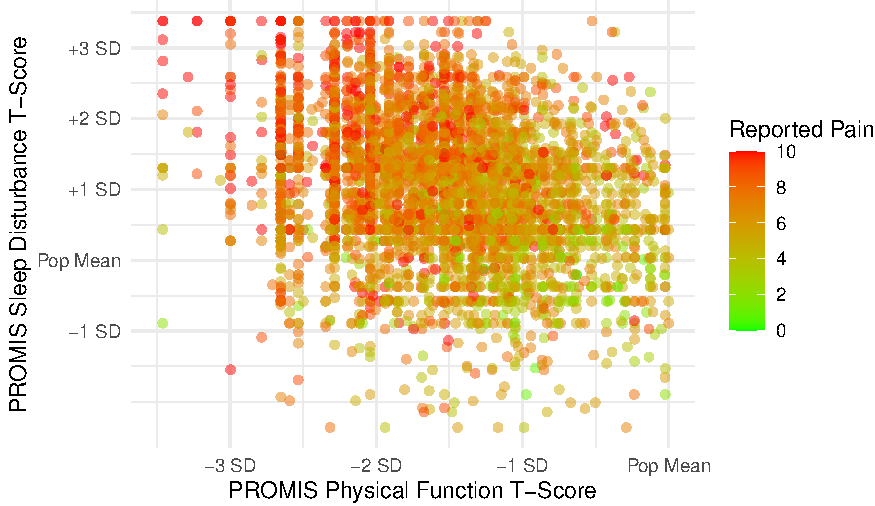
\includegraphics[width=1\textwidth,height=\textheight]{book/7_visualization_ggplot_files/figure-pdf/unnamed-chunk-10-1.pdf}

}

\end{figure}

We now demonstrate these scale functions for discrete variables. In the
example below, we first create a new race variable that has only three
categories since other groups have limited observations. We then create
a box plot for pain intensity by race. There are two discrete aesthetics
here: color and the y-axis. This plot shows a higher median pain for
black patients compared to other races.

\begin{Shaded}
\begin{Highlighting}[]
\NormalTok{pain\_df}\SpecialCharTok{$}\NormalTok{PAT\_RACE\_CAT }\OtherTok{\textless{}{-}} \FunctionTok{ifelse}\NormalTok{(pain\_df}\SpecialCharTok{$}\NormalTok{PAT\_RACE }\SpecialCharTok{\%in\%} \FunctionTok{c}\NormalTok{(}\StringTok{"BLACK"}\NormalTok{, }\StringTok{"WHITE"}\NormalTok{), }
\NormalTok{                               pain\_df}\SpecialCharTok{$}\NormalTok{PAT\_RACE, }\StringTok{"OTHER"}\NormalTok{)}
\NormalTok{pain\_df}\SpecialCharTok{$}\NormalTok{PAT\_RACE\_CAT }\OtherTok{\textless{}{-}} \FunctionTok{as.factor}\NormalTok{(pain\_df}\SpecialCharTok{$}\NormalTok{PAT\_RACE\_CAT)}
\end{Highlighting}
\end{Shaded}

\begin{Shaded}
\begin{Highlighting}[]
\FunctionTok{ggplot}\NormalTok{(pain\_df)}\SpecialCharTok{+}
  \FunctionTok{geom\_boxplot}\NormalTok{(}\FunctionTok{aes}\NormalTok{(}\AttributeTok{y=}\NormalTok{PAT\_RACE\_CAT, }\AttributeTok{x=}\NormalTok{PAIN\_INTENSITY\_AVERAGE, }
                   \AttributeTok{fill=}\NormalTok{PAT\_RACE\_CAT), }\AttributeTok{alpha=}\FloatTok{0.5}\NormalTok{) }\SpecialCharTok{+}
  \FunctionTok{theme\_minimal}\NormalTok{()}
\end{Highlighting}
\end{Shaded}

\begin{figure}[H]

{\centering 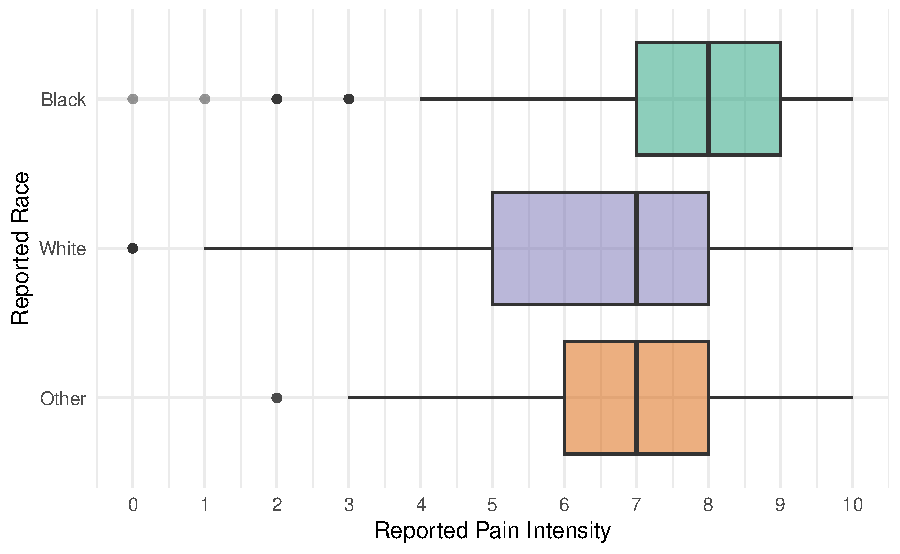
\includegraphics[width=1\textwidth,height=\textheight]{book/7_visualization_ggplot_files/figure-pdf/unnamed-chunk-12-1.pdf}

}

\end{figure}

The function \texttt{scale\_y\_discrete()} is the scale function that
corresponds to a discrete y-axis. In this case, we want to update the
order and labels of this y-axis. To update the order, we can either
refactor the variable using \texttt{factor()} prior to plotting or
update the \texttt{limits} argument of the scale function. The function
\texttt{scale\_fill\_brewer()} is a scale function to control the color
palette of a discrete variable used for the fill aesthetic. We use this
function to specify the color palette (\texttt{palette}) and to specify
that that we do not want a legend (\texttt{guide}). Since we do not have
a legend, we do not update the values and labels in this function.

\begin{Shaded}
\begin{Highlighting}[]
\FunctionTok{ggplot}\NormalTok{(pain\_df)}\SpecialCharTok{+}
  \FunctionTok{geom\_boxplot}\NormalTok{(}\FunctionTok{aes}\NormalTok{(}\AttributeTok{y=}\NormalTok{PAT\_RACE\_CAT, }\AttributeTok{x=}\NormalTok{PAIN\_INTENSITY\_AVERAGE, }
                   \AttributeTok{fill=}\NormalTok{PAT\_RACE\_CAT), }\AttributeTok{alpha=}\FloatTok{0.5}\NormalTok{) }\SpecialCharTok{+}
  \FunctionTok{scale\_x\_continuous}\NormalTok{(}\AttributeTok{breaks=}\FunctionTok{c}\NormalTok{(}\DecValTok{0}\SpecialCharTok{:}\DecValTok{10}\NormalTok{)) }\SpecialCharTok{+}
  \FunctionTok{scale\_y\_discrete}\NormalTok{(}\AttributeTok{limits=}\FunctionTok{c}\NormalTok{(}\StringTok{"OTHER"}\NormalTok{, }\StringTok{"WHITE"}\NormalTok{, }\StringTok{"BLACK"}\NormalTok{), }
                   \AttributeTok{labels=}\FunctionTok{c}\NormalTok{(}\StringTok{"Other"}\NormalTok{, }\StringTok{"White"}\NormalTok{, }\StringTok{"Black"}\NormalTok{)) }\SpecialCharTok{+}
  \FunctionTok{scale\_fill\_brewer}\NormalTok{(}\AttributeTok{palette=}\StringTok{"Dark2"}\NormalTok{, }\AttributeTok{guide=}\StringTok{"none"}\NormalTok{) }\SpecialCharTok{+}
  \FunctionTok{labs}\NormalTok{(}\AttributeTok{x=}\StringTok{"Reported Pain Intensity"}\NormalTok{, }\AttributeTok{y=}\StringTok{"Reported Race"}\NormalTok{) }\SpecialCharTok{+}
  \FunctionTok{theme\_minimal}\NormalTok{()}
\end{Highlighting}
\end{Shaded}

\begin{figure}[H]

{\centering 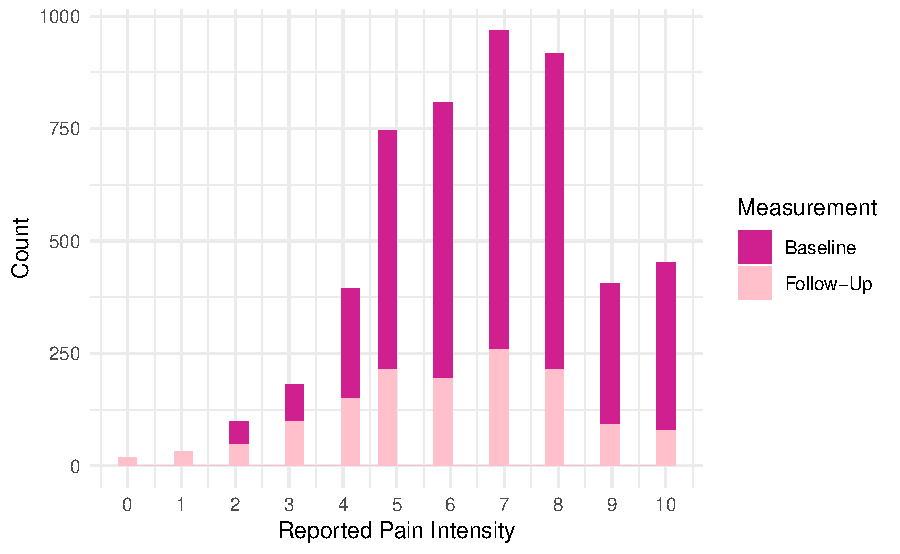
\includegraphics[width=1\textwidth,height=\textheight]{book/7_visualization_ggplot_files/figure-pdf/unnamed-chunk-13-1.pdf}

}

\end{figure}

The \textbf{RColorBrewer} package (Neuwirth 2022) contains several
default palettes to choose from, shown below. You can also create your
own palette using the \texttt{brewer.pal()} function from this package.
To visualize a palette you can use the available
\href{https://colorbrewer2.org/}{online tool}.

\begin{Shaded}
\begin{Highlighting}[]
\FunctionTok{library}\NormalTok{(RColorBrewer)}
\FunctionTok{display.brewer.all}\NormalTok{()}
\end{Highlighting}
\end{Shaded}

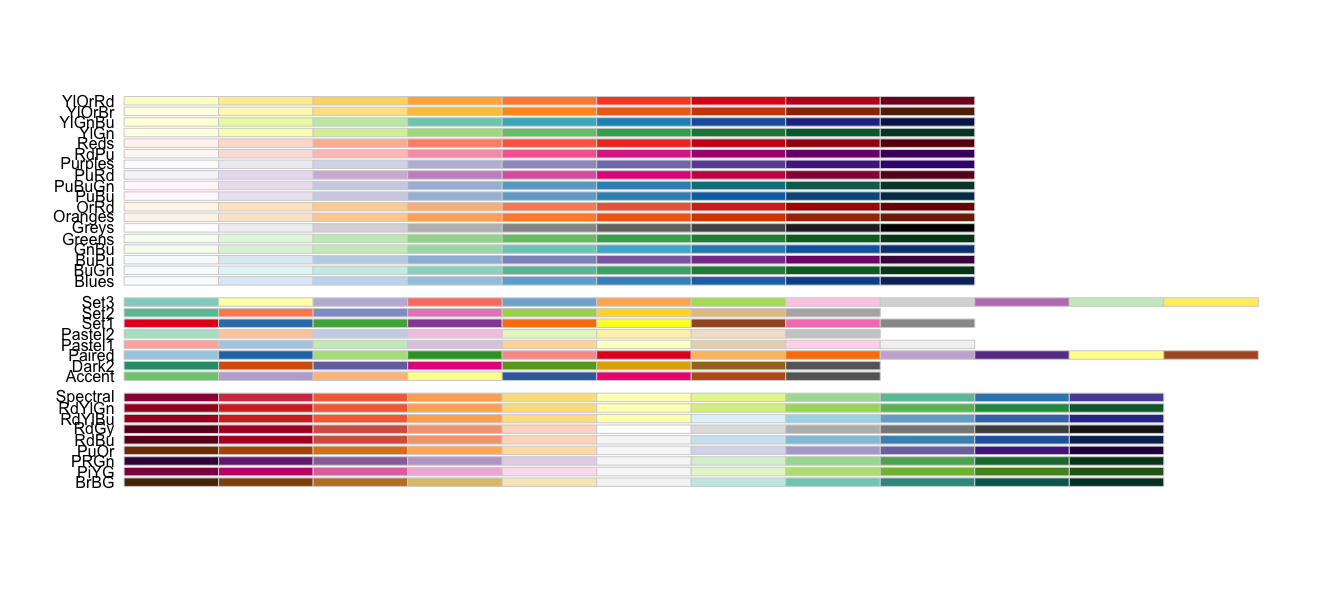
\includegraphics{book/images/7-palettes.png}\{\{width=``300pt''\}\}

Here is one more example of how you can use the scale functions - take a
look at the code below. We used two \texttt{geom\_histogram()} calls, or
layers, to plot a histogram of pain at baseline and at follow-up. This
allows us to visualize that pain at follow-up tends to be lower than at
baseline.

We also specify the fill to be by ``Baseline'' and ``Follow-up'' within
the aesthetic, even though this isn't a column in the data: this is a
sort of manual way to color the bars. We use the
\texttt{scale\_fill\_manual()} function to then specify the colors we
want to use for these two categories using the \texttt{values} argument.
We received three warnings when creating this plot! This is because we
have many NA values for follow-up and because we did not specify the bin
size for either histogram. C'est la vie.

\begin{Shaded}
\begin{Highlighting}[]
\FunctionTok{ggplot}\NormalTok{(pain\_df)}\SpecialCharTok{+}
  \FunctionTok{geom\_histogram}\NormalTok{(}\FunctionTok{aes}\NormalTok{(}\AttributeTok{x=}\NormalTok{PAIN\_INTENSITY\_AVERAGE, }\AttributeTok{fill=}\StringTok{"Baseline"}\NormalTok{)) }\SpecialCharTok{+}
  \FunctionTok{geom\_histogram}\NormalTok{(}\FunctionTok{aes}\NormalTok{(}\AttributeTok{x=}\NormalTok{PAIN\_INTENSITY\_AVERAGE.FOLLOW\_UP, }\AttributeTok{fill=}\StringTok{"Follow{-}Up"}\NormalTok{)) }\SpecialCharTok{+}
  \FunctionTok{scale\_x\_continuous}\NormalTok{(}\AttributeTok{breaks=}\FunctionTok{c}\NormalTok{(}\DecValTok{0}\SpecialCharTok{:}\DecValTok{10}\NormalTok{)) }\SpecialCharTok{+} 
  \FunctionTok{scale\_fill\_manual}\NormalTok{(}\AttributeTok{values=}\FunctionTok{c}\NormalTok{(}\StringTok{"violetred"}\NormalTok{, }\StringTok{"pink"}\NormalTok{), }\AttributeTok{name=}\StringTok{"Measurement"}\NormalTok{) }\SpecialCharTok{+}
  \FunctionTok{labs}\NormalTok{(}\AttributeTok{x=}\StringTok{"Reported Pain Intensity"}\NormalTok{, }\AttributeTok{y =} \StringTok{"Count"}\NormalTok{) }\SpecialCharTok{+}
  \FunctionTok{theme\_minimal}\NormalTok{()}
\CommentTok{\#\textgreater{} Warning: Removed 3604 rows containing non{-}finite values (\textasciigrave{}stat\_bin()\textasciigrave{}).}
\end{Highlighting}
\end{Shaded}

\begin{figure}[H]

{\centering 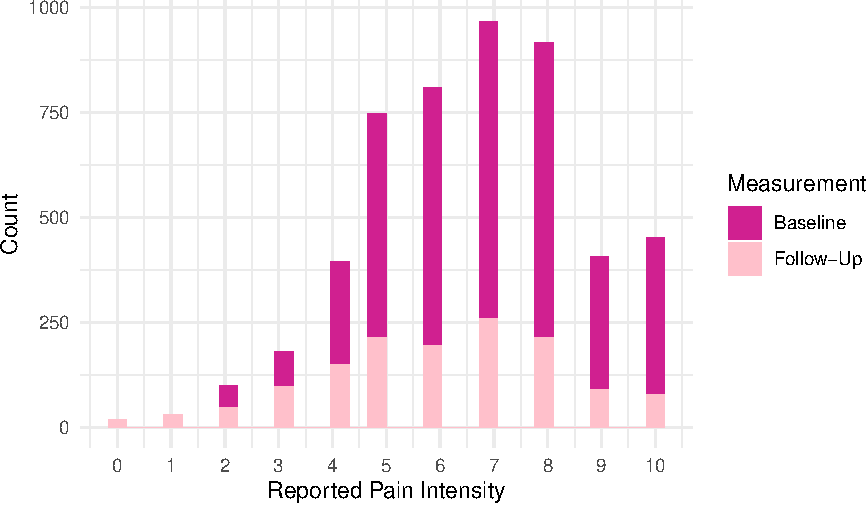
\includegraphics[width=1\textwidth,height=\textheight]{book/7_visualization_ggplot_files/figure-pdf/unnamed-chunk-15-1.pdf}

}

\end{figure}

\hypertarget{adding-groups}{%
\section{Adding Groups}\label{adding-groups}}

In the example above, we created two histograms using two calls to the
\texttt{geom\_histogram()} function, but there is another way to create
multiple layers like this when you have a variable that you want to
separate the geom layer on. For example, suppose we want to visualize
the distribution of physical function by whether someone has follow-up
information. Below we create the variable \texttt{HAS\_FOLLOW\_UP}
before using it in our aesthetic for \texttt{geom\_density()} as both
the color and group. In fact, we do not have to add the \texttt{group}
argument because as soon as we specify to R that we want to color the
density plots by this variable, R will create the grouping. Finally, we
update the legend for this grouping using the
\texttt{scale\_color\_discrete()} function, since the discrete variable
\texttt{HAS\_FOLLOW\_UP} specifies the color.

\begin{Shaded}
\begin{Highlighting}[]
\NormalTok{pain\_df}\SpecialCharTok{$}\NormalTok{HAS\_FOLLOW\_UP }\OtherTok{\textless{}{-}} \SpecialCharTok{!}\FunctionTok{is.na}\NormalTok{(pain\_df}\SpecialCharTok{$}\NormalTok{PAIN\_INTENSITY\_AVERAGE.FOLLOW\_UP)}
\FunctionTok{ggplot}\NormalTok{(pain\_df)}\SpecialCharTok{+}
  \FunctionTok{geom\_density}\NormalTok{(}\FunctionTok{aes}\NormalTok{(}\AttributeTok{x=}\NormalTok{PROMIS\_PHYSICAL\_FUNCTION, }\AttributeTok{group=}\NormalTok{HAS\_FOLLOW\_UP, }
                   \AttributeTok{color=}\NormalTok{HAS\_FOLLOW\_UP)) }\SpecialCharTok{+}
  \FunctionTok{scale\_x\_continuous}\NormalTok{(}\AttributeTok{breaks=}\FunctionTok{c}\NormalTok{(}\DecValTok{0}\SpecialCharTok{:}\DecValTok{10}\NormalTok{)) }\SpecialCharTok{+} 
  \FunctionTok{scale\_color\_discrete}\NormalTok{(}\AttributeTok{name=}\StringTok{"Follow{-}Up"}\NormalTok{, }\AttributeTok{labels =} \FunctionTok{c}\NormalTok{(}\StringTok{"No"}\NormalTok{, }\StringTok{"Yes"}\NormalTok{)) }\SpecialCharTok{+}
  \FunctionTok{labs}\NormalTok{(}\AttributeTok{x=}\StringTok{"PROMIS Physical Function T{-}Score"}\NormalTok{, }\AttributeTok{y=}\StringTok{"Estimated Density"}\NormalTok{) }\SpecialCharTok{+}
  \FunctionTok{theme\_minimal}\NormalTok{()}
\end{Highlighting}
\end{Shaded}

\begin{figure}[H]

{\centering 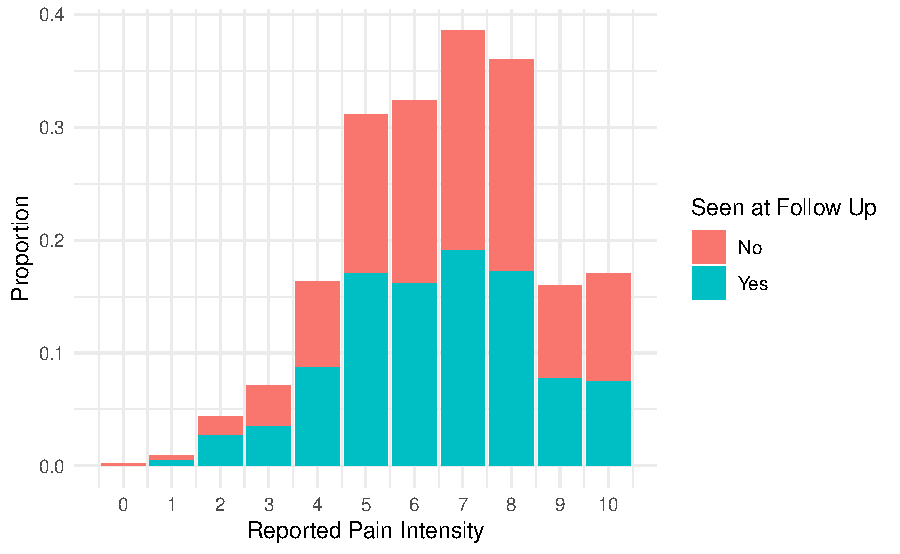
\includegraphics[width=1\textwidth,height=\textheight]{book/7_visualization_ggplot_files/figure-pdf/unnamed-chunk-16-1.pdf}

}

\end{figure}

Let's try another example. Suppose that we want to find the distribution
of initial overall pain by those that do and do not have follow up. In
this case, we want to plot the proportion of each pain score for each
group rather than comparing counts. We first need to find these
proportions, which we do by grouping and summarizing over our data.

\begin{Shaded}
\begin{Highlighting}[]
\NormalTok{pain\_df\_grp }\OtherTok{\textless{}{-}}\NormalTok{ pain\_df }\SpecialCharTok{\%\textgreater{}\%}
  \FunctionTok{group\_by}\NormalTok{(HAS\_FOLLOW\_UP, PAIN\_INTENSITY\_AVERAGE) }\SpecialCharTok{\%\textgreater{}\%}
  \FunctionTok{summarize}\NormalTok{(}\AttributeTok{tot =} \FunctionTok{n}\NormalTok{()) }\SpecialCharTok{\%\textgreater{}\%}
  \FunctionTok{mutate}\NormalTok{(}\AttributeTok{prop =}\NormalTok{ tot}\SpecialCharTok{/}\FunctionTok{sum}\NormalTok{(tot)) }\SpecialCharTok{\%\textgreater{}\%}
  \FunctionTok{ungroup}\NormalTok{()}
\FunctionTok{head}\NormalTok{(pain\_df\_grp)}
\CommentTok{\#\textgreater{} \# A tibble: 6 x 4}
\CommentTok{\#\textgreater{}   HAS\_FOLLOW\_UP PAIN\_INTENSITY\_AVERAGE   tot    prop}
\CommentTok{\#\textgreater{}   \textless{}lgl\textgreater{}                          \textless{}dbl\textgreater{} \textless{}int\textgreater{}   \textless{}dbl\textgreater{}}
\CommentTok{\#\textgreater{} 1 FALSE                              0     8 0.00222}
\CommentTok{\#\textgreater{} 2 FALSE                              1    16 0.00444}
\CommentTok{\#\textgreater{} 3 FALSE                              2    62 0.0172 }
\CommentTok{\#\textgreater{} 4 FALSE                              3   132 0.0366 }
\CommentTok{\#\textgreater{} 5 FALSE                              4   273 0.0757 }
\CommentTok{\#\textgreater{} \# i 1 more row}
\end{Highlighting}
\end{Shaded}

We can now use the \texttt{geom\_col()} function to create a bar plot of
these proportions. By default, this function will stack the bars on top
of each other when there is grouping. Try adding
\texttt{position="dodge"} to the \texttt{geom\_col()} function to place
the bars side by side instead of on top of each other.

\begin{Shaded}
\begin{Highlighting}[]
\FunctionTok{ggplot}\NormalTok{(pain\_df\_grp)}\SpecialCharTok{+}
  \FunctionTok{geom\_col}\NormalTok{(}\FunctionTok{aes}\NormalTok{(}\AttributeTok{x=}\NormalTok{PAIN\_INTENSITY\_AVERAGE, }\AttributeTok{y=}\NormalTok{prop, }\AttributeTok{fill=}\NormalTok{HAS\_FOLLOW\_UP)) }\SpecialCharTok{+}
  \FunctionTok{scale\_x\_continuous}\NormalTok{(}\AttributeTok{breaks=}\FunctionTok{c}\NormalTok{(}\DecValTok{0}\SpecialCharTok{:}\DecValTok{10}\NormalTok{)) }\SpecialCharTok{+} 
  \FunctionTok{scale\_fill\_discrete}\NormalTok{(}\AttributeTok{name=}\StringTok{"Seen at Follow Up"}\NormalTok{, }\AttributeTok{labels=}\FunctionTok{c}\NormalTok{(}\StringTok{"No"}\NormalTok{, }\StringTok{"Yes"}\NormalTok{)) }\SpecialCharTok{+}
  \FunctionTok{labs}\NormalTok{(}\AttributeTok{x=}\StringTok{"Reported Pain Intensity"}\NormalTok{, }\AttributeTok{y =} \StringTok{"Proportion"}\NormalTok{) }\SpecialCharTok{+}
  \FunctionTok{theme\_minimal}\NormalTok{()}
\end{Highlighting}
\end{Shaded}

\begin{figure}[H]

{\centering 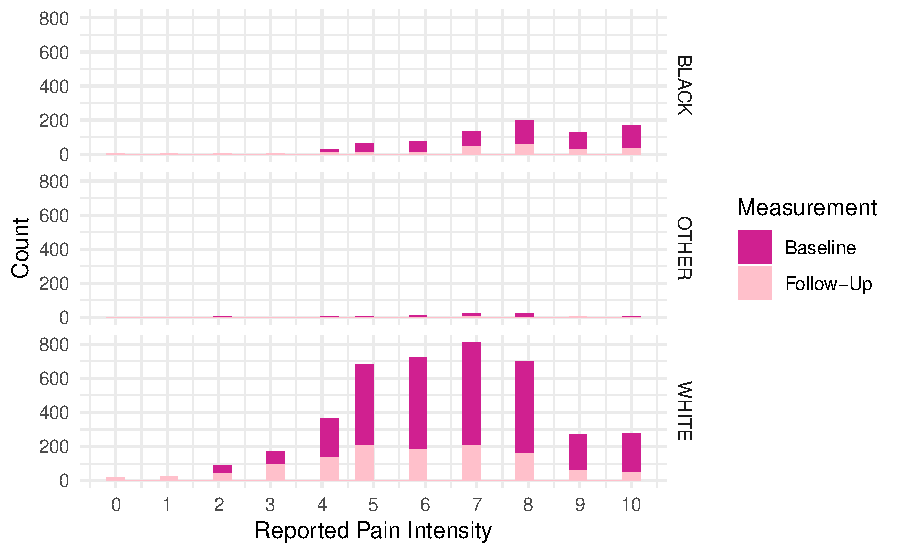
\includegraphics[width=1\textwidth,height=\textheight]{book/7_visualization_ggplot_files/figure-pdf/unnamed-chunk-18-1.pdf}

}

\end{figure}

\hypertarget{practice-question-14}{%
\subsection{Practice Question}\label{practice-question-14}}

Recreate the following plot.

\begin{Shaded}
\begin{Highlighting}[]
\CommentTok{\# Insert your solution here:}
\end{Highlighting}
\end{Shaded}

Another way to visualize data by group is to add a facet wrap to your
ggplot object. Facets divide a plot into subplots based on one or more
discrete variable values. We can either arrange these plots as a grid
where the rows and/or columns correspond to the variables we are
grouping by using \texttt{facet\_grid()} and specifying the column and
row variables using the \texttt{col} and \texttt{row} arguments
respectively. Or we can wrap the plots into a rectangular format using
\texttt{facet\_wrap()} and specifying the columns using the
\texttt{facet} argument. Below, we take one of our previous plots and
add a facet grid where the columns of the grid are given by racial
group. If we had set \texttt{row=vars(PAT\_RACE\_CAT)}, then this would
stack the plots vertically. Note that we have to specify the variables
inside the \texttt{vars()} function.

\begin{Shaded}
\begin{Highlighting}[]
\FunctionTok{ggplot}\NormalTok{(pain\_df)}\SpecialCharTok{+}
  \FunctionTok{geom\_histogram}\NormalTok{(}\FunctionTok{aes}\NormalTok{(}\AttributeTok{x=}\NormalTok{PAIN\_INTENSITY\_AVERAGE, }\AttributeTok{fill=}\StringTok{"Baseline"}\NormalTok{)) }\SpecialCharTok{+}
  \FunctionTok{geom\_histogram}\NormalTok{(}\FunctionTok{aes}\NormalTok{(}\AttributeTok{x=}\NormalTok{PAIN\_INTENSITY\_AVERAGE.FOLLOW\_UP, }\AttributeTok{fill=}\StringTok{"Follow{-}Up"}\NormalTok{)) }\SpecialCharTok{+}
  \FunctionTok{scale\_x\_continuous}\NormalTok{(}\AttributeTok{breaks=}\FunctionTok{c}\NormalTok{(}\DecValTok{0}\SpecialCharTok{:}\DecValTok{10}\NormalTok{)) }\SpecialCharTok{+} 
  \FunctionTok{scale\_fill\_manual}\NormalTok{(}\AttributeTok{values=}\FunctionTok{c}\NormalTok{(}\StringTok{"violetred"}\NormalTok{, }\StringTok{"pink"}\NormalTok{), }\AttributeTok{name=}\StringTok{"Measurement"}\NormalTok{) }\SpecialCharTok{+}
  \FunctionTok{labs}\NormalTok{(}\AttributeTok{x=}\StringTok{"Reported Pain Intensity"}\NormalTok{, }\AttributeTok{y =} \StringTok{"Count"}\NormalTok{) }\SpecialCharTok{+}
  \FunctionTok{facet\_grid}\NormalTok{(}\AttributeTok{row=}\FunctionTok{vars}\NormalTok{(PAT\_RACE\_CAT))}\SpecialCharTok{+}
  \FunctionTok{theme\_minimal}\NormalTok{()}
\CommentTok{\#\textgreater{} Warning: Removed 3604 rows containing non{-}finite values (\textasciigrave{}stat\_bin()\textasciigrave{}).}
\end{Highlighting}
\end{Shaded}

\begin{figure}[H]

{\centering 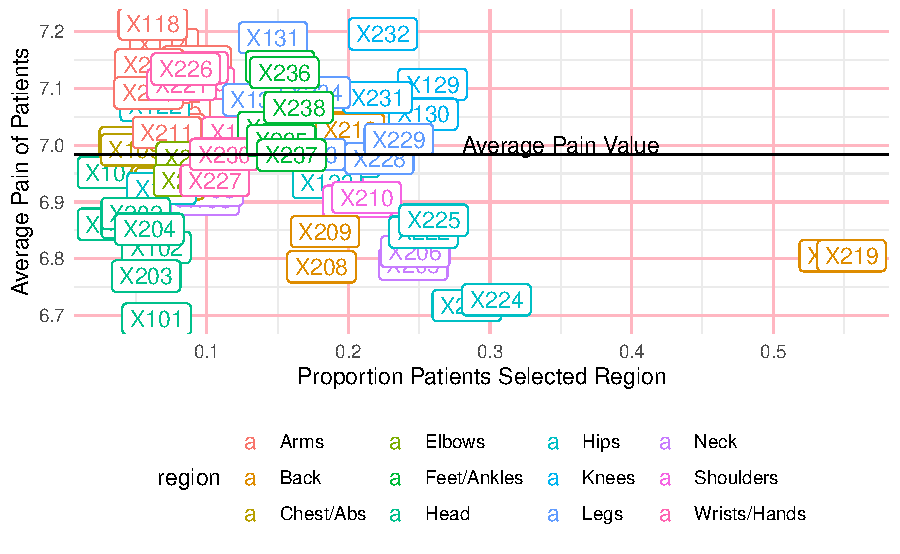
\includegraphics[width=1\textwidth,height=\textheight]{book/7_visualization_ggplot_files/figure-pdf/unnamed-chunk-20-1.pdf}

}

\end{figure}

\hypertarget{extra-options}{%
\section{Extra Options}\label{extra-options}}

To create our final plot, we will demonstrate some extra features we
haven't covered so far. To create this plot, we first find the number of
participants who selected each body region as well as the average pain
intensity for those patients. We also classify each body part region
into larger groups.

\begin{Shaded}
\begin{Highlighting}[]
\NormalTok{pain\_body\_map }\OtherTok{\textless{}{-}} \FunctionTok{data.frame}\NormalTok{(}\AttributeTok{part =} \FunctionTok{names}\NormalTok{(pain\_df)[}\DecValTok{2}\SpecialCharTok{:}\DecValTok{75}\NormalTok{])}
\NormalTok{pain\_body\_map}\SpecialCharTok{$}\NormalTok{num\_patients }\OtherTok{\textless{}{-}} \FunctionTok{colSums}\NormalTok{(pain\_df[,}\DecValTok{2}\SpecialCharTok{:}\DecValTok{75}\NormalTok{])}
\NormalTok{pain\_body\_map}\SpecialCharTok{$}\NormalTok{perc\_patients }\OtherTok{\textless{}{-}}\NormalTok{ pain\_body\_map}\SpecialCharTok{$}\NormalTok{num\_patients}\SpecialCharTok{/}\FunctionTok{nrow}\NormalTok{(pain\_df)}
\NormalTok{pain\_body\_map}\SpecialCharTok{$}\NormalTok{avg\_pain }\OtherTok{\textless{}{-}} \FunctionTok{colSums}\NormalTok{(pain\_df[,}\DecValTok{2}\SpecialCharTok{:}\DecValTok{75}\NormalTok{] }\SpecialCharTok{*} 
\NormalTok{                                pain\_df}\SpecialCharTok{$}\NormalTok{PAIN\_INTENSITY\_AVERAGE) }\SpecialCharTok{/}
\NormalTok{  pain\_body\_map}\SpecialCharTok{$}\NormalTok{num\_patients}
\NormalTok{pain\_body\_map }\OtherTok{\textless{}{-}}\NormalTok{ pain\_body\_map }\SpecialCharTok{\%\textgreater{}\%} 
    \FunctionTok{mutate}\NormalTok{( }\AttributeTok{region =} \FunctionTok{case\_when}\NormalTok{(}
\NormalTok{    part }\SpecialCharTok{\%in\%} \FunctionTok{c}\NormalTok{(}\StringTok{"X208"}\NormalTok{, }\StringTok{"X209"}\NormalTok{, }\StringTok{"X218"}\NormalTok{,}\StringTok{"X219"}\NormalTok{,}\StringTok{"X212"}\NormalTok{,}\StringTok{"X213"}\NormalTok{) }\SpecialCharTok{\textasciitilde{}} \StringTok{"Back"}\NormalTok{,}
\NormalTok{    part }\SpecialCharTok{\%in\%} \FunctionTok{c}\NormalTok{(}\StringTok{"X105"}\NormalTok{, }\StringTok{"X106"}\NormalTok{, }\StringTok{"X205"}\NormalTok{,}\StringTok{"X206"}\NormalTok{) }\SpecialCharTok{\textasciitilde{}} \StringTok{"Neck"}\NormalTok{,}
\NormalTok{    part }\SpecialCharTok{\%in\%} \FunctionTok{c}\NormalTok{(}\StringTok{"X107"}\NormalTok{, }\StringTok{"X110"}\NormalTok{, }\StringTok{"X207"}\NormalTok{,}\StringTok{"X210"}\NormalTok{) }\SpecialCharTok{\textasciitilde{}} \StringTok{"Shoulders"}\NormalTok{,}
\NormalTok{    part }\SpecialCharTok{\%in\%} \FunctionTok{c}\NormalTok{(}\StringTok{"X108"}\NormalTok{,}\StringTok{"X109"}\NormalTok{,}\StringTok{"X112"}\NormalTok{,}\StringTok{"X113"}\NormalTok{) }\SpecialCharTok{\textasciitilde{}} \StringTok{"Chest/Abs"}\NormalTok{,}
\NormalTok{    part }\SpecialCharTok{\%in\%} \FunctionTok{c}\NormalTok{(}\StringTok{"X126"}\NormalTok{,}\StringTok{"X127"}\NormalTok{,}\StringTok{"X228"}\NormalTok{,}\StringTok{"X229"}\NormalTok{,}
                \StringTok{"X131"}\NormalTok{,}\StringTok{"X132"}\NormalTok{,}\StringTok{"X233"}\NormalTok{,}\StringTok{"X234"}\NormalTok{)}\SpecialCharTok{\textasciitilde{}}\StringTok{"Legs"}\NormalTok{,}
\NormalTok{    part }\SpecialCharTok{\%in\%} \FunctionTok{c}\NormalTok{(}\StringTok{"X111"}\NormalTok{,}\StringTok{"X114"}\NormalTok{,}\StringTok{"X211"}\NormalTok{,}\StringTok{"X214"}\NormalTok{,}\StringTok{"X115"}\NormalTok{,}\StringTok{"X116"}\NormalTok{,}
                \StringTok{"X117"}\NormalTok{,}\StringTok{"X118"}\NormalTok{,}\StringTok{"X217"}\NormalTok{,}\StringTok{"X220"}\NormalTok{)}\SpecialCharTok{\textasciitilde{}}\StringTok{"Arms"}\NormalTok{,}
\NormalTok{    part }\SpecialCharTok{\%in\%} \FunctionTok{c}\NormalTok{(}\StringTok{"X119"}\NormalTok{,}\StringTok{"X124"}\NormalTok{,}\StringTok{"X221"}\NormalTok{,}\StringTok{"X226"}\NormalTok{,}\StringTok{"X125"}\NormalTok{,}\StringTok{"X128"}\NormalTok{,}
                \StringTok{"X227"}\NormalTok{,}\StringTok{"X230"}\NormalTok{)}\SpecialCharTok{\textasciitilde{}}\StringTok{"Wrists/Hands"}\NormalTok{,}
\NormalTok{    part }\SpecialCharTok{\%in\%} \FunctionTok{c}\NormalTok{(}\StringTok{"X215"}\NormalTok{,}\StringTok{"X216"}\NormalTok{)}\SpecialCharTok{\textasciitilde{}}\StringTok{"Elbows"}\NormalTok{,}
\NormalTok{    part }\SpecialCharTok{\%in\%} \FunctionTok{c}\NormalTok{(}\StringTok{"X135"}\NormalTok{,}\StringTok{"X136"}\NormalTok{,}\StringTok{"X237"}\NormalTok{,}\StringTok{"X238"}\NormalTok{,}\StringTok{"X133"}\NormalTok{,}\StringTok{"X134"}\NormalTok{,}
                \StringTok{"X235"}\NormalTok{,}\StringTok{"X236"}\NormalTok{)}\SpecialCharTok{\textasciitilde{}}\StringTok{"Feet/Ankles"}\NormalTok{,}
\NormalTok{    part }\SpecialCharTok{\%in\%} \FunctionTok{c}\NormalTok{(}\StringTok{"X129"}\NormalTok{,}\StringTok{"X130"}\NormalTok{,}\StringTok{"X231"}\NormalTok{,}\StringTok{"X232"}\NormalTok{)}\SpecialCharTok{\textasciitilde{}}\StringTok{"Knees"}\NormalTok{,}
\NormalTok{    part }\SpecialCharTok{\%in\%} \FunctionTok{c}\NormalTok{(}\StringTok{"X101"}\NormalTok{,}\StringTok{"X102"}\NormalTok{,}\StringTok{"X103"}\NormalTok{,}\StringTok{"X104"}\NormalTok{,}\StringTok{"X201"}\NormalTok{,}\StringTok{"X203"}\NormalTok{,}
                \StringTok{"X202"}\NormalTok{,}\StringTok{"X204"}\NormalTok{)}\SpecialCharTok{\textasciitilde{}}\StringTok{"Head"}\NormalTok{,}
\NormalTok{    part }\SpecialCharTok{\%in\%} \FunctionTok{c}\NormalTok{(}\StringTok{"X120"}\NormalTok{,}\StringTok{"X121"}\NormalTok{,}\StringTok{"X122"}\NormalTok{,}\StringTok{"X123"}\NormalTok{,}\StringTok{"X222"}\NormalTok{,}\StringTok{"X223"}\NormalTok{,}
                \StringTok{"X224"}\NormalTok{,}\StringTok{"X225"}\NormalTok{)}\SpecialCharTok{\textasciitilde{}}\StringTok{"Hips"}\NormalTok{))}
    
\FunctionTok{head}\NormalTok{(pain\_body\_map)}
\CommentTok{\#\textgreater{}   part num\_patients perc\_patients avg\_pain region}
\CommentTok{\#\textgreater{} 1 X101          323        0.0646     6.69   Head}
\CommentTok{\#\textgreater{} 2 X102          322        0.0644     6.82   Head}
\CommentTok{\#\textgreater{} 3 X103          165        0.0330     6.86   Head}
\CommentTok{\#\textgreater{} 4 X104          165        0.0330     6.95   Head}
\CommentTok{\#\textgreater{} 5 X105          493        0.0986     6.90   Neck}
\CommentTok{\#\textgreater{} 6 X106          507        0.1014     6.92   Neck}
\end{Highlighting}
\end{Shaded}

Within the theme we've chosen, we are able to update any of the theme
options (see \texttt{?theme}). Below we use the \texttt{theme()}
function to update the legend position to the bottom and the grid lines
to light pink. Additionally, we add a horizontal line using the
\texttt{geom\_hline()} function (\texttt{geom\_vline()} and
\texttt{geom\_abline()} can add vertical or diagonal lines respectively)
and add a text annotation using the \texttt{annotate()} function. The
resulting plot below shows the average pain value for each body part as
well as the proportion of patients who categorized it as being painful.

\begin{Shaded}
\begin{Highlighting}[]
\FunctionTok{ggplot}\NormalTok{(pain\_body\_map) }\SpecialCharTok{+}
  \FunctionTok{geom\_label}\NormalTok{(}\FunctionTok{aes}\NormalTok{(}\AttributeTok{x=}\NormalTok{perc\_patients, }\AttributeTok{y=}\NormalTok{avg\_pain, }\AttributeTok{label=}\NormalTok{part, }\AttributeTok{color=}\NormalTok{region)) }\SpecialCharTok{+} 
  \FunctionTok{geom\_hline}\NormalTok{(}\AttributeTok{yintercept=}\FunctionTok{mean}\NormalTok{(pain\_body\_map}\SpecialCharTok{$}\NormalTok{avg\_pain)) }\SpecialCharTok{+}
  \FunctionTok{annotate}\NormalTok{(}\AttributeTok{geom=}\StringTok{"text"}\NormalTok{, }\AttributeTok{label=}\StringTok{"Average Pain Value"}\NormalTok{, }\AttributeTok{x=}\FloatTok{0.35}\NormalTok{, }\AttributeTok{y=}\FloatTok{7.0}\NormalTok{) }\SpecialCharTok{+} 
  \FunctionTok{labs}\NormalTok{(}\AttributeTok{x=}\StringTok{"Proportion Patients Selected Region"}\NormalTok{, }\AttributeTok{y=}\StringTok{"Average Pain of Patients"}\NormalTok{) }\SpecialCharTok{+}
  \FunctionTok{theme\_minimal}\NormalTok{()}\SpecialCharTok{+}
  \FunctionTok{theme}\NormalTok{(}\AttributeTok{legend.position=}\StringTok{"bottom"}\NormalTok{, }
        \AttributeTok{panel.grid.major =} \FunctionTok{element\_line}\NormalTok{(}\AttributeTok{colour =} \StringTok{"lightpink"}\NormalTok{))}
\end{Highlighting}
\end{Shaded}

\begin{figure}[H]

{\centering \includegraphics[width=1\textwidth,height=\textheight]{book/7_visualization_ggplot_files/figure-pdf/unnamed-chunk-22-1.pdf}

}

\end{figure}

So far we have not saved any of our figures as objects. Below, I create
two plots and save them as objects named \texttt{p1} and \texttt{p2}. If
we want to save these plots, we can use the \texttt{ggsave()} function,
which saves the last plot generated under the file name provided.
Additionally, I can use the \textbf{patchwork} package to incorporate
multiple plots together. A \texttt{+} between plots puts them side by
side whereas \texttt{/} stacks them.

\begin{Shaded}
\begin{Highlighting}[]
\NormalTok{p1 }\OtherTok{\textless{}{-}} \FunctionTok{ggplot}\NormalTok{(pain\_body\_map) }\SpecialCharTok{+}
  \FunctionTok{geom\_label}\NormalTok{(}\FunctionTok{aes}\NormalTok{(}\AttributeTok{x=}\NormalTok{perc\_patients, }\AttributeTok{y=}\NormalTok{avg\_pain, }\AttributeTok{label=}\NormalTok{part, }\AttributeTok{color=}\NormalTok{region)) }\SpecialCharTok{+} 
  \FunctionTok{geom\_hline}\NormalTok{(}\AttributeTok{yintercept=}\FunctionTok{mean}\NormalTok{(pain\_body\_map}\SpecialCharTok{$}\NormalTok{avg\_pain)) }\SpecialCharTok{+}
  \FunctionTok{annotate}\NormalTok{(}\AttributeTok{geom=}\StringTok{"text"}\NormalTok{, }\AttributeTok{label=}\StringTok{"Average Pain Value"}\NormalTok{, }\AttributeTok{x=}\FloatTok{0.35}\NormalTok{, }\AttributeTok{y=}\FloatTok{7.0}\NormalTok{) }\SpecialCharTok{+} 
  \FunctionTok{labs}\NormalTok{(}\AttributeTok{x=}\StringTok{"Proportion Patients Selected Region"}\NormalTok{, }\AttributeTok{y=}\StringTok{"Average Pain of Patients"}\NormalTok{) }\SpecialCharTok{+}
  \FunctionTok{theme\_minimal}\NormalTok{()}\SpecialCharTok{+}
  \FunctionTok{theme}\NormalTok{(}\AttributeTok{legend.position=}\StringTok{"bottom"}\NormalTok{, }
        \AttributeTok{panel.grid.major =} \FunctionTok{element\_line}\NormalTok{(}\AttributeTok{colour =} \StringTok{"lightpink"}\NormalTok{))}

\NormalTok{p2 }\OtherTok{\textless{}{-}} \FunctionTok{ggplot}\NormalTok{(pain\_body\_map) }\SpecialCharTok{+}
  \FunctionTok{geom\_histogram}\NormalTok{(}\FunctionTok{aes}\NormalTok{(}\AttributeTok{x=}\NormalTok{perc\_patients), }\AttributeTok{color=}\StringTok{"violetred"}\NormalTok{, }\AttributeTok{fill=}\StringTok{"lightpink"}\NormalTok{) }\SpecialCharTok{+} 
  \FunctionTok{labs}\NormalTok{(}\AttributeTok{x=}\StringTok{"Proportion of Patients Selected Region"}\NormalTok{, }\AttributeTok{y=}\StringTok{"Count"}\NormalTok{) }\SpecialCharTok{+}
  \FunctionTok{theme\_minimal}\NormalTok{()}\SpecialCharTok{+}
  \FunctionTok{theme}\NormalTok{(}\AttributeTok{panel.grid.major =} \FunctionTok{element\_line}\NormalTok{(}\AttributeTok{colour =} \StringTok{"lightpink"}\NormalTok{))}
\end{Highlighting}
\end{Shaded}

\begin{Shaded}
\begin{Highlighting}[]
\NormalTok{p1}\SpecialCharTok{/}\NormalTok{p2}
\end{Highlighting}
\end{Shaded}

\begin{figure}[H]

{\centering \includegraphics[width=1\textwidth,height=\textheight]{book/7_visualization_ggplot_files/figure-pdf/unnamed-chunk-24-1.pdf}

}

\end{figure}

\begin{Shaded}
\begin{Highlighting}[]
\FunctionTok{ggsave}\NormalTok{(}\StringTok{"images/myplot.png"}\NormalTok{) }
\end{Highlighting}
\end{Shaded}

\hypertarget{exercises-5}{%
\section{Exercises}\label{exercises-5}}

For this chapter's exercises, use the \texttt{covidcases} data set that
we first introduced in Chapter~\ref{sec-transformations-summaries} to
recreate the plots below. These are complex plots, so try to build them
up one step at a time and just try to get as close as possible to the
given examples.

\begin{enumerate}
\def\labelenumi{\arabic{enumi}.}
\tightlist
\item
  Replicate the plot in Figure~\ref{fig-q1}, which shows the weekly
  Covid-19 cases by state in 2020 - the black vertical line signifies
  the week of May 28th, 2020, which is when US cases passed the 100,000
  mark (Staff, n.d.), and NA values are displayed as white squares).
  Hint: set negative weekly case counts to be NA and color the squares
  with a log 10 transformation.
\end{enumerate}

\begin{figure}

{\centering \includegraphics[width=4.16667in,height=\textheight]{book/images/7-exercise1plot.png}

}

\caption{\label{fig-q1}Covid-19 Cases Over Time by State.}

\end{figure}

\begin{enumerate}
\def\labelenumi{\arabic{enumi}.}
\setcounter{enumi}{1}
\tightlist
\item
  Replicate the plot in Figure~\ref{fig-q2}, which is a stacked area
  chart for the total deaths from Covid-19 in the states with the top
  ten total death counts overall.
\end{enumerate}

\begin{figure}

{\centering \includegraphics[width=4.16667in,height=\textheight]{book/images/7-exercise2plot.png}

}

\caption{\label{fig-q2}Covid-19 Cases Over Time by State.}

\end{figure}

\bookmarksetup{startatroot}

\hypertarget{sec-probability-distributions}{%
\chapter{Probability Distributions in
R}\label{sec-probability-distributions}}

In this chapter, we will cover how to generate random samples in R from
known probability distributions and empirical distributions. All of the
common probability distributions have a set of four functions in base R
that can be used to generate random samples and to calculate the
corresponding density, quantile, and cumulative functions that
correspond to that distribution.

\begin{Shaded}
\begin{Highlighting}[]
\FunctionTok{library}\NormalTok{(tidyverse)}
\FunctionTok{library}\NormalTok{(HDSinRdata)}
\FunctionTok{data}\NormalTok{(NHANESsample)}
\end{Highlighting}
\end{Shaded}

Below, we demonstrate an example of drawing random samples. Anytime we
do something in R in which the outcome has some randomness, we are using
R's random number generator under the hood. This means that the results
will change every time we run our code. In order to make sure our code
is replicable, we have to set a random seed, which makes the results the
same every time. The \texttt{set.seed()} function takes in a numeric
seed value. You can use any number as the seed. Below, we first sample a
random value from the numbers 1 to 10 without setting a seed. Note that
every time you run this code chunk, the output can change. However, in
the second code chunk we set a seed, which means that the result will
always be the same (in this case, it's equal to 2).

\begin{Shaded}
\begin{Highlighting}[]
\FunctionTok{sample}\NormalTok{(}\DecValTok{1}\SpecialCharTok{:}\DecValTok{10}\NormalTok{, }\DecValTok{1}\NormalTok{)}
\CommentTok{\#\textgreater{} [1] 2}
\end{Highlighting}
\end{Shaded}

\begin{Shaded}
\begin{Highlighting}[]
\FunctionTok{set.seed}\NormalTok{(}\DecValTok{5}\NormalTok{)}
\FunctionTok{sample}\NormalTok{(}\DecValTok{1}\SpecialCharTok{:}\DecValTok{10}\NormalTok{, }\DecValTok{1}\NormalTok{)}
\CommentTok{\#\textgreater{} [1] 2}
\end{Highlighting}
\end{Shaded}

\hypertarget{probability-distributions-in-r}{%
\section{Probability Distributions in
R}\label{probability-distributions-in-r}}

All of the common discrete (e.g.~Bernoulli, binomial) and continuous
(e.g.~normal, uniform, exponential, poisson) probability distributions
have corresponding functions in R. For each of these distributions,
there are four available functions:

\begin{itemize}
\tightlist
\item
  \texttt{r{[}dist{]}()}: generates random samples from the given
  distribution (e.g.~\texttt{rnorm()}, \texttt{runif()})\\
\item
  \texttt{d{[}dist{]}()}: density function for the distribution
  (e.g.~\texttt{dnorm()}, \texttt{dunif()})\\
\item
  \texttt{p{[}dist{]}()}: cumulative distribution function for the
  distribution (e.g.~\texttt{pnorm()}, \texttt{punif()})\\
\item
  \texttt{q{[}dist{]}()}: quantile function for the distribution
  (e.g.~\texttt{qnorm()}, \texttt{qunif()})
\end{itemize}

Let's see how these work in practice, using the normal and binomial
distributions as examples.

\hypertarget{random-samples}{%
\subsection{Random Samples}\label{random-samples}}

The code below generates a sample of 100 random numbers following a
normal distribution with mean 5 and standard deviation 1. As you can
see, the function takes in \texttt{n} (the number of observations),
\texttt{mean} (the mean with default value 0), and \texttt{sd} (the
standard deviation with default value 1). A histogram plot (using the
built-in \texttt{hist} function) shows that the generated values look
roughly normally distributed.

\begin{Shaded}
\begin{Highlighting}[]
\NormalTok{x }\OtherTok{\textless{}{-}} \FunctionTok{rnorm}\NormalTok{(}\AttributeTok{n =} \DecValTok{100}\NormalTok{, }\AttributeTok{mean =} \DecValTok{5}\NormalTok{, }\AttributeTok{sd =} \DecValTok{1}\NormalTok{)}
\FunctionTok{hist}\NormalTok{(x)}
\end{Highlighting}
\end{Shaded}

\begin{figure}[H]

{\centering \includegraphics[width=1\textwidth,height=\textheight]{book/8_distributions_files/figure-pdf/unnamed-chunk-4-1.pdf}

}

\end{figure}

We can also input a vector instead of a single value for the
\texttt{mean} or \texttt{sd} arguments if we want each sample to come
from its own normal distribution. As an example, below we generate 100
random numbers with the default standard deviation of 1 where half of
the samples have mean 0 and the other half have mean 5.

\begin{Shaded}
\begin{Highlighting}[]
\NormalTok{x }\OtherTok{\textless{}{-}} \FunctionTok{rnorm}\NormalTok{(}\AttributeTok{n =} \DecValTok{100}\NormalTok{, }\AttributeTok{mean =} \FunctionTok{rep}\NormalTok{(}\FunctionTok{c}\NormalTok{(}\DecValTok{0}\NormalTok{,}\DecValTok{5}\NormalTok{),}\DecValTok{50}\NormalTok{))}
\FunctionTok{hist}\NormalTok{(x)}
\end{Highlighting}
\end{Shaded}

\begin{figure}[H]

{\centering \includegraphics[width=1\textwidth,height=\textheight]{book/8_distributions_files/figure-pdf/unnamed-chunk-5-1.pdf}

}

\end{figure}

For the binomial distribution, the difference is that we need to specify
a probability \texttt{p} and number of trials \texttt{size} (rather than
\texttt{mean} and \texttt{sd} in the normal case) to specify the
distribution. Below, we generate 100 random numbers following a binomial
distribution with 10 trials and probability 0.5.

\begin{Shaded}
\begin{Highlighting}[]
\NormalTok{x }\OtherTok{\textless{}{-}} \FunctionTok{rbinom}\NormalTok{(}\AttributeTok{n =} \DecValTok{100}\NormalTok{, }\AttributeTok{p =} \FloatTok{0.5}\NormalTok{, }\AttributeTok{size =} \DecValTok{10}\NormalTok{)}
\FunctionTok{hist}\NormalTok{(x)}
\end{Highlighting}
\end{Shaded}

\begin{figure}[H]

{\centering \includegraphics[width=1\textwidth,height=\textheight]{book/8_distributions_files/figure-pdf/unnamed-chunk-6-1.pdf}

}

\end{figure}

We can also specify a different size or probability of success for each
sample. Below, we repeat our sample but this time let the probability of
success be 0.25 for half of the sample and 0.75 for the other half.

\begin{Shaded}
\begin{Highlighting}[]
\NormalTok{x }\OtherTok{\textless{}{-}} \FunctionTok{rbinom}\NormalTok{(}\AttributeTok{n =} \DecValTok{100}\NormalTok{, }\AttributeTok{p =} \FunctionTok{rep}\NormalTok{(}\FunctionTok{c}\NormalTok{(}\FloatTok{0.25}\NormalTok{, }\FloatTok{0.75}\NormalTok{), }\DecValTok{50}\NormalTok{), }\AttributeTok{size =} \DecValTok{10}\NormalTok{)}
\FunctionTok{hist}\NormalTok{(x)}
\end{Highlighting}
\end{Shaded}

\begin{figure}[H]

{\centering \includegraphics[width=1\textwidth,height=\textheight]{book/8_distributions_files/figure-pdf/unnamed-chunk-7-1.pdf}

}

\end{figure}

\hypertarget{density-function}{%
\subsection{Density Function}\label{density-function}}

Next, we look at the density function. Recall that the probability
density function for a normal distribution with mean \(\mu\) and
standard deviation \(\sigma\) is given by the following formula.

\[ f_X(x) = \frac{1}{\sigma \sqrt{2 \pi}} \exp \left(-\frac{1}{2} \left (\frac{x-\mu}{\sigma} \right)^2 \right) \]

Below, we can compare some of the values from the \texttt{dnorm()}
function to this equation and see that they are in fact equal. You can
also specify the mean and standard deviation in this function. Below we
use the default values (mean = 0 and sd = 1).

\begin{Shaded}
\begin{Highlighting}[]
\FunctionTok{dnorm}\NormalTok{(}\DecValTok{0}\NormalTok{) }\SpecialCharTok{==} \DecValTok{1}\SpecialCharTok{/}\FunctionTok{sqrt}\NormalTok{(}\DecValTok{2}\SpecialCharTok{*}\NormalTok{pi)}
\CommentTok{\#\textgreater{} [1] TRUE}
\FunctionTok{dnorm}\NormalTok{(}\DecValTok{1}\NormalTok{) }\SpecialCharTok{==} \FunctionTok{exp}\NormalTok{(}\SpecialCharTok{{-}}\DecValTok{1}\SpecialCharTok{/}\DecValTok{2}\NormalTok{)}\SpecialCharTok{/}\FunctionTok{sqrt}\NormalTok{(}\DecValTok{2}\SpecialCharTok{*}\NormalTok{pi)}
\CommentTok{\#\textgreater{} [1] TRUE}
\FunctionTok{dnorm}\NormalTok{(}\DecValTok{2}\NormalTok{) }\SpecialCharTok{==} \FunctionTok{exp}\NormalTok{(}\SpecialCharTok{{-}}\DecValTok{1}\SpecialCharTok{/}\DecValTok{2}\SpecialCharTok{*}\DecValTok{2}\SpecialCharTok{\^{}}\DecValTok{2}\NormalTok{)}\SpecialCharTok{/}\FunctionTok{sqrt}\NormalTok{(}\DecValTok{2}\SpecialCharTok{*}\NormalTok{pi)}
\CommentTok{\#\textgreater{} [1] TRUE}
\end{Highlighting}
\end{Shaded}

If we wanted to find the density function for several values, we can
input a vector to this density function. Below we find the values of the
density function for a normal distribution with mean 1 and standard
deviation 2 for values \texttt{c(-1,\ 0,\ 1,\ 2,\ 3)}.

\begin{Shaded}
\begin{Highlighting}[]
\FunctionTok{dnorm}\NormalTok{(}\FunctionTok{c}\NormalTok{(}\SpecialCharTok{{-}}\DecValTok{1}\NormalTok{,}\DecValTok{0}\NormalTok{,}\DecValTok{1}\NormalTok{,}\DecValTok{2}\NormalTok{,}\DecValTok{3}\NormalTok{), }\AttributeTok{mean =} \DecValTok{1}\NormalTok{, }\AttributeTok{sd =} \DecValTok{2}\NormalTok{)}
\CommentTok{\#\textgreater{} [1] 0.121 0.176 0.199 0.176 0.121}
\end{Highlighting}
\end{Shaded}

For the binomial distribution, \texttt{dbinom()} will return the
probability of a certain number of successes and corresponds to the
probability density function.

\[ P(X = x) = \binom{size}{x} p^x (1-p)^{size-x}. \]

Below, we find the probability of getting exactly 3 heads from 10 coin
flips, each with a probability of 0.5 for heads.

\begin{Shaded}
\begin{Highlighting}[]
\FunctionTok{dbinom}\NormalTok{(}\DecValTok{3}\NormalTok{, }\AttributeTok{size =} \DecValTok{10}\NormalTok{, }\AttributeTok{p =} \FloatTok{0.5}\NormalTok{)}
\CommentTok{\#\textgreater{} [1] 0.117}
\end{Highlighting}
\end{Shaded}

While \texttt{dnorm()} allows us to specify any continuous values for
\(x\), \texttt{dbinom()} will give us a warning if \texttt{x} contains
non-integer values since the support of a binomial variable only
includes integers.

\begin{Shaded}
\begin{Highlighting}[]
\FunctionTok{dbinom}\NormalTok{(}\FloatTok{2.4}\NormalTok{, }\AttributeTok{size =} \DecValTok{10}\NormalTok{, }\AttributeTok{p =} \FloatTok{0.5}\NormalTok{)}
\CommentTok{\#\textgreater{} Warning in dbinom(2.4, size = 10, p = 0.5): non{-}integer x = 2.400000}
\CommentTok{\#\textgreater{} [1] 0}
\end{Highlighting}
\end{Shaded}

We can also specify a vector for a distribution's parameters to find the
distribution function for different distributions. For example, below I
find the the probability density function for \(X=4\) for the
distribution with \(p=0.25\) and \(p=0.5\).

\begin{Shaded}
\begin{Highlighting}[]
\FunctionTok{dbinom}\NormalTok{(}\DecValTok{4}\NormalTok{, }\AttributeTok{size =} \DecValTok{10}\NormalTok{, }\AttributeTok{p =} \FunctionTok{c}\NormalTok{(}\FloatTok{0.25}\NormalTok{, }\FloatTok{0.5}\NormalTok{))}
\CommentTok{\#\textgreater{} [1] 0.146 0.205}
\end{Highlighting}
\end{Shaded}

\hypertarget{cumulative-distribution}{%
\subsection{Cumulative Distribution}\label{cumulative-distribution}}

Next, we take a look at the cumulative distribution function. For the
normal distribution, the cumulative distribution is given by
\texttt{pnorm()}, which takes in a value \texttt{x}, a \texttt{mean},
and a \texttt{sd} and returns the probability that a random variable
following a \(N(mean, sd)\) distribution is less than \texttt{x}. For
example, for \texttt{x} equal to the mean, this will be a fifty percent
probability because the normal distribution is symmetric with mean equal
to the median. Below, we verify this for two different values of the
mean.

\begin{Shaded}
\begin{Highlighting}[]
\FunctionTok{pnorm}\NormalTok{(}\DecValTok{0}\NormalTok{)}
\CommentTok{\#\textgreater{} [1] 0.5}
\FunctionTok{pnorm}\NormalTok{(}\DecValTok{5}\NormalTok{, }\AttributeTok{mean =} \DecValTok{5}\NormalTok{, }\AttributeTok{sd =} \DecValTok{1}\NormalTok{)}
\CommentTok{\#\textgreater{} [1] 0.5}
\end{Highlighting}
\end{Shaded}

Since the binomial distribution is discrete, it can only take on integer
values from 0 to \texttt{size}. This means that, for example, the
\texttt{pbinom()} function will return the same value for 3, 3.5, 3.6,
all the way up to, but not including, 4 - this is because
\(P(X \leq 3) = P(X \leq 3.2) = P(X \leq 3.5) = P(X \leq 3.6)\) and so
on. Note that here we passed in a vector of values \texttt{x}.

\begin{Shaded}
\begin{Highlighting}[]
\FunctionTok{pbinom}\NormalTok{(}\FunctionTok{c}\NormalTok{(}\DecValTok{3}\NormalTok{, }\FloatTok{3.5}\NormalTok{, }\FloatTok{3.6}\NormalTok{, }\DecValTok{4}\NormalTok{), }\AttributeTok{size =} \DecValTok{10}\NormalTok{, }\AttributeTok{p =} \FloatTok{0.5}\NormalTok{)}
\CommentTok{\#\textgreater{} [1] 0.172 0.172 0.172 0.377}
\end{Highlighting}
\end{Shaded}

We can also vary the parameters for the distribution by passing a vector
for \texttt{size} and/or \texttt{p} to the cumulative distribution
function. Below, we find the probability that \(X \leq 3\) and the
probability that \(X \leq 4\) with 12 trials and probability 0.25 and
with 10 trials and probability 0.5.

\begin{Shaded}
\begin{Highlighting}[]
\FunctionTok{pbinom}\NormalTok{(}\FunctionTok{c}\NormalTok{(}\DecValTok{3}\NormalTok{, }\DecValTok{3}\NormalTok{, }\DecValTok{4}\NormalTok{, }\DecValTok{4}\NormalTok{), }\AttributeTok{size =} \FunctionTok{c}\NormalTok{(}\DecValTok{12}\NormalTok{, }\DecValTok{10}\NormalTok{, }\DecValTok{12}\NormalTok{, }\DecValTok{10}\NormalTok{), }\AttributeTok{p=}\FunctionTok{c}\NormalTok{(}\FloatTok{0.25}\NormalTok{, }\FloatTok{0.5}\NormalTok{, }\FloatTok{0.25}\NormalTok{, }\FloatTok{0.5}\NormalTok{))}
\CommentTok{\#\textgreater{} [1] 0.649 0.172 0.842 0.377}
\end{Highlighting}
\end{Shaded}

\hypertarget{quantile-distribution}{%
\subsection{Quantile Distribution}\label{quantile-distribution}}

Lastly, we have the quantile distribution function, which is the inverse
of the cumulative distribution function. This function takes in a
probability \texttt{x}, a \texttt{mean}, and a \texttt{sd} and returns
the value for which the cumulative distribution function is equal to
\texttt{x}. Thus, when \texttt{x} is equal to 0.5, the \texttt{qnorm()}
function returns the median of the distribution, which is equal to the
mean for the normal distribution.

\begin{Shaded}
\begin{Highlighting}[]
\FunctionTok{qnorm}\NormalTok{(}\FloatTok{0.5}\NormalTok{)}
\CommentTok{\#\textgreater{} [1] 0}
\FunctionTok{qnorm}\NormalTok{(}\FloatTok{0.5}\NormalTok{, }\AttributeTok{mean =} \DecValTok{5}\NormalTok{, }\AttributeTok{sd =} \DecValTok{1}\NormalTok{)}
\CommentTok{\#\textgreater{} [1] 5}
\end{Highlighting}
\end{Shaded}

For the discrete binomial distribution, the \texttt{qbinom()} function
returns the largest integer value for which the probability of being
less than or equal to that value is at most the inputted value x.

\begin{Shaded}
\begin{Highlighting}[]
\FunctionTok{qbinom}\NormalTok{(}\FunctionTok{c}\NormalTok{(}\FloatTok{0.2}\NormalTok{, }\FloatTok{0.3}\NormalTok{), }\AttributeTok{size =} \DecValTok{10}\NormalTok{, }\AttributeTok{p =} \FloatTok{0.5}\NormalTok{)}
\CommentTok{\#\textgreater{} [1] 2 3}
\end{Highlighting}
\end{Shaded}

\hypertarget{reference-list-for-probability-distributions}{%
\subsection{Reference List for Probability
Distributions}\label{reference-list-for-probability-distributions}}

In the examples above, we only used the normal and binomial
distributions - the other probability distributions available in R are
given below. For each distribution, we have given the arguments for the
\texttt{r{[}dist{]}()} function. The other three functions have a
similar format. Unless otherwise stated, the parameter \texttt{n} is the
number of observations.

\begin{itemize}
\tightlist
\item
  \textbf{Beta}: \texttt{rbeta(n,\ shape1,\ shape2,\ ncp\ =\ 0)} with
  shape parameters \texttt{shape1} and \texttt{shape2} (and optional
  non-centrality parameter \texttt{ncp}).
\item
  \textbf{Binomial}: \texttt{rbinom(n,\ size,\ prob)} with probability
  of success \texttt{prob} and number of trials \texttt{size}
\item
  \textbf{Cauchy}: \texttt{rcauchy(n,\ location\ =\ 0,\ scale\ =\ 1)}
  with location parameter \texttt{location} and scale parameter
  \texttt{scale}.
\item
  \textbf{Chi-Square}: \texttt{rchisq(n,\ df,\ ncp\ =\ 0)} with
  \texttt{df} degrees of freedom and optional non-centrality parameter
  \texttt{ncp}.
\item
  \textbf{Exponential}: \texttt{rexp(n,\ rate\ =\ 1)} with rate
  \texttt{rate} (i.e., mean = 1/rate).
\item
  \textbf{F}: \texttt{rf(n,\ df1,\ df2,\ ncp)} with \texttt{df1} and
  \texttt{df2} degrees of freedom (and optional non-centrality parameter
  \texttt{ncp}).
\item
  \textbf{Gamma}:
  \texttt{rgamma(n,\ shape,\ rate\ =\ 1,\ scale\ =\ 1/rate)} with
  parameters \texttt{shape} and \texttt{scale} (or alternatively
  specified by \texttt{rate}).
\item
  \textbf{Geometric}: \texttt{rgeom(n,\ prob)} with probability
  parameter \texttt{prob}.
\item
  \textbf{Hypergeometric}: \texttt{rhyper(nn,\ m,\ n,\ k)} with
  \texttt{m} white balls, \texttt{n} black balls, and \texttt{k} balls
  chosen.
\item
  \textbf{Logistic}: \texttt{rlogis(n,\ location\ =\ 0,\ scale\ =\ 1)}
  with parameters \texttt{location} and \texttt{scale}.
\item
  \textbf{Log Normal}: \texttt{rlnorm(n,\ meanlog\ =\ 0,\ sdlog\ =\ 1)}
  with mean \texttt{meanlog} and standard deviation \texttt{sdlog} on
  the log scale.
\item
  \textbf{Negative Binomial}: \texttt{rnbinom(n,\ size,\ prob,\ mu)}
  with parameters \texttt{size} and \texttt{prob}.
\item
  \textbf{Normal}: \texttt{rnorm(n,\ mean\ =\ 0,\ sd\ =\ 1)} with mean
  equal to \texttt{mean} and standard deviation equal to \texttt{sd}.
\item
  \textbf{Poisson}: \texttt{rpois(n,\ lambda)} with parameter
  \texttt{lambda}.
\item
  \textbf{Student t}: \texttt{rt(n,\ df,\ ncp)} with \texttt{df} degrees
  of freedom (and optional non-centrality parameter \texttt{ncp}).
\item
  \textbf{Uniform}: \texttt{runif(n,\ min\ =\ 0,\ max\ =\ 1)} with
  minimum value \texttt{min} and maximum value \texttt{max}.
\item
  \textbf{Weibull}: \texttt{rweibull(n,\ shape,\ scale\ =\ 1)} with
  parameters \texttt{shape} and \texttt{scale}.
\item
  \textbf{Wilcoxon Rank Sum}: \texttt{rwilcox(nn,\ m,\ n)} with
  \texttt{nn} number of observations and sample sizes \texttt{m} and
  \texttt{n}.
\item
  \textbf{Wilcoxon Signed Rank}: \texttt{rsignrank(nn,\ n)} with
  \texttt{nn} number of observations and sample size \texttt{n}.
\end{itemize}

\hypertarget{practice-question-15}{%
\subsection{Practice Question}\label{practice-question-15}}

Set the random seed to be \texttt{123}, and then generate 5 random
numbers following a uniform distribution with min 1 and max 5. Then,
find the 0.15 quantile for this same distribution (it should be equal to
1.6).

\begin{Shaded}
\begin{Highlighting}[]
\CommentTok{\# Insert your solution here:}
\end{Highlighting}
\end{Shaded}

\hypertarget{empirical-distributions-and-sampling-data}{%
\section{Empirical Distributions and Sampling
Data}\label{empirical-distributions-and-sampling-data}}

At the start of this chapter, we used the \texttt{sample()} function.
This function can also be used to sample from an empirical distribution.
The \texttt{sample(x,\ size,\ replace=FALSE,\ prob=NULL)} function takes
in the values we want to sample from \texttt{x}, the number of
observations we want to sample \texttt{size}, and whether we want to
sample with replacement \texttt{replace}. If we don't want to sample
such that each value has an equal probability of being chosen, we can
also set a probability vector \texttt{prob}, which must have the same
length as \texttt{x}. Below we sample 500 rows without replacement from
the \texttt{NHANESsample} data. To do so, we select 500 values from the
indices 1 to the number of rows in the data. We then select rows of the
data using these indices.

\begin{Shaded}
\begin{Highlighting}[]
\NormalTok{nhanes\_sample\_ids }\OtherTok{\textless{}{-}} \FunctionTok{sample}\NormalTok{(}\DecValTok{1}\SpecialCharTok{:}\FunctionTok{nrow}\NormalTok{(NHANESsample), }\DecValTok{500}\NormalTok{, }\AttributeTok{replace=}\ConstantTok{FALSE}\NormalTok{)}
\NormalTok{nhanes\_sample }\OtherTok{\textless{}{-}}\NormalTok{ NHANESsample[nhanes\_sample\_ids, ]}
\FunctionTok{dim}\NormalTok{(nhanes\_sample)}
\CommentTok{\#\textgreater{} [1] 500  21}
\end{Highlighting}
\end{Shaded}

We now demonstrate sampling with replacement. By doing so, we create a
new data set that is sampled from the empirical distribution of the data
and that is called a \emph{bootstrap sample}.

\begin{Shaded}
\begin{Highlighting}[]
\NormalTok{nhanes\_sample\_ids }\OtherTok{\textless{}{-}} \FunctionTok{sample}\NormalTok{(}\DecValTok{1}\SpecialCharTok{:}\FunctionTok{nrow}\NormalTok{(NHANESsample), }\FunctionTok{nrow}\NormalTok{(NHANESsample), }\AttributeTok{replace=}\ConstantTok{TRUE}\NormalTok{)}
\NormalTok{nhanes\_sample }\OtherTok{\textless{}{-}}\NormalTok{ NHANESsample[nhanes\_sample\_ids, ]}
\FunctionTok{dim}\NormalTok{(nhanes\_sample)}
\CommentTok{\#\textgreater{} [1] 31265    21}
\end{Highlighting}
\end{Shaded}

Another way to sample from a data frame is to use the
\texttt{slice\_sample()} function from the tidyverse. In this function,
we can either specify the number of observations to sample \texttt{n} or
the proportion of observations to sample \texttt{prop}. Additionally, we
can sample with or without replacement by setting the value of the
argument \texttt{replace} (with default value FALSE). We use this
function below to randomly sample 20\% of observations without
replacement.

\begin{Shaded}
\begin{Highlighting}[]
\NormalTok{nhanes\_sample }\OtherTok{\textless{}{-}}\NormalTok{ NHANESsample }\SpecialCharTok{\%\textgreater{}\%}
  \FunctionTok{slice\_sample}\NormalTok{(}\AttributeTok{prop =} \FloatTok{0.2}\NormalTok{, }\AttributeTok{replace =} \ConstantTok{FALSE}\NormalTok{)}
\FunctionTok{dim}\NormalTok{(nhanes\_sample)}
\CommentTok{\#\textgreater{} [1] 6253   21}
\end{Highlighting}
\end{Shaded}

\hypertarget{practice-question-16}{%
\subsection{Practice Question}\label{practice-question-16}}

Set the random seed to \texttt{5} and then sample 50 observations with
replacement from the set of integers from 1 to 100. Take the mean of
those observations - it should be 56.7.

\begin{Shaded}
\begin{Highlighting}[]
\CommentTok{\# Insert your solution here:}
\end{Highlighting}
\end{Shaded}

Beyond sampling, we can also find the empirical cumulative distribution.
That is, we can use a given vector to infer a distribution. In the case
below, we draw a random sample from a normal distribution \texttt{vec}
and then find its empirical cumulative distribution using the
\texttt{ecdf()} function. This function actually returns a function,
which can then be used to find the sample cumulative distribution for
different values similar to the \texttt{p{[}dist{]}()} functions. Below,
we find the sample probability that \(X \leq 0\).

\begin{Shaded}
\begin{Highlighting}[]
\NormalTok{vec }\OtherTok{\textless{}{-}} \FunctionTok{rnorm}\NormalTok{(}\DecValTok{100}\NormalTok{) }
\NormalTok{ecdf\_vec }\OtherTok{\textless{}{-}} \FunctionTok{ecdf}\NormalTok{(vec)}
\FunctionTok{ecdf\_vec}\NormalTok{(}\DecValTok{0}\NormalTok{)}
\CommentTok{\#\textgreater{} [1] 0.63}
\end{Highlighting}
\end{Shaded}

We plot this empirical distribution against the actual cdf using the
\texttt{pnorm()} function below. Note that in order to do so, we create
a sequence of possible \texttt{x} values to pass to both
\texttt{pnorm()} and \texttt{ecdf\_vec()}.

\begin{Shaded}
\begin{Highlighting}[]
\NormalTok{df }\OtherTok{\textless{}{-}} \FunctionTok{data.frame}\NormalTok{(}\AttributeTok{x =} \FunctionTok{seq}\NormalTok{(}\SpecialCharTok{{-}}\DecValTok{3}\NormalTok{, }\DecValTok{3}\NormalTok{, }\FloatTok{0.05}\NormalTok{))}
\NormalTok{df}\SpecialCharTok{$}\NormalTok{ecdf }\OtherTok{\textless{}{-}} \FunctionTok{ecdf\_vec}\NormalTok{(df}\SpecialCharTok{$}\NormalTok{x)}
\NormalTok{df}\SpecialCharTok{$}\NormalTok{distn }\OtherTok{=} \FunctionTok{pnorm}\NormalTok{(df}\SpecialCharTok{$}\NormalTok{x)}

\FunctionTok{ggplot}\NormalTok{(df) }\SpecialCharTok{+} 
  \FunctionTok{geom\_line}\NormalTok{(}\FunctionTok{aes}\NormalTok{(}\AttributeTok{x=}\NormalTok{x, }\AttributeTok{y=}\NormalTok{ecdf), }\AttributeTok{color =} \StringTok{"black"}\NormalTok{) }\SpecialCharTok{+} 
  \FunctionTok{geom\_line}\NormalTok{(}\FunctionTok{aes}\NormalTok{(}\AttributeTok{x=}\NormalTok{x, }\AttributeTok{y=}\NormalTok{distn), }\AttributeTok{color=} \StringTok{"red"}\NormalTok{) }
\end{Highlighting}
\end{Shaded}

\begin{figure}[H]

{\centering \includegraphics[width=1\textwidth,height=\textheight]{book/8_distributions_files/figure-pdf/unnamed-chunk-24-1.pdf}

}

\end{figure}

In practice, the empirical cumulative distribution might involve data
from a given data set that you want to use to represent the population's
distribution. As an example, below we find the empirical distribution of
blood lead level from the \texttt{NHANESsample} data frame. A blood lead
level of 5 µg/dL or above is considered elevated. We can see 96.4\% of
observations have a blood lead level below this threshold.

\begin{Shaded}
\begin{Highlighting}[]
\NormalTok{ecdf\_lead }\OtherTok{\textless{}{-}} \FunctionTok{ecdf}\NormalTok{(nhanes\_sample}\SpecialCharTok{$}\NormalTok{LEAD)}
\FunctionTok{ecdf\_lead}\NormalTok{(}\DecValTok{5}\NormalTok{)}
\CommentTok{\#\textgreater{} [1] 0.961}
\end{Highlighting}
\end{Shaded}

\hypertarget{exercises-6}{%
\section{Exercises}\label{exercises-6}}

\begin{enumerate}
\def\labelenumi{\arabic{enumi}.}
\tightlist
\item
  Assume the distribution of female heights is approximated by a normal
  distribution with a mean of 64 inches and a standard deviation of 2.2
  inches. Using this distribution, answer the following questions.
\end{enumerate}

\begin{itemize}
\item
  What is the probability that a randomly chosen female is 5 feet or
  shorter?
\item
  What is the probability that a randomly chosen female is 6 feet or
  taller?
\item
  Generate 500 random observations following this distribution and find
  the sample 0.15 quantile. Then, compare this to the 0.15 quantile
  using the \texttt{qdist()} function.
\end{itemize}

\begin{enumerate}
\def\labelenumi{\arabic{enumi}.}
\setcounter{enumi}{1}
\item
  Compute the probability that the height of a randomly chosen female is
  within 1 SD from the average height.
\item
  Create a vector of 100 patient IDs, and then use the sample() function
  to assign half of them to a treatment group and the other half to a
  control group. Then, suppose those in the control group have a
  reduction in viral load distributed as \(X \sim 100*exp(mean = V)\),
  where \(V\) follows a uniform distribution between 1 and 2, whereas
  those who are in the treatment group have a reduction in viral load
  distributed as \(X \sim 100*exp(mean = 3)\). Plot distributions of
  reduction in viral load for both groups.
\end{enumerate}

\bookmarksetup{startatroot}

\hypertarget{sec-hypothesis-testing}{%
\chapter{Hypothesis Testing}\label{sec-hypothesis-testing}}

In this chapter, we will look at hypothesis testing in R. We will start
with single sample distributions and tests, and then we will look at
hypothesis tests for comparing two samples. Examples will include
testing for positive correlations, performing two sample paired t-tests,
and testing for equal variance among groups. The data we will use in
this section comes from the Texas Health and Human Services Department
and includes the reported number of induced terminations of pregnancy
(ITOPs) from 2016 to 2021, stratified by both race and county (Human
Services Commission 2016-2021). The data also contains the rate of
abortions per 1000 females aged 15-49. Read the data documentation to
see the full variable descriptions.

We will use the \textbf{tidyverse}, \textbf{gt}, and \textbf{gtsummary}
packages to help manipulate and summarize the data. The \textbf{car}
package (Fox, Weisberg, and Price 2023) contains the function
\texttt{leveneTest()} to implement a Levene's test for homogeneity of
variance across groups, and all other hypothesis tests are available in
base R.

\begin{Shaded}
\begin{Highlighting}[]
\FunctionTok{library}\NormalTok{(tidyverse)}
\FunctionTok{library}\NormalTok{(car)}
\FunctionTok{library}\NormalTok{(HDSinRdata)}
\FunctionTok{library}\NormalTok{(gt)}
\FunctionTok{library}\NormalTok{(gtsummary)}
\FunctionTok{data}\NormalTok{(tex\_itop)}
\end{Highlighting}
\end{Shaded}

\hypertarget{univariate-distributions-and-one-sample-tests}{%
\section{Univariate Distributions and One Sample
Tests}\label{univariate-distributions-and-one-sample-tests}}

Let's begin by looking at a single outcome of interest - the number of
induced terminations of pregnancy (referred to as ITOPs or abortions
below) in 2021 per 1000 females ages 15-49 in each county. We use the
number of females ages 15-49 as a proxy to scale the number of abortions
by the population size, though this is not truly reflective of the
number of people who can give birth in each county.

\begin{Shaded}
\begin{Highlighting}[]
\NormalTok{county\_rates\_2021 }\OtherTok{\textless{}{-}}\NormalTok{ tex\_itop}\SpecialCharTok{$}\NormalTok{total\_rate[tex\_itop}\SpecialCharTok{$}\NormalTok{year }\SpecialCharTok{==} \DecValTok{2021}\NormalTok{]}
\FunctionTok{hist}\NormalTok{(county\_rates\_2021, }\AttributeTok{breaks =} \DecValTok{35}\NormalTok{)}
\end{Highlighting}
\end{Shaded}

\begin{figure}[H]

{\centering \includegraphics[width=1\textwidth,height=\textheight]{book/9_hypothesis_tests_files/figure-pdf/unnamed-chunk-2-1.pdf}

}

\end{figure}

We can see in the figure that this is a heavy-tailed distribution.
Below, we find the 10 counties with the highest rates and see that there
are some counties that very few total abortions but that have some of
the highest abortion rates. This indicates a small population. On the
other hand, we also observe Harris county, which contains the city of
Houston and has both a high total abortion count and a high abortion
rate.

\begin{Shaded}
\begin{Highlighting}[]
\NormalTok{tex\_itop }\SpecialCharTok{\%\textgreater{}\%} 
  \FunctionTok{filter}\NormalTok{(year}\SpecialCharTok{==}\DecValTok{2021}\NormalTok{) }\SpecialCharTok{\%\textgreater{}\%} 
  \FunctionTok{slice\_max}\NormalTok{(}\AttributeTok{n=}\DecValTok{10}\NormalTok{, total\_rate) }\SpecialCharTok{\%\textgreater{}\%}
\NormalTok{  dplyr}\SpecialCharTok{::}\FunctionTok{select}\NormalTok{(}\FunctionTok{c}\NormalTok{(county, total\_itop, total\_rate))}
\CommentTok{\#\textgreater{} \# A tibble: 10 x 3}
\CommentTok{\#\textgreater{}   county  total\_itop total\_rate}
\CommentTok{\#\textgreater{}   \textless{}chr\textgreater{}        \textless{}dbl\textgreater{}      \textless{}dbl\textgreater{}}
\CommentTok{\#\textgreater{} 1 Loving           1      111. }
\CommentTok{\#\textgreater{} 2 Terrell          5       50  }
\CommentTok{\#\textgreater{} 3 Concho           4       13.9}
\CommentTok{\#\textgreater{} 4 Harris       14122       13.5}
\CommentTok{\#\textgreater{} 5 Irion            3       12.9}
\CommentTok{\#\textgreater{} \# i 5 more rows}
\end{Highlighting}
\end{Shaded}

Some of the counties are so small that we may want to consider dropping
them from our analysis. In particular, the rates in Loving County and
Terrel County are so high that we might consider them to be outliers.
For this one sample analysis, however, we do not remove them. If we
wanted to estimate the mean abortion rate among counties \(\mu\) we can
do so by simply using the \texttt{mean()} function. For reference, the
Center for Disease Control estimated the national abortion rate in 2020
to be 11.2 abortions per 1,000 women aged 15--44 years (Kortsmit 2023).

\begin{Shaded}
\begin{Highlighting}[]
\FunctionTok{mean}\NormalTok{(county\_rates\_2021, }\AttributeTok{na.rm=}\ConstantTok{TRUE}\NormalTok{)}
\CommentTok{\#\textgreater{} [1] 5.17}
\end{Highlighting}
\end{Shaded}

Within R we can also calculate a confidence interval for this mean.
Recall that a \((1-\alpha)\)\% confidence interval for the mean is given
by the equation
\(\hat{\mu} \pm z_{1-\alpha/2} \cdot \frac{\hat{\sigma}}{\sqrt{n}}\),
where \(\hat{\mu}\) is our sample mean, \(\hat{\sigma}^2\) is the sample
variance, and \(n\) is the number of observations.

Below, we use this formula to calculate a 95\% confidence interval for
the mean abortion rate among counties:

\begin{Shaded}
\begin{Highlighting}[]
\NormalTok{est\_mean }\OtherTok{\textless{}{-}} \FunctionTok{mean}\NormalTok{(county\_rates\_2021, }\AttributeTok{na.rm=}\ConstantTok{TRUE}\NormalTok{)}
\NormalTok{est\_sd }\OtherTok{\textless{}{-}} \FunctionTok{sd}\NormalTok{(county\_rates\_2021)}
\NormalTok{z\_alpha }\OtherTok{\textless{}{-}} \FunctionTok{dnorm}\NormalTok{(}\DecValTok{1}\FloatTok{{-}0.05}\SpecialCharTok{/}\DecValTok{2}\NormalTok{)}
\NormalTok{n }\OtherTok{\textless{}{-}} \FunctionTok{length}\NormalTok{(county\_rates\_2021)}
\FunctionTok{c}\NormalTok{(est\_mean }\SpecialCharTok{{-}}\NormalTok{ z\_alpha}\SpecialCharTok{*}\NormalTok{est\_sd}\SpecialCharTok{/}\FunctionTok{sqrt}\NormalTok{(n), est\_mean }\SpecialCharTok{+}\NormalTok{ z\_alpha}\SpecialCharTok{*}\NormalTok{est\_sd}\SpecialCharTok{/}\FunctionTok{sqrt}\NormalTok{(n))}
\CommentTok{\#\textgreater{} [1] 5.04 5.29}
\end{Highlighting}
\end{Shaded}

If we want to display this nicely, we can use the \texttt{round()}
function, which allows us to specify a number of digits to be displayed,
and the \texttt{paste()} function, which creates a single character
string from multiple inputs.

\begin{Shaded}
\begin{Highlighting}[]
\NormalTok{lower }\OtherTok{\textless{}{-}} \FunctionTok{round}\NormalTok{(est\_mean }\SpecialCharTok{{-}}\NormalTok{ z\_alpha}\SpecialCharTok{*}\NormalTok{est\_sd}\SpecialCharTok{/}\FunctionTok{sqrt}\NormalTok{(n),}\DecValTok{3}\NormalTok{)}
\NormalTok{upper }\OtherTok{\textless{}{-}} \FunctionTok{round}\NormalTok{(est\_mean }\SpecialCharTok{+}\NormalTok{ z\_alpha}\SpecialCharTok{*}\NormalTok{est\_sd}\SpecialCharTok{/}\FunctionTok{sqrt}\NormalTok{(n),}\DecValTok{3}\NormalTok{)}
\FunctionTok{paste}\NormalTok{(}\StringTok{"Confidence Interval: ("}\NormalTok{, lower, }\StringTok{","}\NormalTok{, upper, }\StringTok{")"}\NormalTok{)}
\CommentTok{\#\textgreater{} [1] "Confidence Interval: ( 5.044 , 5.289 )"}
\end{Highlighting}
\end{Shaded}

Suppose that we wanted to run a hypothesis test to compare the mean to a
pre-determined value. In particular, the Texas Heartbeat Act was
introduced in 2021 and drastically reduced the number of eligible
abortions. We could test whether there were significantly fewer
abortions in 2021 compared to 2020 using a one-sided t-test. Our null
hypothesis is that \(\mu \geq 6.23\), the mean abortion rate in 2020. To
run this hypothesis test, we use the \texttt{t.test()} function. For a
one sample t-test, we need to specify our sample \texttt{x}, the
alternative hypothesis \texttt{alternative} (default is a two-sided
test), the true value of the mean \texttt{mu} (default 0), and a
confidence level \texttt{conf.level} (default 0.95). Below, we run this
t-test, and we can see from the result that we reject the null
hypothesis at the 0.05 level and observe a statistically significant
decline in the abortion rate in 2021.

\begin{Shaded}
\begin{Highlighting}[]
\FunctionTok{t.test}\NormalTok{(county\_rates\_2021, }\AttributeTok{alternative =} \StringTok{"less"}\NormalTok{, }\AttributeTok{mu =} \FloatTok{6.23}\NormalTok{, }
       \AttributeTok{conf.level=}\FloatTok{0.95}\NormalTok{)}
\CommentTok{\#\textgreater{} }
\CommentTok{\#\textgreater{}  One Sample t{-}test}
\CommentTok{\#\textgreater{} }
\CommentTok{\#\textgreater{} data:  county\_rates\_2021}
\CommentTok{\#\textgreater{} t = {-}2, df = 253, p{-}value = 0.02}
\CommentTok{\#\textgreater{} alternative hypothesis: true mean is less than 6.23}
\CommentTok{\#\textgreater{} 95 percent confidence interval:}
\CommentTok{\#\textgreater{}  {-}Inf 5.98}
\CommentTok{\#\textgreater{} sample estimates:}
\CommentTok{\#\textgreater{} mean of x }
\CommentTok{\#\textgreater{}      5.17}
\end{Highlighting}
\end{Shaded}

The output for this test is printed above. If we want to reference these
values, we will need to save the result. The object
\texttt{t\_test\_res} is a list that contains information about the
statistic, p-value, confidence interval, etc. The list of outputs are
similar to other test objects, so it is useful to look at what is
contained in each by reading the test documentation (\texttt{?t.test}).
Below, we find the p-value from \texttt{t\_test\_res}.

\begin{Shaded}
\begin{Highlighting}[]
\NormalTok{t\_test\_res }\OtherTok{\textless{}{-}} \FunctionTok{t.test}\NormalTok{(county\_rates\_2021, }\AttributeTok{alternative =} \StringTok{"less"}\NormalTok{, }\AttributeTok{mu =} \FloatTok{6.23}\NormalTok{, }
       \AttributeTok{conf.level=}\FloatTok{0.95}\NormalTok{)}
\FunctionTok{names}\NormalTok{(t\_test\_res)}
\CommentTok{\#\textgreater{}  [1] "statistic"   "parameter"   "p.value"     "conf.int"    "estimate"   }
\CommentTok{\#\textgreater{}  [6] "null.value"  "stderr"      "alternative" "method"      "data.name"}
\end{Highlighting}
\end{Shaded}

\begin{Shaded}
\begin{Highlighting}[]
\NormalTok{t\_test\_res}\SpecialCharTok{$}\NormalTok{p.value}
\CommentTok{\#\textgreater{} [1] 0.0161}
\end{Highlighting}
\end{Shaded}

\hypertarget{practice-question-17}{%
\subsection{Practice Question}\label{practice-question-17}}

Test whether there were significantly more abortions in 2019 compared to
2020 using a one-sided t-test. Your test statistic should be -6.4736.

\begin{Shaded}
\begin{Highlighting}[]
\CommentTok{\# Insert your solution here:}
\end{Highlighting}
\end{Shaded}

One thing to consider is that the \texttt{t.test()} function assumes
that the sample \texttt{x} comes from a normal distribution. The
one-sample Wilcoxon signed rank test is a non-parametric alternative to
the one-sample t-test that can be used to compare the median value of a
sample to a theoretical value without assuming that the data is normally
distributed. This test can be performed using the \texttt{wilcox.test()}
function and takes in the same arguments as the \texttt{t.test()}
function. Below, we can see that we again reject the null hypothesis at
the 0.05 level and conclude that the median abortion rate in 2021 was
significantly lower than 5.14, which was the median rate in 2020.

\begin{Shaded}
\begin{Highlighting}[]
\NormalTok{wilcox\_res }\OtherTok{\textless{}{-}} \FunctionTok{wilcox.test}\NormalTok{(county\_rates\_2021, }\AttributeTok{alternative =} \StringTok{"less"}\NormalTok{, }
                          \AttributeTok{mu =} \FloatTok{5.14}\NormalTok{, }\AttributeTok{conf.level=}\FloatTok{0.95}\NormalTok{)}
\NormalTok{wilcox\_res}
\CommentTok{\#\textgreater{} }
\CommentTok{\#\textgreater{}  Wilcoxon signed rank test with continuity correction}
\CommentTok{\#\textgreater{} }
\CommentTok{\#\textgreater{} data:  county\_rates\_2021}
\CommentTok{\#\textgreater{} V = 12807, p{-}value = 0.002}
\CommentTok{\#\textgreater{} alternative hypothesis: true location is less than 5.14}
\NormalTok{wilcox\_res}\SpecialCharTok{$}\NormalTok{p.value}
\CommentTok{\#\textgreater{} [1] 0.00193}
\end{Highlighting}
\end{Shaded}

\hypertarget{correlation-and-covariance}{%
\section{Correlation and Covariance}\label{correlation-and-covariance}}

We now look at two sample tests. To start, we look at the 2020 and 2021
rates by county. We pivot our data into a wider format in order to
create 2020 and 2021 rate columns, and, this time, we filter out the
Loving and Terrel counties to remove outliers. We then create a scatter
plot of 2021 vs.~2020 rates and observe a linear correlation between the
two.

\begin{Shaded}
\begin{Highlighting}[]
\NormalTok{county\_rates }\OtherTok{\textless{}{-}}\NormalTok{ tex\_itop }\SpecialCharTok{\%\textgreater{}\%}
\NormalTok{  dplyr}\SpecialCharTok{::}\FunctionTok{select}\NormalTok{(}\FunctionTok{c}\NormalTok{(county, total\_rate, year)) }\SpecialCharTok{\%\textgreater{}\%}
  \FunctionTok{filter}\NormalTok{(}\SpecialCharTok{!}\NormalTok{(county }\SpecialCharTok{\%in\%} \FunctionTok{c}\NormalTok{(}\StringTok{"Terrell"}\NormalTok{, }\StringTok{"Loving"}\NormalTok{)), }
\NormalTok{         year }\SpecialCharTok{\%in\%} \FunctionTok{c}\NormalTok{(}\DecValTok{2020}\NormalTok{, }\DecValTok{2021}\NormalTok{)) }\SpecialCharTok{\%\textgreater{}\%}
  \FunctionTok{pivot\_wider}\NormalTok{(}\AttributeTok{names\_from =}\NormalTok{ year, }\AttributeTok{values\_from =}\NormalTok{ total\_rate) }\SpecialCharTok{\%\textgreater{}\%}
  \FunctionTok{na.omit}\NormalTok{() }\SpecialCharTok{\%\textgreater{}\%}
  \FunctionTok{rename}\NormalTok{(}\StringTok{"y2020"}\OtherTok{=}\StringTok{"2020"}\NormalTok{, }\StringTok{"y2021"}\OtherTok{=}\StringTok{"2021"}\NormalTok{)}
\FunctionTok{head}\NormalTok{(county\_rates)}
\CommentTok{\#\textgreater{} \# A tibble: 6 x 3}
\CommentTok{\#\textgreater{}   county   y2020 y2021}
\CommentTok{\#\textgreater{}   \textless{}chr\textgreater{}    \textless{}dbl\textgreater{} \textless{}dbl\textgreater{}}
\CommentTok{\#\textgreater{} 1 Anderson  6.84 5.07 }
\CommentTok{\#\textgreater{} 2 Andrews   1.85 0.792}
\CommentTok{\#\textgreater{} 3 Angelina  5.81 6.00 }
\CommentTok{\#\textgreater{} 4 Aransas   3.44 7.18 }
\CommentTok{\#\textgreater{} 5 Archer    1.47 0.733}
\CommentTok{\#\textgreater{} \# i 1 more row}
\end{Highlighting}
\end{Shaded}

\begin{Shaded}
\begin{Highlighting}[]
\FunctionTok{ggplot}\NormalTok{(county\_rates) }\SpecialCharTok{+} 
 \FunctionTok{geom\_point}\NormalTok{(}\FunctionTok{aes}\NormalTok{(}\AttributeTok{x=}\NormalTok{y2020,}\AttributeTok{y=}\NormalTok{y2021)) }\SpecialCharTok{+}
 \FunctionTok{labs}\NormalTok{(}\AttributeTok{x=}\StringTok{"2020 ITOP Rates"}\NormalTok{, }\AttributeTok{y=}\StringTok{"2021 ITOP Rates"}\NormalTok{)}
\end{Highlighting}
\end{Shaded}

\begin{figure}[H]

{\centering \includegraphics[width=1\textwidth,height=\textheight]{book/9_hypothesis_tests_files/figure-pdf/unnamed-chunk-13-1.pdf}

}

\end{figure}

We have seen before how to calculate the correlation between two columns
using the \texttt{cor()} function. We can also calculate the covariance
using the \texttt{cov()} function. As suspected, there is a positive
correlation. The estimated covariance is around 5.2.

\begin{Shaded}
\begin{Highlighting}[]
\FunctionTok{cor}\NormalTok{(county\_rates}\SpecialCharTok{$}\NormalTok{y2020, county\_rates}\SpecialCharTok{$}\NormalTok{y2021)}
\CommentTok{\#\textgreater{} [1] 0.5}
\FunctionTok{cov}\NormalTok{(county\_rates}\SpecialCharTok{$}\NormalTok{y2020, county\_rates}\SpecialCharTok{$}\NormalTok{y2021)}
\CommentTok{\#\textgreater{} [1] 5.2}
\end{Highlighting}
\end{Shaded}

Besides calculating the value of the correlation, we can also test
whether this correlation is significantly different from zero. The
function \texttt{cor.test()} tests for association between paired
samples, using either Pearson's product moment correlation coefficient,
Kendall's \(\tau\), or Spearman's \(\rho\). Similar to the
\texttt{t.test()} and \texttt{wilcox.test()} functions, we can also
specify the \texttt{alternative} and \texttt{conf.level} arguments.
Below, we test whether there is a non-zero correlation between the 2020
and 2021 county rates using Pearson's product-moment correlation. We can
see from the resulting p-value that we can reject the null hypothesis
that the correlation is zero and conclude that it is instead
significantly different than zero. This time we also print the computed
confidence interval for our estimate.

\begin{Shaded}
\begin{Highlighting}[]
\NormalTok{cor\_test\_res }\OtherTok{\textless{}{-}} \FunctionTok{cor.test}\NormalTok{(county\_rates}\SpecialCharTok{$}\NormalTok{y2020, }
\NormalTok{                         county\_rates}\SpecialCharTok{$}\NormalTok{y2021, }\AttributeTok{method=}\StringTok{"pearson"}\NormalTok{)}
\NormalTok{cor\_test\_res}
\CommentTok{\#\textgreater{} }
\CommentTok{\#\textgreater{}  Pearson\textquotesingle{}s product{-}moment correlation}
\CommentTok{\#\textgreater{} }
\CommentTok{\#\textgreater{} data:  county\_rates$y2020 and county\_rates$y2021}
\CommentTok{\#\textgreater{} t = 9, df = 250, p{-}value \textless{}2e{-}16}
\CommentTok{\#\textgreater{} alternative hypothesis: true correlation is not equal to 0}
\CommentTok{\#\textgreater{} 95 percent confidence interval:}
\CommentTok{\#\textgreater{}  0.401 0.587}
\CommentTok{\#\textgreater{} sample estimates:}
\CommentTok{\#\textgreater{} cor }
\CommentTok{\#\textgreater{} 0.5}
\end{Highlighting}
\end{Shaded}

\begin{Shaded}
\begin{Highlighting}[]
\NormalTok{cor\_test\_res}\SpecialCharTok{$}\NormalTok{conf.int}
\CommentTok{\#\textgreater{} [1] 0.401 0.587}
\CommentTok{\#\textgreater{} attr(,"conf.level")}
\CommentTok{\#\textgreater{} [1] 0.95}
\end{Highlighting}
\end{Shaded}

\hypertarget{two-sample-tests-for-continuous-variables}{%
\section{Two Sample Tests for Continuous
Variables}\label{two-sample-tests-for-continuous-variables}}

If we wanted to directly compare the difference between 2020 and 2021
rates, we could use a two sample test. In this case, because our samples
are paired by county, we can use a two sample paired t-test.
Specifically, we use a two-sided test to test the null hypothesis that
the rates are equal by specifying two different vectors \texttt{x} and
\texttt{y}. Note that we used the default values of \texttt{mu=0} and
\texttt{alternative="two.sided"}. Additionally, we used the default
value \texttt{var.equal=FALSE}, which implies that the samples may have
different variances. From the results below, we reject the null
hypothesis that the two county rates are equal at the 0.05 level. We
also print a 95\% confidence interval of the difference in means.

\begin{Shaded}
\begin{Highlighting}[]
\NormalTok{t\_test\_two\_res }\OtherTok{\textless{}{-}} \FunctionTok{t.test}\NormalTok{(}\AttributeTok{x=}\NormalTok{county\_rates}\SpecialCharTok{$}\NormalTok{y2020, }\AttributeTok{y=}\NormalTok{county\_rates}\SpecialCharTok{$}\NormalTok{y2021)}
\NormalTok{t\_test\_two\_res}
\CommentTok{\#\textgreater{} }
\CommentTok{\#\textgreater{}  Welch Two Sample t{-}test}
\CommentTok{\#\textgreater{} }
\CommentTok{\#\textgreater{} data:  county\_rates$y2020 and county\_rates$y2021}
\CommentTok{\#\textgreater{} t = 2, df = 497, p{-}value = 0.01}
\CommentTok{\#\textgreater{} alternative hypothesis: true difference in means is not equal to 0}
\CommentTok{\#\textgreater{} 95 percent confidence interval:}
\CommentTok{\#\textgreater{}  0.145 1.278}
\CommentTok{\#\textgreater{} sample estimates:}
\CommentTok{\#\textgreater{} mean of x mean of y }
\CommentTok{\#\textgreater{}      5.28      4.57}
\NormalTok{t\_test\_two\_res}\SpecialCharTok{$}\NormalTok{conf.int}
\CommentTok{\#\textgreater{} [1] 0.145 1.278}
\CommentTok{\#\textgreater{} attr(,"conf.level")}
\CommentTok{\#\textgreater{} [1] 0.95}
\end{Highlighting}
\end{Shaded}

In the \texttt{tex\_itop} dataset, each county has also been categorized
by whether it was urban or rural. Suppose we want to compare the change
in abortion rates from 2020 to 2021 between rural and urban counties.
First, we create a variable describing the rate change between these
years using the code below. We choose to use the change in rate rather
than percent change to avoid infinite or undefined values.

\begin{Shaded}
\begin{Highlighting}[]
\NormalTok{county\_rates\_type }\OtherTok{\textless{}{-}}\NormalTok{ tex\_itop }\SpecialCharTok{\%\textgreater{}\%}
\NormalTok{  dplyr}\SpecialCharTok{::}\FunctionTok{select}\NormalTok{(}\FunctionTok{c}\NormalTok{(county, urban, county\_type, total\_rate, year)) }\SpecialCharTok{\%\textgreater{}\%}
  \FunctionTok{filter}\NormalTok{(total\_rate }\SpecialCharTok{\textless{}} \DecValTok{15}\NormalTok{, year }\SpecialCharTok{\%in\%} \FunctionTok{c}\NormalTok{(}\DecValTok{2020}\NormalTok{, }\DecValTok{2021}\NormalTok{)) }\SpecialCharTok{\%\textgreater{}\%}
  \FunctionTok{pivot\_wider}\NormalTok{(}\AttributeTok{names\_from =}\NormalTok{ year, }\AttributeTok{values\_from =}\NormalTok{ total\_rate) }\SpecialCharTok{\%\textgreater{}\%}
  \FunctionTok{na.omit}\NormalTok{() }\SpecialCharTok{\%\textgreater{}\%}
  \FunctionTok{rename}\NormalTok{(}\StringTok{"y2020"}\OtherTok{=}\StringTok{"2020"}\NormalTok{, }\StringTok{"y2021"}\OtherTok{=}\StringTok{"2021"}\NormalTok{) }\SpecialCharTok{\%\textgreater{}\%}
  \FunctionTok{mutate}\NormalTok{(}\AttributeTok{rate\_change =}\NormalTok{ (y2021}\SpecialCharTok{{-}}\NormalTok{y2020)) }
\end{Highlighting}
\end{Shaded}

We again use a two-sample two-sided t-test, but this time the data is
not paired. Below, we show an alternative way to specify a t-test test
below using a formula \texttt{lhs\ \textasciitilde{}\ rhs}, where
\texttt{lhs} is a numeric column and \texttt{rhs} is a factor column
with two levels. We must also specify the data in this case. From the R
output in this case, we would fail to reject the null hypothesis at the
0.05 level and conclude that the rate changes for urban and rural
counties are not significantly different. We also print the estimates
used in the t-test using \texttt{estimate}, which shows the estimated
mean in both groups.

\begin{Shaded}
\begin{Highlighting}[]
\NormalTok{t\_test\_unpaired }\OtherTok{\textless{}{-}} \FunctionTok{t.test}\NormalTok{(rate\_change}\SpecialCharTok{\textasciitilde{}}\NormalTok{urban, }\AttributeTok{data=}\NormalTok{county\_rates\_type)}
\NormalTok{t\_test\_unpaired}
\CommentTok{\#\textgreater{} }
\CommentTok{\#\textgreater{}  Welch Two Sample t{-}test}
\CommentTok{\#\textgreater{} }
\CommentTok{\#\textgreater{} data:  rate\_change by urban}
\CommentTok{\#\textgreater{} t = 0.1, df = 205, p{-}value = 0.9}
\CommentTok{\#\textgreater{} alternative hypothesis: true difference in means between group Rural and group Urban is not equal to 0}
\CommentTok{\#\textgreater{} 95 percent confidence interval:}
\CommentTok{\#\textgreater{}  {-}0.495  0.563}
\CommentTok{\#\textgreater{} sample estimates:}
\CommentTok{\#\textgreater{} mean in group Rural mean in group Urban }
\CommentTok{\#\textgreater{}              {-}0.469              {-}0.503}
\NormalTok{t\_test\_unpaired}\SpecialCharTok{$}\NormalTok{estimate}
\CommentTok{\#\textgreater{} mean in group Rural mean in group Urban }
\CommentTok{\#\textgreater{}              {-}0.469              {-}0.503}
\end{Highlighting}
\end{Shaded}

Note that this yields the same results as if we had specified the data
using two vectors \texttt{x} and \texttt{y}.

\begin{Shaded}
\begin{Highlighting}[]
\NormalTok{x }\OtherTok{\textless{}{-}}\NormalTok{ county\_rates\_type}\SpecialCharTok{$}\NormalTok{rate\_change[county\_rates\_type}\SpecialCharTok{$}\NormalTok{urban }\SpecialCharTok{==} \StringTok{\textquotesingle{}Urban\textquotesingle{}}\NormalTok{]}
\NormalTok{y }\OtherTok{\textless{}{-}}\NormalTok{ county\_rates\_type}\SpecialCharTok{$}\NormalTok{rate\_change[county\_rates\_type}\SpecialCharTok{$}\NormalTok{urban }\SpecialCharTok{==} \StringTok{\textquotesingle{}Rural\textquotesingle{}}\NormalTok{]}
\FunctionTok{t.test}\NormalTok{(}\AttributeTok{x=}\NormalTok{x, }\AttributeTok{y=}\NormalTok{y, }\AttributeTok{paired =} \ConstantTok{FALSE}\NormalTok{) }
\CommentTok{\#\textgreater{} }
\CommentTok{\#\textgreater{}  Welch Two Sample t{-}test}
\CommentTok{\#\textgreater{} }
\CommentTok{\#\textgreater{} data:  x and y}
\CommentTok{\#\textgreater{} t = {-}0.1, df = 205, p{-}value = 0.9}
\CommentTok{\#\textgreater{} alternative hypothesis: true difference in means is not equal to 0}
\CommentTok{\#\textgreater{} 95 percent confidence interval:}
\CommentTok{\#\textgreater{}  {-}0.563  0.495}
\CommentTok{\#\textgreater{} sample estimates:}
\CommentTok{\#\textgreater{} mean of x mean of y }
\CommentTok{\#\textgreater{}    {-}0.503    {-}0.469}
\end{Highlighting}
\end{Shaded}

Besides a t-test, we can also use a two-sample Wilcoxon non-parametric
test using the \texttt{wilcox.test()} function, which has the same
arguments as the function \texttt{t.test()}. Both the \texttt{t.test()}
and \texttt{wilcox.test()} can only compare two groups. When we want to
compare two or more independent samples, we can use a Kruskal-Wallis
rank sum test using the \texttt{kruskal.test()} function or a one-way
analysis of variance (ANOVA) using the \texttt{aov()} function.

This time we use the column \texttt{county\_type}, which is an indicator
for whether the county is urban, suburban, or rural according to the
RUCC (rural-urban continuum codes) from the U.S. Department of
Agriculture. For the \texttt{kruskal.test()} function, we can either
specify the arguments \texttt{formula}
(\texttt{rate\_change\ \textasciitilde{}\ county\_type}) and
\texttt{data} (\texttt{county\_rates\_type}) or we can specify two
vectors: \texttt{x}, a numeric vector, and \texttt{g}, a factor
representing the group. For the \texttt{aov()} function, we specify the
test using a formula and the data. To see the p-value, we have to use
the \texttt{summary()} function to print the result. Again, both tests
suggest that we fail to reject the null hypothesis at the 0.05 level.

\begin{Shaded}
\begin{Highlighting}[]
\FunctionTok{kruskal.test}\NormalTok{(county\_rates\_type}\SpecialCharTok{$}\NormalTok{rate\_change, }
\NormalTok{             county\_rates\_type}\SpecialCharTok{$}\NormalTok{county\_type)}
\CommentTok{\#\textgreater{} }
\CommentTok{\#\textgreater{}  Kruskal{-}Wallis rank sum test}
\CommentTok{\#\textgreater{} }
\CommentTok{\#\textgreater{} data:  county\_rates\_type$rate\_change and county\_rates\_type$county\_type}
\CommentTok{\#\textgreater{} Kruskal{-}Wallis chi{-}squared = 2, df = 2, p{-}value = 0.3}
\end{Highlighting}
\end{Shaded}

\begin{Shaded}
\begin{Highlighting}[]
\NormalTok{aov\_res }\OtherTok{\textless{}{-}} \FunctionTok{aov}\NormalTok{(rate\_change}\SpecialCharTok{\textasciitilde{}}\NormalTok{county\_type, }\AttributeTok{data=}\NormalTok{county\_rates\_type)}
\FunctionTok{summary}\NormalTok{(aov\_res)}
\CommentTok{\#\textgreater{}              Df Sum Sq Mean Sq F value Pr(\textgreater{}F)}
\CommentTok{\#\textgreater{} county\_type   2      7    3.36    0.53   0.59}
\CommentTok{\#\textgreater{} Residuals   245   1547    6.31}
\end{Highlighting}
\end{Shaded}

\hypertarget{practice-question-18}{%
\subsection{Practice Question}\label{practice-question-18}}

Use an appropriate test to determine whether the ITOP rates in 2016
significantly differed by race. The test statistic should be 264.27 with
associated p-value \textless{} 2.2e-16.

\begin{Shaded}
\begin{Highlighting}[]
\CommentTok{\# Insert your solution here:}
\end{Highlighting}
\end{Shaded}

\hypertarget{two-sample-variance-tests}{%
\subsection{Two Sample Variance Tests}\label{two-sample-variance-tests}}

We could also test whether the variance of a continous variable is equal
between groups. To start, we compare the variance in abortion rates in
2021 between urban and rural counties using an F test. Our null
hypothesis for this test is that the variance in both groups is equal.
The function \texttt{var.test()} implements an F test and has the same
main arguments as the \texttt{t.test()} function: vectors \texttt{x} and
\texttt{y} OR a \texttt{formula} and \texttt{data}, the alternative
hypothesis \texttt{alternative}, and \texttt{conf.level}. Additionally,
we can specify the hypothesized ratio of the variances through the
arugment \texttt{ratio} (default value 1). Note that this function
assumes that the two samples come from normally distributed populations.
We fail to reject the null hypothesis that the variance in rates are
equal at the 0.05 level and print the estimate of the ratio of
variances, which is around 1.11.

\begin{Shaded}
\begin{Highlighting}[]
\NormalTok{f\_test }\OtherTok{\textless{}{-}} \FunctionTok{var.test}\NormalTok{(y2021 }\SpecialCharTok{\textasciitilde{}}\NormalTok{ urban, county\_rates\_type)}
\NormalTok{f\_test}
\CommentTok{\#\textgreater{} }
\CommentTok{\#\textgreater{}  F test to compare two variances}
\CommentTok{\#\textgreater{} }
\CommentTok{\#\textgreater{} data:  y2021 by urban}
\CommentTok{\#\textgreater{} F = 1, num df = 187, denom df = 59, p{-}value = 0.6}
\CommentTok{\#\textgreater{} alternative hypothesis: true ratio of variances is not equal to 1}
\CommentTok{\#\textgreater{} 95 percent confidence interval:}
\CommentTok{\#\textgreater{}  0.719 1.657}
\CommentTok{\#\textgreater{} sample estimates:}
\CommentTok{\#\textgreater{} ratio of variances }
\CommentTok{\#\textgreater{}               1.12}
\NormalTok{f\_test}\SpecialCharTok{$}\NormalTok{estimate}
\CommentTok{\#\textgreater{} ratio of variances }
\CommentTok{\#\textgreater{}               1.12}
\end{Highlighting}
\end{Shaded}

Lastly, we implement a Levene's test to test whether group variances are
equal when there are more than two groups. This test can be specified
using a formula and data set, as below, or by providing two vectors
\texttt{y}, a numeric vector, and \texttt{g}, a vector specifying the
groups. This test is from the \textbf{car} package and has slightly
different output than other tests. In particular, to access the p-value,
we need to access the value named
\texttt{\textquotesingle{}Pr(\textgreater{}F)\textquotesingle{}}. In
this case, we actually do reject the null hypothesis at the 0.05 level.

\begin{Shaded}
\begin{Highlighting}[]
\NormalTok{levene\_test }\OtherTok{\textless{}{-}} \FunctionTok{leveneTest}\NormalTok{(y2021 }\SpecialCharTok{\textasciitilde{}} \FunctionTok{as.factor}\NormalTok{(county\_type), }
\NormalTok{                              county\_rates\_type)}
\FunctionTok{print}\NormalTok{(levene\_test)}
\CommentTok{\#\textgreater{} Levene\textquotesingle{}s Test for Homogeneity of Variance (center = median)}
\CommentTok{\#\textgreater{}        Df F value Pr(\textgreater{}F)  }
\CommentTok{\#\textgreater{} group   2    3.41  0.034 *}
\CommentTok{\#\textgreater{}       245                 }
\CommentTok{\#\textgreater{} {-}{-}{-}}
\CommentTok{\#\textgreater{} Signif. codes:  0 \textquotesingle{}***\textquotesingle{} 0.001 \textquotesingle{}**\textquotesingle{} 0.01 \textquotesingle{}*\textquotesingle{} 0.05 \textquotesingle{}.\textquotesingle{} 0.1 \textquotesingle{} \textquotesingle{} 1}
\NormalTok{levene\_test[[}\StringTok{\textquotesingle{}Pr(\textgreater{}F)\textquotesingle{}}\NormalTok{]]}
\CommentTok{\#\textgreater{} [1] 0.0345     NA}
\end{Highlighting}
\end{Shaded}

\hypertarget{two-sample-tests-for-categorical-variables}{%
\section{Two Sample Tests for Categorical
Variables}\label{two-sample-tests-for-categorical-variables}}

In the two sample tests above, we were comparing the distributions of
continuous variables. We now look at comparing distributions of
categorical variables. We will first categorize counties by their
abortion rate in 2020 being above or below 11.2, which was the national
average rate that year. We display the distribution of this variable by
the urban/rural grouping using a contingency table below.

\begin{Shaded}
\begin{Highlighting}[]
\NormalTok{county\_rates\_type}\SpecialCharTok{$}\NormalTok{below\_nat\_avg }\OtherTok{\textless{}{-}} 
  \FunctionTok{ifelse}\NormalTok{(county\_rates\_type}\SpecialCharTok{$}\NormalTok{y2020 }\SpecialCharTok{\textgreater{}} \FloatTok{11.2}\NormalTok{, }\StringTok{"Above Nat Avg"}\NormalTok{, }
         \StringTok{"Below Nat Avg"}\NormalTok{)}
\FunctionTok{table}\NormalTok{(county\_rates\_type}\SpecialCharTok{$}\NormalTok{below\_nat\_avg, county\_rates\_type}\SpecialCharTok{$}\NormalTok{urban)}
\CommentTok{\#\textgreater{}                }
\CommentTok{\#\textgreater{}                 Rural Urban}
\CommentTok{\#\textgreater{}   Above Nat Avg     3     4}
\CommentTok{\#\textgreater{}   Below Nat Avg   185    56}
\end{Highlighting}
\end{Shaded}

We can use a Fisher's exact test to test whether the classifications of
being above and below the national average and being rural and urban are
associated with each other. In this case, the null hypothesis is that
the odds or being below the national average is equal between rural and
urban counties. The \texttt{fisher.test()} function can either take in a
contingency table as a matrix or can be specified by two factor vectors
\texttt{x} and \texttt{y}, which is how we implement it below.
Additionally, there is the option to specify the \texttt{alternative}
and \texttt{conf.level} arguments. We do not see a statistically
significant difference between urban and rural counties at the 0.05
level with the estimated odds ratio is around 0.23.

\begin{Shaded}
\begin{Highlighting}[]
\NormalTok{fisher\_test }\OtherTok{\textless{}{-}} \FunctionTok{fisher.test}\NormalTok{(county\_rates\_type}\SpecialCharTok{$}\NormalTok{urban, }
\NormalTok{                           county\_rates\_type}\SpecialCharTok{$}\NormalTok{below\_nat\_avg)}
\NormalTok{fisher\_test}
\CommentTok{\#\textgreater{} }
\CommentTok{\#\textgreater{}  Fisher\textquotesingle{}s Exact Test for Count Data}
\CommentTok{\#\textgreater{} }
\CommentTok{\#\textgreater{} data:  county\_rates\_type$urban and county\_rates\_type$below\_nat\_avg}
\CommentTok{\#\textgreater{} p{-}value = 0.06}
\CommentTok{\#\textgreater{} alternative hypothesis: true odds ratio is not equal to 1}
\CommentTok{\#\textgreater{} 95 percent confidence interval:}
\CommentTok{\#\textgreater{}  0.0325 1.3955}
\CommentTok{\#\textgreater{} sample estimates:}
\CommentTok{\#\textgreater{} odds ratio }
\CommentTok{\#\textgreater{}      0.229}
\NormalTok{fisher\_test}\SpecialCharTok{$}\NormalTok{estimate}
\CommentTok{\#\textgreater{} odds ratio }
\CommentTok{\#\textgreater{}      0.229}
\end{Highlighting}
\end{Shaded}

An alternative test is a Pearson's Chi-Squared test, which can be used
for large sample sizes. The counts of rural and urban counties in the
`Above Nat Avg' category are very small, so we recategorize our outcome
to be at or above Texas's average to avoid this complication. The
\texttt{chisq.test()} function also takes in a contingency table as a
matrix or can be specified by two factor vectors \texttt{x} and
\texttt{y}. Another useful argument is \texttt{correct} (default is
TRUE) which indicates whether to apply a continuity correction. For this
test, we observe a statistically significant difference in the
proportion of counties above the national average between rural and
urban counties and reject the null hypothesis at the 0.05 level.

\begin{Shaded}
\begin{Highlighting}[]
\NormalTok{tex\_mean }\OtherTok{\textless{}{-}} \FunctionTok{mean}\NormalTok{(county\_rates\_type}\SpecialCharTok{$}\NormalTok{y2020)}
\NormalTok{county\_rates\_type}\SpecialCharTok{$}\NormalTok{below\_tex\_avg }\OtherTok{\textless{}{-}} 
  \FunctionTok{ifelse}\NormalTok{(county\_rates\_type}\SpecialCharTok{$}\NormalTok{y2020 }\SpecialCharTok{\textgreater{}}\NormalTok{ tex\_mean, }\StringTok{"Above Texas Ave"}\NormalTok{, }
         \StringTok{"Below Texas Ave"}\NormalTok{)}
\FunctionTok{table}\NormalTok{(county\_rates\_type}\SpecialCharTok{$}\NormalTok{below\_tex\_avg, county\_rates\_type}\SpecialCharTok{$}\NormalTok{urban)}
\CommentTok{\#\textgreater{}                  }
\CommentTok{\#\textgreater{}                   Rural Urban}
\CommentTok{\#\textgreater{}   Above Texas Ave    84    39}
\CommentTok{\#\textgreater{}   Below Texas Ave   104    21}
\end{Highlighting}
\end{Shaded}

\begin{Shaded}
\begin{Highlighting}[]
\NormalTok{chi\_sq }\OtherTok{\textless{}{-}} \FunctionTok{chisq.test}\NormalTok{(county\_rates\_type}\SpecialCharTok{$}\NormalTok{below\_tex\_avg, }
\NormalTok{           county\_rates\_type}\SpecialCharTok{$}\NormalTok{urban)}
\NormalTok{chi\_sq}
\CommentTok{\#\textgreater{} }
\CommentTok{\#\textgreater{}  Pearson\textquotesingle{}s Chi{-}squared test with Yates\textquotesingle{} continuity correction}
\CommentTok{\#\textgreater{} }
\CommentTok{\#\textgreater{} data:  county\_rates\_type$below\_tex\_avg and county\_rates\_type$urban}
\CommentTok{\#\textgreater{} X{-}squared = 7, df = 1, p{-}value = 0.01}
\NormalTok{chi\_sq}\SpecialCharTok{$}\NormalTok{p.value}
\CommentTok{\#\textgreater{} [1] 0.00953}
\end{Highlighting}
\end{Shaded}

\hypertarget{practice-question-19}{%
\subsection{Practice Question}\label{practice-question-19}}

Repeat the Chi-Squared test, but this time use the RUCC codes instead of
the \texttt{urban} column. You should get a p-value of 0.2799. Think
about what could explain the difference between these results.

\begin{Shaded}
\begin{Highlighting}[]
\CommentTok{\# Insert your solution here:}
\end{Highlighting}
\end{Shaded}

\hypertarget{adding-hypothesis-tests-to-summary-tables}{%
\section{Adding Hypothesis Tests to Summary
Tables}\label{adding-hypothesis-tests-to-summary-tables}}

In Chapter~\ref{sec-exploratory}, we used the \textbf{gt} and
\textbf{gtsummary} packages to create summary tables of variables. When
creating a stratified table (done by add the \texttt{by} argument), we
can automatically add p-values for hypothesis tests comparing across
populations using the \texttt{add\_p()} function. By default, the
\texttt{add\_p()} function uses a Kruskal-Wallis rank sum test for
continuous variables (or a Wilcoxon rank sum test when the \texttt{by}
variable has two levels) and uses a Chi-Squared Contingency Table Test
for categorical variables (or a Fisher's Exact Test for categorical
variables with any expected cell count less than five). The chosen
test(s) are displayed as footnotes.

\begin{Shaded}
\begin{Highlighting}[]
\FunctionTok{tbl\_summary}\NormalTok{(tex\_itop, }\AttributeTok{include =} \FunctionTok{c}\NormalTok{(total\_rate, white\_rate, asian\_rate, }
\NormalTok{                                  hispanic\_rate, black\_rate, }
\NormalTok{                                  native\_american\_rate),}
           \AttributeTok{by =} \StringTok{"year"}\NormalTok{, }
           \AttributeTok{statistic =} \FunctionTok{list}\NormalTok{(}\FunctionTok{all\_continuous}\NormalTok{() }\SpecialCharTok{\textasciitilde{}} \StringTok{"\{mean\} (\{sd\})"}\NormalTok{)) }\SpecialCharTok{\%\textgreater{}\%} 
  \FunctionTok{add\_p}\NormalTok{() }\SpecialCharTok{\%\textgreater{}\%}
  \FunctionTok{as\_gt}\NormalTok{() }\SpecialCharTok{\%\textgreater{}\%} 
\NormalTok{  gt}\SpecialCharTok{:::}\FunctionTok{as.tags.gt\_tbl}\NormalTok{()}
\end{Highlighting}
\end{Shaded}

\begin{longtable}[]{@{}llllllll@{}}
\toprule\noalign{}
\textbf{Characteristic} & \textbf{2016}, N = 254{\textsuperscript{1}} &
\textbf{2017}, N = 254{\textsuperscript{1}} & \textbf{2018}, N =
254{\textsuperscript{1}} & \textbf{2019}, N = 254{\textsuperscript{1}} &
\textbf{2020}, N = 254{\textsuperscript{1}} & \textbf{2021}, N =
254{\textsuperscript{1}} & \textbf{p-value}{\textsuperscript{2}} \\
\midrule\noalign{}
\endhead
\midrule\noalign{}
\multicolumn{8}{@{}>{\raggedright\arraybackslash}p{(\columnwidth - 14\tabcolsep) * \real{0.0000} + 14\tabcolsep}@{}}{%
{\textsuperscript{1}} Mean (SD)} \\
\multicolumn{8}{@{}>{\raggedright\arraybackslash}p{(\columnwidth - 14\tabcolsep) * \real{0.0000} + 14\tabcolsep}@{}}{%
{\textsuperscript{2}} Kruskal-Wallis rank sum test} \\
\bottomrule\noalign{}
\endlastfoot
total\_rate & 4.8 (3.0) & 4.9 (4.9) & 5.3 (4.2) & 4.9 (3.3) & 6.2 (14.1)
& 5.2 (7.9) & 0.2 \\
white\_rate & 4.7 (3.8) & 5.1 (5.8) & 5.4 (6.0) & 5.1 (5.1) & 6.8 (21.3)
& 5.5 (8.0) & 0.3 \\
asian\_rate & 7 (32) & 12 (46) & 8 (21) & 7 (20) & 14 (55) & 7 (37) &
0.066 \\
hispanic\_rate & 3.9 (3.7) & 4.7 (6.3) & 4.6 (4.6) & 4.6 (5.0) & 4.6
(5.8) & 4.4 (4.8) & 0.7 \\
black\_rate & 9 (21) & 13 (65) & 26 (153) & 20 (80) & 25 (111) & 26
(121) & 0.13 \\
native\_american\_rate & 5.0 (24.0) & 9.3 (65.0) & 4.9 (17.8) & 2.3
(12.4) & 4.1 (21.1) & 2.5 (10.1) & 0.13 \\
\end{longtable}

We observe that a Kruskal-Wallis rank sum test was used to compare
abortion rates across year for each racial group. All of the reported
p-values are above 0.05 so overall it indicates that there were not
statistically significant changes across years in the abortion rate.

\hypertarget{exercises-7}{%
\section{Exercises}\label{exercises-7}}

For the following exercises, we will be using the \texttt{pain} data
from the \textbf{HDSinRdata} package.

\begin{Shaded}
\begin{Highlighting}[]
\FunctionTok{data}\NormalTok{(pain)}
\end{Highlighting}
\end{Shaded}

\begin{enumerate}
\def\labelenumi{\arabic{enumi}.}
\item
  Determine whether the presence or absence of follow-up information is
  significantly associated with the initial average pain intensity. What
  do the results suggest?
\item
  First, plot \texttt{PROMIS\_PAIN\_BEHAVIOR} grouped by race (you can
  use the \texttt{PAT\_RACE\_CAT} variable that we defined in
  Chapter~\ref{sec-ggplot2}. What do you observe? Next, choose an
  appropriate test to determine whether this variable differs
  significantly by race.
\item
  Examine the association between \texttt{CCI\_BIN} and
  \texttt{MEDICAID\_BIN}. Are these variable significantly related to
  each other? How would you describe their relationship?
\item
  Recreate the summary table in Figure~\ref{fig-q4}. Then, recreate the
  p-values for \texttt{PROMIS\_DEPRESSION}, \texttt{PROMIS\_ANXIETY},
  and \texttt{MEDICAID\_BIN} using the appropriate tests.
\end{enumerate}

\begin{figure}

{\centering \includegraphics[width=4.16667in,height=\textheight]{book/images/9-exercise4.png}

}

\caption{\label{fig-q4}Stratified Summary Table.}

\end{figure}

\bookmarksetup{startatroot}

\hypertarget{sec-linear-regression}{%
\chapter{Linear Regression}\label{sec-linear-regression}}

This chapter will introduce you to linear regression analysis in R. We
will cover how to fit linear regression models, check model assumptions
using diagnostic plots, change model formulas by adding transformations
and interactions, calculate performance metrics, and perform variable
selection using stepwise selection.

For this chapter, we will use the \texttt{NHANESsample} dataset seen in
Chapter~\ref{sec-exploratory}. The sample contains lead, blood pressure,
BMI, smoking status, alcohol use, and demographic variables from NHANES
1999-2018. Variable selection and feature engineering were conducted in
an effort to replicate the regression analyses conducted by Huang
(2022). Use the help operator \texttt{?NHANESsample} to read the
variable descriptions. Note that we ignore survey weights for this
analysis.

We will use the \textbf{broom} package (Robinson, Hayes, and Couch 2023)
to present the estimated coefficients for our regression models and the
\textbf{car} package to compute variance inflation factors.

\begin{Shaded}
\begin{Highlighting}[]
\FunctionTok{library}\NormalTok{(HDSinRdata)}
\FunctionTok{library}\NormalTok{(tidyverse)}
\FunctionTok{library}\NormalTok{(broom)}
\FunctionTok{library}\NormalTok{(car)}
\FunctionTok{data}\NormalTok{(NHANESsample)}
\end{Highlighting}
\end{Shaded}

\hypertarget{simple-linear-regression}{%
\section{Simple Linear Regression}\label{simple-linear-regression}}

In Chapter~\ref{sec-exploratory}, we presented some initial exploratory
analysis for this data. In this chapter, we will use linear regression
to understand the association between blood lead levels and systolic
blood pressure, adjusting for possible confounders. Replicating the
analysis of Huang (2022), we create summary columns for systolic and
diastolic blood pressure. If an observation has one blood pressure
reading, then we use that value. If there is more than one blood
pressure reading, then we drop the first observation and average the
rest. We do a complete case analysis by dropping any observation with NA
values. This leaves us with 30,405 observations.

\begin{Shaded}
\begin{Highlighting}[]
\NormalTok{NHANESsample}\SpecialCharTok{$}\NormalTok{SBP }\OtherTok{\textless{}{-}} \FunctionTok{apply}\NormalTok{(NHANESsample[,}\FunctionTok{c}\NormalTok{(}\StringTok{"SBP1"}\NormalTok{, }\StringTok{"SBP2"}\NormalTok{, }\StringTok{"SBP3"}\NormalTok{, }\StringTok{"SBP4"}\NormalTok{)], }\DecValTok{1}\NormalTok{, }
    \ControlFlowTok{function}\NormalTok{(x) }\FunctionTok{case\_when}\NormalTok{(}\FunctionTok{sum}\NormalTok{(}\SpecialCharTok{!}\FunctionTok{is.na}\NormalTok{(x)) }\SpecialCharTok{==} \DecValTok{0} \SpecialCharTok{\textasciitilde{}} \ConstantTok{NA}\NormalTok{, }
                          \FunctionTok{sum}\NormalTok{(}\SpecialCharTok{!}\FunctionTok{is.na}\NormalTok{(x)) }\SpecialCharTok{==} \DecValTok{1} \SpecialCharTok{\textasciitilde{}} \FunctionTok{sum}\NormalTok{(x, }\AttributeTok{na.rm=}\ConstantTok{TRUE}\NormalTok{),}
                          \FunctionTok{sum}\NormalTok{(}\SpecialCharTok{!}\FunctionTok{is.na}\NormalTok{(x)) }\SpecialCharTok{\textgreater{}} \DecValTok{1} \SpecialCharTok{\textasciitilde{}} \FunctionTok{mean}\NormalTok{(x[}\SpecialCharTok{{-}}\DecValTok{1}\NormalTok{], }\AttributeTok{na.rm=}\ConstantTok{TRUE}\NormalTok{))) }
\NormalTok{NHANESsample}\SpecialCharTok{$}\NormalTok{DBP }\OtherTok{\textless{}{-}} \FunctionTok{apply}\NormalTok{(NHANESsample[,}\FunctionTok{c}\NormalTok{(}\StringTok{"DBP1"}\NormalTok{, }\StringTok{"DBP2"}\NormalTok{, }\StringTok{"DBP3"}\NormalTok{, }\StringTok{"DBP4"}\NormalTok{)], }\DecValTok{1}\NormalTok{, }
    \ControlFlowTok{function}\NormalTok{(x) }\FunctionTok{case\_when}\NormalTok{(}\FunctionTok{sum}\NormalTok{(}\SpecialCharTok{!}\FunctionTok{is.na}\NormalTok{(x)) }\SpecialCharTok{==} \DecValTok{0} \SpecialCharTok{\textasciitilde{}} \ConstantTok{NA}\NormalTok{, }
                          \FunctionTok{sum}\NormalTok{(}\SpecialCharTok{!}\FunctionTok{is.na}\NormalTok{(x)) }\SpecialCharTok{==} \DecValTok{1} \SpecialCharTok{\textasciitilde{}} \FunctionTok{sum}\NormalTok{(x, }\AttributeTok{na.rm=}\ConstantTok{TRUE}\NormalTok{),}
                          \FunctionTok{sum}\NormalTok{(}\SpecialCharTok{!}\FunctionTok{is.na}\NormalTok{(x)) }\SpecialCharTok{\textgreater{}} \DecValTok{1} \SpecialCharTok{\textasciitilde{}} \FunctionTok{mean}\NormalTok{(x[}\SpecialCharTok{{-}}\DecValTok{1}\NormalTok{], }\AttributeTok{na.rm=}\ConstantTok{TRUE}\NormalTok{))) }
\NormalTok{nhanes\_df }\OtherTok{\textless{}{-}} \FunctionTok{na.omit}\NormalTok{(}\FunctionTok{subset}\NormalTok{(NHANESsample, }\AttributeTok{select=} \SpecialCharTok{{-}}\FunctionTok{c}\NormalTok{(SBP1, SBP2, SBP3, SBP4, }
\NormalTok{                                                     DBP1, DBP2, DBP3, DBP4)))}
\FunctionTok{dim}\NormalTok{(nhanes\_df)}
\CommentTok{\#\textgreater{} [1] 30405    15}
\end{Highlighting}
\end{Shaded}

Next, we make sure any categorical variables are coded as factors.

\begin{Shaded}
\begin{Highlighting}[]
\NormalTok{nhanes\_df}\SpecialCharTok{$}\NormalTok{SEX }\OtherTok{\textless{}{-}} \FunctionTok{as.factor}\NormalTok{(nhanes\_df}\SpecialCharTok{$}\NormalTok{SEX)}
\NormalTok{nhanes\_df}\SpecialCharTok{$}\NormalTok{RACE }\OtherTok{\textless{}{-}} \FunctionTok{as.factor}\NormalTok{(nhanes\_df}\SpecialCharTok{$}\NormalTok{RACE)}
\NormalTok{nhanes\_df}\SpecialCharTok{$}\NormalTok{EDUCATION }\OtherTok{\textless{}{-}} \FunctionTok{as.factor}\NormalTok{(nhanes\_df}\SpecialCharTok{$}\NormalTok{EDUCATION)}
\NormalTok{nhanes\_df}\SpecialCharTok{$}\NormalTok{BMI\_CAT }\OtherTok{\textless{}{-}} \FunctionTok{as.factor}\NormalTok{(nhanes\_df}\SpecialCharTok{$}\NormalTok{BMI\_CAT)}
\NormalTok{nhanes\_df}\SpecialCharTok{$}\NormalTok{LEAD\_QUANTILE }\OtherTok{\textless{}{-}} \FunctionTok{as.factor}\NormalTok{(nhanes\_df}\SpecialCharTok{$}\NormalTok{LEAD\_QUANTILE)}
\end{Highlighting}
\end{Shaded}

We will start with simple linear regression. Below, we plot the
relationship between blood lead level and systolic blood pressure. For a
simple linear regression scenario with a single continuous independent
variable, a scatter plot allows us to easily visualize whether we meet
the assumptions underlying linear regression. The survey sampling for
the NHANES survey allows us to assume that each observation is
independent. Looking at the plots below, we expect to see that the
average systolic blood pressure increases linearly with blood lead level
and that the observations look normally distributed with equal variance
along that line. Below, we do not observe that to be the case. We will
come back to this in the section on transformations and interactions.

\begin{Shaded}
\begin{Highlighting}[]
\FunctionTok{plot}\NormalTok{(nhanes\_df}\SpecialCharTok{$}\NormalTok{LEAD, nhanes\_df}\SpecialCharTok{$}\NormalTok{SBP,}
     \AttributeTok{xlab =} \StringTok{"Blood Lead Level"}\NormalTok{, }\AttributeTok{ylab =} \StringTok{"Systolic Blood Pressure"}\NormalTok{, }\AttributeTok{pch=}\DecValTok{16}\NormalTok{)}
\end{Highlighting}
\end{Shaded}

\begin{figure}[H]

{\centering \includegraphics[width=1\textwidth,height=\textheight]{book/10_linear_regression_files/figure-pdf/unnamed-chunk-4-1.pdf}

}

\end{figure}

Despite our observations above, we will continue by fiting a simple
linear regression model to explain the association between \texttt{SBP}
and \texttt{LEAD}. The function
\texttt{lm(formula\ =\ y\ \textasciitilde{}\ x,\ data)} fits a linear
model in R. The first argument is the formula of the linear model: on
the left hand side of the \texttt{\textasciitilde{}} we put the outcome
variable, and on the right hand side we put the independent variable.
When we have multiple indepedent variables we separate them with a
\texttt{+} (e.g.~\texttt{y\textasciitilde{}x1+x2}). The output of this
function is an \texttt{lm} object.

We can call the \texttt{summary()} function on this object to print a
summary of the model, which includes the estimated coefficients,
information about the residuals, the R-squared and adjusted R-squared
values, and the F-statistic. Recall, that we previously used the
\texttt{summary()} function to get summary statistics about a vector.
This is an example of how multiple functions can have the same name. R
figues out which \texttt{summary()} function to use by identifying that
the argument we passed in is a \texttt{lm} object.

\begin{Shaded}
\begin{Highlighting}[]
\NormalTok{simp\_model }\OtherTok{\textless{}{-}} \FunctionTok{lm}\NormalTok{(}\AttributeTok{formula =}\NormalTok{ SBP}\SpecialCharTok{\textasciitilde{}}\NormalTok{LEAD, }\AttributeTok{data =}\NormalTok{ nhanes\_df)}
\FunctionTok{summary}\NormalTok{(simp\_model)}
\CommentTok{\#\textgreater{} }
\CommentTok{\#\textgreater{} Call:}
\CommentTok{\#\textgreater{} lm(formula = SBP \textasciitilde{} LEAD, data = nhanes\_df)}
\CommentTok{\#\textgreater{} }
\CommentTok{\#\textgreater{} Residuals:}
\CommentTok{\#\textgreater{}    Min     1Q Median     3Q    Max }
\CommentTok{\#\textgreater{} {-}96.36 {-}12.52  {-}2.79   9.36 140.88 }
\CommentTok{\#\textgreater{} }
\CommentTok{\#\textgreater{} Coefficients:}
\CommentTok{\#\textgreater{}             Estimate Std. Error t value Pr(\textgreater{}|t|)    }
\CommentTok{\#\textgreater{} (Intercept)  120.665      0.149   807.1   \textless{}2e{-}16 ***}
\CommentTok{\#\textgreater{} LEAD           1.708      0.058    29.4   \textless{}2e{-}16 ***}
\CommentTok{\#\textgreater{} {-}{-}{-}}
\CommentTok{\#\textgreater{} Signif. codes:  0 \textquotesingle{}***\textquotesingle{} 0.001 \textquotesingle{}**\textquotesingle{} 0.01 \textquotesingle{}*\textquotesingle{} 0.05 \textquotesingle{}.\textquotesingle{} 0.1 \textquotesingle{} \textquotesingle{} 1}
\CommentTok{\#\textgreater{} }
\CommentTok{\#\textgreater{} Residual standard error: 18.5 on 30403 degrees of freedom}
\CommentTok{\#\textgreater{} Multiple R{-}squared:  0.0277, Adjusted R{-}squared:  0.0277 }
\CommentTok{\#\textgreater{} F{-}statistic:  867 on 1 and 30403 DF,  p{-}value: \textless{}2e{-}16}
\end{Highlighting}
\end{Shaded}

To visualize this model, we can add the estimated regression line to our
scatter plot from above. In \texttt{ggplot2}, this can be done with the
\texttt{geom\_smooth()} function. In base R, we use the
\texttt{abline()} function, which can take in a regression model as an
input. We can see that the estimated regression line does not fit our
data very well.

\begin{Shaded}
\begin{Highlighting}[]
\FunctionTok{plot}\NormalTok{(nhanes\_df}\SpecialCharTok{$}\NormalTok{LEAD, nhanes\_df}\SpecialCharTok{$}\NormalTok{SBP, }
     \AttributeTok{ylab=}\FunctionTok{c}\NormalTok{(}\StringTok{"Systolic Blood Pressure"}\NormalTok{),}
     \AttributeTok{xlab=}\FunctionTok{c}\NormalTok{(}\StringTok{"Blood Lead Level"}\NormalTok{), }\AttributeTok{pch=}\DecValTok{16}\NormalTok{)}
\FunctionTok{abline}\NormalTok{(simp\_model, }\AttributeTok{col=}\DecValTok{2}\NormalTok{, }\AttributeTok{lwd=}\DecValTok{2}\NormalTok{)}
\end{Highlighting}
\end{Shaded}

\begin{figure}[H]

{\centering \includegraphics[width=1\textwidth,height=\textheight]{book/10_linear_regression_files/figure-pdf/unnamed-chunk-6-1.pdf}

}

\end{figure}

\hypertarget{practice-question-20}{%
\subsection{Practice Question}\label{practice-question-20}}

Fit a simple linear regression model with \texttt{SBP} as the outcome
and \texttt{AGE} as the independent variable. The estimated coefficient
for \texttt{AGE} should be 0.47693. Then, plot these two variables
against each other and add the estimated regression line to the plot, as
we did above. You should see that this regression has a better fit than
the previous one.

\begin{Shaded}
\begin{Highlighting}[]
\CommentTok{\# Insert your solution here:}
\end{Highlighting}
\end{Shaded}

\hypertarget{multiple-linear-regression}{%
\section{Multiple Linear Regression}\label{multiple-linear-regression}}

We now create a model that is similar to the previous one except that it
also adjusts for age and sex. To add these variables into the model, we
have to specify a new formula. Below, we fit this model and then print a
summary, again using the \texttt{summary()} function.

\begin{Shaded}
\begin{Highlighting}[]
\NormalTok{adj\_model }\OtherTok{\textless{}{-}} \FunctionTok{lm}\NormalTok{(SBP }\SpecialCharTok{\textasciitilde{}}\NormalTok{ LEAD }\SpecialCharTok{+}\NormalTok{ AGE }\SpecialCharTok{+}\NormalTok{ SEX, }\AttributeTok{data =}\NormalTok{ nhanes\_df)}
\FunctionTok{summary}\NormalTok{(adj\_model)}
\CommentTok{\#\textgreater{} }
\CommentTok{\#\textgreater{} Call:}
\CommentTok{\#\textgreater{} lm(formula = SBP \textasciitilde{} LEAD + AGE + SEX, data = nhanes\_df)}
\CommentTok{\#\textgreater{} }
\CommentTok{\#\textgreater{} Residuals:}
\CommentTok{\#\textgreater{}    Min     1Q Median     3Q    Max }
\CommentTok{\#\textgreater{} {-}65.62 {-}10.59  {-}1.55   8.55 131.60 }
\CommentTok{\#\textgreater{} }
\CommentTok{\#\textgreater{} Coefficients:}
\CommentTok{\#\textgreater{}              Estimate Std. Error t value Pr(\textgreater{}|t|)    }
\CommentTok{\#\textgreater{} (Intercept) 101.78541    0.30353  335.34  \textless{} 2e{-}16 ***}
\CommentTok{\#\textgreater{} LEAD          0.40007    0.05525    7.24  4.5e{-}13 ***}
\CommentTok{\#\textgreater{} AGE           0.46193    0.00557   82.97  \textless{} 2e{-}16 ***}
\CommentTok{\#\textgreater{} SEXFemale    {-}2.77774    0.19567  {-}14.20  \textless{} 2e{-}16 ***}
\CommentTok{\#\textgreater{} {-}{-}{-}}
\CommentTok{\#\textgreater{} Signif. codes:  0 \textquotesingle{}***\textquotesingle{} 0.001 \textquotesingle{}**\textquotesingle{} 0.01 \textquotesingle{}*\textquotesingle{} 0.05 \textquotesingle{}.\textquotesingle{} 0.1 \textquotesingle{} \textquotesingle{} 1}
\CommentTok{\#\textgreater{} }
\CommentTok{\#\textgreater{} Residual standard error: 16.6 on 30401 degrees of freedom}
\CommentTok{\#\textgreater{} Multiple R{-}squared:  0.212,  Adjusted R{-}squared:  0.212 }
\CommentTok{\#\textgreater{} F{-}statistic: 2.72e+03 on 3 and 30401 DF,  p{-}value: \textless{}2e{-}16}
\end{Highlighting}
\end{Shaded}

We can also extract the estimated regression coefficients from the model
using the \texttt{coef()} function or by using the \texttt{tidy()}
function from the \textbf{broom} package. This function puts the
coefficient estimates, standard errors, statistics, and p-values in a
data frame. We can also add a confidence interval by specifying
\texttt{conf.int\ =\ TRUE}. Below, we add a 95\% confidence interval
(which is the default value for \texttt{conf.level}).

\begin{Shaded}
\begin{Highlighting}[]
\FunctionTok{coef}\NormalTok{(adj\_model)}
\CommentTok{\#\textgreater{} (Intercept)        LEAD         AGE   SEXFemale }
\CommentTok{\#\textgreater{}     101.785       0.400       0.462      {-}2.778}
\end{Highlighting}
\end{Shaded}

\begin{Shaded}
\begin{Highlighting}[]
\FunctionTok{tidy}\NormalTok{(adj\_model, }\AttributeTok{conf.int=}\ConstantTok{TRUE}\NormalTok{, }\AttributeTok{conf.level=}\FloatTok{0.95}\NormalTok{)}
\CommentTok{\#\textgreater{} \# A tibble: 4 x 7}
\CommentTok{\#\textgreater{}   term        estimate std.error statistic  p.value conf.low conf.high}
\CommentTok{\#\textgreater{}   \textless{}chr\textgreater{}          \textless{}dbl\textgreater{}     \textless{}dbl\textgreater{}     \textless{}dbl\textgreater{}    \textless{}dbl\textgreater{}    \textless{}dbl\textgreater{}     \textless{}dbl\textgreater{}}
\CommentTok{\#\textgreater{} 1 (Intercept)  102.      0.304      335.   0         101.      102.   }
\CommentTok{\#\textgreater{} 2 LEAD           0.400   0.0552       7.24 4.54e{-}13    0.292     0.508}
\CommentTok{\#\textgreater{} 3 AGE            0.462   0.00557     83.0  0           0.451     0.473}
\CommentTok{\#\textgreater{} 4 SEXFemale     {-}2.78    0.196      {-}14.2  1.36e{-}45   {-}3.16     {-}2.39}
\end{Highlighting}
\end{Shaded}

Some other useful summary functions are \texttt{resid()}, which returns
the residual values for the model, and \texttt{fitted()}, which returns
the fitted values or estimated y values. We can also predict on new data
using the \texttt{predict()} function. Below we look at the distribution
of the residual values and then plot the fitted vs.~true values. We
observe some extreme residual values as well as the fact that the
absolute residual values increase with increased blood pressure values.

\begin{Shaded}
\begin{Highlighting}[]
\FunctionTok{summary}\NormalTok{(}\FunctionTok{resid}\NormalTok{(adj\_model))}
\CommentTok{\#\textgreater{}    Min. 1st Qu.  Median    Mean 3rd Qu.    Max. }
\CommentTok{\#\textgreater{}   {-}65.6   {-}10.6    {-}1.6     0.0     8.5   131.6}
\end{Highlighting}
\end{Shaded}

\begin{Shaded}
\begin{Highlighting}[]
\FunctionTok{plot}\NormalTok{(nhanes\_df}\SpecialCharTok{$}\NormalTok{SBP, }\FunctionTok{fitted}\NormalTok{(adj\_model), }
     \AttributeTok{xlab =}\StringTok{"True Systolic Blood Pressure"}\NormalTok{, }
     \AttributeTok{ylab=}\StringTok{"Predicted Systolic Blood Pressure"}\NormalTok{, }\AttributeTok{pch=}\DecValTok{16}\NormalTok{)}
\FunctionTok{abline}\NormalTok{(}\AttributeTok{a=}\DecValTok{0}\NormalTok{, }\AttributeTok{b=}\DecValTok{1}\NormalTok{, }\AttributeTok{col=}\StringTok{"red"}\NormalTok{, }\AttributeTok{lwd=}\DecValTok{2}\NormalTok{)}
\end{Highlighting}
\end{Shaded}

\begin{figure}[H]

{\centering \includegraphics[width=1\textwidth,height=\textheight]{book/10_linear_regression_files/figure-pdf/unnamed-chunk-12-1.pdf}

}

\end{figure}

We can next perform a nested hypothesis test between our simple linear
regresion model and our adjusted model using the \texttt{anova()}
function. We pass both models to this function along with the argument
\texttt{test="F"} to indicate that we are performing an F-test. The
\texttt{print()} function shows the two tested models along with the
associated p-value, which indicates a significantly better fit for the
adjusted model.

\begin{Shaded}
\begin{Highlighting}[]
\FunctionTok{print}\NormalTok{(}\FunctionTok{anova}\NormalTok{(simp\_model, adj\_model, }\AttributeTok{test=}\StringTok{"F"}\NormalTok{))}
\CommentTok{\#\textgreater{} Analysis of Variance Table}
\CommentTok{\#\textgreater{} }
\CommentTok{\#\textgreater{} Model 1: SBP \textasciitilde{} LEAD}
\CommentTok{\#\textgreater{} Model 2: SBP \textasciitilde{} LEAD + AGE + SEX}
\CommentTok{\#\textgreater{}   Res.Df      RSS Df Sum of Sq    F Pr(\textgreater{}F)    }
\CommentTok{\#\textgreater{} 1  30403 10375769                             }
\CommentTok{\#\textgreater{} 2  30401  8413303  2   1962467 3546 \textless{}2e{-}16 ***}
\CommentTok{\#\textgreater{} {-}{-}{-}}
\CommentTok{\#\textgreater{} Signif. codes:  0 \textquotesingle{}***\textquotesingle{} 0.001 \textquotesingle{}**\textquotesingle{} 0.01 \textquotesingle{}*\textquotesingle{} 0.05 \textquotesingle{}.\textquotesingle{} 0.1 \textquotesingle{} \textquotesingle{} 1}
\end{Highlighting}
\end{Shaded}

The model summary for the adjusted model displays the estimated
coefficient for \texttt{sex} as \texttt{SEXFemale}, which indicates that
the reference level for sex is male. If we want to change our reference
level, we can reorder the factor variable either by using the
\texttt{factor()} function and specifying \texttt{Female} as the first
level or by using the \texttt{relevel()} function. The \texttt{ref}
argument in the \texttt{relevel()} function specifies the new reference
level. Now, when we run the model, we can see that the estimated
coefficient for \texttt{sex} is labeled as \texttt{SEXMale}.

\begin{Shaded}
\begin{Highlighting}[]
\NormalTok{nhanes\_df}\SpecialCharTok{$}\NormalTok{SEX }\OtherTok{\textless{}{-}} \FunctionTok{relevel}\NormalTok{(nhanes\_df}\SpecialCharTok{$}\NormalTok{SEX, }\AttributeTok{ref=}\StringTok{"Female"}\NormalTok{)}
\NormalTok{adj\_model2 }\OtherTok{\textless{}{-}} \FunctionTok{lm}\NormalTok{(SBP }\SpecialCharTok{\textasciitilde{}}\NormalTok{ LEAD }\SpecialCharTok{+}\NormalTok{ AGE }\SpecialCharTok{+}\NormalTok{ SEX, }\AttributeTok{data =}\NormalTok{ nhanes\_df)}
\FunctionTok{tidy}\NormalTok{(adj\_model2)}
\CommentTok{\#\textgreater{} \# A tibble: 4 x 5}
\CommentTok{\#\textgreater{}   term        estimate std.error statistic  p.value}
\CommentTok{\#\textgreater{}   \textless{}chr\textgreater{}          \textless{}dbl\textgreater{}     \textless{}dbl\textgreater{}     \textless{}dbl\textgreater{}    \textless{}dbl\textgreater{}}
\CommentTok{\#\textgreater{} 1 (Intercept)   99.0     0.293      338.   0       }
\CommentTok{\#\textgreater{} 2 LEAD           0.400   0.0552       7.24 4.54e{-}13}
\CommentTok{\#\textgreater{} 3 AGE            0.462   0.00557     83.0  0       }
\CommentTok{\#\textgreater{} 4 SEXMale        2.78    0.196       14.2  1.36e{-}45}
\end{Highlighting}
\end{Shaded}

The formula passed to the \texttt{lm()} function also allows us to use
the \texttt{.} to indicate that we would like to include all remaining
columns as independent variables or the \texttt{-} to exclude variables.
Below, we show how we could use these to fit a model with \texttt{LEAD},
\texttt{AGE}, and \texttt{SEX} as included covariates by excluding all
other variables instead of by specifying these three variables
themselves.

\begin{Shaded}
\begin{Highlighting}[]
\FunctionTok{lm}\NormalTok{(SBP }\SpecialCharTok{\textasciitilde{}}\NormalTok{ . }\SpecialCharTok{{-}}\NormalTok{ ID }\SpecialCharTok{{-}}\NormalTok{ RACE }\SpecialCharTok{{-}}\NormalTok{ EDUCATION }\SpecialCharTok{{-}}\NormalTok{ INCOME }\SpecialCharTok{{-}}\NormalTok{ SMOKE }\SpecialCharTok{{-}}\NormalTok{ YEAR }\SpecialCharTok{{-}}\NormalTok{ BMI\_CAT }\SpecialCharTok{{-}} 
\NormalTok{   LEAD\_QUANTILE }\SpecialCharTok{{-}}\NormalTok{ DBP }\SpecialCharTok{{-}}\NormalTok{ ALC }\SpecialCharTok{{-}}\NormalTok{ HYP }\SpecialCharTok{{-}}\NormalTok{ RACE, }\AttributeTok{data =}\NormalTok{ nhanes\_df)}
\CommentTok{\#\textgreater{} }
\CommentTok{\#\textgreater{} Call:}
\CommentTok{\#\textgreater{} lm(formula = SBP \textasciitilde{} . {-} ID {-} RACE {-} EDUCATION {-} INCOME {-} SMOKE {-} }
\CommentTok{\#\textgreater{}     YEAR {-} BMI\_CAT {-} LEAD\_QUANTILE {-} DBP {-} ALC {-} HYP {-} RACE, }
\CommentTok{\#\textgreater{}     data = nhanes\_df)}
\CommentTok{\#\textgreater{} }
\CommentTok{\#\textgreater{} Coefficients:}
\CommentTok{\#\textgreater{} (Intercept)          AGE      SEXMale         LEAD  }
\CommentTok{\#\textgreater{}      99.008        0.462        2.778        0.400}
\end{Highlighting}
\end{Shaded}

\hypertarget{diagnostic-plots-and-measures}{%
\section{Diagnostic Plots and
Measures}\label{diagnostic-plots-and-measures}}

We can tell from the above plot that our model doesn't have a great fit.
We will use some further diagnostic plots and measures to learn more. R
has some built-in plots available for linear regression models, which
can be displayed using the \texttt{plot()} function. Similar the
\texttt{summary()} function, this function acts differently when passed
an \texttt{lm} object. The four plots include (a) Residuals vs.~Fitted,
(b) a QQ-plot for the residuals, (c) Standardized residuals (sqrt)
vs.~Fitted, and (d) Standardized Residuals vs.~Leverage. In the last
plot, you may observe that there is a dashed line. Any points outside of
these lines have a Cook's distance of greater than 0.5. Additionally,
points with labels correspond to the points with the largest residuals,
so this last plot summarizes the outliers, leverage, and influential
points. The plots below show that our residuals do not look normally
distributed and that we have may have some high leverage points.

\begin{Shaded}
\begin{Highlighting}[]
\FunctionTok{par}\NormalTok{(}\AttributeTok{mfrow=}\FunctionTok{c}\NormalTok{(}\DecValTok{2}\NormalTok{,}\DecValTok{2}\NormalTok{)) }\CommentTok{\# plots all four plots together}
\FunctionTok{plot}\NormalTok{(adj\_model)}
\end{Highlighting}
\end{Shaded}

\begin{figure}[H]

{\centering \includegraphics[width=1\textwidth,height=\textheight]{book/10_linear_regression_files/figure-pdf/unnamed-chunk-16-1.pdf}

}

\end{figure}

\hypertarget{normality}{%
\subsection{Normality}\label{normality}}

Beyond the default plots, we can also plot a histogram of the residuals
and a qq-plot. The \texttt{qqnorm()} and \texttt{qqline()} functions can
take in the residuals from our model as an argument. The latter adds the
theoretical red line for reference. As both the histogram and qq-plot
shown, the residuals are positively skewed, and thus the assumption of
normality is not satisfied for our residuals. Later in this chapter, we
will discuss how we might transform this dataset and/or model to satisfy
this assumption.

\begin{Shaded}
\begin{Highlighting}[]
\FunctionTok{par}\NormalTok{(}\AttributeTok{mfrow=}\FunctionTok{c}\NormalTok{(}\DecValTok{1}\NormalTok{,}\DecValTok{2}\NormalTok{)) }\CommentTok{\# plot next to each other}
\FunctionTok{hist}\NormalTok{(}\FunctionTok{resid}\NormalTok{(adj\_model), }\AttributeTok{xlab=}\StringTok{"Residuals"}\NormalTok{, }\AttributeTok{main=}\StringTok{"Histogram of Residuals"}\NormalTok{) }
\FunctionTok{qqnorm}\NormalTok{(}\FunctionTok{resid}\NormalTok{(adj\_model))}
\FunctionTok{qqline}\NormalTok{(}\FunctionTok{resid}\NormalTok{(adj\_model),}\AttributeTok{col=}\StringTok{"red"}\NormalTok{) }
\end{Highlighting}
\end{Shaded}

\begin{figure}[H]

{\centering \includegraphics[width=1\textwidth,height=\textheight]{book/10_linear_regression_files/figure-pdf/unnamed-chunk-17-1.pdf}

}

\end{figure}

Instead of using the direct residuals, we can create the plots above
using the standardized residuals with the function \texttt{rstandard()}.
The standardized residuals are the raw residuals divided by an estimate
of the standard deviation for the residual, which will be different for
each observation.

\begin{Shaded}
\begin{Highlighting}[]
\FunctionTok{par}\NormalTok{(}\AttributeTok{mfrow=}\FunctionTok{c}\NormalTok{(}\DecValTok{1}\NormalTok{,}\DecValTok{2}\NormalTok{)) }
\FunctionTok{hist}\NormalTok{(}\FunctionTok{rstandard}\NormalTok{(adj\_model), }\AttributeTok{xlab=}\StringTok{"Standardized Residuals"}\NormalTok{, }
     \AttributeTok{main=}\StringTok{"Histogram of Standardized Residuals"}\NormalTok{) }
\FunctionTok{qqnorm}\NormalTok{(}\FunctionTok{rstandard}\NormalTok{(adj\_model)) }
\FunctionTok{qqline}\NormalTok{(}\FunctionTok{rstandard}\NormalTok{(adj\_model),}\AttributeTok{col=}\StringTok{"red"}\NormalTok{)}
\end{Highlighting}
\end{Shaded}

\begin{figure}[H]

{\centering \includegraphics[width=1\textwidth,height=\textheight]{book/10_linear_regression_files/figure-pdf/unnamed-chunk-18-1.pdf}

}

\end{figure}

\hypertarget{homoscedasticity-linearity-and-collinearity}{%
\subsection{Homoscedasticity, Linearity, and
Collinearity}\label{homoscedasticity-linearity-and-collinearity}}

We can also create a residual vs.~fitted plot or plot the residuals
against included covariates. Below, we plot the blood lead level against
the residuals. In both plots, we are looking for the points to be spread
roughly evenly around 0 with no discerning pattern. However, both plots
shows a tunnel shape, indicating a growing and shrinking variance of
residuals by level, respectively. This indicates that we are violating
the homoscedasticity assumption.

\begin{Shaded}
\begin{Highlighting}[]
\FunctionTok{par}\NormalTok{(}\AttributeTok{mfrow=}\FunctionTok{c}\NormalTok{(}\DecValTok{1}\NormalTok{,}\DecValTok{2}\NormalTok{))}
\FunctionTok{plot}\NormalTok{(}\FunctionTok{fitted}\NormalTok{(adj\_model), }\FunctionTok{resid}\NormalTok{(adj\_model), }\AttributeTok{xlab=}\StringTok{"Fitted Values"}\NormalTok{, }
     \AttributeTok{ylab=}\StringTok{"Residuals"}\NormalTok{)}
\FunctionTok{plot}\NormalTok{(nhanes\_df}\SpecialCharTok{$}\NormalTok{LEAD, }\FunctionTok{resid}\NormalTok{(adj\_model), }\AttributeTok{xlab=}\StringTok{"Blood Lead Level"}\NormalTok{, }
     \AttributeTok{ylab=}\StringTok{"Residuals"}\NormalTok{)}
\end{Highlighting}
\end{Shaded}

\begin{figure}[H]

{\centering \includegraphics[width=1\textwidth,height=\textheight]{book/10_linear_regression_files/figure-pdf/unnamed-chunk-19-1.pdf}

}

\end{figure}

To quantify any collinearity between the included covariates, we can
calculate the variance inflation factors. The \texttt{vif()} function in
the \textbf{car} package allows us to calculate the variance inflation
factors or generalized variance inflation factors for all covariates. In
our case, all the VIF values are around 1, indicating low levels of
collinearity.

\begin{Shaded}
\begin{Highlighting}[]
\FunctionTok{vif}\NormalTok{(adj\_model)}
\CommentTok{\#\textgreater{} LEAD  AGE  SEX }
\CommentTok{\#\textgreater{} 1.12 1.07 1.05}
\end{Highlighting}
\end{Shaded}

\hypertarget{practice-question-21}{%
\subsection{Practice Question}\label{practice-question-21}}

Fit a linear regression model with \texttt{SBP} as the outcome and with
\texttt{INCOME}, \texttt{RACE}, \texttt{EDUCATION}, and \texttt{ALC} as
independent variables. Then, plot the residuals vs.~the fitted values as
well and make a QQ plot for the standardized residuals from this model.
They should look like Figure~\ref{fig-pq2}.

\begin{figure}

{\centering \includegraphics[width=4.16667in,height=\textheight]{book/images/10-practicequestion2answer.png}

}

\caption{\label{fig-pq2}Stratified Summary Table.}

\end{figure}

\begin{Shaded}
\begin{Highlighting}[]
\CommentTok{\# Insert your solution here: }
\end{Highlighting}
\end{Shaded}

\hypertarget{leverage-and-influence}{%
\subsection{Leverage and Influence}\label{leverage-and-influence}}

We may also be interested in how each observation is influencing the
model. Leverage values measure how much an individual observation's
\(y\) value influences its own predicted value and indicate whether
observations have extreme predictor values compared to the rest of the
data. Leverage values range from 0 to 1 and sum to the number of
estimated coefficients. Observations with high leverage have the
potential to significantly impact the estimated regression coefficients
and the overall fit of the model. Therefore, examining leverage values
helps identify observations that may be influential or outliers. Below
we find the ten highest leverage values and then find those observations
in the data.

\begin{Shaded}
\begin{Highlighting}[]
\FunctionTok{sort}\NormalTok{(}\FunctionTok{hatvalues}\NormalTok{(adj\_model), }\AttributeTok{decreasing=}\ConstantTok{TRUE}\NormalTok{)[}\DecValTok{1}\SpecialCharTok{:}\DecValTok{10}\NormalTok{]}
\CommentTok{\#\textgreater{}   23016    2511    3091   21891    3661     511   21892   15321    6511    3452 }
\CommentTok{\#\textgreater{} 0.03899 0.02936 0.02270 0.01484 0.01443 0.01399 0.01159 0.01080 0.01022 0.00968}
\NormalTok{nhanes\_df[}\FunctionTok{order}\NormalTok{(}\FunctionTok{hatvalues}\NormalTok{(adj\_model), }\AttributeTok{decreasing=}\ConstantTok{TRUE}\NormalTok{),] }\SpecialCharTok{\%\textgreater{}\%} 
  \FunctionTok{select}\NormalTok{(}\FunctionTok{c}\NormalTok{(SBP, LEAD, AGE, SEX)) }\SpecialCharTok{\%\textgreater{}\%} \FunctionTok{head}\NormalTok{(}\DecValTok{10}\NormalTok{)}
\CommentTok{\#\textgreater{}       SBP LEAD AGE  SEX}
\CommentTok{\#\textgreater{} 23016 129 61.3  38 Male}
\CommentTok{\#\textgreater{} 2511  139 54.0  61 Male}
\CommentTok{\#\textgreater{} 3091  154 48.0  72 Male}
\CommentTok{\#\textgreater{} 21891 123 38.9  54 Male}
\CommentTok{\#\textgreater{} 3661  101 38.0  39 Male}
\CommentTok{\#\textgreater{} 511   118 37.3  34 Male}
\CommentTok{\#\textgreater{} 21892 107 33.7  21 Male}
\CommentTok{\#\textgreater{} 15321 104 33.1  39 Male}
\CommentTok{\#\textgreater{} 6511  175 33.0  71 Male}
\CommentTok{\#\textgreater{} 3452  113 31.4  38 Male}
\end{Highlighting}
\end{Shaded}

Some other measures of influence are the DFBETAs and Cook's distance,
which measure how much each observation influences the estimated
coefficients and the estimated \texttt{y} values, respectively. The
\texttt{influence.measures()} function provides a set of measures that
quantify the influence of each observation on a linear regression model:
these include the DFBETAS for each model variable, DFFITS, covariance
ratios, Cook's distances, and the leverage values. The output returns
the values in a matrix called \texttt{infmat}, which we convert to a
data frame below.

\begin{Shaded}
\begin{Highlighting}[]
\NormalTok{inf\_mat }\OtherTok{\textless{}{-}} \FunctionTok{influence.measures}\NormalTok{(adj\_model)[[}\StringTok{\textquotesingle{}infmat\textquotesingle{}}\NormalTok{]]}
\FunctionTok{as.data.frame}\NormalTok{(inf\_mat) }\SpecialCharTok{\%\textgreater{}\%} \FunctionTok{head}\NormalTok{()}
\CommentTok{\#\textgreater{}      dfb.1\_  dfb.LEAD   dfb.AGE  dfb.SEXF    dffit cov.r   cook.d      hat}
\CommentTok{\#\textgreater{} 1  0.013880 {-}0.017564 {-}1.68e{-}02  0.008319 {-}0.03427 1.000 2.93e{-}04 1.90e{-}04}
\CommentTok{\#\textgreater{} 2 {-}0.000732  0.000348 {-}3.92e{-}05  0.001051 {-}0.00150 1.000 5.59e{-}07 6.61e{-}05}
\CommentTok{\#\textgreater{} 3  0.022137  0.005749 {-}1.45e{-}02 {-}0.016843  0.02964 0.999 2.19e{-}04 8.28e{-}05}
\CommentTok{\#\textgreater{} 4  0.000499  0.001043 {-}2.07e{-}03  0.001631 {-}0.00312 1.000 2.43e{-}06 1.18e{-}04}
\CommentTok{\#\textgreater{} 5  0.002259 {-}0.002725 {-}2.50e{-}03  0.000973 {-}0.00498 1.000 6.20e{-}06 2.35e{-}04}
\CommentTok{\#\textgreater{} 6 {-}0.001283 {-}0.000559  1.65e{-}03 {-}0.002929 {-}0.00441 1.000 4.87e{-}06 8.09e{-}05}
\end{Highlighting}
\end{Shaded}

\hypertarget{interactions-and-transformations}{%
\section{Interactions and
Transformations}\label{interactions-and-transformations}}

We now try to improve our model. To start, we look at potential
transformations for our outcome variable. We will consider a log
transformation for both our outcome, systolic blood pressure, and our
predictor of interest, blood lead level. Both of these variables have a
fairly skewed distribution and may benefit from such a transformation.
Below, you can see that the transformed variables have distributions
that are more symmetrical.

\begin{Shaded}
\begin{Highlighting}[]
\FunctionTok{par}\NormalTok{(}\AttributeTok{mfrow=}\FunctionTok{c}\NormalTok{(}\DecValTok{2}\NormalTok{,}\DecValTok{2}\NormalTok{))}
\FunctionTok{hist}\NormalTok{(nhanes\_df}\SpecialCharTok{$}\NormalTok{SBP, }\AttributeTok{xlab=}\StringTok{"Systolic Blood Pressure"}\NormalTok{, }\AttributeTok{main=}\StringTok{""}\NormalTok{)}
\FunctionTok{hist}\NormalTok{(}\FunctionTok{log}\NormalTok{(nhanes\_df}\SpecialCharTok{$}\NormalTok{SBP), }\AttributeTok{xlab=}\StringTok{"Log Systolic Blood Pressure"}\NormalTok{, }\AttributeTok{main=}\StringTok{""}\NormalTok{)}
\FunctionTok{hist}\NormalTok{(nhanes\_df}\SpecialCharTok{$}\NormalTok{LEAD, }\AttributeTok{xlab=}\StringTok{"Blood Lead Level"}\NormalTok{, }\AttributeTok{main=}\StringTok{""}\NormalTok{)}
\FunctionTok{hist}\NormalTok{(}\FunctionTok{log}\NormalTok{(nhanes\_df}\SpecialCharTok{$}\NormalTok{LEAD), }\AttributeTok{xlab=}\StringTok{"Log Blood Lead Level"}\NormalTok{, }\AttributeTok{main=}\StringTok{""}\NormalTok{)}
\end{Highlighting}
\end{Shaded}

\begin{figure}[H]

{\centering \includegraphics[width=1\textwidth,height=\textheight]{book/10_linear_regression_files/figure-pdf/unnamed-chunk-24-1.pdf}

}

\end{figure}

To add a transformation to a model, we can simply apply the
transformation in the formula for \texttt{lm()}. We will calculate the
adjusted R-squared for each potential model to compare their fits in
addition to plotting the four qq-plots. Both indicate that the model
with the log-log transformation (that is, with a log transformation
applied to both the \texttt{SBP} and the \texttt{LEAD} variables) is the
best fit though the model with just a log transformation for
\texttt{SBP} has a similar qq-plot.

\begin{Shaded}
\begin{Highlighting}[]
\NormalTok{model\_nlog\_nlog }\OtherTok{\textless{}{-}} \FunctionTok{lm}\NormalTok{(SBP }\SpecialCharTok{\textasciitilde{}}\NormalTok{ LEAD }\SpecialCharTok{+}\NormalTok{ AGE }\SpecialCharTok{+}\NormalTok{ SEX, }\AttributeTok{data =}\NormalTok{ nhanes\_df)}
\NormalTok{model\_log\_nlog }\OtherTok{\textless{}{-}} \FunctionTok{lm}\NormalTok{(}\FunctionTok{log}\NormalTok{(SBP) }\SpecialCharTok{\textasciitilde{}}\NormalTok{ LEAD }\SpecialCharTok{+}\NormalTok{ AGE }\SpecialCharTok{+}\NormalTok{ SEX, }\AttributeTok{data =}\NormalTok{ nhanes\_df)}
\NormalTok{model\_nlog\_log }\OtherTok{\textless{}{-}} \FunctionTok{lm}\NormalTok{(SBP }\SpecialCharTok{\textasciitilde{}} \FunctionTok{log}\NormalTok{(LEAD) }\SpecialCharTok{+}\NormalTok{ AGE }\SpecialCharTok{+}\NormalTok{ SEX, }\AttributeTok{data =}\NormalTok{ nhanes\_df)}
\NormalTok{model\_log\_log }\OtherTok{\textless{}{-}} \FunctionTok{lm}\NormalTok{(}\FunctionTok{log}\NormalTok{(SBP) }\SpecialCharTok{\textasciitilde{}} \FunctionTok{log}\NormalTok{(LEAD) }\SpecialCharTok{+}\NormalTok{ AGE }\SpecialCharTok{+}\NormalTok{ SEX, }\AttributeTok{data =}\NormalTok{ nhanes\_df)}
\end{Highlighting}
\end{Shaded}

\begin{Shaded}
\begin{Highlighting}[]
\FunctionTok{summary}\NormalTok{(model\_nlog\_nlog)}\SpecialCharTok{$}\NormalTok{adj.r.squared}
\CommentTok{\#\textgreater{} [1] 0.212}
\FunctionTok{summary}\NormalTok{(model\_log\_nlog)}\SpecialCharTok{$}\NormalTok{adj.r.squared}
\CommentTok{\#\textgreater{} [1] 0.215}
\FunctionTok{summary}\NormalTok{(model\_nlog\_log)}\SpecialCharTok{$}\NormalTok{adj.r.squared}
\CommentTok{\#\textgreater{} [1] 0.212}
\FunctionTok{summary}\NormalTok{(model\_log\_log)}\SpecialCharTok{$}\NormalTok{adj.r.squared}
\CommentTok{\#\textgreater{} [1] 0.215}
\end{Highlighting}
\end{Shaded}

\begin{Shaded}
\begin{Highlighting}[]
\FunctionTok{par}\NormalTok{(}\AttributeTok{mfrow=}\FunctionTok{c}\NormalTok{(}\DecValTok{2}\NormalTok{,}\DecValTok{2}\NormalTok{))}
\FunctionTok{qqnorm}\NormalTok{(}\FunctionTok{rstandard}\NormalTok{(model\_nlog\_nlog), }\AttributeTok{main=}\StringTok{"Original Model"}\NormalTok{) }
\FunctionTok{qqline}\NormalTok{(}\FunctionTok{rstandard}\NormalTok{(model\_nlog\_nlog),}\AttributeTok{col=}\StringTok{"red"}\NormalTok{)}
\FunctionTok{qqnorm}\NormalTok{(}\FunctionTok{rstandard}\NormalTok{(model\_log\_nlog), }\AttributeTok{main=}\StringTok{"Log SBP"}\NormalTok{) }
\FunctionTok{qqline}\NormalTok{(}\FunctionTok{rstandard}\NormalTok{(model\_log\_nlog),}\AttributeTok{col=}\StringTok{"red"}\NormalTok{)}
\FunctionTok{qqnorm}\NormalTok{(}\FunctionTok{rstandard}\NormalTok{(model\_nlog\_log), }\AttributeTok{main=}\StringTok{"Log Lead"}\NormalTok{) }
\FunctionTok{qqline}\NormalTok{(}\FunctionTok{rstandard}\NormalTok{(model\_nlog\_log),}\AttributeTok{col=}\StringTok{"red"}\NormalTok{)}
\FunctionTok{qqnorm}\NormalTok{(}\FunctionTok{rstandard}\NormalTok{(model\_log\_log), }\AttributeTok{main=}\StringTok{"Log SBP, Log Lead"}\NormalTok{) }
\FunctionTok{qqline}\NormalTok{(}\FunctionTok{rstandard}\NormalTok{(model\_log\_log),}\AttributeTok{col=}\StringTok{"red"}\NormalTok{)}
\end{Highlighting}
\end{Shaded}

\begin{figure}[H]

{\centering \includegraphics[width=1\textwidth,height=\textheight]{book/10_linear_regression_files/figure-pdf/unnamed-chunk-27-1.pdf}

}

\end{figure}

\hypertarget{practice-question-22}{%
\subsection{Practice Question}\label{practice-question-22}}

Instead of adding in a log transformation for \texttt{LEAD} like we did
above, try a square root transformation \texttt{sqrt(LEAD)} and an
inverse transformation \texttt{1/LEAD} while keeping the log
transformation for the outcome \texttt{log(SBP)}. Which model fits
better according to the adjusted R-squared? The resulting QQ plots
should look like Figure~\ref{fig-pq2}.

\begin{figure}

{\centering \includegraphics[width=4.16667in,height=\textheight]{book/images/10-practicequestion3answer.png}

}

\caption{\label{fig-pq2}QQ Plots for Possible Transformations.}

\end{figure}

\begin{Shaded}
\begin{Highlighting}[]
\CommentTok{\# Insert your solution here:}
\end{Highlighting}
\end{Shaded}

Additionally, we might consider polynomial transformations. The
\texttt{poly(x,\ degree=1)} function allows us to specify a polynomial
transformation where we might have higher degree terms. We do not pursue
this for this particular example, but we show some example code below
for creating such a transformation (in this case, a cubic transformation
for blood lead level).

\begin{Shaded}
\begin{Highlighting}[]
\NormalTok{model\_poly }\OtherTok{\textless{}{-}} \FunctionTok{lm}\NormalTok{(SBP }\SpecialCharTok{\textasciitilde{}} \FunctionTok{poly}\NormalTok{(LEAD, }\DecValTok{3}\NormalTok{) }\SpecialCharTok{+}\NormalTok{ AGE }\SpecialCharTok{+}\NormalTok{ SEX, }\AttributeTok{data =}\NormalTok{ nhanes\_df)}
\end{Highlighting}
\end{Shaded}

We can summarize the outcome for our log-log model using the
\texttt{tidy()} function again. We observe small p-values for each
estimated coefficient.

\begin{Shaded}
\begin{Highlighting}[]
\FunctionTok{tidy}\NormalTok{(model\_log\_log)}
\CommentTok{\#\textgreater{} \# A tibble: 4 x 5}
\CommentTok{\#\textgreater{}   term        estimate std.error statistic  p.value}
\CommentTok{\#\textgreater{}   \textless{}chr\textgreater{}          \textless{}dbl\textgreater{}     \textless{}dbl\textgreater{}     \textless{}dbl\textgreater{}    \textless{}dbl\textgreater{}}
\CommentTok{\#\textgreater{} 1 (Intercept)  4.62    0.00239     1932.   0       }
\CommentTok{\#\textgreater{} 2 log(LEAD)    0.00891 0.00118        7.53 5.34e{-}14}
\CommentTok{\#\textgreater{} 3 AGE          0.00349 0.0000457     76.4  0       }
\CommentTok{\#\textgreater{} 4 SEXMale      0.0254  0.00155       16.4  2.06e{-}60}
\end{Highlighting}
\end{Shaded}

Another component that we may want to add to our model is an interaction
term. For example, we may consider an interaction between sex and blood
lead level. We add an interaction to the formula using a \texttt{:}
between the two variables. The output below shows that the coefficient
for this interaction is indeed significant.

\begin{Shaded}
\begin{Highlighting}[]
\NormalTok{model\_interaction }\OtherTok{\textless{}{-}} \FunctionTok{lm}\NormalTok{(}\FunctionTok{log}\NormalTok{(SBP) }\SpecialCharTok{\textasciitilde{}} \FunctionTok{log}\NormalTok{(LEAD) }\SpecialCharTok{+}\NormalTok{ AGE }\SpecialCharTok{+}\NormalTok{ SEX }\SpecialCharTok{+}\NormalTok{ SEX}\SpecialCharTok{:}\FunctionTok{log}\NormalTok{(LEAD), }
                        \AttributeTok{data=}\NormalTok{nhanes\_df) }
\FunctionTok{summary}\NormalTok{(model\_interaction)}
\CommentTok{\#\textgreater{} }
\CommentTok{\#\textgreater{} Call:}
\CommentTok{\#\textgreater{} lm(formula = log(SBP) \textasciitilde{} log(LEAD) + AGE + SEX + SEX:log(LEAD), }
\CommentTok{\#\textgreater{}     data = nhanes\_df)}
\CommentTok{\#\textgreater{} }
\CommentTok{\#\textgreater{} Residuals:}
\CommentTok{\#\textgreater{}     Min      1Q  Median      3Q     Max }
\CommentTok{\#\textgreater{} {-}0.6981 {-}0.0816 {-}0.0049  0.0752  0.6599 }
\CommentTok{\#\textgreater{} }
\CommentTok{\#\textgreater{} Coefficients:}
\CommentTok{\#\textgreater{}                    Estimate Std. Error t value Pr(\textgreater{}|t|)    }
\CommentTok{\#\textgreater{} (Intercept)        4.62e+00   2.39e{-}03  1936.2   \textless{}2e{-}16 ***}
\CommentTok{\#\textgreater{} log(LEAD)          2.36e{-}02   1.68e{-}03    14.1   \textless{}2e{-}16 ***}
\CommentTok{\#\textgreater{} AGE                3.45e{-}03   4.58e{-}05    75.3   \textless{}2e{-}16 ***}
\CommentTok{\#\textgreater{} SEXMale            3.32e{-}02   1.67e{-}03    19.9   \textless{}2e{-}16 ***}
\CommentTok{\#\textgreater{} log(LEAD):SEXMale {-}2.66e{-}02   2.16e{-}03   {-}12.3   \textless{}2e{-}16 ***}
\CommentTok{\#\textgreater{} {-}{-}{-}}
\CommentTok{\#\textgreater{} Signif. codes:  0 \textquotesingle{}***\textquotesingle{} 0.001 \textquotesingle{}**\textquotesingle{} 0.01 \textquotesingle{}*\textquotesingle{} 0.05 \textquotesingle{}.\textquotesingle{} 0.1 \textquotesingle{} \textquotesingle{} 1}
\CommentTok{\#\textgreater{} }
\CommentTok{\#\textgreater{} Residual standard error: 0.128 on 30400 degrees of freedom}
\CommentTok{\#\textgreater{} Multiple R{-}squared:  0.219,  Adjusted R{-}squared:  0.219 }
\CommentTok{\#\textgreater{} F{-}statistic: 2.13e+03 on 4 and 30400 DF,  p{-}value: \textless{}2e{-}16}
\end{Highlighting}
\end{Shaded}

\hypertarget{evaluation-metrics}{%
\section{Evaluation Metrics}\label{evaluation-metrics}}

Besides the adjusted R-squared, there are a few other metrics that can
help us to understand how well our model fits the data and to help with
model selection. The \texttt{AIC()} and \texttt{BIC()} functions find
the Akaike information criterion (AIC) and Bayesian information
criterion (BIC) values, respectively. Both AIC and BIC balance the
trade-off between model complexity and goodness of fit. AIC takes into
account both the goodness of fit (captured by the likelihood of the
model) and the complexity of the model (captured by the number of
parameters used). Lower AIC values are preferable. BIC is similar to AIC
but has a stronger penalty for model complexity compared to AIC. Both
measures indicate a preference for keeping the interaction term.

\begin{Shaded}
\begin{Highlighting}[]
\FunctionTok{AIC}\NormalTok{(model\_log\_log)}
\CommentTok{\#\textgreater{} [1] {-}38610}
\FunctionTok{AIC}\NormalTok{(model\_interaction)}
\CommentTok{\#\textgreater{} [1] {-}38760}
\end{Highlighting}
\end{Shaded}

\begin{Shaded}
\begin{Highlighting}[]
\FunctionTok{BIC}\NormalTok{(model\_log\_log)}
\CommentTok{\#\textgreater{} [1] {-}38569}
\FunctionTok{BIC}\NormalTok{(model\_interaction)}
\CommentTok{\#\textgreater{} [1] {-}38710}
\end{Highlighting}
\end{Shaded}

The \texttt{predict()} function allows us to calculate the predicted
\texttt{y} values. When called on a model with no data specified, it
returns the predicted values for the training data. We could also
specify new data using the \texttt{newdata} argument. The new data
provided must contain the columns given in the model formula. Below, we
use the \texttt{predict()} function to find the predicted values from
our model and then calculate the mean absolute error (MAE) and mean
squared error (MSE) for our model. MAE is less sensitive to outliers
compared to MSE. The mean absolute error indicates that our model has
fairly high residuals on average. While this model may be helpful to
understand the relationship between blood lead level and systolic blood
pressure, it would not be very useful as a tool to predict the latter.

\begin{Shaded}
\begin{Highlighting}[]
\NormalTok{pred\_y }\OtherTok{\textless{}{-}} \FunctionTok{predict}\NormalTok{(model\_interaction)}
\end{Highlighting}
\end{Shaded}

\begin{Shaded}
\begin{Highlighting}[]
\NormalTok{mae }\OtherTok{\textless{}{-}} \FunctionTok{mean}\NormalTok{(}\FunctionTok{abs}\NormalTok{(nhanes\_df}\SpecialCharTok{$}\NormalTok{SBP }\SpecialCharTok{{-}}\NormalTok{ pred\_y))}
\NormalTok{mae}
\CommentTok{\#\textgreater{} [1] 119}
\end{Highlighting}
\end{Shaded}

\begin{Shaded}
\begin{Highlighting}[]
\NormalTok{mse }\OtherTok{\textless{}{-}} \FunctionTok{mean}\NormalTok{((nhanes\_df}\SpecialCharTok{$}\NormalTok{SBP}\SpecialCharTok{{-}}\NormalTok{ pred\_y)}\SpecialCharTok{\^{}}\DecValTok{2}\NormalTok{)}
\NormalTok{mse}
\CommentTok{\#\textgreater{} [1] 14502}
\end{Highlighting}
\end{Shaded}

\hypertarget{stepwise-selection}{%
\section{Stepwise Selection}\label{stepwise-selection}}

So far we have ignored the other variables in the data frame. When
performing variable selection, there are multiple methods to use. We
will end this chapter by demonstrating how to implement one such method,
\textbf{stepwise selection}, in R. The \texttt{step()} function takes in
an initial model to perform stepwise selection on along with a direction
\texttt{direction} (``forward'', ``backward'', or ``both''), and a scope
\texttt{scope}. The scope specifies the lower and upper model formulas
to consider. Below, we use forward selection so the lower formula is the
formula for our current model and the upper formula contains the other
covariates we are considering adding in. These two formulas must be
nested - that is, all terms in the lower formula must be contained in
the upper formula.

By default, the \texttt{step()} function prints each step in the process
and uses AIC to guide its decisions. We can set \texttt{trace=0} to
avoid the print behavior and update the argument \texttt{k} to
\texttt{log(n)} to use BIC, where \texttt{n} is the number of
observations. Below we see that the algorithm first adds in race, then
BMI, then income, then education, and then smoking status. In fact, all
variables were added to the model! The final output is an \texttt{lm}
object that we can use just like the ones earlier in this chapter. We
get the summary of the final model and see that the adjusted R-squared
has improved to 0.2479.

\begin{Shaded}
\begin{Highlighting}[]
\NormalTok{lower\_formula }\OtherTok{\textless{}{-}} \StringTok{"log(SBP) \textasciitilde{} log(LEAD) + AGE + SEX:log(LEAD)"}
\NormalTok{upper\_formula }\OtherTok{\textless{}{-}} \StringTok{"log(SBP) \textasciitilde{} log(LEAD) + AGE + SEX:log(LEAD) + SEX + RACE + }
\StringTok{  EDUCATION + SMOKE + INCOME + BMI\_CAT"}
\NormalTok{mod\_step }\OtherTok{\textless{}{-}} \FunctionTok{step}\NormalTok{(model\_interaction, }\AttributeTok{direction =} \StringTok{\textquotesingle{}forward\textquotesingle{}}\NormalTok{, }
                 \AttributeTok{scope =} \FunctionTok{list}\NormalTok{(}\AttributeTok{lower =}\NormalTok{ lower\_formula, }
                              \AttributeTok{upper =}\NormalTok{ upper\_formula))}
\CommentTok{\#\textgreater{} Start:  AIC={-}125048}
\CommentTok{\#\textgreater{} log(SBP) \textasciitilde{} log(LEAD) + AGE + SEX + SEX:log(LEAD)}
\CommentTok{\#\textgreater{} }
\CommentTok{\#\textgreater{}             Df Sum of Sq RSS     AIC}
\CommentTok{\#\textgreater{} + RACE       4      9.16 488 {-}125605}
\CommentTok{\#\textgreater{} + BMI\_CAT    2      8.97 488 {-}125597}
\CommentTok{\#\textgreater{} + INCOME     1      2.87 494 {-}125222}
\CommentTok{\#\textgreater{} + EDUCATION  2      1.90 495 {-}125160}
\CommentTok{\#\textgreater{} + SMOKE      2      0.35 497 {-}125065}
\CommentTok{\#\textgreater{} \textless{}none\textgreater{}                   497 {-}125048}
\CommentTok{\#\textgreater{} }
\CommentTok{\#\textgreater{} Step:  AIC={-}125605}
\CommentTok{\#\textgreater{} log(SBP) \textasciitilde{} log(LEAD) + AGE + SEX + RACE + log(LEAD):SEX}
\CommentTok{\#\textgreater{} }
\CommentTok{\#\textgreater{}             Df Sum of Sq RSS     AIC}
\CommentTok{\#\textgreater{} + BMI\_CAT    2      7.16 481 {-}126050}
\CommentTok{\#\textgreater{} + INCOME     1      1.80 486 {-}125715}
\CommentTok{\#\textgreater{} + EDUCATION  2      1.34 487 {-}125684}
\CommentTok{\#\textgreater{} + SMOKE      2      0.13 488 {-}125609}
\CommentTok{\#\textgreater{} \textless{}none\textgreater{}                   488 {-}125605}
\CommentTok{\#\textgreater{} }
\CommentTok{\#\textgreater{} Step:  AIC={-}126050}
\CommentTok{\#\textgreater{} log(SBP) \textasciitilde{} log(LEAD) + AGE + SEX + RACE + BMI\_CAT + log(LEAD):SEX}
\CommentTok{\#\textgreater{} }
\CommentTok{\#\textgreater{}             Df Sum of Sq RSS     AIC}
\CommentTok{\#\textgreater{} + INCOME     1     1.617 479 {-}126151}
\CommentTok{\#\textgreater{} + EDUCATION  2     1.112 480 {-}126117}
\CommentTok{\#\textgreater{} + SMOKE      2     0.261 481 {-}126063}
\CommentTok{\#\textgreater{} \textless{}none\textgreater{}                   481 {-}126050}
\CommentTok{\#\textgreater{} }
\CommentTok{\#\textgreater{} Step:  AIC={-}126151}
\CommentTok{\#\textgreater{} log(SBP) \textasciitilde{} log(LEAD) + AGE + SEX + RACE + BMI\_CAT + INCOME + }
\CommentTok{\#\textgreater{}     log(LEAD):SEX}
\CommentTok{\#\textgreater{} }
\CommentTok{\#\textgreater{}             Df Sum of Sq RSS     AIC}
\CommentTok{\#\textgreater{} + EDUCATION  2     0.418 479 {-}126173}
\CommentTok{\#\textgreater{} + SMOKE      2     0.258 479 {-}126163}
\CommentTok{\#\textgreater{} \textless{}none\textgreater{}                   479 {-}126151}
\CommentTok{\#\textgreater{} }
\CommentTok{\#\textgreater{} Step:  AIC={-}126173}
\CommentTok{\#\textgreater{} log(SBP) \textasciitilde{} log(LEAD) + AGE + SEX + RACE + BMI\_CAT + INCOME + }
\CommentTok{\#\textgreater{}     EDUCATION + log(LEAD):SEX}
\CommentTok{\#\textgreater{} }
\CommentTok{\#\textgreater{}         Df Sum of Sq RSS     AIC}
\CommentTok{\#\textgreater{} + SMOKE  2     0.286 479 {-}126187}
\CommentTok{\#\textgreater{} \textless{}none\textgreater{}               479 {-}126173}
\CommentTok{\#\textgreater{} }
\CommentTok{\#\textgreater{} Step:  AIC={-}126187}
\CommentTok{\#\textgreater{} log(SBP) \textasciitilde{} log(LEAD) + AGE + SEX + RACE + BMI\_CAT + INCOME + }
\CommentTok{\#\textgreater{}     EDUCATION + SMOKE + log(LEAD):SEX}
\end{Highlighting}
\end{Shaded}

\begin{Shaded}
\begin{Highlighting}[]
\FunctionTok{summary}\NormalTok{(mod\_step)}
\CommentTok{\#\textgreater{} }
\CommentTok{\#\textgreater{} Call:}
\CommentTok{\#\textgreater{} lm(formula = log(SBP) \textasciitilde{} log(LEAD) + AGE + SEX + RACE + BMI\_CAT + }
\CommentTok{\#\textgreater{}     INCOME + EDUCATION + SMOKE + log(LEAD):SEX, data = nhanes\_df)}
\CommentTok{\#\textgreater{} }
\CommentTok{\#\textgreater{} Residuals:}
\CommentTok{\#\textgreater{}     Min      1Q  Median      3Q     Max }
\CommentTok{\#\textgreater{} {-}0.6713 {-}0.0799 {-}0.0039  0.0738  0.6797 }
\CommentTok{\#\textgreater{} }
\CommentTok{\#\textgreater{} Coefficients:}
\CommentTok{\#\textgreater{}                         Estimate Std. Error t value Pr(\textgreater{}|t|)    }
\CommentTok{\#\textgreater{} (Intercept)             4.61e+00   3.32e{-}03 1391.51  \textless{} 2e{-}16 ***}
\CommentTok{\#\textgreater{} log(LEAD)               2.28e{-}02   1.69e{-}03   13.47  \textless{} 2e{-}16 ***}
\CommentTok{\#\textgreater{} AGE                     3.48e{-}03   4.85e{-}05   71.87  \textless{} 2e{-}16 ***}
\CommentTok{\#\textgreater{} SEXMale                 3.47e{-}02   1.65e{-}03   20.94  \textless{} 2e{-}16 ***}
\CommentTok{\#\textgreater{} RACEOther Hispanic     {-}7.11e{-}03   3.22e{-}03   {-}2.20    0.027 *  }
\CommentTok{\#\textgreater{} RACENon{-}Hispanic White {-}4.45e{-}03   2.20e{-}03   {-}2.02    0.043 *  }
\CommentTok{\#\textgreater{} RACENon{-}Hispanic Black  3.37e{-}02   2.47e{-}03   13.66  \textless{} 2e{-}16 ***}
\CommentTok{\#\textgreater{} RACEOther Race          6.27e{-}03   3.39e{-}03    1.85    0.064 .  }
\CommentTok{\#\textgreater{} BMI\_CAT25\textless{}BMI\textless{}30        1.51e{-}02   1.84e{-}03    8.23  \textless{} 2e{-}16 ***}
\CommentTok{\#\textgreater{} BMI\_CATBMI\textgreater{}=30          3.78e{-}02   1.83e{-}03   20.62  \textless{} 2e{-}16 ***}
\CommentTok{\#\textgreater{} INCOME                 {-}3.89e{-}03   5.00e{-}04   {-}7.78  7.6e{-}15 ***}
\CommentTok{\#\textgreater{} EDUCATIONHS            {-}1.94e{-}05   2.19e{-}03   {-}0.01    0.993    }
\CommentTok{\#\textgreater{} EDUCATIONMoreThanHS    {-}8.69e{-}03   2.07e{-}03   {-}4.20  2.6e{-}05 ***}
\CommentTok{\#\textgreater{} SMOKEQuitSmoke         {-}7.56e{-}03   1.80e{-}03   {-}4.21  2.6e{-}05 ***}
\CommentTok{\#\textgreater{} SMOKEStillSmoke        {-}4.04e{-}03   1.94e{-}03   {-}2.08    0.038 *  }
\CommentTok{\#\textgreater{} log(LEAD):SEXMale      {-}2.61e{-}02   2.12e{-}03  {-}12.28  \textless{} 2e{-}16 ***}
\CommentTok{\#\textgreater{} {-}{-}{-}}
\CommentTok{\#\textgreater{} Signif. codes:  0 \textquotesingle{}***\textquotesingle{} 0.001 \textquotesingle{}**\textquotesingle{} 0.01 \textquotesingle{}*\textquotesingle{} 0.05 \textquotesingle{}.\textquotesingle{} 0.1 \textquotesingle{} \textquotesingle{} 1}
\CommentTok{\#\textgreater{} }
\CommentTok{\#\textgreater{} Residual standard error: 0.126 on 30389 degrees of freedom}
\CommentTok{\#\textgreater{} Multiple R{-}squared:  0.248,  Adjusted R{-}squared:  0.248 }
\CommentTok{\#\textgreater{} F{-}statistic:  669 on 15 and 30389 DF,  p{-}value: \textless{}2e{-}16}
\end{Highlighting}
\end{Shaded}

\hypertarget{exercises-8}{%
\section{Exercises}\label{exercises-8}}

For these exercises, we will continue using the \texttt{nhanes\_df}
data.

\begin{enumerate}
\def\labelenumi{\arabic{enumi}.}
\item
  Construct a linear model using \texttt{DBP} as the output and
  \texttt{LEAD}, \texttt{AGE}, and \texttt{EVER\_SMOKE} as features, and
  print the output.
\item
  Use forward stepwise selection to add possible interactions to the
  linear model from the previous question.
\item
  Draw a QQ plot for the model in Question 2, and describe the
  distribution that you observe.
\item
  Report the MAE and MSE of the model developed in Question 2. Then,
  find the row numbers of the observations with the top 5 Cook's
  Distance values for this model.
\item
  Look at some diagnostic plots for the model and use what you observe
  from these plots to choose a transformation that will improve the fit
  of this model. Then, fit and summarize this new model with the
  transformation included. How do the MSE and MAE of the new model
  compare to the previous one? Note that your predictions will be on the
  transformed scale so you'll need to convert them to the correct scale.
\end{enumerate}

\bookmarksetup{startatroot}

\hypertarget{sec-logistic-regression}{%
\chapter{Logistic Regression}\label{sec-logistic-regression}}

This chapter will build on the last and continue with regression
analysis in R. Specifically, we will cover binary logistic regression
using the \texttt{glm()} function, which can be used to fit generalized
linear models. Many of the functions learned in the last chapter can
also be used with a \texttt{glm} object. For example, the \texttt{glm()}
function expects a formula in the same way as the \texttt{lm()}
function. We will also cover diagnostic plots and model evaluation
specific to a binary outcome.

The data used in this chapter is from the 2021 National Youth Tobacco
Survey (NYTS) (Disease Control and (CDC) 2021). This dataset contains
20,413 participants and a set of variables relating to demographic
information, frequency of tobacco use, and methods of obtaining said
tobacco as reported by students on the 2021 NYTS. We will use logistic
regression to examine whether survey setting was associated with youth
reporting of current tobacco use similar to the analysis presented in
Park-Lee et al. (2023). Note that we ignore survey weights for this
analysis.

We will use the \textbf{broom} package again to present the estimated
coefficients, the \textbf{tidyverse} package to create a calibration
plots, the \textbf{lmtest} (Hothorn et al. 2022) package to perform
likelihood ratio tests, and the \textbf{pROC} package (Robin et al.
2023) to create receiver operating characteristic curves.

\begin{Shaded}
\begin{Highlighting}[]
\FunctionTok{library}\NormalTok{(broom)}
\FunctionTok{library}\NormalTok{(tidyverse)}
\FunctionTok{library}\NormalTok{(pROC)}
\FunctionTok{library}\NormalTok{(lmtest)}
\FunctionTok{library}\NormalTok{(HDSinRdata)}
\FunctionTok{data}\NormalTok{(nyts)}
\end{Highlighting}
\end{Shaded}

\hypertarget{generalized-linear-models-in-r}{%
\section{Generalized Linear Models in
R}\label{generalized-linear-models-in-r}}

The \texttt{glm(formula,\ data,\ family)} function in R is used to fit
generalized linear models. The three main arguments we must specify to
the function are the

\begin{itemize}
\tightlist
\item
  \texttt{formula} - specifies the relationship between the independent
  variables and the outcome of interest,\\
\item
  \texttt{data} - the dataset used to train the model, and\\
\item
  \texttt{family} - a description of the error distribution and link
  function to be used in the model.
\end{itemize}

In binary logistic regression, we assume a binomial outcome and use the
logit link function. We can specify this by setting
\texttt{family\ =\ binomial}. By default, this will assume the link
function is the logit function. Note that we can even use the
\texttt{glm()} function to implement linear regression by setting
\texttt{family\ =\ gaussian}. Using our example from
Chapter~\ref{sec-linear-regression}, running
\texttt{glm(SBP\textasciitilde{}LEAD,\ data\ =\ nhanes\_df,\ family=\ gaussian)}
would be equivalent to
\texttt{lm(SBP\textasciitilde{}LEAD,\ data\ =\ nhanes\_df)}.

Our outcome of interest will be current e-cigarette use,
\texttt{e\_cig\_use}, so we need to create this variable from the
variables that are currently in the data. We set \texttt{e\_cig\_use} to
0 if the respondent answered that they have not used e-cigarettes in the
last 30 days and 1 otherwise. We can see that there are only 1,435
respondents who reported e-cigarette use. This is a low percentage of
the overall sample, which will likely impact our results.

\begin{Shaded}
\begin{Highlighting}[]
\NormalTok{nyts}\SpecialCharTok{$}\NormalTok{e\_cig\_use }\OtherTok{\textless{}{-}} \FunctionTok{as.factor}\NormalTok{(}\FunctionTok{ifelse}\NormalTok{(nyts}\SpecialCharTok{$}\NormalTok{num\_e\_cigs}\SpecialCharTok{==}\DecValTok{0}\NormalTok{, }\StringTok{"0"}\NormalTok{, }\StringTok{"1"}\NormalTok{))}
\FunctionTok{table}\NormalTok{(nyts}\SpecialCharTok{$}\NormalTok{e\_cig\_use)}
\CommentTok{\#\textgreater{} }
\CommentTok{\#\textgreater{}     0     1 }
\CommentTok{\#\textgreater{} 18683  1435}
\end{Highlighting}
\end{Shaded}

Looking at the covariate of interest, survey setting, we can see that
there are 85 respondents that took the survey in ``Some other place''.
Since we are interested in the impact of taking the survey at school
compared to other settings, we will simplify this variable to have two
levels: ``school'' and ``home/other''.

\begin{Shaded}
\begin{Highlighting}[]
\FunctionTok{table}\NormalTok{(nyts}\SpecialCharTok{$}\NormalTok{location)}
\CommentTok{\#\textgreater{} }
\CommentTok{\#\textgreater{}     At home (virtual learning) In a school building/classroom }
\CommentTok{\#\textgreater{}                           8738                          10737 }
\CommentTok{\#\textgreater{}               Some other place }
\CommentTok{\#\textgreater{}                             85}
\NormalTok{nyts}\SpecialCharTok{$}\NormalTok{location }\OtherTok{\textless{}{-}} \FunctionTok{ifelse}\NormalTok{(nyts}\SpecialCharTok{$}\NormalTok{location }\SpecialCharTok{==} \StringTok{"In a school building/classroom"}\NormalTok{,}
                        \StringTok{"school"}\NormalTok{, }\StringTok{"home/other"}\NormalTok{)}
\NormalTok{nyts}\SpecialCharTok{$}\NormalTok{location }\OtherTok{\textless{}{-}} \FunctionTok{as.factor}\NormalTok{(nyts}\SpecialCharTok{$}\NormalTok{location)}
\end{Highlighting}
\end{Shaded}

To start, we will create a model to predict e-cigarette use from school
setting adjusting for the covariates sex, school level, and race and
ethnicity. Note that we specify our formula and data as with the
\texttt{lm()} function. We then use the \texttt{summary()} function
again to print a summary of this fitted model. The output is slightly
different from an \texttt{lm} object. We can see the null and residual
deviances are reported along with the AIC. Adding transformations and
interactions is equivalent to that in the \texttt{lm()} function and is
not demonstrated in this chapter.

\begin{Shaded}
\begin{Highlighting}[]
\NormalTok{mod\_start }\OtherTok{\textless{}{-}} \FunctionTok{glm}\NormalTok{(e\_cig\_use }\SpecialCharTok{\textasciitilde{}}\NormalTok{ grade }\SpecialCharTok{+}\NormalTok{ sex }\SpecialCharTok{+}\NormalTok{ race\_and\_ethnicity }\SpecialCharTok{+}\NormalTok{ location,}
                 \AttributeTok{data =}\NormalTok{ nyts, }\AttributeTok{family =}\NormalTok{ binomial)}
\FunctionTok{summary}\NormalTok{(mod\_start)}
\CommentTok{\#\textgreater{} }
\CommentTok{\#\textgreater{} Call:}
\CommentTok{\#\textgreater{} glm(formula = e\_cig\_use \textasciitilde{} grade + sex + race\_and\_ethnicity + }
\CommentTok{\#\textgreater{}     location, family = binomial, data = nyts)}
\CommentTok{\#\textgreater{} }
\CommentTok{\#\textgreater{} Coefficients:}
\CommentTok{\#\textgreater{}                                           Estimate Std. Error z value Pr(\textgreater{}|z|)}
\CommentTok{\#\textgreater{} (Intercept)                                {-}4.6017     0.1539  {-}29.91  \textless{} 2e{-}16}
\CommentTok{\#\textgreater{} grade7th                                    0.4461     0.1753    2.54  0.01095}
\CommentTok{\#\textgreater{} grade8th                                    0.9677     0.1607    6.02  1.7e{-}09}
\CommentTok{\#\textgreater{} grade9th                                    1.3830     0.1549    8.93  \textless{} 2e{-}16}
\CommentTok{\#\textgreater{} grade10th                                   1.9183     0.1513   12.68  \textless{} 2e{-}16}
\CommentTok{\#\textgreater{} grade11th                                   2.1385     0.1491   14.34  \textless{} 2e{-}16}
\CommentTok{\#\textgreater{} grade12th                                   2.4286     0.1492   16.28  \textless{} 2e{-}16}
\CommentTok{\#\textgreater{} gradeUngraded or Other Grade                2.5213     0.4487    5.62  1.9e{-}08}
\CommentTok{\#\textgreater{} sexFemale                                   0.1922     0.0580    3.32  0.00091}
\CommentTok{\#\textgreater{} race\_and\_ethnicitynon{-}Hispanic Black       {-}0.6614     0.1121   {-}5.90  3.6e{-}09}
\CommentTok{\#\textgreater{} race\_and\_ethnicitynon{-}Hispanic other race  {-}0.1021     0.1515   {-}0.67  0.50061}
\CommentTok{\#\textgreater{} race\_and\_ethnicitynon{-}Hispanic White        0.1983     0.0739    2.68  0.00726}
\CommentTok{\#\textgreater{} locationschool                              0.7223     0.0648   11.14  \textless{} 2e{-}16}
\CommentTok{\#\textgreater{}                                              }
\CommentTok{\#\textgreater{} (Intercept)                               ***}
\CommentTok{\#\textgreater{} grade7th                                  *  }
\CommentTok{\#\textgreater{} grade8th                                  ***}
\CommentTok{\#\textgreater{} grade9th                                  ***}
\CommentTok{\#\textgreater{} grade10th                                 ***}
\CommentTok{\#\textgreater{} grade11th                                 ***}
\CommentTok{\#\textgreater{} grade12th                                 ***}
\CommentTok{\#\textgreater{} gradeUngraded or Other Grade              ***}
\CommentTok{\#\textgreater{} sexFemale                                 ***}
\CommentTok{\#\textgreater{} race\_and\_ethnicitynon{-}Hispanic Black      ***}
\CommentTok{\#\textgreater{} race\_and\_ethnicitynon{-}Hispanic other race    }
\CommentTok{\#\textgreater{} race\_and\_ethnicitynon{-}Hispanic White      ** }
\CommentTok{\#\textgreater{} locationschool                            ***}
\CommentTok{\#\textgreater{} {-}{-}{-}}
\CommentTok{\#\textgreater{} Signif. codes:  0 \textquotesingle{}***\textquotesingle{} 0.001 \textquotesingle{}**\textquotesingle{} 0.01 \textquotesingle{}*\textquotesingle{} 0.05 \textquotesingle{}.\textquotesingle{} 0.1 \textquotesingle{} \textquotesingle{} 1}
\CommentTok{\#\textgreater{} }
\CommentTok{\#\textgreater{} (Dispersion parameter for binomial family taken to be 1)}
\CommentTok{\#\textgreater{} }
\CommentTok{\#\textgreater{}     Null deviance: 9754.9  on 18746  degrees of freedom}
\CommentTok{\#\textgreater{} Residual deviance: 8886.8  on 18734  degrees of freedom}
\CommentTok{\#\textgreater{}   (1666 observations deleted due to missingness)}
\CommentTok{\#\textgreater{} AIC: 8913}
\CommentTok{\#\textgreater{} }
\CommentTok{\#\textgreater{} Number of Fisher Scoring iterations: 6}
\end{Highlighting}
\end{Shaded}

We can use the \texttt{tidy()} function from the \textbf{broom} package
to display the estimated coefficients from the above model. This time we
add the \texttt{exponentiate\ =\ TRUE} argument to exponentiate our
coefficients so we can interpret them as estimated change in odds rather
than log odds. For example, we can see below that those who answered at
school have double the estimated odds of reporting e-cigarette use
compared to those who took the survey at home/other, adjusting for
grade, sex, and race and ethnicity.

\begin{Shaded}
\begin{Highlighting}[]
\FunctionTok{tidy}\NormalTok{(mod\_start, }\AttributeTok{exponentiate=}\ConstantTok{TRUE}\NormalTok{)}
\CommentTok{\#\textgreater{} \# A tibble: 13 x 5}
\CommentTok{\#\textgreater{}   term        estimate std.error statistic   p.value}
\CommentTok{\#\textgreater{}   \textless{}chr\textgreater{}          \textless{}dbl\textgreater{}     \textless{}dbl\textgreater{}     \textless{}dbl\textgreater{}     \textless{}dbl\textgreater{}}
\CommentTok{\#\textgreater{} 1 (Intercept)   0.0100     0.154    {-}29.9  1.68e{-}196}
\CommentTok{\#\textgreater{} 2 grade7th      1.56       0.175      2.54 1.10e{-}  2}
\CommentTok{\#\textgreater{} 3 grade8th      2.63       0.161      6.02 1.73e{-}  9}
\CommentTok{\#\textgreater{} 4 grade9th      3.99       0.155      8.93 4.41e{-} 19}
\CommentTok{\#\textgreater{} 5 grade10th     6.81       0.151     12.7  7.94e{-} 37}
\CommentTok{\#\textgreater{} \# i 8 more rows}
\end{Highlighting}
\end{Shaded}

\hypertarget{practice-question-23}{%
\subsection{Practice Question}\label{practice-question-23}}

Fit a logistic regression model with cigarette use as the outcome and
age, race\_and\_ethnicity, LGBT, and family\_affluence as well as an
interaction between family\_affluence and race\_and\_ethnicity as
independent variables. Your AIC should be 2430.8.

\begin{Shaded}
\begin{Highlighting}[]
\CommentTok{\# Insert your solution here:}
\end{Highlighting}
\end{Shaded}

\hypertarget{residuals-discrimination-and-calibration}{%
\section{Residuals, Discrimination, and
Calibration}\label{residuals-discrimination-and-calibration}}

Next, we look at the distribution of the residuals. The \texttt{resid()}
function can be used to find the residuals again, but this time we might
want to specify the Pearson and deviance residuals by specifying the
\texttt{type} argument. We plot histograms for both of these residual
types below. In both plots, we can observe a multi-modal distribution,
which reflects the binary nature of our outcome.

\begin{Shaded}
\begin{Highlighting}[]
\FunctionTok{par}\NormalTok{(}\AttributeTok{mfrow=}\FunctionTok{c}\NormalTok{(}\DecValTok{1}\NormalTok{,}\DecValTok{2}\NormalTok{))}
\FunctionTok{hist}\NormalTok{(}\FunctionTok{resid}\NormalTok{(mod\_start, }\AttributeTok{type=}\StringTok{"pearson"}\NormalTok{))}
\FunctionTok{hist}\NormalTok{(}\FunctionTok{resid}\NormalTok{(mod\_start, }\AttributeTok{type=}\StringTok{"deviance"}\NormalTok{))}
\end{Highlighting}
\end{Shaded}

\begin{figure}[H]

{\centering \includegraphics[width=1\textwidth,height=\textheight]{book/11_logistic_regression_files/figure-pdf/unnamed-chunk-7-1.pdf}

}

\end{figure}

To further evaluate the fit of our model, we may want to observe the
predicted probabilities. The \texttt{predict()} function by default will
return the predicted value on the scale of the linear predictors. In
this case, that is the predicted log odds. If want to find the predicted
probabilities, we can update the argument by specifying
\texttt{type="response"}. Additionally, we can predict on data not used
to train the model by using the argument \texttt{newdata}. Note that
there are only 18,747 predicted probabilities despite our training data
having more observations. This is because the \texttt{glm()} function
(and \texttt{lm()} function) drop any observations with NA values when
training. In the last chapter, we omitted incomplete cases prior to
analysis so that the predicted probabilities corresponded directly to
the rows in our data.

\begin{Shaded}
\begin{Highlighting}[]
\NormalTok{pred\_probs }\OtherTok{\textless{}{-}} \FunctionTok{predict}\NormalTok{(mod\_start, }\AttributeTok{type=}\StringTok{"response"}\NormalTok{)}
\FunctionTok{length}\NormalTok{(pred\_probs)}
\CommentTok{\#\textgreater{} [1] 18747}
\end{Highlighting}
\end{Shaded}

If want to find the class for each observation used in fitting the
model, we can use the model's output, which stores the model matrix
\texttt{x} and the outcome vector \texttt{y}. We plot the distribution
of estimated probabilities for each class. Note that all the predicted
probabilities are below 0.5, the typical cut-off for prediction. This is
in part due to the fact that we have such an imbalanced outcome.

\begin{Shaded}
\begin{Highlighting}[]
\FunctionTok{ggplot}\NormalTok{() }\SpecialCharTok{+} 
  \FunctionTok{geom\_histogram}\NormalTok{(}\FunctionTok{aes}\NormalTok{(}\AttributeTok{x=}\NormalTok{pred\_probs, }\AttributeTok{fill=}\FunctionTok{as.factor}\NormalTok{(mod\_start}\SpecialCharTok{$}\NormalTok{y)),}
                \AttributeTok{bins=}\DecValTok{30}\NormalTok{) }\SpecialCharTok{+}
  \FunctionTok{scale\_fill\_discrete}\NormalTok{(}\AttributeTok{name=}\StringTok{"E{-}Cig Use"}\NormalTok{) }\SpecialCharTok{+} 
  \FunctionTok{labs}\NormalTok{(}\AttributeTok{x=}\StringTok{"Predicted Probabilities"}\NormalTok{, }\AttributeTok{y=}\StringTok{"Count"}\NormalTok{)}
\end{Highlighting}
\end{Shaded}

\begin{figure}[H]

{\centering \includegraphics[width=1\textwidth,height=\textheight]{book/11_logistic_regression_files/figure-pdf/unnamed-chunk-9-1.pdf}

}

\end{figure}

\hypertarget{receiver-operating-characteristic-roc-curve}{%
\subsection{Receiver Operating Characteristic (ROC)
Curve}\label{receiver-operating-characteristic-roc-curve}}

We now plot the receiver operating characteristic (ROC) curve and
compute the area under the curve (AUC). The \texttt{roc()} function from
the \textbf{pROC} package builds an ROC curve. The function has several
ways to specify a response and predictor. For example, we can specify
the response vector \texttt{response} and predictor vector
\texttt{predictor}. By default, with a 0/1 outcome, the \texttt{roc()}
function will assume class 0 is controls and class 1 is cases. We can
also specify this in the \texttt{levels} argument to specify the value
of the response for controls and cases, respectively. Additionally, the
function assumes the predictor vector specifies predicted probabilities
for the class 1. We can change the argument
\texttt{direction\ =\ "\textgreater{}"} if the opposite is true. We can
plot the ROC curve by calling the \texttt{plot()} function. We can add
some extra information by adding the AUC (\texttt{print.auc\ =\ TRUE})
and the threshold that maximizes sensitivity + specificity
(\texttt{print.thres\ =\ TRUE}).

\begin{Shaded}
\begin{Highlighting}[]
\NormalTok{roc\_mod }\OtherTok{\textless{}{-}} \FunctionTok{roc}\NormalTok{(}\AttributeTok{predictor=}\NormalTok{pred\_probs, }
               \AttributeTok{response=}\FunctionTok{as.factor}\NormalTok{(mod\_start}\SpecialCharTok{$}\NormalTok{y), }
               \AttributeTok{levels =} \FunctionTok{c}\NormalTok{(}\DecValTok{0}\NormalTok{,}\DecValTok{1}\NormalTok{), }\AttributeTok{direction =} \StringTok{"\textless{}"}\NormalTok{)}
\FunctionTok{plot}\NormalTok{(roc\_mod, }\AttributeTok{print.auc=}\ConstantTok{TRUE}\NormalTok{, }\AttributeTok{print.thres =} \ConstantTok{TRUE}\NormalTok{)}
\end{Highlighting}
\end{Shaded}

\begin{figure}[H]

{\centering \includegraphics[width=1\textwidth,height=\textheight]{book/11_logistic_regression_files/figure-pdf/unnamed-chunk-10-1.pdf}

}

\end{figure}

If we want to understand more about the curve, we can use the
\texttt{coords()} function to find the coordinates for each threshold
used to create the curve. The argument \texttt{x=\ "all"} specifies we
want to find all thresholds, but we could also specify only to return
local maxima.

\begin{Shaded}
\begin{Highlighting}[]
\NormalTok{roc\_vals }\OtherTok{\textless{}{-}} \FunctionTok{coords}\NormalTok{(}\AttributeTok{roc=}\NormalTok{roc\_mod, }\AttributeTok{x =} \StringTok{"all"}\NormalTok{)}
\FunctionTok{head}\NormalTok{(roc\_vals)}
\CommentTok{\#\textgreater{}   threshold specificity sensitivity}
\CommentTok{\#\textgreater{} 1      {-}Inf     0.00000       1.000}
\CommentTok{\#\textgreater{} 2   0.00569     0.00523       1.000}
\CommentTok{\#\textgreater{} 3   0.00713     0.01070       1.000}
\CommentTok{\#\textgreater{} 4   0.00850     0.01547       0.999}
\CommentTok{\#\textgreater{} 5   0.00934     0.01835       0.998}
\CommentTok{\#\textgreater{} 6   0.00982     0.02404       0.996}
\end{Highlighting}
\end{Shaded}

For example, we could use this information to find the highest threshold
with a corresponding sensitivity above 0.75. This returns a threshold of
0.062. If we were to predict class 1 for all observations with a
predicted probability above 0.062, then we would achieve a sensitivity
of 0.77 and specificity of 0.56 on the training data.

\begin{Shaded}
\begin{Highlighting}[]
\NormalTok{roc\_vals[roc\_vals}\SpecialCharTok{$}\NormalTok{sensitivity }\SpecialCharTok{\textgreater{}} \FloatTok{0.75}\NormalTok{, ] }\SpecialCharTok{\%\textgreater{}\%} \FunctionTok{tail}\NormalTok{(}\AttributeTok{n=}\DecValTok{1}\NormalTok{)}
\CommentTok{\#\textgreater{}    threshold specificity sensitivity}
\CommentTok{\#\textgreater{} 63     0.062       0.555       0.768}
\end{Highlighting}
\end{Shaded}

We will use the threshold of 0.080 indicated on our ROC curve to create
predicted classes for our response. By comparing the result to our
outcome using the \texttt{table()} function, we can directly calculate
measures like sensitivity, specificity, positive and negative predictive
values, and overall accuracy.

\begin{Shaded}
\begin{Highlighting}[]
\NormalTok{pred\_ys }\OtherTok{\textless{}{-}} \FunctionTok{ifelse}\NormalTok{(pred\_probs }\SpecialCharTok{\textgreater{}} \FloatTok{0.08}\NormalTok{, }\DecValTok{1}\NormalTok{, }\DecValTok{0}\NormalTok{)}
\NormalTok{tab\_outcome }\OtherTok{\textless{}{-}} \FunctionTok{table}\NormalTok{(mod\_start}\SpecialCharTok{$}\NormalTok{y, pred\_ys)}
\NormalTok{tab\_outcome}
\CommentTok{\#\textgreater{}    pred\_ys}
\CommentTok{\#\textgreater{}         0     1}
\CommentTok{\#\textgreater{}   0 11992  5395}
\CommentTok{\#\textgreater{}   1   455   905}
\end{Highlighting}
\end{Shaded}

\begin{Shaded}
\begin{Highlighting}[]
\NormalTok{sens }\OtherTok{\textless{}{-}}\NormalTok{ tab\_outcome[}\DecValTok{2}\NormalTok{,}\DecValTok{2}\NormalTok{]}\SpecialCharTok{/}\NormalTok{(tab\_outcome[}\DecValTok{2}\NormalTok{,}\DecValTok{1}\NormalTok{]}\SpecialCharTok{+}\NormalTok{tab\_outcome[}\DecValTok{2}\NormalTok{,}\DecValTok{2}\NormalTok{])}
\NormalTok{spec }\OtherTok{\textless{}{-}}\NormalTok{ tab\_outcome[}\DecValTok{1}\NormalTok{,}\DecValTok{1}\NormalTok{]}\SpecialCharTok{/}\NormalTok{(tab\_outcome[}\DecValTok{1}\NormalTok{,}\DecValTok{1}\NormalTok{]}\SpecialCharTok{+}\NormalTok{tab\_outcome[}\DecValTok{1}\NormalTok{,}\DecValTok{2}\NormalTok{])}
\NormalTok{ppv }\OtherTok{\textless{}{-}}\NormalTok{ tab\_outcome[}\DecValTok{2}\NormalTok{,}\DecValTok{2}\NormalTok{]}\SpecialCharTok{/}\NormalTok{(tab\_outcome[}\DecValTok{1}\NormalTok{,}\DecValTok{2}\NormalTok{]}\SpecialCharTok{+}\NormalTok{tab\_outcome[}\DecValTok{2}\NormalTok{,}\DecValTok{2}\NormalTok{])}
\NormalTok{npv }\OtherTok{\textless{}{-}}\NormalTok{ tab\_outcome[}\DecValTok{1}\NormalTok{,}\DecValTok{1}\NormalTok{]}\SpecialCharTok{/}\NormalTok{(tab\_outcome[}\DecValTok{1}\NormalTok{,}\DecValTok{1}\NormalTok{]}\SpecialCharTok{+}\NormalTok{tab\_outcome[}\DecValTok{2}\NormalTok{,}\DecValTok{1}\NormalTok{])}
\NormalTok{acc }\OtherTok{\textless{}{-}}\NormalTok{ (tab\_outcome[}\DecValTok{1}\NormalTok{,}\DecValTok{1}\NormalTok{]}\SpecialCharTok{+}\NormalTok{tab\_outcome[}\DecValTok{2}\NormalTok{,}\DecValTok{2}\NormalTok{])}\SpecialCharTok{/}\FunctionTok{sum}\NormalTok{(tab\_outcome)}
\end{Highlighting}
\end{Shaded}

\begin{Shaded}
\begin{Highlighting}[]
\FunctionTok{data.frame}\NormalTok{(}\AttributeTok{Measures =} \FunctionTok{c}\NormalTok{(}\StringTok{"Sens"}\NormalTok{, }\StringTok{"Spec"}\NormalTok{, }\StringTok{"PPV"}\NormalTok{, }\StringTok{"NPV"}\NormalTok{, }\StringTok{"Acc"}\NormalTok{),}
          \AttributeTok{Values =} \FunctionTok{round}\NormalTok{(}\FunctionTok{c}\NormalTok{(sens, spec, ppv, npv, acc),}\DecValTok{3}\NormalTok{))}
\CommentTok{\#\textgreater{}   Measures Values}
\CommentTok{\#\textgreater{} 1     Sens  0.665}
\CommentTok{\#\textgreater{} 2     Spec  0.690}
\CommentTok{\#\textgreater{} 3      PPV  0.144}
\CommentTok{\#\textgreater{} 4      NPV  0.963}
\CommentTok{\#\textgreater{} 5      Acc  0.688}
\end{Highlighting}
\end{Shaded}

\hypertarget{calibration-plot}{%
\subsection{Calibration Plot}\label{calibration-plot}}

Another useful plot is a calibration plot. This type of plot groups the
data by the estimated probabilities and compares the mean probability
with the observed proportion of observations in class 1. It visualizes
how close our estimated distribution and true distribution are to each
other. There are several packages that can create calibration plots, but
we demonstrate how to do this using the \textbf{ggplot2} package. First,
we create a data frame with the predicted probabilities and the outcome
variable. Additionally, we group this data into \texttt{num\_cuts}
groups based on the predicted probabilities using the \texttt{cut()}
function. Within each group, we find the model's predicted mean along
with the observed proportion and estimated standard errors.

\begin{Shaded}
\begin{Highlighting}[]
\NormalTok{num\_cuts }\OtherTok{\textless{}{-}} \DecValTok{10}
\NormalTok{calib\_data }\OtherTok{\textless{}{-}}  \FunctionTok{data.frame}\NormalTok{(}\AttributeTok{prob =}\NormalTok{ pred\_probs,}
                          \AttributeTok{bin =} \FunctionTok{cut}\NormalTok{(pred\_probs, }\AttributeTok{breaks =}\NormalTok{ num\_cuts),}
                          \AttributeTok{class =}\NormalTok{ mod\_start}\SpecialCharTok{$}\NormalTok{y)}
\NormalTok{calib\_data }\OtherTok{\textless{}{-}}\NormalTok{ calib\_data }\SpecialCharTok{\%\textgreater{}\%} 
             \FunctionTok{group\_by}\NormalTok{(bin) }\SpecialCharTok{\%\textgreater{}\%} 
             \FunctionTok{summarize}\NormalTok{(}\AttributeTok{observed =} \FunctionTok{sum}\NormalTok{(class)}\SpecialCharTok{/}\FunctionTok{n}\NormalTok{(), }
                       \AttributeTok{expected =} \FunctionTok{sum}\NormalTok{(prob)}\SpecialCharTok{/}\FunctionTok{n}\NormalTok{(), }
                       \AttributeTok{se =} \FunctionTok{sqrt}\NormalTok{(observed}\SpecialCharTok{*}\NormalTok{(}\DecValTok{1}\SpecialCharTok{{-}}\NormalTok{observed)}\SpecialCharTok{/}\FunctionTok{n}\NormalTok{()))}
\NormalTok{calib\_data}
\CommentTok{\#\textgreater{} \# A tibble: 10 x 4}
\CommentTok{\#\textgreater{}   bin              observed expected      se}
\CommentTok{\#\textgreater{}   \textless{}fct\textgreater{}               \textless{}dbl\textgreater{}    \textless{}dbl\textgreater{}   \textless{}dbl\textgreater{}}
\CommentTok{\#\textgreater{} 1 (0.00488,0.0322]   0.0212   0.0203 0.00188}
\CommentTok{\#\textgreater{} 2 (0.0322,0.0592]    0.0440   0.0441 0.00328}
\CommentTok{\#\textgreater{} 3 (0.0592,0.0862]    0.0621   0.0708 0.00451}
\CommentTok{\#\textgreater{} 4 (0.0862,0.113]     0.0986   0.0988 0.00587}
\CommentTok{\#\textgreater{} 5 (0.113,0.14]       0.131    0.123  0.0131 }
\CommentTok{\#\textgreater{} \# i 5 more rows}
\end{Highlighting}
\end{Shaded}

Next, we plot the observed vs expected proportions. We also used the
estimated standard error to create corresponding 95\% confidence
intervals. The red line indicates a perfect fit where our estimated and
true distributions match. Overall, the plot below shows that our model
could be better calibrated.

\begin{Shaded}
\begin{Highlighting}[]
\FunctionTok{ggplot}\NormalTok{(calib\_data) }\SpecialCharTok{+} 
  \FunctionTok{geom\_abline}\NormalTok{(}\AttributeTok{intercept =} \DecValTok{0}\NormalTok{, }\AttributeTok{slope =} \DecValTok{1}\NormalTok{, }\AttributeTok{color=}\StringTok{"red"}\NormalTok{) }\SpecialCharTok{+} 
  \FunctionTok{geom\_errorbar}\NormalTok{(}\FunctionTok{aes}\NormalTok{(}\AttributeTok{x =}\NormalTok{ expected, }\AttributeTok{ymin=}\NormalTok{observed}\FloatTok{{-}1.96}\SpecialCharTok{*}\NormalTok{se, }
                    \AttributeTok{ymax=}\NormalTok{observed}\FloatTok{+1.96}\SpecialCharTok{*}\NormalTok{se), }
                \AttributeTok{colour=}\StringTok{"black"}\NormalTok{, }\AttributeTok{width=}\NormalTok{.}\DecValTok{01}\NormalTok{)}\SpecialCharTok{+}
  \FunctionTok{geom\_point}\NormalTok{(}\FunctionTok{aes}\NormalTok{(}\AttributeTok{x =}\NormalTok{ expected, }\AttributeTok{y =}\NormalTok{ observed)) }\SpecialCharTok{+}
  \FunctionTok{labs}\NormalTok{(}\AttributeTok{x=}\StringTok{"Expected Proportion"}\NormalTok{, }\AttributeTok{y=}\StringTok{"Observed Proportion"}\NormalTok{) }\SpecialCharTok{+}
  \FunctionTok{theme\_minimal}\NormalTok{()}
\end{Highlighting}
\end{Shaded}

\begin{figure}[H]

{\centering \includegraphics[width=1\textwidth,height=\textheight]{book/11_logistic_regression_files/figure-pdf/unnamed-chunk-17-1.pdf}

}

\end{figure}

\hypertarget{practice-question-24}{%
\subsection{Practice Question}\label{practice-question-24}}

Create a calibration plot with 5 cuts for your model from the previous
practice question (recall that this model should have cigarette use as
the outcome and age, race\_and\_ethnicity, LGBT, and family\_affluence
as well as an interaction between family\_affluence and
race\_and\_ethnicity as independent variables). It should look like
Figure~\ref{fig-pq2}.

\begin{figure}

{\centering \includegraphics[width=4.16667in,height=\textheight]{book/images/11-practicequestion2answer.png}

}

\caption{\label{fig-pq2}Calibration Plot.}

\end{figure}

\begin{Shaded}
\begin{Highlighting}[]
\CommentTok{\# Insert your solution here:}
\end{Highlighting}
\end{Shaded}

\hypertarget{variable-selection-and-likelihood-ratio-tests}{%
\section{Variable Selection and Likelihood Ratio
Tests}\label{variable-selection-and-likelihood-ratio-tests}}

In the last chapter, we introduced the \texttt{step()} function to
implement stepwise variable selection. This function also works with
\texttt{glm} objects. In this case, we use this function to implement
backward selection from a larger set of covariates. We first remove any
observations with NA values to ensure that our training data does not
change size as the formula changes.

\begin{Shaded}
\begin{Highlighting}[]
\NormalTok{nyts\_sub }\OtherTok{\textless{}{-}}\NormalTok{ nyts }\SpecialCharTok{\%\textgreater{}\%} 
\NormalTok{  dplyr}\SpecialCharTok{::}\FunctionTok{select}\NormalTok{(location, sex, grade, otherlang, grades\_in\_past\_year, }
\NormalTok{                perceived\_e\_cig\_use, race\_and\_ethnicity, LGBT, }
\NormalTok{                psych\_distress, family\_affluence, e\_cig\_use) }\SpecialCharTok{\%\textgreater{}\%}
  \FunctionTok{na.omit}\NormalTok{()}
\FunctionTok{head}\NormalTok{(nyts\_sub)}
\CommentTok{\#\textgreater{} \# A tibble: 6 x 11}
\CommentTok{\#\textgreater{}   location sex    grade otherlang grades\_in\_past\_year perceived\_e\_cig\_use}
\CommentTok{\#\textgreater{}   \textless{}fct\textgreater{}    \textless{}fct\textgreater{}  \textless{}fct\textgreater{} \textless{}fct\textgreater{}     \textless{}fct\textgreater{}                             \textless{}dbl\textgreater{}}
\CommentTok{\#\textgreater{} 1 school   Male   6th   No        Mostly A\textquotesingle{}s                            0}
\CommentTok{\#\textgreater{} 2 school   Female 6th   No        Mostly A\textquotesingle{}s                            0}
\CommentTok{\#\textgreater{} 3 school   Female 6th   No        Mostly C\textquotesingle{}s                            0}
\CommentTok{\#\textgreater{} 4 school   Female 6th   No        Mostly A\textquotesingle{}s                            0}
\CommentTok{\#\textgreater{} 5 school   Female 6th   No        Mostly B\textquotesingle{}s                            0}
\CommentTok{\#\textgreater{} \# i 1 more row}
\CommentTok{\#\textgreater{} \# i 5 more variables: race\_and\_ethnicity \textless{}chr\textgreater{}, LGBT \textless{}chr\textgreater{},}
\CommentTok{\#\textgreater{} \#   psych\_distress \textless{}chr\textgreater{}, family\_affluence \textless{}chr\textgreater{}, e\_cig\_use \textless{}fct\textgreater{}}
\end{Highlighting}
\end{Shaded}

To implement backward selection, we first create a model with all the
covariates included. The period \texttt{.} in the formula indicates that
we want to include all variables. Next, we use the \texttt{step()}
function. Since we are using backward selection, we only need to specify
the lower formula in the scope.

\begin{Shaded}
\begin{Highlighting}[]
\NormalTok{model\_full }\OtherTok{\textless{}{-}} \FunctionTok{glm}\NormalTok{(e\_cig\_use }\SpecialCharTok{\textasciitilde{}}\NormalTok{ ., }\AttributeTok{data =}\NormalTok{ nyts\_sub, }\AttributeTok{family =}\NormalTok{ binomial)}
\NormalTok{mod\_step }\OtherTok{\textless{}{-}} \FunctionTok{step}\NormalTok{(model\_full, }\AttributeTok{direction =} \StringTok{\textquotesingle{}backward\textquotesingle{}}\NormalTok{, }
                 \AttributeTok{scope =} \FunctionTok{list}\NormalTok{(}\AttributeTok{lower =} \StringTok{"e\_cig\_use \textasciitilde{} sex + grade + }
\StringTok{                 race\_and\_ethnicity + location"}\NormalTok{))}
\CommentTok{\#\textgreater{} Start:  AIC=6093}
\CommentTok{\#\textgreater{} e\_cig\_use \textasciitilde{} location + sex + grade + otherlang + grades\_in\_past\_year + }
\CommentTok{\#\textgreater{}     perceived\_e\_cig\_use + race\_and\_ethnicity + LGBT + psych\_distress + }
\CommentTok{\#\textgreater{}     family\_affluence}
\CommentTok{\#\textgreater{} }
\CommentTok{\#\textgreater{}                       Df Deviance  AIC}
\CommentTok{\#\textgreater{} {-} family\_affluence     2     6038 6090}
\CommentTok{\#\textgreater{} \textless{}none\textgreater{}                       6037 6093}
\CommentTok{\#\textgreater{} {-} otherlang            1     6042 6096}
\CommentTok{\#\textgreater{} {-} LGBT                 2     6051 6103}
\CommentTok{\#\textgreater{} {-} psych\_distress       3     6106 6156}
\CommentTok{\#\textgreater{} {-} grades\_in\_past\_year  6     6126 6170}
\CommentTok{\#\textgreater{} {-} perceived\_e\_cig\_use  1     6416 6470}
\CommentTok{\#\textgreater{} }
\CommentTok{\#\textgreater{} Step:  AIC=6090}
\CommentTok{\#\textgreater{} e\_cig\_use \textasciitilde{} location + sex + grade + otherlang + grades\_in\_past\_year + }
\CommentTok{\#\textgreater{}     perceived\_e\_cig\_use + race\_and\_ethnicity + LGBT + psych\_distress}
\CommentTok{\#\textgreater{} }
\CommentTok{\#\textgreater{}                       Df Deviance  AIC}
\CommentTok{\#\textgreater{} \textless{}none\textgreater{}                       6038 6090}
\CommentTok{\#\textgreater{} {-} otherlang            1     6043 6093}
\CommentTok{\#\textgreater{} {-} LGBT                 2     6052 6100}
\CommentTok{\#\textgreater{} {-} psych\_distress       3     6106 6152}
\CommentTok{\#\textgreater{} {-} grades\_in\_past\_year  6     6128 6168}
\CommentTok{\#\textgreater{} {-} perceived\_e\_cig\_use  1     6418 6468}
\end{Highlighting}
\end{Shaded}

Stepwise selection keeps most variables in the model and only drops
family affluence. Below, we can see the AUC for this model has improved
to 0.818.

\begin{Shaded}
\begin{Highlighting}[]
\NormalTok{roc\_mod\_step }\OtherTok{\textless{}{-}} \FunctionTok{roc}\NormalTok{(}\AttributeTok{predictor=}\FunctionTok{predict}\NormalTok{(mod\_step, }\AttributeTok{type=}\StringTok{"response"}\NormalTok{), }
                    \AttributeTok{response=}\FunctionTok{as.factor}\NormalTok{(mod\_step}\SpecialCharTok{$}\NormalTok{y), }
                    \AttributeTok{levels =} \FunctionTok{c}\NormalTok{(}\DecValTok{0}\NormalTok{,}\DecValTok{1}\NormalTok{), }\AttributeTok{direction =} \StringTok{"\textless{}"}\NormalTok{)}
\FunctionTok{plot}\NormalTok{(roc\_mod\_step, }\AttributeTok{print.auc=}\ConstantTok{TRUE}\NormalTok{, }\AttributeTok{print.thres =} \ConstantTok{TRUE}\NormalTok{)}
\end{Highlighting}
\end{Shaded}

\begin{figure}[H]

{\centering \includegraphics[width=1\textwidth,height=\textheight]{book/11_logistic_regression_files/figure-pdf/unnamed-chunk-21-1.pdf}

}

\end{figure}

If we want to compare this model to our model above, we could use a
likelihood ratio test since the two models are nested. The
\texttt{lrtest()} function from the \textbf{lmtest} package allows us to
input two nested \texttt{glm} models and performs a corresponding
Chi-squared likelihood ratio test. First, we need to ensure that our
initial model is fit on the same data used in the stepwise selection.
The output below indicates a statistically significant improvement in
the model likelihood with the inclusion of the other variables.

\begin{Shaded}
\begin{Highlighting}[]
\NormalTok{mod\_start2 }\OtherTok{\textless{}{-}} \FunctionTok{glm}\NormalTok{(e\_cig\_use }\SpecialCharTok{\textasciitilde{}}\NormalTok{ grade }\SpecialCharTok{+}\NormalTok{ sex }\SpecialCharTok{+}\NormalTok{ race\_and\_ethnicity }\SpecialCharTok{+}\NormalTok{ location,}
                 \AttributeTok{data =}\NormalTok{ nyts\_sub, }\AttributeTok{family =}\NormalTok{ binomial)}
\end{Highlighting}
\end{Shaded}

\begin{Shaded}
\begin{Highlighting}[]
\FunctionTok{print}\NormalTok{(}\FunctionTok{lrtest}\NormalTok{(mod\_start2, mod\_step))}
\CommentTok{\#\textgreater{} Likelihood ratio test}
\CommentTok{\#\textgreater{} }
\CommentTok{\#\textgreater{} Model 1: e\_cig\_use \textasciitilde{} grade + sex + race\_and\_ethnicity + location}
\CommentTok{\#\textgreater{} Model 2: e\_cig\_use \textasciitilde{} location + sex + grade + otherlang + grades\_in\_past\_year + }
\CommentTok{\#\textgreater{}     perceived\_e\_cig\_use + race\_and\_ethnicity + LGBT + psych\_distress}
\CommentTok{\#\textgreater{}   \#Df LogLik Df Chisq Pr(\textgreater{}Chisq)    }
\CommentTok{\#\textgreater{} 1  13  {-}3369                        }
\CommentTok{\#\textgreater{} 2  26  {-}3019 13   701     \textless{}2e{-}16 ***}
\CommentTok{\#\textgreater{} {-}{-}{-}}
\CommentTok{\#\textgreater{} Signif. codes:  0 \textquotesingle{}***\textquotesingle{} 0.001 \textquotesingle{}**\textquotesingle{} 0.01 \textquotesingle{}*\textquotesingle{} 0.05 \textquotesingle{}.\textquotesingle{} 0.1 \textquotesingle{} \textquotesingle{} 1}
\end{Highlighting}
\end{Shaded}

\hypertarget{extending-beyond-binary-outcomes}{%
\section{Extending Beyond Binary
Outcomes}\label{extending-beyond-binary-outcomes}}

The \texttt{glm()} function can be used to fit models for other possible
families and non-binary outcomes. For example, we can fit models where
the outcome might follow a Poisson distribution or negative binomial
distribution by updating the \texttt{family} argument. Below, we fit a
Poisson model to model the number of e-cigarettes used in the last 30
days by setting \texttt{family\ =\ poisson}. However, despite the fact
that our outcome is a count value, this model doesn't seem to be a good
fit for our data.

\begin{Shaded}
\begin{Highlighting}[]
\NormalTok{mod\_poisson }\OtherTok{\textless{}{-}} \FunctionTok{glm}\NormalTok{(num\_e\_cigs }\SpecialCharTok{\textasciitilde{}}\NormalTok{ grade }\SpecialCharTok{+}\NormalTok{ sex }\SpecialCharTok{+}\NormalTok{ race\_and\_ethnicity }\SpecialCharTok{+}\NormalTok{ location,}
                 \AttributeTok{data =}\NormalTok{ nyts, }\AttributeTok{family =}\NormalTok{ poisson)}
\end{Highlighting}
\end{Shaded}

\begin{Shaded}
\begin{Highlighting}[]
\FunctionTok{par}\NormalTok{(}\AttributeTok{mfrow=}\FunctionTok{c}\NormalTok{(}\DecValTok{1}\NormalTok{,}\DecValTok{2}\NormalTok{))}
\FunctionTok{hist}\NormalTok{(}\FunctionTok{predict}\NormalTok{(mod\_poisson, }\AttributeTok{type=}\StringTok{"response"}\NormalTok{), }\AttributeTok{main=}\StringTok{"Model"}\NormalTok{, }
     \AttributeTok{xlab=}\StringTok{"Predicted Values"}\NormalTok{)}
\FunctionTok{hist}\NormalTok{(nyts}\SpecialCharTok{$}\NormalTok{num\_e\_cigs, }\AttributeTok{main=}\StringTok{"Observed"}\NormalTok{, }\AttributeTok{xlab=}\StringTok{"Number E{-}Cigs"}\NormalTok{)}
\end{Highlighting}
\end{Shaded}

\begin{figure}[H]

{\centering \includegraphics[width=1\textwidth,height=\textheight]{book/11_logistic_regression_files/figure-pdf/unnamed-chunk-25-1.pdf}

}

\end{figure}

\hypertarget{exercises-9}{%
\section{Exercises}\label{exercises-9}}

\begin{enumerate}
\def\labelenumi{\arabic{enumi}.}
\item
  Create a new variable \texttt{tobacco\_use} representing any tobacco
  use in the past 30 days (including e-cigs, cigarettes, and/or cigars)
  as well as a new variable \texttt{perceived\_tobacco\_use} equal to
  the maximum of the perceived cigarette and e-cig use. Then, create a
  new data frame \texttt{nyts\_sub} that contains these two new columns
  as well as columns for sex, grades in the past year, psych distress,
  and family affluence. Finally, fit a logistic regression model with
  this new tobacco use variable as the outcome and all other selected
  variables as independent variables.
\item
  Perform stepwise selection on your model from Question 1 with
  \texttt{direction\ =\ "both"}, setting the upper scope of the model
  selection procedure to be a model including all two-way interactions
  and the lower scope to be a model including only an intercept. To
  specify all possible interactions you can use the formula
  \texttt{"tobacco\_use\ \textasciitilde{}\ .\^{}2"}. Use the
  \texttt{tidy()} function to display the exponentiated estimated
  coefficients for the resulting model along with a confidence interval.
\item
  According to your model from Question 2, what is the estimated
  probability of tobacco use for a girl with mostly C's, moderate psych
  distress, and a perceived tobacco use of 0.5? Use the
  \texttt{predict()} function to answer this question.
\item
  Construct an ROC curve for the model from Question 2 and find the AUC
  as well as the threshold that maximizes sensitivity and specificity.
\end{enumerate}

\bookmarksetup{startatroot}

\hypertarget{sec-rmarkdown}{%
\chapter{Writing Reports in R Markdown}\label{sec-rmarkdown}}

This chapter will introduce you to R Markdown, which is a document
format that combines markdown text with R code. Writing in R markdown
can help you write reproducible code and create polished reports to
present your analyses.

\hypertarget{starting-an-r-markdown-file}{%
\section{Starting an R Markdown
file}\label{starting-an-r-markdown-file}}

To create an R Markdown file, you will need to have RStudio installed as
an application. You'll also need to install the \textbf{rmarkdown}
package (\textbf{R-rmarkdown?}) in addition to the \textbf{knitr}
package (Xie 2023). We also recommend the \textbf{bookdown} package (Xie
2016), which allows us to create section, figure, and table references,
as well as the \textbf{kableExtra} package (Zhu 2021) for formatting
your tables.

Now that you have these packages downloaded, opening a new R Markdown
file is very similar to opening a new R file, which was covered in
Chapter~\ref{sec-intro-to-r}. Just like opening a new R file, you'll
want to go to File -\textgreater{} New File, but instead of selecting `R
Script', you'll now select `R Markdown\ldots{}'. This should bring up a
window that looks like Figure~\ref{fig-new-markdown}.

\begin{figure}

{\centering \includegraphics[width=4.16667in,height=\textheight]{book/images/12-new-r-markdown-window.png}

}

\caption{\label{fig-new-markdown}Creating a New R Markdown Document.}

\end{figure}

First, enter a title of your choosing for your report and type your name
in the Author field - note that you can always change these later - and
then click on OK. This will open an R Markdown file that has the
extension .Rmd. Make sure to save this file with a suitable name in your
desired location on your computer by selecting File -\textgreater{}
Save, and then you're ready to start writing your report! Your file
should now look like Figure~\ref{fig-rmarkdown-file}.

\begin{figure}

{\centering \includegraphics[width=4.16667in,height=\textheight]{book/images/12-r-markdown-file.png}

}

\caption{\label{fig-rmarkdown-file}A New R Markdown Document.}

\end{figure}

You will write all of the text and code that you would like to include
in your report in this .Rmd file, and then you can produce a nicely
formatted report from this file by `knitting' the file. You can either
knit to HTML, PDF, or WORD by clicking on the knit icon
\includegraphics[width=0.41667in,height=\textheight]{book/images/12-knit-icon.png}
from the toolbar at the top of the page and then selecting your desired
output file type.

\hypertarget{adding-code-chunks}{%
\subsection{Adding Code Chunks}\label{adding-code-chunks}}

Each of the darker gray rectangles is called a code chunk - all of the
code used to generate your report will go in these chunks, and all of
your writing will go between them. Each code chunk starts with
\texttt{\textasciigrave{}\textasciigrave{}\textasciigrave{}\{r\}} and
ends with \texttt{\textasciigrave{}\textasciigrave{}\textasciigrave{}}.
To create a chunk, you can either

\begin{itemize}
\item
  click on this green ``add chunk'' symbol
  \includegraphics[width=0.34722in,height=\textheight]{book/images/12-add-chunk.png}
  in the toolbar at the top of the page,
\item
  type \texttt{\textasciigrave{}\textasciigrave{}\textasciigrave{}\{r\}}
  and \texttt{\textasciigrave{}\textasciigrave{}\textasciigrave{}}, OR
\item
  use the keyboard shortcut \textbf{Ctrl + Alt + I} (\textbf{Cmd +
  Option + I} on Macs).
\end{itemize}

To run the code in a chunk, you can either use the keyboard shortcut
\textbf{Ctrl + Enter} (\textbf{Cmd + Return} on Mac), or you can use one
of the following buttons at the top right of the chunks:
\includegraphics[width=0.34722in,height=\textheight]{book/images/12-run-all-chunks-above.png}
runs all chunks above the current chunk and
\includegraphics[width=0.34722in,height=\textheight]{book/images/12-run-current-chunk.png}
runs the current chunk.

\hypertarget{customizing-chunks}{%
\subsection{Customizing Chunks}\label{customizing-chunks}}

You can specify whether you want to include the code and/or its various
output in your final report by adding the following commands, separated
by commas, to the right of the \texttt{\{r\}} at the top of the code
chunk:

\begin{itemize}
\item
  \texttt{include\ =\ FALSE} makes it so that neither code nor its
  output will appear in your report.
\item
  \texttt{echo\ =\ FALSE} makes it so that the output of the code but
  not the code itself will appear in your report.
\item
  \texttt{message\ =\ FALSE}, \texttt{warning\ =\ FALSE}, and
  \texttt{error\ =\ FALSE} make it so that messages, warnings, and
  errors (respectively) that are generated from the code in the chunk
  won't appear in your report.
\end{itemize}

To customize a single code chunk, you can either type one of the above
commands next to the \texttt{\{r\}} at the top of the code chunk by
yourself or you can click on the `Modify Chunk Options' symbol at the
top right of the code chunk and change the settings there.

To apply the same customizations to all chunks in the document at once,
you can add them to the first chunk at the very top of your R Markdown
that starts with
\texttt{\textasciigrave{}\textasciigrave{}\textasciigrave{}\{r\ setup,\ include=FALSE\}}
using the \texttt{knitr::opts\_chunk\$set} function. These are called
the global settings. For example, using the following code for your
first code chunk will make it so that none of the errors, warnings, or
messages from any of the code chunks will appear in your final report.
It is also good practice to load all the packages you are using for your
report within this first code chunk using the \texttt{library()}
function. For example, below we load the \textbf{tidyverse} and
\textbf{HDSinRdata} packages.

\begin{verbatim}
\end{verbatim}

If you want to display the code for your report in a code appendix, you
can easily do this by creating an empty code chunk at the end of your
.Rmd file with these chunk options
\texttt{ref.label=knitr::all\_labels()}, \texttt{echo\ =\ TRUE}, and
\texttt{eval\ =\ FALSE}.

\begin{verbatim}
  ::: {.cell layout-align="center" hash='12_rmarkdown_reports_cache/pdf/unnamed-chunk-2_f8137f3bdc4436396c839b43da64e939'}
  
  ```{.r .cell-code .code-overflow-wrap}
  library(tidyverse)
  library(HDSinRdata)
  data(breastcancer)
  knitr::opts_chunk$set(echo = TRUE, warning = FALSE, error = FALSE, echo = FALSE)
  library(tidyverse)
  library(HDSinRdata)
  breastcancer %>% 
    select(id, diagnosis, radius_mean, texture_mean, perimeter_mean) %>%   
    head()
  breastcancer %>% 
    select(id, diagnosis, radius_mean, texture_mean, perimeter_mean) %>% 
    head() %>% 
    kable(caption = "Head of the Breast Cancer Dataset", 
        col.names = c("ID", "Diagnosis", "Mean Radius", "Mean Texture", 
        "Mean Perimeter")) %>%   
    kable_styling(latex_options = c("scale_down", "HOLD_position"))
  breastcancer %>% 
    select(id, diagnosis, radius_mean, texture_mean, perimeter_mean) %>% 
    head() %>% 
    gt() %>%
    tab_header(title = "Head of the Breast Cancer Dataset") %>%
    cols_label(id ~ "ID", 
               diagnosis ~ "Diagnosis", 
               radius_mean ~ "Mean Radius", 
               texture_mean ~ "Mean Texture",
               perimeter_mean ~ "Mean Perimeter")
  ```
  :::
\end{verbatim}

You can also have inline R code by using single backticks around your
code \texttt{3}. The code must start with \texttt{r} to be run when
knit. This allows you to reference variables in your text. For example,
we could display the variance of a column in our data without having to
copy the value over.

\texttt{27.96}

\hypertarget{formatting-text-in-markdown}{%
\section{Formatting Text in
Markdown}\label{formatting-text-in-markdown}}

To add text to your report, you can simply type directly into the R
Markdown file, between the code chunks. This code is formatted using
markdown, which allows us to specify how to format and display the text
when it is knit. For example, adding a single asterisk \texttt{*} on
either side of some text will italicize it, while adding a double
asterisk \texttt{**} on either side of text will make it bold. To
indicate code, you can use backticks \texttt{\textasciigrave{}}.

\texttt{regular\ text} regular text

\texttt{*italicized\ text*} \emph{italicized text}

\texttt{**bolded\ text**} \textbf{bolded text}

\texttt{\textasciigrave{}code\ text\textasciigrave{}}
\texttt{code\ text}

To create headers and sections, you can add the \texttt{\#} symbol in
front of your text. Adding more of these symbols makes the headers
smaller, which is useful for making subheaders.

\texttt{\#\ Header}

\texttt{\#\#\ Smaller\ Header}

\texttt{\#\#\#\ Even\ Smaller\ Header}

\begin{figure}

{\centering \includegraphics[width=2.77778in,height=\textheight]{book/images/12-headers.png}

}

\caption{\label{fig-headers}Example header sizes.}

\end{figure}

You can also add links \texttt{{[}text{]}(www.example.com)} and images
\texttt{!{[}alt\ text{]}(image.png)}

\href{https://alicepaul.github.io/health-data-science-using-r/}{Example
link.}

\begin{figure}

{\centering \includegraphics{book/../images/logo.png}

}

\caption{Example Image.}

\end{figure}

\href{https://www.markdownguide.org/}{The Markdown Guide} has a great
\href{https://www.markdownguide.org/cheat-sheet/}{cheat sheet} as well
as more resources for formatting markdown text.

\hypertarget{formatting-figures-and-tables}{%
\section{Formatting Figures and
Tables}\label{formatting-figures-and-tables}}

Often, you'll want to include figures generated by your code in your
report, and you can customize these figures by changing the chunk
options for the chunks that produce them. To change the size of a
figure, you can add in the chunk option \texttt{out.width="50\%"} with
your desired percentage of the full size. To add a nice caption to a
figure in your report, you can add
\texttt{fig.cap\ =\ \textquotesingle{}Your\ Desired\ Caption.}. To name
a figure, you can add a name next to the \texttt{r} in the chunk
options, without a comma, like \texttt{\{r\ figname\}}. Alternatively,
you can name figures by entering text into the `Chunk Name' field using
the `Modify Chunk Options' button at the top right of a chunk.

By default, the figures generated by your code chunks are allowed to
`float' in R Markdown - this means that the figures might move away from
where they were coded or referenced in the final report. If you don't
want this to happen, you can customize the chunk that contains the code
to produce the figure by adding \texttt{fig.pos\ =\ "H"} to that chunk's
options. If you want to prevent floating for all figures, add
\texttt{fig.pos\ =\ "H",\ out.extra\ =\ \textquotesingle{}\textquotesingle{}}
to the first code chunk in the file (the one that starts with the
\texttt{knitr::opts\_chunk\$set} function).

\begin{verbatim}
```{r myfigure, fig.cap="Figure of Average Radius vs. Diagnosis", out.width="75%", 
    fig.pos="H"}
data(breastcancer)
ggplot(breastcancer) + 
  geom_boxplot(aes(x = diagnosis, y = radius_mean), fill = 'lightblue') +
  theme_bw() + 
  labs(y = "Average Radius") + 
  scale_x_discrete("Diagnosis", labels = c("Benign", "Malignant"))
```
\end{verbatim}

\begin{figure}

{\centering \includegraphics[width=4.16667in,height=\textheight]{book/images/12-example-figure.png}

}

\end{figure}

If you want to make data frames, matrices, or tables from your raw R
output more polished and aesthetically pleasing, you can use the
\textbf{gt} and \textbf{kableExtra} packages. Be sure to load the
package you are using to the code chunk at the top of your R Markdown
file that contains all of your libraries.

To demonstrate the abilities of these package, let's suppose that we
wanted to display the head of the first few columns of the
\texttt{breastcancer} dataset from the \textbf{HDSinRdata} package. The
following code produces the following output in the knitted pdf report -
you can see that it essentially just copies the raw output from R, which
is rather messy.

\begin{Shaded}
\begin{Highlighting}[]
\NormalTok{breastcancer }\SpecialCharTok{\%\textgreater{}\%} 
  \FunctionTok{select}\NormalTok{(id, diagnosis, radius\_mean, texture\_mean, perimeter\_mean) }\SpecialCharTok{\%\textgreater{}\%}   
  \FunctionTok{head}\NormalTok{()}
\CommentTok{\#\textgreater{}         id diagnosis radius\_mean texture\_mean perimeter\_mean}
\CommentTok{\#\textgreater{} 1   842302         M        18.0         10.4          122.8}
\CommentTok{\#\textgreater{} 2   842517         M        20.6         17.8          132.9}
\CommentTok{\#\textgreater{} 3 84300903         M        19.7         21.2          130.0}
\CommentTok{\#\textgreater{} 4 84348301         M        11.4         20.4           77.6}
\CommentTok{\#\textgreater{} 5 84358402         M        20.3         14.3          135.1}
\CommentTok{\#\textgreater{} 6   843786         M        12.4         15.7           82.6}
\end{Highlighting}
\end{Shaded}

We use the \texttt{kable()} and \texttt{kable\_styling()} functions from
the \textbf{kableExtra} package to produce a more nicely formatted
table. The \texttt{kable()} function generates a table from a data
frame. The \texttt{kable()} function allows you to specify some display
options for your table. For example, you can add a caption to your table
using the \texttt{caption} argument, and you can change the names of the
columns in the table using the \texttt{col.names} argument. The
\texttt{kable\_styling()} has additional options available. Similar to
the \texttt{fig.pos\ =\ H} command described for figures in the previous
section, adding ``HOLD\_position'' to the \texttt{kable\_styling()}
function will prevent the table from floating on the report; adding
\texttt{"scale\_down"} scales the table so that it fits in the margins
of the paper. The updated code and output are below. See the
documentation for the \texttt{kable()} and \texttt{kable\_styling()}
functions for more options available.

\begin{Shaded}
\begin{Highlighting}[]
\NormalTok{breastcancer }\SpecialCharTok{\%\textgreater{}\%} 
  \FunctionTok{select}\NormalTok{(id, diagnosis, radius\_mean, texture\_mean, perimeter\_mean) }\SpecialCharTok{\%\textgreater{}\%} 
  \FunctionTok{head}\NormalTok{() }\SpecialCharTok{\%\textgreater{}\%} 
  \FunctionTok{kable}\NormalTok{(}\AttributeTok{caption =} \StringTok{"Head of the Breast Cancer Dataset"}\NormalTok{, }
      \AttributeTok{col.names =} \FunctionTok{c}\NormalTok{(}\StringTok{"ID"}\NormalTok{, }\StringTok{"Diagnosis"}\NormalTok{, }\StringTok{"Mean Radius"}\NormalTok{, }\StringTok{"Mean Texture"}\NormalTok{, }
      \StringTok{"Mean Perimeter"}\NormalTok{)) }\SpecialCharTok{\%\textgreater{}\%}   
  \FunctionTok{kable\_styling}\NormalTok{(}\AttributeTok{latex\_options =} \FunctionTok{c}\NormalTok{(}\StringTok{"scale\_down"}\NormalTok{, }\StringTok{"HOLD\_position"}\NormalTok{))}
\end{Highlighting}
\end{Shaded}

Above, we can see that kable produces a much nicer table in the knitted
pdf that is more suitable for a data analysis report. In
Chapter~\ref{sec-exploratory}, we also introduced the \textbf{gt}
package. This package is an alternative package to \textbf{kableExtra}
that allows you to format each part of the table and includes options
for formatting the columns, adding footers or subtitles, or grouping
your table. See the
\href{https://gt.rstudio.com/articles/intro-creating-gt-tables.html}{package
introduction} for more details about this package. An example
\texttt{gt} table is given below.

\begin{Shaded}
\begin{Highlighting}[]
\NormalTok{breastcancer }\SpecialCharTok{\%\textgreater{}\%} 
  \FunctionTok{select}\NormalTok{(id, diagnosis, radius\_mean, texture\_mean, perimeter\_mean) }\SpecialCharTok{\%\textgreater{}\%} 
  \FunctionTok{head}\NormalTok{() }\SpecialCharTok{\%\textgreater{}\%} 
  \FunctionTok{gt}\NormalTok{() }\SpecialCharTok{\%\textgreater{}\%}
  \FunctionTok{tab\_header}\NormalTok{(}\AttributeTok{title =} \StringTok{"Head of the Breast Cancer Dataset"}\NormalTok{) }\SpecialCharTok{\%\textgreater{}\%}
  \FunctionTok{cols\_label}\NormalTok{(id }\SpecialCharTok{\textasciitilde{}} \StringTok{"ID"}\NormalTok{, }
\NormalTok{             diagnosis }\SpecialCharTok{\textasciitilde{}} \StringTok{"Diagnosis"}\NormalTok{, }
\NormalTok{             radius\_mean }\SpecialCharTok{\textasciitilde{}} \StringTok{"Mean Radius"}\NormalTok{, }
\NormalTok{             texture\_mean }\SpecialCharTok{\textasciitilde{}} \StringTok{"Mean Texture"}\NormalTok{,}
\NormalTok{             perimeter\_mean }\SpecialCharTok{\textasciitilde{}} \StringTok{"Mean Perimeter"}\NormalTok{)}
\end{Highlighting}
\end{Shaded}

\begin{figure}

{\centering \includegraphics[width=4.16667in,height=\textheight]{book/images/12-example-gt.png}

}

\end{figure}

\hypertarget{using-bookdown-for-references}{%
\section{Using Bookdown for
References}\label{using-bookdown-for-references}}

R Markdown automatically adds figure and table numbers to the figures
and tables in your report. The \textbf{bookdown} package allows us to
add references. To use this package, make sure you have installed the
\textbf{bookdown} package and then add the following text to the top of
your .Rmd file, next to ``output''.

\begin{verbatim}
output:
  bookdown::pdf_document2:
    toc: false
\end{verbatim}

The above code specifies that you would like to knit your file to a pdf
document. If you would like to knit your file to an html or word
document instead, you could type \texttt{bookdown::html\_document2} or
\texttt{bookdown::word\_document2}. The \texttt{toc:\ false} indicates
that you do not want to include a table of contents in the report - if
you do want one, you can simply type \texttt{toc:true} instead. Once
you've done this, you can reference figures and tables using their
names: \texttt{\textbackslash{}@ref(fig:figname))} or
\texttt{\textbackslash{}@ref(tab:tablename)}. The knitted pdf will
substitute the appropriate figure or table number into your text.

Additionally, we can reference sections by adding in labels to the
section header. For example, we added the tag \texttt{\#awesome} for the
section below and can now reference it using
\texttt{\textbackslash{}@ref\{awesome\}}.

\texttt{\#\#\ Awesome\ Stuff\ \{\#awesome\}}

\hypertarget{adding-in-equations}{%
\section{Adding in Equations}\label{adding-in-equations}}

Another useful option in markdown is the option to add in mathematical
equations. If you want to insert math equations, you can do so by
writing LaTeX expressions. To write a math equation inline, you put a
single dollar sign \texttt{\$} on either side of your equation, and to
write a math equation on its own line, you put a double dollar sign
\texttt{\$\$} on either side of the equation, like so:

Here's an equation that is inline with the text:
\texttt{\$5x\^{}2\ +\ 9x\^{}3\$} produces \(5x^2 + 9x^3\). On the other
hand, here's an equation that is on its own line:
\texttt{\$\$5x\^{}2\ +\ 9x\^{}3\$\$} produces \[5x^2 + 9x^3\]

Here is some other LaTeX notation that you should know in order to write
common equations: * To create a fraction, type
\texttt{\textbackslash{}frac\{numerator\}\{denominator\}}. For example,
\texttt{\textbackslash{}frac\{2\}\{3\}} produces \(\frac{2}{3}\). * To
create a subscript, type \texttt{\_}. For example, \texttt{x\_\{2\}}
produces \(x_2\). * To create a superscript, type \texttt{\^{}}. For
example, \texttt{x\^{}\{2\}} produces \(x^2\).

If you want to learn more about how to write in LaTeX,
\href{https://artofproblemsolving.com/wiki/index.php/LaTeX:Symbols}{Art
of Problem Solving} provides a great reference for LaTeX symbols and
\href{https://www.overleaf.com/learn/latex/Tutorials\#Learn_LaTeX_in_30_minutes}{Overleaf}
provides a helpful introduction to LaTeX in general.

\hypertarget{exercises-10}{%
\section{Exercises}\label{exercises-10}}

The exercise for this chapter is to recreate
\href{https://github.com/alicepaul/health-data-science-using-r/blob/main/book/docs/ExampleRMarkdown.pdf}{this
example pdf} created from an R Markdown file. You will need to use the
\texttt{breastcancer} dataset from the \textbf{HDSinRdata} package.

\bookmarksetup{startatroot}

\hypertarget{sec-expanding-skills}{%
\chapter{Expanding your R Skills}\label{sec-expanding-skills}}

Throughout this book, we have covered some popular packages as well as
many of the specific functions from these packages. However, it would be
impossible to cover all of the packages, functions, and options that R
has. As you start to apply the tools from this book to your own work or
in new settings, you may need to install and use new packages or
encounter some unexpected errors. Practicing reading package
documentation and responding to error messages will help you be able to
expand your R skills beyond the topics covered here.

We will demonstrate these skills using the \textbf{stringr} package
(Wickham 2022), which is a package that is part of the tidyverse and has
several functions for dealing with text data.

\begin{Shaded}
\begin{Highlighting}[]
\FunctionTok{library}\NormalTok{(tidyverse)}
\FunctionTok{library}\NormalTok{(HDSinRdata)}
\end{Highlighting}
\end{Shaded}

\hypertarget{reading-documentation-for-new-packages}{%
\section{Reading Documentation for New
Packages}\label{reading-documentation-for-new-packages}}

Every published package has a CRAN website. This website contains a
reference manual that contains the documentation for the functions and
data available in the package. Most often, the website also includes
useful vignettes that give examples of how to use the functions in the
package. The site also tells you what the requirements for using the
package are, who the authors of the package are, and when the package
was last updated. For example, take a look at the CRAN site for
\href{https://cran.r-project.org/web/packages/stringr/index.html}{stringr}
and read the vignette
\href{https://cran.r-project.org/web/packages/stringr/vignettes/stringr.html}{``Introduction
to String R''}.

We will use this \textbf{stringr} package to clean up text related to a
PubMed search query for a systematic review. An example search query is
given below and is taken from GUE et al. (2021). Our first goal will be
to extract the actual search query from the text along with all the
terms used in the query. We can assume that the search query will either
be fully contained in parentheses or will be a sequence of parenthetical
phrases connected with AND or OR. Our goal is to extract the search
query as well as all the individual search terms used in the query, but
we have to get there in a series of steps.

\begin{Shaded}
\begin{Highlighting}[]
\NormalTok{sample\_str }\OtherTok{\textless{}{-}} \StringTok{" A systematic search will be performed in PubMed, Embase, and the }
\StringTok{Cochrane Library, using the following search query:   (\textquotesingle{}out{-}of{-}hospital cardiac }
\StringTok{arrest\textquotesingle{} OR \textquotesingle{}OHCA\textquotesingle{}) AND (\textquotesingle{}MIRACLE 2\textquotesingle{} OR \textquotesingle{}OHCA\textquotesingle{} OR \textquotesingle{}CAHP\textquotesingle{} OR \textquotesingle{}C{-}GRAPH\textquotesingle{} OR \textquotesingle{}SOFA\textquotesingle{} }
\StringTok{OR \textquotesingle{}APACHE\textquotesingle{} OR \textquotesingle{}SAPS’ OR ’SWAP’ OR ’TTM’)."}
\end{Highlighting}
\end{Shaded}

The first thing we want to do with the text is clean up the whitespace
by removing any trailing, leading, or repeated spaces. In our example,
the string starts with a trailing space and there are also multiple
spaces right before the search query. Searching for ``whitespace'' in
the stringr reference manual, we find the \texttt{str\_trim()} and
\texttt{str\_squish()} functions. Read the documentation for these two
functions. You should find that \texttt{str\_squish()} is the function
we are looking for and that it takes a single argument.

\begin{Shaded}
\begin{Highlighting}[]
\NormalTok{sample\_str }\OtherTok{\textless{}{-}} \FunctionTok{str\_squish}\NormalTok{(sample\_str)}
\NormalTok{sample\_str}
\CommentTok{\#\textgreater{} [1] "A systematic search will be performed in PubMed, Embase, and the Cochrane Library, using the following search query: (\textquotesingle{}out{-}of{-}hospital cardiac arrest\textquotesingle{} OR \textquotesingle{}OHCA\textquotesingle{}) AND (\textquotesingle{}MIRACLE 2\textquotesingle{} OR \textquotesingle{}OHCA\textquotesingle{} OR \textquotesingle{}CAHP\textquotesingle{} OR \textquotesingle{}C{-}GRAPH\textquotesingle{} OR \textquotesingle{}SOFA\textquotesingle{} OR \textquotesingle{}APACHE\textquotesingle{} OR \textquotesingle{}SAPS’ OR ’SWAP’ OR ’TTM’)."}
\end{Highlighting}
\end{Shaded}

\hypertarget{trying-simple-examples}{%
\section{Trying Simple Examples}\label{trying-simple-examples}}

The premise above is a good example of starting with a simple case.
Rather than applying your function to your full data set right away, you
want to first make sure that you understand how it works on a simple
example on which you can anticipate what the outcome should look like.
My next task will be to split the text into words and store this as a
character vector. Read the documentation to determine why I used the
\texttt{str\_split\_1()} function below. I then double check that the
returned result is indeed a vector and print the result.

\begin{Shaded}
\begin{Highlighting}[]
\NormalTok{sample\_str\_words }\OtherTok{\textless{}{-}} \FunctionTok{str\_split\_1}\NormalTok{(sample\_str, }\StringTok{" "}\NormalTok{)}
\FunctionTok{class}\NormalTok{(sample\_str\_words)}
\CommentTok{\#\textgreater{} [1] "character"}
\NormalTok{sample\_str\_words}
\CommentTok{\#\textgreater{}  [1] "A"                 "systematic"        "search"           }
\CommentTok{\#\textgreater{}  [4] "will"              "be"                "performed"        }
\CommentTok{\#\textgreater{}  [7] "in"                "PubMed,"           "Embase,"          }
\CommentTok{\#\textgreater{} [10] "and"               "the"               "Cochrane"         }
\CommentTok{\#\textgreater{} [13] "Library,"          "using"             "the"              }
\CommentTok{\#\textgreater{} [16] "following"         "search"            "query:"           }
\CommentTok{\#\textgreater{} [19] "(\textquotesingle{}out{-}of{-}hospital" "cardiac"           "arrest\textquotesingle{}"          }
\CommentTok{\#\textgreater{} [22] "OR"                "\textquotesingle{}OHCA\textquotesingle{})"           "AND"              }
\CommentTok{\#\textgreater{} [25] "(\textquotesingle{}MIRACLE"         "2\textquotesingle{}"                "OR"               }
\CommentTok{\#\textgreater{} [28] "\textquotesingle{}OHCA\textquotesingle{}"            "OR"                "\textquotesingle{}CAHP\textquotesingle{}"           }
\CommentTok{\#\textgreater{} [31] "OR"                "\textquotesingle{}C{-}GRAPH\textquotesingle{}"         "OR"               }
\CommentTok{\#\textgreater{} [34] "\textquotesingle{}SOFA\textquotesingle{}"            "OR"                "\textquotesingle{}APACHE\textquotesingle{}"         }
\CommentTok{\#\textgreater{} [37] "OR"                "\textquotesingle{}SAPS’"            "OR"               }
\CommentTok{\#\textgreater{} [40] "’SWAP’"            "OR"                "’TTM’)."}
\end{Highlighting}
\end{Shaded}

We now want to identify words in this vector that have starting and/or
end parentheses. The function \texttt{grepl()} takes in a character
vector \texttt{x} and a pattern to search for. It returns a logical
vector for whether or not each element of \texttt{x} has a match for
that pattern.

\begin{Shaded}
\begin{Highlighting}[]
\FunctionTok{grepl}\NormalTok{(sample\_str\_words, }\StringTok{")"}\NormalTok{)}
\CommentTok{\#\textgreater{} Warning in grepl(sample\_str\_words, ")"): argument \textquotesingle{}pattern\textquotesingle{} has length \textgreater{} 1 and}
\CommentTok{\#\textgreater{} only the first element will be used}
\CommentTok{\#\textgreater{} [1] FALSE}
\end{Highlighting}
\end{Shaded}

Huh, that didn't match what I expected! I expected to have multiple
TRUE/FALSE values outputted - one for each word. Let's read the
documentation again.

\hypertarget{deciphering-error-messages-and-warnings}{%
\section{Deciphering Error Messages and
Warnings}\label{deciphering-error-messages-and-warnings}}

The warning message above will give us a good clue for what went wrong.
It says that the inputted pattern has length \textgreater{} 1. However,
the pattern I gave it is a single character. In fact, I specified the
arguments in the wrong order. Let's try again. This time I specify
\texttt{x} and \texttt{pattern}.

\begin{Shaded}
\begin{Highlighting}[]
\FunctionTok{grepl}\NormalTok{(}\AttributeTok{x=}\NormalTok{sample\_str\_words, }\AttributeTok{pattern=}\StringTok{")"}\NormalTok{)}
\CommentTok{\#\textgreater{}  [1] FALSE FALSE FALSE FALSE FALSE FALSE FALSE FALSE FALSE FALSE FALSE FALSE}
\CommentTok{\#\textgreater{} [13] FALSE FALSE FALSE FALSE FALSE FALSE FALSE FALSE FALSE FALSE  TRUE FALSE}
\CommentTok{\#\textgreater{} [25] FALSE FALSE FALSE FALSE FALSE FALSE FALSE FALSE FALSE FALSE FALSE FALSE}
\CommentTok{\#\textgreater{} [37] FALSE FALSE FALSE FALSE FALSE  TRUE}
\end{Highlighting}
\end{Shaded}

That worked! However, it won't work if we change that to a starting
parentheses. Try it out for yourself to see this. The error message says
that it is looking for an end parentheses. In this case, the
documentation does not help us. Let's try googling ``stringr find start
parentheses''. The first search result for me is a
\href{https://stackoverflow.com/questions/56174805/how-to-search-for-strings-with-parentheses-in-r}{stack
overflow question} that helps us out. We read that we need to use
backslashes to tell R to read the parentheses literally rather than as a
special character used in a regular expression.

\begin{Shaded}
\begin{Highlighting}[]
\FunctionTok{grepl}\NormalTok{(}\AttributeTok{x=}\NormalTok{sample\_str\_words, }\AttributeTok{pattern=}\StringTok{"}\SpecialCharTok{\textbackslash{}\textbackslash{}}\StringTok{("}\NormalTok{)}
\CommentTok{\#\textgreater{}  [1] FALSE FALSE FALSE FALSE FALSE FALSE FALSE FALSE FALSE FALSE FALSE FALSE}
\CommentTok{\#\textgreater{} [13] FALSE FALSE FALSE FALSE FALSE FALSE  TRUE FALSE FALSE FALSE FALSE FALSE}
\CommentTok{\#\textgreater{} [25]  TRUE FALSE FALSE FALSE FALSE FALSE FALSE FALSE FALSE FALSE FALSE FALSE}
\CommentTok{\#\textgreater{} [37] FALSE FALSE FALSE FALSE FALSE FALSE}
\end{Highlighting}
\end{Shaded}

When a function doesn't return what we expect it to, it is a good idea
to first test whether the arguments we gave it match what we expect,
then to re-read the documentation, and then to look for other resources
for help. For example, we could check that \texttt{sample\_str\_words}
is indeed a character vector, then re-read the \texttt{stringr}
documentation, and then google our problem.

\hypertarget{debugging-code}{%
\subsection{Debugging Code}\label{debugging-code}}

The code below is supposed to extract the search query from the text as
well as find the individual search terms used in the query. However, the
code is incorrect. You can try out to two test strings given to see why
the code output is wrong. Practice reading through the code to
understand what it is trying to do. The comments are there to help
explain the steps, but you may also want to print the output to figure
out what it is doing.

\begin{Shaded}
\begin{Highlighting}[]
\NormalTok{sample\_strA }\OtherTok{\textless{}{-}} \StringTok{" A systematic search will be performed in PubMed, Embase, and }
\StringTok{the Cochrane Library, using the following search query:   (\textquotesingle{}out{-}of{-}hospital }
\StringTok{cardiac arrest\textquotesingle{} OR \textquotesingle{}OHCA\textquotesingle{}) AND (\textquotesingle{}MIRACLE 2\textquotesingle{} OR \textquotesingle{}OHCA\textquotesingle{} OR \textquotesingle{}CAHP\textquotesingle{} OR \textquotesingle{}C{-}GRAPH\textquotesingle{} }
\StringTok{OR \textquotesingle{}SOFA\textquotesingle{} OR \textquotesingle{}APACHE\textquotesingle{} OR \textquotesingle{}SAPS’ OR ’SWAP’ OR ’TTM’)."}

\NormalTok{sample\_strB }\OtherTok{\textless{}{-}} \StringTok{"Searches will be conducted in MEDLINE via PubMed, Web of }
\StringTok{Science, Scopus and Embase. The following search strategy will be used:(child }
\StringTok{OR infant OR preschool child OR preschool children OR preschooler OR pre{-}school }
\StringTok{child OR pre{-}school children OR pre school child OR pre school children OR }
\StringTok{pre{-}schooler OR pre schooler OR children OR adolescent OR adolescents)AND}
\StringTok{(attention deficit disorder with hyperactivity OR ADHD OR attention deficit}
\StringTok{disorder OR ADD OR hyperkinetic disorder OR minimal brain disorder) Submitted "}
\end{Highlighting}
\end{Shaded}

\begin{Shaded}
\begin{Highlighting}[]
\NormalTok{sample\_str }\OtherTok{\textless{}{-}}\NormalTok{ sample\_strB}

\CommentTok{\# separate parentheses, remove extra whitespace, and split into words}
\NormalTok{sample\_str }\OtherTok{\textless{}{-}} \FunctionTok{str\_replace}\NormalTok{(sample\_str, }\StringTok{"}\SpecialCharTok{\textbackslash{}\textbackslash{}}\StringTok{)"}\NormalTok{, }\StringTok{" }\SpecialCharTok{\textbackslash{}\textbackslash{}}\StringTok{) "}\NormalTok{)}
\NormalTok{sample\_str }\OtherTok{\textless{}{-}} \FunctionTok{str\_replace}\NormalTok{(sample\_str, }\StringTok{"}\SpecialCharTok{\textbackslash{}\textbackslash{}}\StringTok{("}\NormalTok{, }\StringTok{" }\SpecialCharTok{\textbackslash{}\textbackslash{}}\StringTok{( "}\NormalTok{)}
\NormalTok{sample\_str }\OtherTok{\textless{}{-}} \FunctionTok{str\_squish}\NormalTok{(sample\_str)}
\NormalTok{sample\_str\_words }\OtherTok{\textless{}{-}} \FunctionTok{str\_split\_1}\NormalTok{(sample\_str, }\StringTok{" "}\NormalTok{)}

\CommentTok{\# find indices with parentheses }
\NormalTok{end\_ps }\OtherTok{\textless{}{-}} \FunctionTok{grepl}\NormalTok{(}\AttributeTok{x=}\NormalTok{sample\_str\_words, }\AttributeTok{pattern=}\StringTok{"}\SpecialCharTok{\textbackslash{}\textbackslash{}}\StringTok{)"}\NormalTok{)}
\NormalTok{start\_ps }\OtherTok{\textless{}{-}} \FunctionTok{grepl}\NormalTok{(}\AttributeTok{x=}\NormalTok{sample\_str\_words, }\AttributeTok{pattern=}\StringTok{"}\SpecialCharTok{\textbackslash{}\textbackslash{}}\StringTok{("}\NormalTok{)}

\CommentTok{\# find words between first and last parentheses }
\NormalTok{search\_query }\OtherTok{\textless{}{-}}\NormalTok{ sample\_str\_words[ }\FunctionTok{which}\NormalTok{(end\_ps)[}\DecValTok{1}\NormalTok{]}\SpecialCharTok{:}\FunctionTok{which}\NormalTok{(start\_ps)[}\DecValTok{1}\NormalTok{]]}
\NormalTok{search\_query }\OtherTok{\textless{}{-}} \FunctionTok{paste}\NormalTok{(search\_query, }\AttributeTok{collapse=}\StringTok{" "}\NormalTok{)}
\NormalTok{search\_query}
\CommentTok{\#\textgreater{} [1] ") adolescents OR adolescent OR children OR schooler pre OR pre{-}schooler OR children school pre OR child school pre OR children pre{-}school OR child pre{-}school OR preschooler OR children preschool OR child preschool OR infant OR child ("}

\CommentTok{\# find search terms}
\NormalTok{search\_terms }\OtherTok{\textless{}{-}} \FunctionTok{str\_replace\_all}\NormalTok{(search\_query, }\StringTok{"}\SpecialCharTok{\textbackslash{}\textbackslash{}}\StringTok{)"}\NormalTok{, }\StringTok{""}\NormalTok{)}
\NormalTok{search\_terms }\OtherTok{\textless{}{-}} \FunctionTok{str\_replace\_all}\NormalTok{(search\_query, }\StringTok{"}\SpecialCharTok{\textbackslash{}\textbackslash{}}\StringTok{("}\NormalTok{, }\StringTok{""}\NormalTok{)}
\NormalTok{sample\_terms }\OtherTok{\textless{}{-}} \FunctionTok{str\_squish}\NormalTok{(search\_query)}
\NormalTok{search\_terms }\OtherTok{\textless{}{-}} \FunctionTok{str\_split\_1}\NormalTok{(search\_terms, }\StringTok{" AND | OR "}\NormalTok{)}
\NormalTok{search\_terms}
\CommentTok{\#\textgreater{}  [1] ") adolescents"       "adolescent"          "children"           }
\CommentTok{\#\textgreater{}  [4] "schooler pre"        "pre{-}schooler"        "children school pre"}
\CommentTok{\#\textgreater{}  [7] "child school pre"    "children pre{-}school" "child pre{-}school"   }
\CommentTok{\#\textgreater{} [10] "preschooler"         "children preschool"  "child preschool"    }
\CommentTok{\#\textgreater{} [13] "infant"              "child "}
\end{Highlighting}
\end{Shaded}

\hypertarget{general-programming-tips}{%
\section{General Programming Tips}\label{general-programming-tips}}

As you write more complex code and functions, it is inevitable that you
will run into errors or unexpected behavior. Below are some simple
principles that are applicable to debugging in any setting. When it
comes to testing code, a good mantra is \emph{test early and test
often}. So, try to avoid writing too much code before running and
checking that the results match what you expect.

\begin{enumerate}
\def\labelenumi{\arabic{enumi}.}
\item
  Check that all parentheses (), brackets {[}{]}, and curly braces \{\}
  match.
\item
  Check that object names are correct.
\item
  Check whether you use the same name for different objects or whether
  you use different names for the same object. You can do this by using
  the \texttt{ls()} function to find all current objects.
\item
  Check that the input arguments to a function match what is expected.
\item
  Try simple examples first. You can use the documentation or vignette
  examples for ideas.
\item
  Localize your error by checking the values of objects at different
  points.
\item
  Modify your code one piece at a time before checking it to avoid
  introducing new errors.
\item
  Google error messages you don't understand. R's messages can sometimes
  hint at what the error might stem from, but they are not always
  direct.
\end{enumerate}

\hypertarget{exercises-11}{%
\section{Exercises}\label{exercises-11}}

\begin{enumerate}
\def\labelenumi{\arabic{enumi}.}
\item
  Suppose we want to replace the words ``Thank you'' in the following
  string with the word ``Thanks''. Why does the below code fail? How can
  we correct it?

\begin{Shaded}
\begin{Highlighting}[]
\NormalTok{string }\OtherTok{\textless{}{-}} \StringTok{"Congratulations on finishing the book! Thank you for reading it."}
\FunctionTok{str\_sub}\NormalTok{(string, }\FunctionTok{c}\NormalTok{(}\DecValTok{35}\NormalTok{, }\DecValTok{42}\NormalTok{)) }\OtherTok{\textless{}{-}} \StringTok{"Thanks"}
\NormalTok{string}
\CommentTok{\#\textgreater{} [1] "Congratulations on finishing the bThanks"       }
\CommentTok{\#\textgreater{} [2] "Congratulations on finishing the book! ThThanks"}
\end{Highlighting}
\end{Shaded}
\item
  The code below uses the \texttt{NHANESsample} data from the
  \textbf{HDSinRdata} package. The goal of the code is to plot the worst
  diastolic blood pressure reading against the worst systolic blood
  pressure reading for each patient, colored by hypertension status.
  However, the code currently generates an error message. What is wrong
  with the code below? There are four errors for you to identify and
  fix.

\begin{Shaded}
\begin{Highlighting}[]
\FunctionTok{data}\NormalTok{(NHANESsample)}

\NormalTok{nhanes\_df }\OtherTok{\textless{}{-}}\NormalTok{ NHANESsample }\SpecialCharTok{\%\textgreater{}\%} \FunctionTok{mutate}\NormalTok{(}\AttributeTok{worst\_DBP =} \FunctionTok{max}\NormalTok{(DBP1, DBP2, DBP3, DBP4),}
                                 \AttributeTok{worst\_SBP =} \FunctionTok{max}\NormalTok{(SBP1, SBP2, SBP3, SBP4))}

\FunctionTok{ggplot}\NormalTok{() }\SpecialCharTok{\%\textgreater{}\%} \FunctionTok{geom\_point}\NormalTok{(}\AttributeTok{data =}\NormalTok{ nhanes\_df, }\FunctionTok{aes}\NormalTok{(}\AttributeTok{x =}\NormalTok{ worst\_SBP, }\AttributeTok{y =}\NormalTok{ worst\_DBP), }
                    \AttributeTok{color =}\NormalTok{ HYP)}
\end{Highlighting}
\end{Shaded}
\item
  The code below uses the \texttt{breastcancer} data from the
  \textbf{HDSinRdata} package. The goal is to create a logistic
  regression model for whether or not the diagnosis is benign or
  malignant and then to create a calibration plot for the model,
  following the code from Chapter~\ref{sec-logistic-regression}. What is
  wrong with the code below? Debug it. Hint: there are three separate
  errors.

\begin{Shaded}
\begin{Highlighting}[]
\FunctionTok{data}\NormalTok{(breastcancer)}

\NormalTok{model }\OtherTok{\textless{}{-}} \FunctionTok{glm}\NormalTok{(diagnosis }\SpecialCharTok{\textasciitilde{}}\NormalTok{ smoothness\_worst }\SpecialCharTok{+}\NormalTok{ symmetry\_mean }\SpecialCharTok{+}\NormalTok{ texture\_se }\SpecialCharTok{+} 
\NormalTok{           radius\_mean, }\AttributeTok{data =}\NormalTok{ breastcancer, }\AttributeTok{family =}\NormalTok{ binomial)}

\NormalTok{pred\_probs }\OtherTok{\textless{}{-}} \FunctionTok{predict}\NormalTok{(model)}

\NormalTok{num\_cuts }\OtherTok{\textless{}{-}} \DecValTok{10}
\NormalTok{calib\_data }\OtherTok{\textless{}{-}}  \FunctionTok{data.frame}\NormalTok{(}\AttributeTok{prob =}\NormalTok{ pred\_probs,}
                      \AttributeTok{bin =} \FunctionTok{cut}\NormalTok{(pred\_probs, }\AttributeTok{breaks =}\NormalTok{ num\_cuts),}
                      \AttributeTok{class =}\NormalTok{ mod\_start}\SpecialCharTok{$}\NormalTok{y)}

\NormalTok{calib\_data }\OtherTok{\textless{}{-}}\NormalTok{ calib\_data }\SpecialCharTok{\%\textgreater{}\%} 
         \FunctionTok{group\_by}\NormalTok{(bin) }\SpecialCharTok{\%\textgreater{}\%} 
         \FunctionTok{summarize}\NormalTok{(}\AttributeTok{observed =} \FunctionTok{sum}\NormalTok{(class)}\SpecialCharTok{/}\FunctionTok{n}\NormalTok{(), }
                   \AttributeTok{expected =} \FunctionTok{sum}\NormalTok{(prob)}\SpecialCharTok{/}\FunctionTok{n}\NormalTok{(), }
                   \AttributeTok{se =} \FunctionTok{sqrt}\NormalTok{(observed}\SpecialCharTok{*}\NormalTok{(}\DecValTok{1}\SpecialCharTok{{-}}\NormalTok{observed)}\SpecialCharTok{/}\FunctionTok{n}\NormalTok{()))}
\NormalTok{calib\_data}

\FunctionTok{ggplot}\NormalTok{(calib\_data) }\SpecialCharTok{+} 
  \FunctionTok{geom\_abline}\NormalTok{(}\AttributeTok{intercept =} \DecValTok{0}\NormalTok{, }\AttributeTok{slope =} \DecValTok{1}\NormalTok{, }\AttributeTok{color=}\StringTok{"red"}\NormalTok{) }\SpecialCharTok{+} 
  \FunctionTok{geom\_errorbar}\NormalTok{(}\FunctionTok{aes}\NormalTok{(}\AttributeTok{x =}\NormalTok{ expected, }\AttributeTok{ymin=}\NormalTok{observed}\FloatTok{{-}1.96}\SpecialCharTok{*}\NormalTok{se, }
                \AttributeTok{ymax=}\NormalTok{observed}\FloatTok{+1.96}\SpecialCharTok{*}\NormalTok{se), }
            \AttributeTok{colour=}\StringTok{"black"}\NormalTok{, }\AttributeTok{width=}\NormalTok{.}\DecValTok{01}\NormalTok{)}\SpecialCharTok{+}
  \FunctionTok{geom\_point}\NormalTok{(}\FunctionTok{aes}\NormalTok{(}\AttributeTok{x =}\NormalTok{ expected, }\AttributeTok{y =}\NormalTok{ observed)) }\SpecialCharTok{+}
  \FunctionTok{labs}\NormalTok{(}\AttributeTok{x=}\StringTok{"Expected Proportion"}\NormalTok{, }\AttributeTok{y=}\StringTok{"Observed Proportion"}\NormalTok{) }\SpecialCharTok{+}
  \FunctionTok{theme\_minimal}\NormalTok{()}
\end{Highlighting}
\end{Shaded}
\end{enumerate}

\bookmarksetup{startatroot}

\hypertarget{references}{%
\chapter*{References}\label{references}}
\addcontentsline{toc}{chapter}{References}

\markboth{References}{References}

\hypertarget{refs}{}
\begin{CSLReferences}{1}{0}
\leavevmode\vadjust pre{\hypertarget{ref-alter2021hierarchical}{}}%
Alter, Benedict J, Nathan P Anderson, Andrea G Gillman, Qing Yin,
Jong-Hyeon Jeong, and Ajay D Wasan. 2021. {``Hierarchical Clustering by
Patient-Reported Pain Distribution Alone Identifies Distinct Chronic
Pain Subgroups Differing by Pain Intensity, Quality, and Clinical
Outcomes.''} \emph{PLoS One} 16 (8): e0254862.

\leavevmode\vadjust pre{\hypertarget{ref-nhanes}{}}%
Disease Control, Centers for, and Prevention (CDC). 1999-2018.
{``{National Health and Nutrition Examination Survey Data (NHANES)}.''}
U.S. Department of Health; Human Services.
\url{http://www.cdc.gov/nchs/nhanes.htm}.

\leavevmode\vadjust pre{\hypertarget{ref-nyts}{}}%
---------. 2021. {``{National Youth Tobacco Survey (NYTS)}.''} U.S.
Department of Health; Human Services.
\url{https://www.cdc.gov/tobacco/data_statistics/surveys/nyts/index.htm}.

\leavevmode\vadjust pre{\hypertarget{ref-R-car}{}}%
Fox, John, Sanford Weisberg, and Brad Price. 2023. \emph{Car: Companion
to Applied Regression}. \url{https://CRAN.R-project.org/package=car}.

\leavevmode\vadjust pre{\hypertarget{ref-GUE202131}{}}%
GUE, Ying X., Krishma ADATIA, Rahim KANJI, Tatjana POTPARA, Gregory Y.
H. LIP, and Diana A. GOROG. 2021. {``Out-of-Hospital Cardiac Arrest: A
Systematic Review of Current Risk Scores to Predict Survival.''}
\emph{American Heart Journal} 234: 31--41.
https://doi.org/\url{https://doi.org/10.1016/j.ahj.2020.12.011}.

\leavevmode\vadjust pre{\hypertarget{ref-covid_article}{}}%
Guidotti, Emanuele. 2022. {``A Worldwide Epidemiological Database for
COVID-19 at Fine-Grained Spatial Resolution.''} \emph{Scientific Data} 9
(1): 112. \url{https://doi.org/10.1038/s41597-022-01245-1}.

\leavevmode\vadjust pre{\hypertarget{ref-covid_data}{}}%
Guidotti, Emanuele, and David Ardia. 2020. {``COVID-19 Data Hub.''}
\emph{Journal of Open Source Software} 5 (51): 2376.
\url{https://doi.org/10.21105/joss.02376}.

\leavevmode\vadjust pre{\hypertarget{ref-R-lmtest}{}}%
Hothorn, Torsten, Achim Zeileis, Richard W. Farebrother, and Clint
Cummins. 2022. \emph{Lmtest: Testing Linear Regression Models}.
\url{https://CRAN.R-project.org/package=lmtest}.

\leavevmode\vadjust pre{\hypertarget{ref-huang2022association}{}}%
Huang, Ziyao. 2022. {``Association Between Blood Lead Level with High
Blood Pressure in Us (Nhanes 1999--2018).''} \emph{Frontiers in Public
Health} 10: 836357.

\leavevmode\vadjust pre{\hypertarget{ref-itop}{}}%
Human Services Commission, Texas Health \&. 2016-2021. {``Induced
Terminations of Pregnancy.''} Texas Department of State Health Services.
\url{https://www.hhs.texas.gov/about/records-statistics/data-statistics/itop-statistics}.

\leavevmode\vadjust pre{\hypertarget{ref-R-gt}{}}%
Iannone, Richard, Joe Cheng, Barret Schloerke, Ellis Hughes, Alexandra
Lauer, and JooYoung Seo. 2023. \emph{Gt: Easily Create
Presentation-Ready Display Tables}.
\url{https://CRAN.R-project.org/package=gt}.

\leavevmode\vadjust pre{\hypertarget{ref-kortsmit2023abortion}{}}%
Kortsmit, Katherine. 2023. {``Abortion Surveillance---United States,
2021.''} \emph{MMWR. Surveillance Summaries} 72.

\leavevmode\vadjust pre{\hypertarget{ref-R-RColorBrewer}{}}%
Neuwirth, Erich. 2022. \emph{RColorBrewer: ColorBrewer Palettes}.
\url{https://CRAN.R-project.org/package=RColorBrewer}.

\leavevmode\vadjust pre{\hypertarget{ref-park2023impact}{}}%
Park-Lee, Eunice, Andrea S Gentzke, Chunfeng Ren, Maria Cooper, Michael
D Sawdey, S Sean Hu, and Karen A Cullen. 2023. {``Impact of Survey
Setting on Current Tobacco Product Use: National Youth Tobacco Survey,
2021.''} \emph{Journal of Adolescent Health} 72 (3): 365--74.

\leavevmode\vadjust pre{\hypertarget{ref-R-patchwork}{}}%
Pedersen, Thomas Lin. 2022. \emph{Patchwork: The Composer of Plots}.
\url{https://CRAN.R-project.org/package=patchwork}.

\leavevmode\vadjust pre{\hypertarget{ref-covid_policy}{}}%
Raifman, Julia, Kristen Nocka, David Jones, Jacob Bor, Sarah Lipson,
Jonathan Jay, Megan Cole, et al. 2022. Inter-university Consortium for
Political; Social Research. \url{https://doi.org/10.3886/E119446V143}.

\leavevmode\vadjust pre{\hypertarget{ref-R-pROC}{}}%
Robin, Xavier, Natacha Turck, Alexandre Hainard, Natalia Tiberti,
Frédérique Lisacek, Jean-Charles Sanchez, and Markus Müller. 2023.
\emph{pROC: Display and Analyze ROC Curves}.
\url{http://expasy.org/tools/pROC/}.

\leavevmode\vadjust pre{\hypertarget{ref-R-broom}{}}%
Robinson, David, Alex Hayes, and Simon Couch. 2023. \emph{Broom: Convert
Statistical Objects into Tidy Tibbles}.
\url{https://CRAN.R-project.org/package=broom}.

\leavevmode\vadjust pre{\hypertarget{ref-maternal_mortality}{}}%
Roser, Max, and Hannah Ritchie. n.d. {``Maternal Mortality.''}
\url{https://ourworldindata.org/maternal-mortality}.

\leavevmode\vadjust pre{\hypertarget{ref-R-GGally}{}}%
Schloerke, Barret, Di Cook, Joseph Larmarange, Francois Briatte, Moritz
Marbach, Edwin Thoen, Amos Elberg, and Jason Crowley. 2021.
\emph{GGally: Extension to Ggplot2}.
\url{https://CRAN.R-project.org/package=GGally}.

\leavevmode\vadjust pre{\hypertarget{ref-R-gtsummary}{}}%
Sjoberg, Daniel D., Joseph Larmarange, Michael Curry, Jessica Lavery,
Karissa Whiting, and Emily C. Zabor. 2023. \emph{Gtsummary:
Presentation-Ready Data Summary and Analytic Result Tables}.
\url{https://CRAN.R-project.org/package=gtsummary}.

\leavevmode\vadjust pre{\hypertarget{ref-R-lubridate}{}}%
Spinu, Vitalie, Garrett Grolemund, and Hadley Wickham. 2023.
\emph{Lubridate: Make Dealing with Dates a Little Easier}.
\url{https://CRAN.R-project.org/package=lubridate}.

\leavevmode\vadjust pre{\hypertarget{ref-covid_timeline}{}}%
Staff, AJMC. n.d. {``A Timeline of COVID-19 Developments in 2020.''}
\url{https://www.ajmc.com/view/a-timeline-of-covid19-developments-in-2020}.

\leavevmode\vadjust pre{\hypertarget{ref-warren2020mobility}{}}%
Warren, Michael S, and Samuel W Skillman. 2020. {``Mobility Changes in
Response to COVID-19.''} \emph{arXiv Preprint arXiv:2003.14228}.

\leavevmode\vadjust pre{\hypertarget{ref-R-stringr}{}}%
Wickham, Hadley. 2022. \emph{Stringr: Simple, Consistent Wrappers for
Common String Operations}.
\url{https://CRAN.R-project.org/package=stringr}.

\leavevmode\vadjust pre{\hypertarget{ref-R-tidyverse}{}}%
---------. 2023. \emph{Tidyverse: Easily Install and Load the
Tidyverse}. \url{https://CRAN.R-project.org/package=tidyverse}.

\leavevmode\vadjust pre{\hypertarget{ref-R-readxl}{}}%
Wickham, Hadley, and Jennifer Bryan. 2023. \emph{Readxl: Read Excel
Files}. \url{https://CRAN.R-project.org/package=readxl}.

\leavevmode\vadjust pre{\hypertarget{ref-R-dplyr}{}}%
Wickham, Hadley, Romain François, Lionel Henry, Kirill Müller, and Davis
Vaughan. 2023. \emph{Dplyr: A Grammar of Data Manipulation}.
\url{https://CRAN.R-project.org/package=dplyr}.

\leavevmode\vadjust pre{\hypertarget{ref-R-readr}{}}%
Wickham, Hadley, Jim Hester, and Jennifer Bryan. 2023. \emph{Readr: Read
Rectangular Text Data}. \url{https://CRAN.R-project.org/package=readr}.

\leavevmode\vadjust pre{\hypertarget{ref-R-haven}{}}%
Wickham, Hadley, Evan Miller, and Danny Smith. 2023. \emph{Haven: Import
and Export 'SPSS', 'Stata' and 'SAS' Files}.
\url{https://CRAN.R-project.org/package=haven}.

\leavevmode\vadjust pre{\hypertarget{ref-R-bookdown}{}}%
Xie, Yihui. 2016. \emph{Bookdown: Authoring Books and Technical
Documents with {R} Markdown}. Boca Raton, Florida: Chapman; Hall/CRC.
\url{https://bookdown.org/yihui/bookdown}.

\leavevmode\vadjust pre{\hypertarget{ref-R-knitr}{}}%
---------. 2023. \emph{Knitr: A General-Purpose Package for Dynamic
Report Generation in r}. \url{https://yihui.org/knitr/}.

\leavevmode\vadjust pre{\hypertarget{ref-R-tableone}{}}%
Yoshida, Kazuki, and Alexander Bartel. 2022. \emph{Tableone: Create
'Table 1' to Describe Baseline Characteristics with or Without
Propensity Score Weights}.
\url{https://CRAN.R-project.org/package=tableone}.

\leavevmode\vadjust pre{\hypertarget{ref-R-kableExtra}{}}%
Zhu, Hao. 2021. \emph{kableExtra: Construct Complex Table with Kable and
Pipe Syntax}. \url{https://CRAN.R-project.org/package=kableExtra}.

\end{CSLReferences}



\backmatter
\printindex

\end{document}
